\documentclass[11pt,oneside]{book}
\usepackage{fontspec}
\setmainfont{Noto Serif}
\setsansfont{Noto Sans}
\setmonofont{Noto Sans Mono}
\newfontfamily\proseunicodefont{DejaVu Serif}
\usepackage[margin=1in]{geometry}
\usepackage{microtype}
\usepackage{amsmath,amssymb,amsthm,mathtools,bm}
\usepackage{graphicx}
\usepackage{adjustbox}
\usepackage{xcolor}
\usepackage{booktabs}
\usepackage{array}
\usepackage{longtable}
\usepackage{enumitem}
\usepackage{float}
\usepackage{caption}
\usepackage{hyperref}
\usepackage{fancyhdr}
\usepackage{tikz}
\usetikzlibrary{arrows.meta,positioning,calc,decorations.pathmorphing}

\hypersetup{
  colorlinks=true,
  linkcolor=blue!50!black,
  urlcolor=blue!50!black,
  citecolor=blue!50!black
}

\setlength{\parskip}{0.5em}
\setlength{\parindent}{0pt}
\setlist[itemize]{topsep=0.25em,itemsep=0.2em}
\setlist[enumerate]{topsep=0.25em,itemsep=0.2em}
\setlength{\headheight}{40pt}
\numberwithin{equation}{chapter}

\newtheorem{theorem}{Théorème}[chapter]
\newtheorem{proposition}[theorem]{Proposition}
\newtheorem{lemma}[theorem]{Lemme}
\newtheorem{corollary}[theorem]{Corollaire}
\theoremstyle{definition}
\newtheorem{definition}[theorem]{Définition}
\newtheorem{example}[theorem]{Exemple}
\theoremstyle{remark}
\newtheorem{remark}[theorem]{Remarque}

\providecommand{\ket}[1]{\left\lvert#1\right\rangle}
\providecommand{\bra}[1]{\left\langle#1\right\rvert}
\providecommand{\braket}[2]{\left\langle#1\,\middle|\,#2\right\rangle}
\providecommand{\expect}[1]{\left\langle#1\right\rangle}
\newcommand{\lectureoverview}[1]{\paragraph{Vue d’ensemble.} #1}
\newenvironment{classroomqa}{%
  \par\medskip
  \begin{minipage}{0.96\textwidth}
}{%
  \end{minipage}
  \par\medskip
}
\newcommand{\audiencequestion}[1]{\noindent\textbf{Question du public.} #1\par\smallskip}
\newcommand{\lecturerresponse}[1]{\noindent\textbf{Réponse.} #1\par}
\newcommand{\lecturetimestamp}[1]{\footnote{\raggedright Horodatage du cours : #1.}}
\newcommand{\lectureframe}[1]{\par\smallskip{\centering\footnotesize\itshape Image du cours : #1.\par}}
\newcommand{\editorialnote}[1]{\footnote{Précision éditoriale : #1}}

\makeatletter
\newcommand{\course@headerfont}{\normalfont\small\itshape}
\newcommand{\course@pagefont}{\normalfont\small}
\newcommand{\course@headerraise}{14pt}
\newlength{\course@headerboxheight}
\setlength{\course@headerboxheight}{\dimexpr\headheight-\course@headerraise-9pt\relax}
\newcommand{\course@leftheadbox}[1]{%
  \raisebox{\course@headerraise}{%
    \parbox[t][\course@headerboxheight][t]{0.82\textwidth}{%
      \raggedright\course@headerfont\strut\MakeUppercase{#1}\strut%
    }%
  }%
}
\newcommand{\course@rightheadbox}[1]{%
  \raisebox{\course@headerraise}{%
    \parbox[t][\course@headerboxheight][t]{0.82\textwidth}{%
      \raggedleft\course@headerfont\strut\MakeUppercase{#1}\strut%
    }%
  }%
}
\renewcommand{\chaptermark}[1]{\markboth{\MakeUppercase{\chaptername\ \thechapter.\ #1}}{}}
\renewcommand{\sectionmark}[1]{\markright{\MakeUppercase{\thesection\hspace{0.4em}#1}}}
\fancyhf{}
\fancyhead[L]{\course@leftheadbox{\leftmark}}
\fancyhead[R]{\course@pagefont\thepage}
\renewcommand{\headrulewidth}{0.5pt}
\pagestyle{fancy}
\fancypagestyle{plain}{%
  \fancyhf{}
  \fancyhead[L]{\course@leftheadbox{\leftmark}}
  \fancyhead[R]{\course@pagefont\thepage}
  \renewcommand{\headrulewidth}{0.5pt}
}
\makeatother

\usepackage{polyglossia}
\setdefaultlanguage{french}
\usepackage{sectsty}
\renewcommand{\contentsname}{Table des matières}
\renewcommand{\chaptername}{Chapitre}
\renewcommand{\figurename}{Figure}
\renewcommand{\tablename}{Tableau}
\renewcommand{\proofname}{Démonstration}
\renewcommand{\bibname}{Références}
\sectionfont{\raggedright}
\subsectionfont{\raggedright}
\makeatletter
\renewcommand{\@pnumwidth}{2.2em}
\renewcommand{\@tocrmarg}{3.2em}
\makeatother
\usepackage{tocloft}
\renewcommand{\cftchapfont}{\small\bfseries}
\renewcommand{\cftchappagefont}{\small\bfseries}
\renewcommand{\cftsecfont}{\small}
\renewcommand{\cftsecpagefont}{\small}
\setlength{\cftsecnumwidth}{3em}
\renewcommand{\cftsubsecfont}{\small}
\renewcommand{\cftsubsecpagefont}{\small}
\setlength{\cftsubsecindent}{4.5em}
\setlength{\cftsubsecnumwidth}{4em}
\emergencystretch=6em
\pdfstringdefDisableCommands{\def\proseunicodefont{}}

\geometry{paperwidth=177.6mm,paperheight=252mm,left=16mm,right=16mm,
 top=18mm,bottom=18mm,includeheadfoot,headheight=28pt,headsep=7mm,footskip=9mm}
\usepackage{scrextend}
\changefontsizes[17pt]{12pt}
\raggedbottom
\renewenvironment{classroomqa}{\par\medskip\begingroup}{\par\endgroup\medskip}
\fancyhf{}
\setlength{\headwidth}{\textwidth}
\fancyhead[L]{\parbox{\textwidth}{\raggedright\fontsize{9}{11}\selectfont\nouppercase{\leftmark}}}
\fancyfoot[C]{\small\thepage}
\renewcommand{\headrulewidth}{0.3pt}
\fancypagestyle{plain}{\fancyhf{}\fancyfoot[C]{\small\thepage}\renewcommand{\headrulewidth}{0pt}}

\graphicspath{{../../../generated_course_notes/core/classical_mechanics/2011_fall_theoretical_minimum/figures/}{../../../generated_course_notes/core/classical_mechanics/2011_fall_theoretical_minimum/assets/}}
\begin{document}
\frontmatter
\hypersetup{pageanchor=false}
\begin{titlepage}
\hyphenpenalty=10000\exhyphenpenalty=10000
\thispagestyle{empty}
\begin{tikzpicture}[remember picture,overlay]
  \node[anchor=center,inner sep=0] at (current page.center) {%
    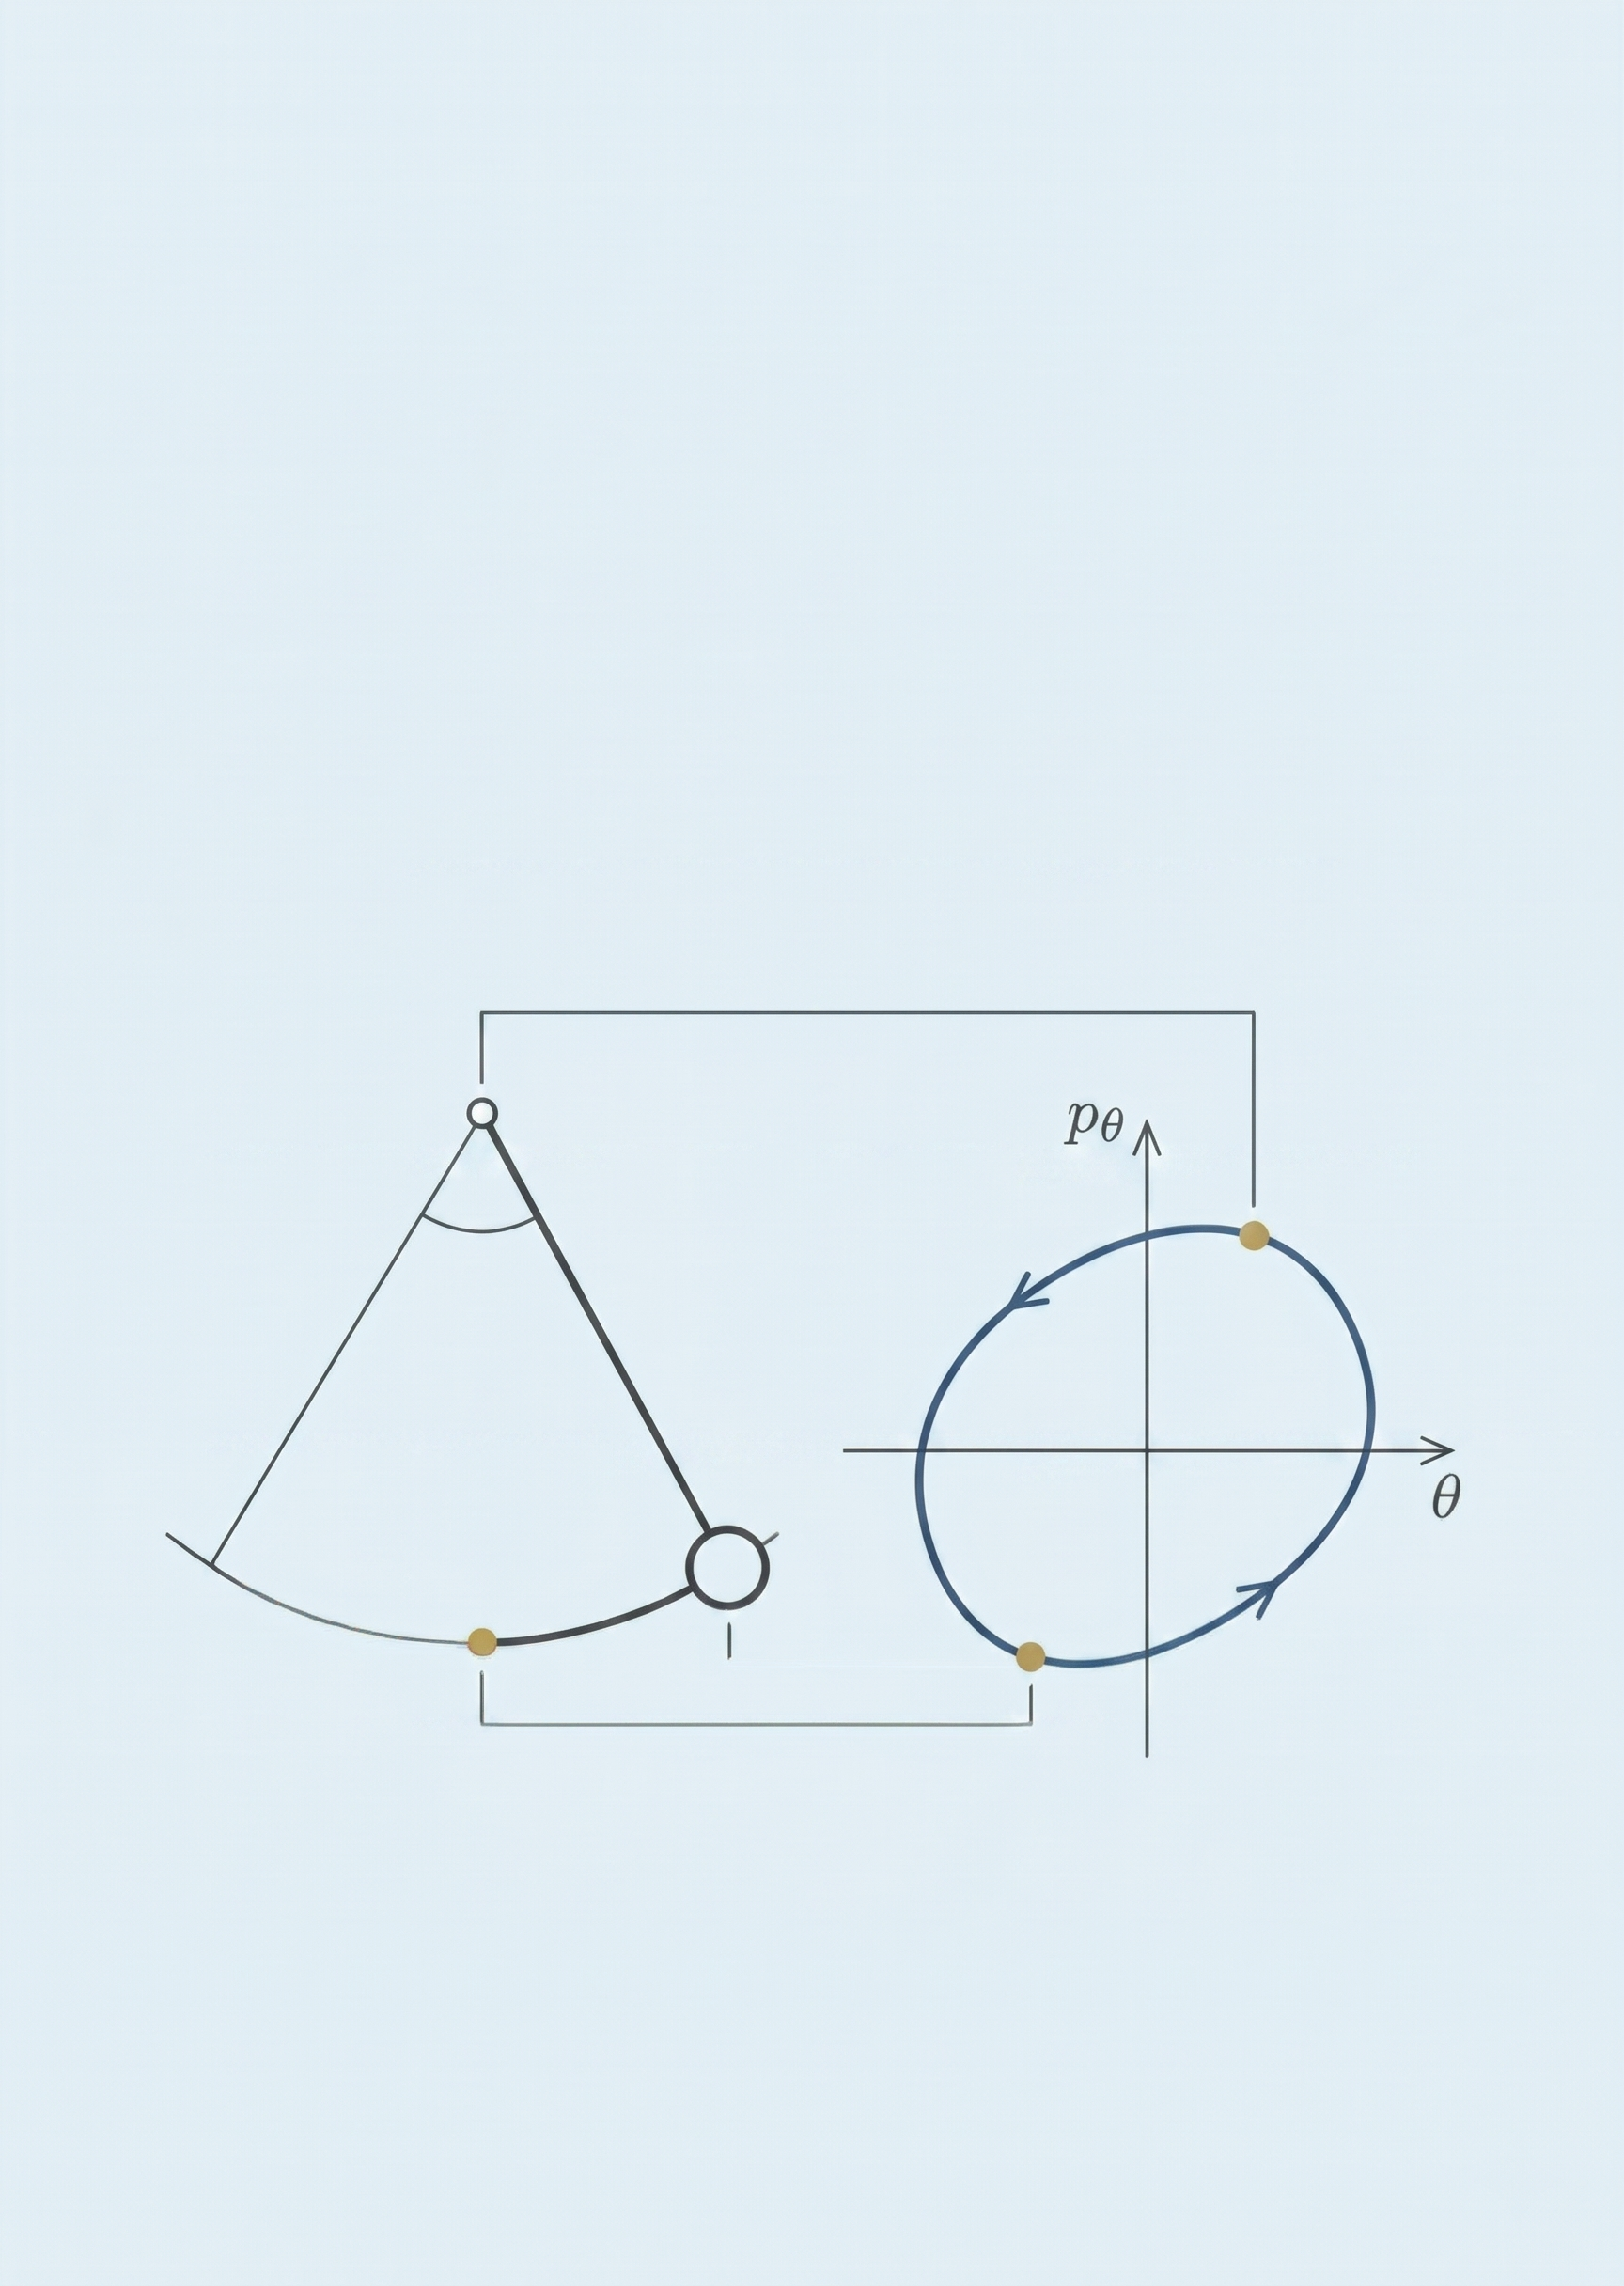
\includegraphics[height=\paperheight,keepaspectratio]{../../../generated_course_notes/core/classical_mechanics/2011_fall_theoretical_minimum/assets/cover-art.png}%
  };
  \node[
    anchor=north west,
    align=left,
    text width=0.78\paperwidth,
    fill=white,
    fill opacity=0.9,
    rounded corners=8pt,
    inner xsep=10pt,
    inner ysep=8pt
  ] at ([xshift=0.08\paperwidth,yshift=-0.06\paperheight]current page.north west) {%
    {\fontsize{30}{33}\selectfont\bfseries\color{black!88} Mécanique classique\\[0.85em]}
    {\large\color{black!72} Édition française / automne 2011, minimum théorique}
  };
  \node[
    anchor=south west,
    align=left,
    text width=0.68\paperwidth,
    fill=white,
    fill opacity=0.82,
    text opacity=1,
    rounded corners=6pt,
    inner sep=12pt
  ] at ([xshift=0.08\paperwidth,yshift=0.08\paperheight]current page.south west) {%
    {\normalsize\color{black!78} Cours originaux : Leonard Susskind\\[0.35em]}
    {\small\color{black!72} Édition d’accompagnement : \href{https://lazying.art}{LazyingArt LLC} / \href{https://github.com/lachlanchen/Video2Book}{Video2Book}}
  };
\end{tikzpicture}
\mbox{}
\end{titlepage}
\hypersetup{pageanchor=true}

\clearpage
\chapter{À propos de ces notes}
Ces notes complémentaires, éditées indépendamment, accompagnent les cours de Leonard Susskind. Elles ont été reconstituées à partir de transcriptions automatiques, de sous-titres et de certaines images du tableau, puis vérifiées à l’aide des sources disponibles. Elles ne constituent pas un manuscrit original du professeur Susskind et n’ont été ni relues ni approuvées par lui.

Cette édition a été préparée par \href{https://lazying.art}{LazyingArt LLC} à l’aide du flux de travail libre \href{https://github.com/lachlanchen/Video2Book}{Video2Book}. Les transcriptions automatiques restent disponibles séparément et peuvent comporter des erreurs de reconnaissance. Les précisions éditoriales et les reconstitutions substantielles sont signalées en notes de bas de page.
\clearpage
\tableofcontents
\mainmatter
\chapter{États, réversibilité et cinématique}

La mécanique classique ne se réduit pas à un ensemble d’équations décrivant des corps en chute, des planètes en orbite ou des particules chargées. Avant de choisir une équation particulière, nous pouvons poser une question plus générale : à quoi doit ressembler une loi du mouvement pour être considérée comme une loi classique ? Nous commencerons par des systèmes si simples que l’on peut dessiner au tableau toutes leurs évolutions possibles. Une fois les notions d’état, de déterminisme, de réversibilité et de conservation clarifiées dans ces systèmes, nous reviendrons aux particules se déplaçant dans l’espace ordinaire.

\section{Deux types de questions}

En mécanique, on peut poser deux types de questions. La première porte sur la loi particulière qui régit un système donné. Une planète qui se déplace dans le champ gravitationnel d’un corps massif obéit à une loi ; une particule chargée en mouvement dans un champ magnétique en obéit à une autre. Il s’agit de questions portant sur les lois détaillées de la nature.

L’autre question concerne le cadre commun à tous ces exemples. Existe-t-il des règles que toute loi admissible doit respecter ? Quelles caractéristiques relèvent de la mécanique classique elle-même, indépendamment de la force ou de l’objet étudié ? Les exemples particuliers nous aideront à répondre, mais c’est cette seconde question qui structure le sujet.

Le premier exemple le plus utile est celui d’une pièce abstraite posée sur une table abstraite. Nous ne retenons qu’une propriété de la pièce : elle peut tomber sur pile ou sur face. Son espace des configurations est donc
\begin{equation}
  \mathcal C=\{H,T\}.
\end{equation}
Le mot \emph{configuration} désigne l’une des façons dont le système peut se trouver. Une condition initiale consiste à en choisir une. Une pièce à une seule face serait encore plus simple, mais elle n’aurait qu’une configuration et rien ne pourrait jamais se produire. Deux états suffisent pour rendre une dynamique possible.

\section{La pièce : état, loi et évolution}

Faisons avancer le temps par pas entiers, comme si le monde était éclairé par un stroboscope :
\begin{equation}
  t=\ldots,-2,-1,0,1,2,\ldots .
\end{equation}
Une loi du mouvement est une règle de mise à jour. Elle associe à l’état à l’instant \(t\) un état à l’instant \(t+1\). La règle la plus simple ne change rien :
\begin{equation}
  H\longmapsto H,
  \qquad
  T\longmapsto T.
  \label{eq:coin-identity}
\end{equation}
En partant de \(H\), on obtient toute l’évolution \(H,H,H,\ldots\) ; en partant de \(T\), on obtient \(T,T,T,\ldots\). Cette règle est monotone, mais elle est parfaitement prédictive.

L’autre règle réversible échange les deux états :
\begin{equation}
  H\longmapsto T,
  \qquad
  T\longmapsto H.
  \label{eq:coin-flip}
\end{equation}
Les évolutions alternent alors :
\begin{equation}
  H,T,H,T,\ldots,
  \qquad
  T,H,T,H,\ldots .
\end{equation}
Une flèche va de l’état précédant la mise à jour à celui qui la suit. La base de la flèche indique donc l’état de départ du système, et sa pointe indique son état d’arrivée.

\begin{figure}[htbp]
  \centering
  \includegraphics[width=0.86\textwidth]{lecture_01_figure_02.png}
  \caption{Les deux configurations de la pièce et la loi de retournement orientée, dessinées au tableau pendant le cours. La règle de mise à jour épurée est donnée dans l’équation ~\eqref{eq:coin-flip}.}
  \lectureframe{00:06:50}
  \label{fig:coin-board}
\end{figure}

Nous pouvons coder les faces à l’aide d’une variable à deux valeurs,
\begin{equation}
  \sigma=
  \begin{cases}
    +1,&H,\\
    -1,&T.
  \end{cases}
\end{equation}
La lettre \(\sigma\) est traditionnellement utilisée en physique pour les grandeurs à deux valeurs, notamment dans les descriptions du spin, mais aucune connaissance du spin n’est nécessaire ici. Avec cette notation, les deux règles s’écrivent sous forme d’équations du mouvement :
\begin{align}
  \sigma(t+1)&=\sigma(t),
  &&\text{identity law},\label{eq:sigma-identity}\\
  \sigma(t+1)&=-\sigma(t),
  &&\text{flip law}.\label{eq:sigma-flip}
\end{align}
La variable n’ajoute pas de nouvelle physique. Elle fournit une étiquette compacte pour la configuration et transforme un graphe en équation.

\begin{figure}[htbp]
  \centering
  \includegraphics[width=0.86\textwidth]{lecture_01_figure_03.png}
  \caption{La loi de retournement écrite sous la forme \(\sigma(t+1)=-\sigma(t)\). Les valeurs encadrées \(\sigma=\pm1\) désignent pile et face.}
  \lectureframe{00:08:58}
  \label{fig:sigma-board}
\end{figure}

Pour l’une ou l’autre règle, l’état initial et la loi déterminent l’état à tout instant ultérieur. Cette affirmation suppose que le système est \emph{fermé}. Si quelqu’un intervient pour retourner la pièce, sa main exerce une influence extérieure qui ne figure pas dans notre description. Nous n’avons pas réfuté le déterminisme ; nous avons changé de système. Une loi classique est censée régir un système fermé, dont la description inclut toutes les influences pertinentes pour son évolution.

Il existe quatre fonctions mathématiques d’un ensemble à deux éléments vers lui-même. Les deux autres règles, non écrites plus haut, envoient les deux entrées sur \(H\) ou toutes deux sur \(T\). Elles sont déterministes vers le futur, mais effacent la distinction entre deux passés possibles. Lorsque nous imposerons la réversibilité ci-dessous, les équations ~\eqref{eq:coin-identity} et \eqref{eq:coin-flip} seront exactement les deux applications autorisées.

\section{Un dé : orbites et grandeurs conservées}

Remplaçons la pièce par un dé. Pour ce qui nous occupe, le seul fait important est qu’un dé possède six configurations,
\begin{equation}
  \mathcal C=\{1,2,3,4,5,6\}.
\end{equation}
Une condition initiale consiste à choisir un nombre. Nous pourrions, là encore, laisser chaque état fixe, mais les graphes orientés sont plus utiles pour étudier des règles moins triviales. Considérons
\begin{equation}
  1\longmapsto2\longmapsto3\longmapsto4
  \longmapsto5\longmapsto6\longmapsto1.
  \label{eq:six-cycle}
\end{equation}
Par exemple, en partant de \(4\), on obtient l’évolution suivante :

\[
  4,5,6,1,2,3,4,\ldots .
\]
Les six états forment un cycle unique.\footnote{Note sur la source : lors de la première lecture des flèches, une phrase prononcée indique que \(6\) revient à \(6\). La phrase qui suit immédiatement, le cycle dessiné et l’évolution énumérée donnent tous la mise à jour voulue : \(6\mapsto1\).}

\begin{figure}[htbp]
  \centering
  \includegraphics[width=0.86\textwidth]{lecture_01_figure_06.png}
  \caption{L’unique cycle à six états. À chaque pas stroboscopique, un état passe au suivant et revient à son point de départ après six mises à jour.}
  \lectureframe{00:12:40}
  \label{fig:six-cycle-board}
\end{figure}

Une règle peut sembler plus compliquée sans différer par sa structure. Par exemple,
\begin{equation}
  1\to2\to5\to3\to4\to6\to1
  \label{eq:relabeled-cycle}
\end{equation}
forme toujours un cycle unique à six états. Si l’on place les sommets sur la page dans l’ordre \(1,2,5,3,4,6\), on retrouve le même schéma que dans l’équation ~\eqref{eq:six-cycle}. Des étiquettes telles que \(1\) et \(5\) ne sont que des noms ; la structure du cycle n’en dépend pas.

Une loi véritablement différente répartit les six états en deux cycles, par exemple
\begin{equation}
  1\to2\to3\to1,
  \qquad
  4\to6\to5\to4.
  \label{eq:two-cycles}
\end{equation}
Il n’y a toujours qu’un seul dé et une seule loi, mais une trajectoire qui commence sur un cycle ne peut jamais atteindre l’autre. On peut attribuer aux cycles un nombre \(Q\) :
\begin{equation}
  Q=
  \begin{cases}
    0,&\text{on the cycle }\{1,2,3\},\\
    1,&\text{on the cycle }\{4,5,6\}.
  \end{cases}
\end{equation}
L’état change à chaque pas, tandis que \(Q\) reste constant.

\begin{definition}
Une grandeur conservée est une fonction de l’état dont la valeur reste inchangée sous l’action de la loi du mouvement.
\end{definition}

La même idée permet d’avoir un point fixe, un cycle de longueur deux et un cycle de longueur trois. L’étiquette conservée indique sur quelle orbite se trouve le système ; elle n’a pas besoin de préciser l’état au sein de cette orbite. La conservation est donc compatible avec le mouvement. Ce qui est préservé n’est pas nécessairement la configuration entière, mais une certaine distinction entre les configurations possibles.

\begin{figure}[htbp]
  \centering
  \includegraphics[width=0.86\textwidth]{lecture_01_figure_07.png}
  \caption{Plusieurs cycles disjoints au tableau : un point fixe, un cycle de longueur deux et un cycle de longueur trois. L’étiquette du cycle est conservée alors même que l’état parcourt celui-ci.}
  \lectureframe{00:18:40}
  \label{fig:conserved-cycles-board}
\end{figure}

Dans un système fini réversible, chaque trajectoire est un cycle. Un cycle unique ne peut pas porter d’étiquette conservée non constante de ce type élémentaire, car la trajectoire finit par visiter tous les états. La présence de plusieurs cycles permet une telle étiquette, puisque l’évolution ne fait jamais passer un état d’une composante à une autre.

\section{Que faut-il inclure dans un état ?}

Dans les exemples avec la pièce, la règle ne portait que sur un pas : la face suivante dépendait uniquement de la face présente. Une question du public permet de vérifier si cette restriction est essentielle.

\begin{classroomqa}
\audiencequestion{Peut-on construire une suite de piles et de faces dans laquelle le résultat suivant dépend de davantage que de la face immédiatement visible, par exemple d’un ou de plusieurs résultats antérieurs ?\lecturetimestamp{00:19:27--00:21:23}}

\lecturerresponse{Oui. Dans ce cas, \(H\) ou \(T\) à lui seul ne constitue pas l’état complet. S’il faut connaître la face précédente, élargissons l’espace des états à
\(
  \{HH,HT,TH,TT\}.
\)
Chaque paire ordonnée enregistre la face présente et celle qui la précède. On peut alors de nouveau écrire l’évolution comme une règle à un pas sur cet espace à quatre états. Si une histoire plus longue est nécessaire, il suffit d’inclure également ces informations.}
\end{classroomqa}

Cette réponse donne le sens opérationnel de la notion d’état.

\begin{definition}
À un instant donné, l’état d’un système comprend toutes les informations qui, avec la loi du mouvement, sont nécessaires pour prédire son évolution future.
\end{definition}

L’état n’est donc pas simplement une photographie. Il désigne l’ensemble complet de données qui rend l’évolution déterminée. Plus tard, lorsque nous décrirons une particule newtonienne, sa position ne suffira pas : la vitesse fera aussi partie des données initiales. La pièce dotée d’une mémoire illustre le même principe sous sa forme la plus simple.

\section{Espaces d’états infinis}

Un nombre infini d’états n’exige pas une infinité d’objets. Considérons une particule contrainte de se déplacer sur les sites entiers d’une droite infinie. Son état est un entier
\[
  n\in\mathbb Z.
\]
Une loi la fait avancer d’un site vers la droite à chaque pas :
\begin{equation}
  n(t+1)=n(t)+1.
  \label{eq:lattice-one}
\end{equation}
Cette orbite ne se referme jamais, mais, si on la suit dans le futur comme dans le passé, elle passe par tous les entiers. En ce sens élargi, elle joue le rôle d’un cycle sans fin.

Une autre loi la fait avancer de deux sites à la fois :
\begin{equation}
  n(t+1)=n(t)+2.
  \label{eq:lattice-two}
\end{equation}
Les sites pairs évoluent alors uniquement parmi les sites pairs, et les sites impairs uniquement parmi les sites impairs. La parité est conservée :
\begin{equation}
  \begin{aligned}
    Q_{\rm parity}(n)&=n\bmod 2,\\
    Q_{\rm parity}(n(t+1))&=Q_{\rm parity}(n(t)).
  \end{aligned}
\end{equation}
Le passage d’un espace de configurations fini à un espace infini permet des évolutions qui ne se répètent jamais, mais ne change pas le sens des notions d’état, d’orbite ou de conservation.

\section{Le déterminisme n’implique pas encore la réversibilité}

Dessinons maintenant une règle qui prédit le futur de façon univoque, mais qui échoue à satisfaire une deuxième exigence classique. Donnons à une pièce à trois côtés les états pile, face et tranche, et définissons
\begin{equation}
  H\to T,
  \qquad
  T\to E,
  \qquad
  E\to T.
  \label{eq:nonreversible-map}
\end{equation}
En partant de \(H\), on obtient l’évolution
\[
  H,T,E,T,E,\ldots;
\]
et, en partant de \(T\) ou de \(E\), l’alternance qui suit est tout aussi univoque. Chaque état possède exactement une flèche sortante : la règle est donc déterministe vers le futur.

La difficulté apparaît lorsque nous essayons de reconstruire le passé. Si l’état présent est \(T\), l’état précédent a pu être \(H\) ou \(E\). Deux évolutions ont fusionné. Si l’on inverse toutes les flèches, le défaut devient manifeste : à partir de \(T\), le graphe inversé offre deux mouvements possibles. La règle inversée n’est pas déterministe.

\begin{figure}[htbp]
  \centering
  \includegraphics[width=0.86\textwidth]{lecture_01_figure_08.png}
  \caption{La loi non réversible \(H,T,E\) et des évolutions représentatives. \(H\) et \(E\) mènent tous deux à \(T\) ; le présent ne détermine donc pas un passé unique.}
  \lectureframe{00:28:50}
  \label{fig:nonreversible-board}
\end{figure}

\begin{definition}
Une loi discrète est réversible si l’état présent détermine à la fois un état suivant unique et un état précédent unique. Dans un graphe d’états, chaque état doit avoir exactement une flèche entrante et une flèche sortante.
\end{definition}

Dans un espace d’états fini, une mise à jour réversible est une permutation des états. Elle ne crée ni ne détruit de distinctions entre les états ; elle ne fait que les réarranger. C’est pourquoi son graphe se décompose en cycles. L’application de l’équation ~\eqref{eq:nonreversible-map} est bien une fonction, mais elle n’est pas injective et n’a donc pas d’inverse.

\begin{classroomqa}
\audiencequestion{Une règle de ce type pourrait-elle être admise si les états représentaient des probabilités pour une particule ?\lecturetimestamp{00:29:46--00:31:17}}

\lecturerresponse{Ce serait un autre cadre théorique. La mécanique classique fondamentale, telle que nous la formulons ici, repose sur des lois déterministes plutôt que sur des règles de mise à jour probabilistes. On peut bien sûr inventer et étudier une telle règle, mais ce n’est pas une loi de mécanique classique en ce sens. La mécanique quantique n’est pas déterministe de la même manière et possède néanmoins un analogue de l’évolution réversible ; cela demandera une discussion ultérieure. La mécanique statistique classique fait aussi intervenir des probabilités, mais elle part de lois mécaniques sous-jacentes et représente notre connaissance incomplète des données initiales.}
\end{classroomqa}

Cette distinction est importante. Une distribution de probabilité utilisée parce que nous ignorons l’état classique exact ne constitue pas une loi du mouvement indéterministe. Elle décrit les informations dont nous disposons sur un système dont l’évolution microscopique est toujours supposée déterministe et réversible.

\section{Lois exactes et connaissance imparfaite}

La prédiction exige deux éléments :
\begin{enumerate}
  \item la loi du mouvement ;
  \item l’état initial.
\end{enumerate}
Une loi exacte ne permet pas d’obtenir une prévision exacte si la condition initiale n’est connue qu’approximativement. Pour la pièce, il est facile d’imaginer que l’on regarde la table et que l’on détermine parfaitement la face visible. Les variables mécaniques réelles sont continues. Les positions et les vitesses peuvent prendre des valeurs réelles quelconques, et aucune mesure ne fournit une infinité de décimales.

Supposons que l’état initial véritable appartienne à une petite région de l’espace des états possibles. Selon la dynamique, cette région peut rester petite pendant longtemps ; selon une autre, des états initiaux voisins peuvent diverger rapidement. Dans un système chaotique, de petites incertitudes initiales finissent par produire de grandes différences. L’atmosphère en est un exemple familier. Des mesures plus précises peuvent prolonger la période pendant laquelle la prévision est utile, mais, pour toute précision de mesure fixée, il existe un instant suffisamment éloigné où la prévision devient peu fiable.

Cette limite pratique n’introduit pas d’ambiguïté dans les équations. Si les conditions initiales étaient connues exactement, une loi classique réversible déterminerait aussi bien le futur que le passé. Avec une précision finie, la question quantitative est plutôt la suivante : avec quelle précision faut-il connaître l’état initial pour pouvoir prédire l’évolution sur une durée donnée ?

Le test graphique conduit à présent à une conclusion concise. Une loi représentée par exactement une flèche entrante et une flèche sortante en chaque état est déterministe et réversible. Les énoncés correspondants pour les particules seront moins élémentaires, mais ils exprimeront la même structure classique.

\section{Des états abstraits aux points de l’espace}

Passons maintenant des pièces et des dés aux particules ponctuelles. Une particule peut se déplacer dans une, trois, cinq dimensions, ou tout autre nombre de dimensions, mais l’espace ordinaire fournit un exemple immédiat. Pour décrire un point quantitativement, choisissons :
\begin{itemize}
  \item une origine ;
  \item trois axes mutuellement perpendiculaires ;
  \item une orientation de ces axes ;
  \item une unité de longueur.
\end{itemize}
Le choix de l’origine est conventionnel. On peut la placer à Palo Alto ou ailleurs, et les conclusions physiques ne devraient pas dépendre de ce choix. Les axes peuvent être notés \(x,y,z\) ou \(x_1,x_2,x_3\). Une fois les directions \(x\) et \(y\) fixées, l’axe \(z\) peut pointer dans l’un ou l’autre de deux sens perpendiculaires. Nous adoptons la convention directe : le pouce de la main droite pointant dans la direction \(x\) et l’index dans la direction \(y\), le majeur pointe dans la direction \(z\).

Des graduations identiques le long des axes exigent une unité, par exemple le mètre, le pied, le pouce ou l’année-lumière. Une fois ces conventions fixées, chaque point est repéré par trois nombres,
\begin{equation}
  (x,y,z).
\end{equation}
On peut atteindre le point depuis l’origine en se déplaçant le long des trois axes. Un système composé de plusieurs particules requiert un tel triplet pour chacune d’elles.

\begin{figure}[htbp]
  \centering
  \includegraphics[width=0.86\textwidth]{lecture_01_figure_09.png}
  \caption{Les axes cartésiens et les trois coordonnées d’un point. Le dessin fixe une convention de coordonnées ; le point lui-même ne dépend pas du choix de l’origine ou des axes.}
  \lectureframe{00:43:00}
  \label{fig:coordinates-board}
\end{figure}

\section{Vecteurs et composantes}

Un vecteur est un objet doté d’une norme et d’une direction. Le déplacement de l’origine à un point est un vecteur, mais les vecteurs servent aussi à décrire la vitesse, l’accélération, les champs électriques et bien d’autres grandeurs. Nous noterons un vecteur en caractères gras, par exemple \(\mathbf v\), et sa norme \(\lvert\mathbf v\rvert\). Cette norme est positive ou nulle, et ne s’annule que pour le vecteur nul.

Géométriquement, un vecteur est une flèche libre. La translater sans changer sa longueur ni sa direction ne change pas le vecteur. Dans une application donnée, un vecteur peut être attaché à un point, comme lorsqu’on spécifie le champ électrique en un lieu donné, mais cette attache est une information supplémentaire et ne fait pas partie du vecteur abstrait lui-même.

Dans un repère cartésien, un vecteur a pour composantes
\begin{equation}
  \mathbf v=(v_x,v_y,v_z).
\end{equation}
Les composantes sont des nombres signés ordinaires, obtenus par projection sur les axes. Elles codent à la fois la norme et la direction. Le théorème de Pythagore en trois dimensions donne
\begin{equation}
  \lvert\mathbf v\rvert^2
  =v_x^2+v_y^2+v_z^2,
  \qquad
  \lvert\mathbf v\rvert
  =\sqrt{v_x^2+v_y^2+v_z^2}.
  \label{eq:vector-magnitude}
\end{equation}
Les rapports entre les composantes déterminent la direction. Une composante négative signifie que le vecteur pointe en partie dans le sens négatif de l’axe correspondant.

\subsection{Multiplication par un scalaire et addition}

La multiplication par un nombre réel modifie la longueur d’un vecteur et, si ce nombre est négatif, en inverse la direction. Pour \(c>0\), \(c\mathbf A\) pointe dans la direction de \(\mathbf A\) et a pour norme \(c\lvert\mathbf A\rvert\). En particulier, \(-\mathbf A\) a la même longueur que \(\mathbf A\), mais pointe dans le sens opposé.

Il existe trois représentations équivalentes de l’addition vectorielle. Premièrement, plaçons l’origine de \(\mathbf B\) à la pointe de \(\mathbf A\) ; la flèche allant de l’origine de \(\mathbf A\) à la pointe de \(\mathbf B\) est \(\mathbf A+\mathbf B\).
Deuxièmement, plaçons les origines des deux vecteurs au même point et complétons un parallélogramme ; sa diagonale est leur somme. Cette construction rend visible la commutativité :
\begin{equation}
  \mathbf A+\mathbf B=\mathbf B+\mathbf A.
\end{equation}
Troisièmement, additionnons les composantes correspondantes :
\begin{equation}
  C_i=A_i+B_i,
  \qquad i=x,y,z,
  \label{eq:component-addition}
\end{equation}
où \(\mathbf C=\mathbf A+\mathbf B\). Ces règles définissent aussi des combinaisons linéaires quelconques, telles que \(a\mathbf A+b\mathbf B\).

\begin{figure}[htbp]
  \centering
  \includegraphics[width=0.86\textwidth]{lecture_01_figure_10.png}
  \caption{Les constructions du triangle et du parallélogramme pour l’addition vectorielle. Toutes deux donnent le même vecteur \(\mathbf A+\mathbf B\).}
  \lectureframe{00:53:00}
  \label{fig:vector-addition-board}
\end{figure}

Il n’existe pas d’opération générale permettant de diviser un vecteur par un autre. Il existe toutefois deux produits vectoriels usuels. Nous réserverons le produit vectoriel à un cours ultérieur. Ici, nous avons besoin du produit scalaire.

\subsection{Le produit scalaire}

Projetons \(\mathbf A\) sur l’axe défini par \(\mathbf B\). Si l’angle entre les vecteurs est \(\theta\), la composante algébrique de \(\mathbf A\) selon \(\mathbf B\) vaut \(\lvert\mathbf A\rvert\cos\theta\). La multiplication de cette projection par \(\lvert\mathbf B\rvert\) définit
\begin{equation}
  \mathbf A\cdot\mathbf B
  =\lvert\mathbf A\rvert\,\lvert\mathbf B\rvert\cos\theta.
  \label{eq:dot-geometric}
\end{equation}
Le résultat est un scalaire, et non un autre vecteur. L’équation ~\eqref{eq:dot-geometric} est symétrique par rapport à \(\mathbf A\) et \(\mathbf B\) ; ainsi, \(\mathbf A\cdot\mathbf B=\mathbf B\cdot\mathbf A\).

\begin{figure}[htbp]
  \centering
  \includegraphics[width=0.86\textwidth]{lecture_01_figure_11.png}
  \caption{Construction au tableau du produit scalaire par projection. La forme composée est \(\mathbf A\cdot\mathbf B=AB\cos\theta\).}
  \lectureframe{00:58:30}
  \label{fig:dot-product-board}
\end{figure}

Le signe fournit une information géométrique. Le produit scalaire est positif pour un angle aigu, négatif pour un angle obtus et nul pour des vecteurs perpendiculaires. Ainsi,
\begin{equation}
  \mathbf A\perp\mathbf B
  \quad\Longleftrightarrow\quad
  \mathbf A\cdot\mathbf B=0
\end{equation}
pour des vecteurs non nuls.

En composantes,
\begin{equation}
  \mathbf A\cdot\mathbf B
  =A_xB_x+A_yB_y+A_zB_z.
  \label{eq:dot-components}
\end{equation}
Cette formule permet d’effectuer directement les calculs. En particulier,
\begin{equation}
  \mathbf A\cdot\mathbf A
  =A_x^2+A_y^2+A_z^2
  =\lvert\mathbf A\rvert^2.
  \label{eq:self-dot}
\end{equation}
Étant données les composantes de deux vecteurs, les équations ~\eqref{eq:dot-geometric} et \eqref{eq:dot-components} déterminent l’angle qu’ils forment :
\begin{equation}
  \cos\theta
  =\frac{\mathbf A\cdot\mathbf B}
  {\lvert\mathbf A\rvert\,\lvert\mathbf B\rvert}.
\end{equation}

La loi des cosinus découle du même calcul. Soient \(\mathbf A\) et \(\mathbf B\) les vecteurs allant d’un même sommet aux deux autres sommets d’un triangle. Le troisième côté est
\(\mathbf C=\mathbf A-\mathbf B\), et non \(\mathbf A+\mathbf B\). Par conséquent,
\begin{align}
  C^2
  &=(\mathbf A-\mathbf B)\cdot(\mathbf A-\mathbf B)\notag\\
  &=A^2+B^2-2\mathbf A\cdot\mathbf B\notag\\
  &=A^2+B^2-2AB\cos\theta.
  \label{eq:law-of-cosines}
\end{align}

\begin{figure}[htbp]
  \centering
  \includegraphics[width=0.86\textwidth]{lecture_01_figure_04.png}
  \caption{Triangle utilisé pour la loi des cosinus. La correction apportée au tableau identifie le côté de fermeture comme étant \(\mathbf C=\mathbf A-\mathbf B\), ce qui conduit à l’équation ~\eqref{eq:law-of-cosines}.}
  \lectureframe{01:04:29}
  \label{fig:law-cosines-board}
\end{figure}

\section{Position, vitesse et accélération}

Choisissons une origine et notons \(\mathbf r\) le vecteur position allant de l’origine à une particule. Ses composantes sont les coordonnées cartésiennes :
\begin{equation}
  \mathbf r=(x,y,z),
  \qquad
  \lvert\mathbf r\rvert=\sqrt{x^2+y^2+z^2}.
\end{equation}
Changer d’origine modifie \(\mathbf r\) ; nous remettrons cette question à plus tard. Une fois l’origine fixée, le mouvement est décrit par une position dépendant du temps,
\begin{equation}
  \mathbf r(t)=\bigl(x(t),y(t),z(t)\bigr).
\end{equation}
La trajectoire est donc codée par trois fonctions du temps.

La vitesse est la dérivée temporelle de la position :
\begin{equation}
  \mathbf v(t)=\frac{d\mathbf r}{dt}
  =\dot{\mathbf r}(t),
  \qquad
  v_i=\frac{dx_i}{dt}=\dot x_i.
  \label{eq:velocity}
\end{equation}
Un point désigne toujours une dérivée par rapport au temps. La norme \(\lvert\mathbf v\rvert\) est la vitesse scalaire. En général, la position et la vitesse ont des directions indépendantes : en un lieu donné, une particule peut se déplacer dans toute direction permise par le problème.

L’accélération est le taux de variation de la vitesse, donc la dérivée seconde de la position par rapport au temps :
\begin{equation}
  \mathbf a(t)=\frac{d\mathbf v}{dt}
  =\dot{\mathbf v}(t)
  =\frac{d^2\mathbf r}{dt^2}
  =\ddot{\mathbf r}(t),
  \qquad
  a_i=\ddot x_i.
  \label{eq:acceleration}
\end{equation}
L’accélération est elle aussi un vecteur. Si une particule se déplaçant dans le sens positif de \(x\) accélère, \(a_x>0\). Si elle ralentit, \(a_x<0\). Ce qu’on appelle souvent une décélération est simplement une accélération opposée à la vitesse instantanée. Plus généralement, la vitesse peut changer de direction même si sa norme reste constante.

\begin{figure}[htbp]
  \centering
  \includegraphics[width=0.86\textwidth]{lecture_01_figure_05.png}
  \caption{Composantes de la vitesse écrites comme dérivées temporelles des composantes de la position. En notation vectorielle compacte, \(\mathbf v=d\mathbf r/dt\).}
  \lectureframe{01:14:24}
  \label{fig:velocity-board}
\end{figure}

\subsection{Accélération uniforme sur une droite}

Pour un mouvement à une dimension, écrivons
\begin{equation}
  x(t)=a+bt+ct^2.
  \label{eq:quadratic-motion}
\end{equation}
À l’instant \(t=0\), la particule se trouve en \(x=a\). Une puis deux dérivations donnent
\begin{align}
  v(t)=\dot x(t)&=b+2ct,\label{eq:line-velocity}\\
  a(t)=\ddot x(t)&=2c.\label{eq:line-acceleration}
\end{align}
Ainsi, \(b\) est la vitesse initiale et \(2c\) une accélération constante. Si \(c>0\), la vitesse augmente linéairement ; si \(c<0\), elle diminue linéairement. Cette loi quadratique pour la position décrit un mouvement à accélération constante, comme le mouvement idéalisé d’un corps en chute près de la surface terrestre.

\section{Mouvement circulaire uniforme}

Pour finir, considérons une particule se déplaçant dans le plan \(x\)-\(y\) sur le cercle unité. Elle part du point de l’axe \(x\) positif à l’instant \(t=0\), et sa coordonnée angulaire augmente uniformément :
\begin{equation}
  \theta(t)=\omega t.
\end{equation}
La constante \(\omega\) est la pulsation. Un tour correspond à une augmentation de l’angle de \(2\pi\) ; la période est donc
\begin{equation}
  T=\frac{2\pi}{\omega}.
  \label{eq:circular-period}
\end{equation}
On peut laisser l’angle augmenter au-delà de \(2\pi\) ; la position se répète, même si l’angle, enregistré de manière continue, ne revient pas à zéro.

Sur le cercle unité,
\begin{equation}
  \mathbf r(t)
  =\bigl(\cos\omega t,\,\sin\omega t\bigr).
  \label{eq:circular-position}
\end{equation}
La dérivation donne
\begin{equation}
  \mathbf v(t)
  =\omega\bigl(-\sin\omega t,\,\cos\omega t\bigr).
  \label{eq:circular-velocity}
\end{equation}
La vitesse est tangente au cercle. Nous pouvons démontrer qu’elle est perpendiculaire au rayon sans nous appuyer sur le dessin :
\begin{align}
  \mathbf r\cdot\mathbf v
  &=\cos\omega t\,(-\omega\sin\omega t)
    +\sin\omega t\,(\omega\cos\omega t)\notag\\
  &=0.
  \label{eq:r-dot-v}
\end{align}

\begin{figure}[htbp]
  \centering
  \includegraphics[width=0.86\textwidth]{lecture_01_figure_12.png}
  \caption{Composantes de la position et de la vitesse pour un mouvement sur le cercle unité. L’annulation dans \(\mathbf r\cdot\mathbf v\) vérifie que la vitesse est tangente au cercle.}
  \lectureframe{01:24:30}
  \label{fig:circular-velocity-board}
\end{figure}

En dérivant une nouvelle fois,
\begin{equation}
  \mathbf a(t)
  =-\omega^2
  \bigl(\cos\omega t,\,\sin\omega t\bigr)
  =-\omega^2\mathbf r(t).
  \label{eq:centripetal-acceleration}
\end{equation}
L’accélération est parallèle au rayon, mais pointe dans le sens opposé, vers le centre. C’est l’accélération centripète.\footnote{Note terminologique : le mot « ``centrifuge'' » apparaît à cet endroit du cours, mais l’équation et la description qui l’accompagne identifient l’accélération centripète usuelle, dirigée vers le centre.}

\begin{figure}[H]
  \centering
  \includegraphics[width=0.86\textwidth]{lecture_01_figure_13.png}
  \caption{Calcul des composantes de l’accélération circulaire. Chaque composante est égale à \(-\omega^2\) multiplié par la composante correspondante de la position ; ainsi, \(\mathbf a=-\omega^2\mathbf r\).}
  \lectureframe{01:26:30}
  \label{fig:circular-acceleration-board}
\end{figure}

Comme le rayon vaut un,
\begin{equation}
  \lvert\mathbf r\rvert=1,
  \qquad
  \lvert\mathbf v\rvert=\omega,
  \qquad
  \lvert\mathbf a\rvert=\omega^2.
\end{equation}
Augmenter \(\omega\) augmente linéairement la vitesse et quadratiquement l’accélération centripète nécessaire. Pour un cercle de rayon \(R\), le même calcul donnerait \(v=\omega R\) et \(\lvert\mathbf a\rvert=\omega^2R=v^2/R\) ; le cours utilise \(R=1\) afin de ne pas alourdir le premier calcul.

Nous disposons maintenant du langage élémentaire nécessaire à la mécanique des particules : états et données initiales, évolution réversible, coordonnées, vecteurs et dérivées définissant la vitesse et l’accélération. Il nous faut ensuite déterminer précisément quelles données initiales spécifient une particule et trouver les lois qui font évoluer ces données d’un instant au suivant.
\chapter{Forces, espace des phases et lois de conservation}

\lectureoverview{Une loi du mouvement doit faire plus que relier des grandeurs physiques familières. Elle doit spécifier l’état d’un système, faire évoluer cet état d’un instant au suivant et révéler quelles distinctions et quelles grandeurs subsistent au cours du mouvement. Nous aborderons la mécanique newtonienne en examinant d’abord une loi des forces plausible mais erronée, puis en élargissant l’état, de la position à l’espace des phases, et enfin en dérivant les lois de conservation de la quantité de mouvement et de l’énergie.}

\section{Une loi erronée, mais instructive}

Le mouvement quotidien est dominé par le frottement. Poussez un objet lourd sur un sol : il se déplace ; cessez de pousser et il s’arrête bientôt. En général, une poussée plus forte produit une vitesse plus grande, tandis qu’un objet plus lourd exige une poussée plus forte. Dans un tel monde, il est naturel de supposer que la force produit directement la vitesse. C’était l’intuition fondamentale qui sous-tendait la description aristotélicienne du mouvement.

Le patinage sur glace apporte l’expérience qui manque. Un patineur a besoin d’une force pour démarrer, s’arrêter ou changer de direction, mais pas pour continuer à glisser une fois en mouvement. Si Aristote avait travaillé sur une glace presque sans frottement plutôt que sur un sol ordinaire, le défaut de l’intuition force--vitesse aurait été beaucoup plus difficile à repérer.

Pour mettre en évidence ce qui cloche dans cette intuition, donnons-lui une formulation moderne précise. Écrivons l’équation délibérément incorrecte

\begin{equation}
  \mathbf F=m\mathbf v.
  \label{eq:aristotle-vector-law}
\end{equation}

Ce n’est pas la loi de Newton et il ne faut pas la mémoriser comme une loi physique. Elle est utile à titre diagnostique : une fois qu’une règle verbale est devenue une équation, nous pouvons demander si elle prédit le mouvement et si elle conserve suffisamment d’information pour reconstruire le passé. La brève discussion en classe du mot grec désignant la force renvoie à \emph{dynamis}, dont la racine se retrouve aussi dans des mots comme dynamo et dynamique ; mais la terminologie compte moins que la mise à l’épreuve de la loi elle-même.

\begin{figure}[htbp]\centering
  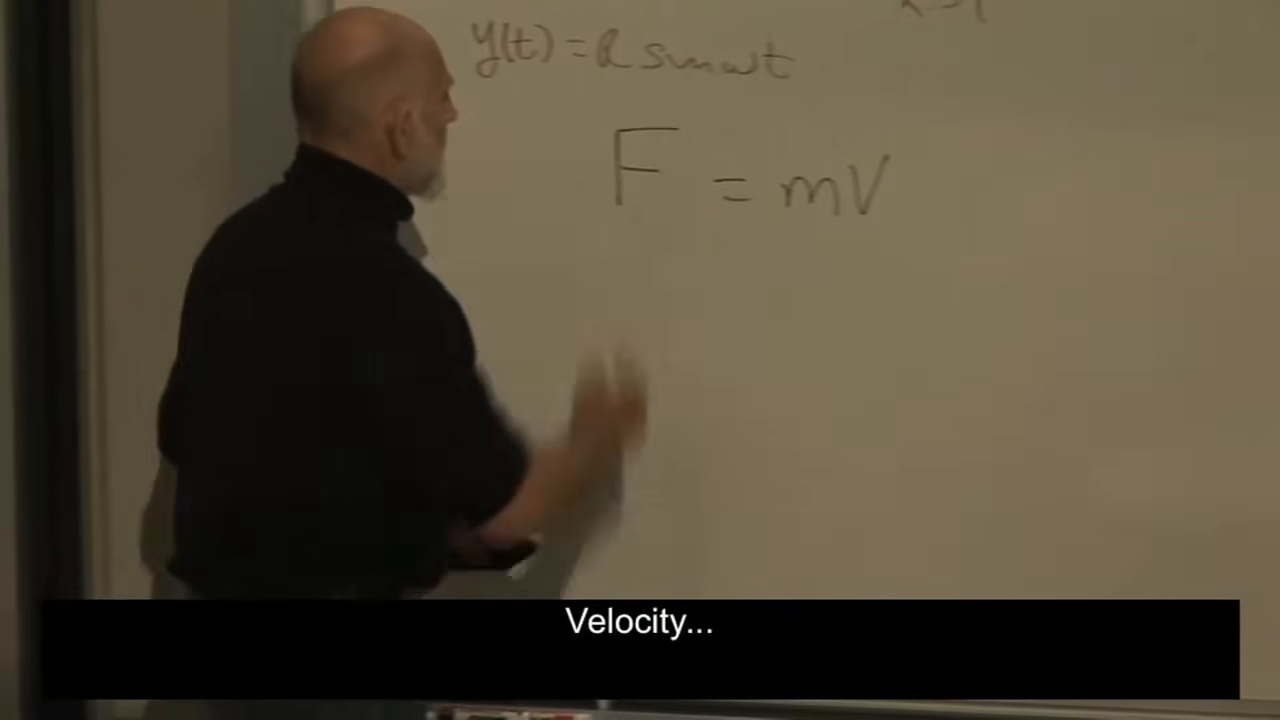
\includegraphics[width=0.82\textwidth]{lecture_02_figure_02.png}\caption{La loi force--vitesse, volontairement erronée, utilisée pour tester la prédictibilité et la réversibilité.}\lectureframe{00:04:51}\end{figure}

Restreignons le mouvement à une seule coordonnée spatiale. Puisque \(v=\dot x\), la loi s’écrit

\begin{equation}
  F(t)=m\dot x(t).
  \label{eq:aristotle-1d}
\end{equation}

Divisons maintenant le temps en courts intervalles de durée \(\delta\). Sur un intervalle,

\begin{equation}
  \dot x(t)\simeq
  \frac{x(t+\delta)-x(t)}{\delta}.
  \label{eq:first-difference}
\end{equation}

En substituant dans l’équation~\eqref{eq:aristotle-1d}, on obtient

\begin{equation}
  x(t+\delta)
  =x(t)+\frac{\delta}{m}F(t).
  \label{eq:aristotle-update}
\end{equation}

On a là la forme d’une véritable règle de mise à jour. Si l’on connaît la position actuelle et la force, on peut déterminer la position à l’instant stroboscopique suivant. Toutefois, lorsque la force s’annule, la règle d’Aristote donne \(\dot x=0\) : l’objet doit rester au repos. Le mouvement sans force d’entretien est exclu d’emblée.

\begin{figure}[htbp]\centering
  \includegraphics[width=0.84\textwidth]{lecture_02_figure_07.png}\caption{La mise à jour discrète d’Aristote avec une force de rappel. À chaque étape, le déplacement est multiplié par un facteur légèrement inférieur à un.}\lectureframe{00:10:15}\end{figure}

\subsection{Un ressort dans la mécanique d’Aristote}

Considérons une particule attachée à un ressort, dont la position d’équilibre est \(x=0\). Un déplacement produit la force de rappel

\begin{equation}
  F(x)=-kx,
  \qquad k>0.
  \label{eq:hooke-law}
\end{equation}

En introduisant cette force dans l’équation~\eqref{eq:aristotle-update}, on obtient

\begin{equation}
  x(t+\delta)
  =\left(1-\frac{k\delta}{m}\right)x(t).
  \label{eq:aristotle-spring-update}
\end{equation}

Pour \(\delta\) suffisamment petit, le facteur entre parenthèses est légèrement inférieur à un. Chaque mise à jour réduit donc le déplacement dans la même proportion :

\begin{equation}
  x_n=\left(1-\frac{k\delta}{m}\right)^n x_0.
  \label{eq:aristotle-geometric-decay}
\end{equation}

L’équation continue et sa solution sont

\begin{align}
  m\dot x&=-kx,
  \label{eq:aristotle-spring-continuous}\\
  x(t)&=x(0)e^{-kt/m}.
  \label{eq:aristotle-spring-solution}
\end{align}

Le ressort n’oscille pas. Quelle que soit la position initiale dont on la libère, la particule s’approche de l’origine de façon exponentielle, en ralentissant à mesure qu’elle s’en rapproche.

\begin{figure}[htbp]\centering
  \includegraphics[width=0.84\textwidth]{lecture_02_figure_08.png}\caption{La solution exponentielle de l’équation aristotélicienne du ressort. Le déplacement décroît au lieu d’osciller.}\lectureframe{00:12:02}\end{figure}

L’avenir est facile à prédire : tout déplacement initial tend vers la même configuration de repos. Pour le passé, c’est une autre affaire. Supposons que la particule soit observée très près de l’origine, avec une précision finie seulement. Elle aurait pu partir de n’importe laquelle de nombreuses positions distinctes, car leurs traces, devenues exponentiellement petites, finissent toutes par se trouver dans la même marge d’incertitude de mesure. Avec une précision mathématique parfaite, l’équation~\eqref{eq:aristotle-spring-solution} peut être résolue à rebours, mais les distinctions pratiques entre les histoires possibles s’effacent peu à peu. Du point de vue de la dynamique fondamentale réversible, cette loi est donc suspecte.

Cela ne signifie pas qu’Aristote était irrationnel. Le mouvement dominé par le frottement qu’il décrivait est effectivement dissipatif. Son erreur a été d’ériger ce comportement effectif en loi fondamentale. Le frottement est lui-même une force qui découle d’interactions microscopiques complexes. Lorsqu’une main pousse un objet à une vitesse à peu près constante, la force appliquée compense le frottement ; elle ne crée pas la vitesse en tant que telle.

\section{La loi de Newton et sa signification physique}

La correction apportée par Newton est que la force modifie le mouvement :

\begin{equation}
  \mathbf F=m\mathbf a=m\ddot{\mathbf x}.
  \label{eq:newton-second-law}
\end{equation}

Avant d’interpréter cette équation comme une équation d’évolution, il faut démêler deux apparentes circularités. La première concerne les référentiels. On entend souvent dire que les lois de Newton sont valables dans les référentiels inertiels et qu’un référentiel inertiel est un référentiel dans lequel ces lois sont valables. L’affirmation physique n’est pas cette définition circulaire. C’est l’énoncé empirique selon lequel il \emph{existe} des référentiels, décrits au moyen de règles et d’horloges appropriées, dans lesquels les lois de Newton prennent leur forme simple. Les référentiels qui accélèrent ou tournent par rapport à eux nécessitent des forces apparentes supplémentaires. Nous pourrons étudier plus tard la manière dont les équations se transforment dans ces autres référentiels.

La seconde circularité concerne la force et la masse. Si la force est définie comme le produit de la masse par l’accélération, et la masse comme le quotient de la force par l’accélération, l’équation semble vide de sens. Une expérience opérationnelle permet de distinguer les définitions de la loi. Comparons un objet à un kilogramme étalon en les équilibrant, puis attachons l’objet à un dynamomètre à ressort, dans un espace où n’agissent par ailleurs aucune force. Définissons une unité de force par un allongement fixe et faible du ressort. Deux ressorts identiques, allongés chacun de cette même quantité, fournissent deux unités de force et produisent une accélération double. Il est plus prudent d’ajouter un deuxième ressort que d’étirer un seul ressort deux fois plus, car un ressort réel finit par se comporter de manière non linéaire ou par casser. En gardant un seul ressort mais en lui attachant deux masses égales, on obtient la moitié de l’accélération ; avec trois masses égales, on en obtient le tiers.

\begin{figure}[htbp]\centering
  \includegraphics[width=0.84\textwidth]{lecture_02_figure_09.png}\caption{L’expérience de pensée du dynamomètre à ressort, utilisée pour définir des unités égales de force et vérifier que l’accélération est proportionnelle à la force.}\lectureframe{00:22:45}\end{figure}

Ces comparaisons donnent un contenu empirique à

\begin{equation}
  a\propto F,
  \qquad
  a\propto\frac{1}{m},
  \qquad
  F=ma.
  \label{eq:force-mass-scaling}
\end{equation}

Le mot \emph{particule} désignera tout petit objet dont la structure interne est sans importance, et pas seulement une particule élémentaire.

\subsection{Pourquoi la position seule ne suffit pas à définir un état}

Testons maintenant l’équation de Newton par la même méthode stroboscopique. La différence finie centrée de l’accélération est

\begin{equation}
  \ddot x(t)\simeq
  \frac{x(t+\delta)-2x(t)+x(t-\delta)}{\delta^2}.
  \label{eq:second-difference}
\end{equation}

L’équation de Newton implique donc

\begin{equation}
  x(t+\delta)
  =2x(t)-x(t-\delta)+\frac{\delta^2}{m}F(t).
  \label{eq:newton-position-update}
\end{equation}

La position suivante ne peut pas être obtenue à partir de \(x(t)\) seule. Il nous faut aussi la position précédente \(x(t-\delta)\), ou, de façon équivalente, la vitesse à l’instant présent. À première vue, l’équation de Newton semble donc moins prédictive que celle d’Aristote. La bonne conclusion est plutôt que la position seule ne décrivait pas complètement l’état. Connaître tout ce qui importe à un instant donné signifie disposer de suffisamment de données pour déterminer le mouvement ultérieur. Pour une particule newtonienne, ces données sont la position et la vitesse.

\section{Quantité de mouvement et espace des phases}

Introduisons la quantité de mouvement par

\begin{equation}
  \mathbf p=m\mathbf v=m\dot{\mathbf x}.
  \label{eq:momentum-definition}
\end{equation}

On considère que la masse d’un système newtonien donné est constante. Un objet peut perdre une pièce, comme un stylo peut perdre son capuchon, mais alors l’objet décrit a changé ; le système fermé choisi conserve, lui, une masse totale constante. Si \(m\) est constante, la deuxième loi de Newton devient

\begin{equation}
  \mathbf F=\dot{\mathbf p}.
  \label{eq:newton-momentum-form}
\end{equation}

\begin{figure}[htbp]\centering
  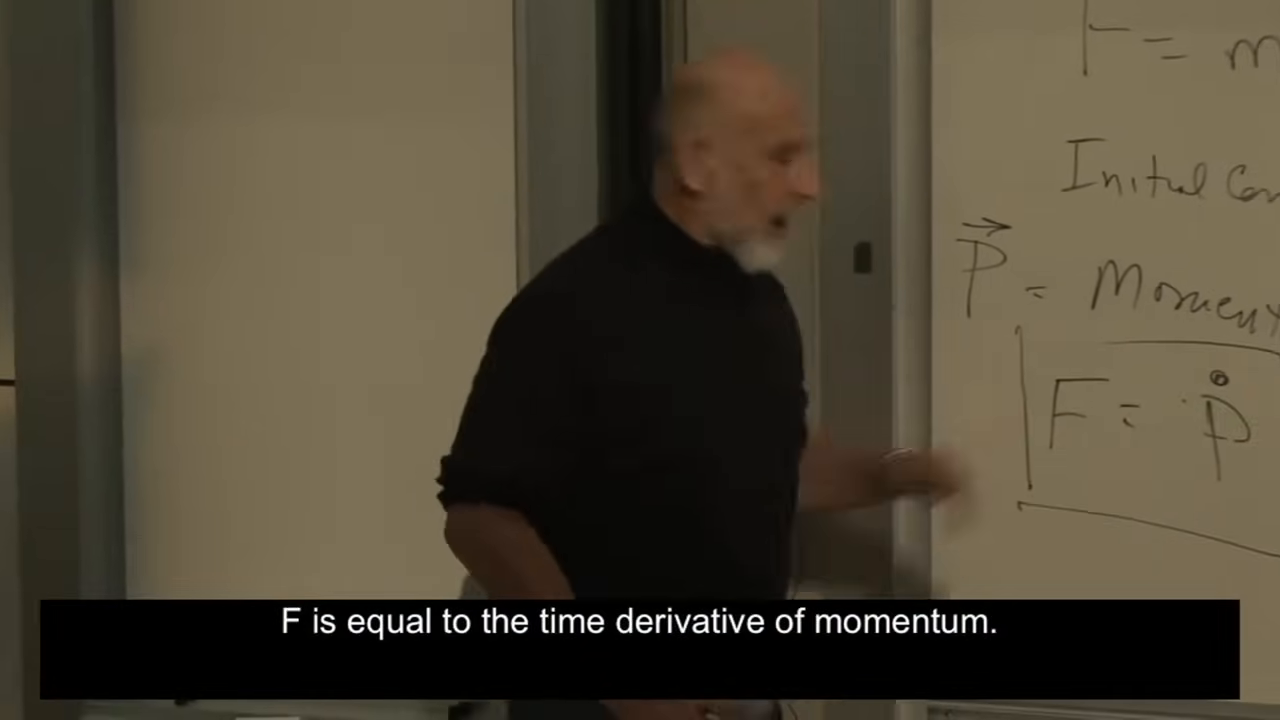
\includegraphics[width=0.82\textwidth]{lecture_02_figure_03.png}\caption{La loi de Newton écrite comme dérivée temporelle de la quantité de mouvement.}\lectureframe{00:32:35}\end{figure}

Pour une coordonnée, le mouvement newtonien peut maintenant s’écrire sous la forme de deux équations du premier ordre portant sur deux variables d’état indépendantes :

\begin{align}
  \dot p&=F(x,t),
  \label{eq:first-order-p}\\
  \dot x&=\frac{p}{m}.
  \label{eq:first-order-x}
\end{align}

L’une des équations indique comment la force modifie la quantité de mouvement ; l’autre, comment la quantité de mouvement modifie la position. Leur forme discrète du premier ordre est

\begin{align}
  p(t+\delta)&=p(t)+\delta F(x(t),t)+O(\delta^2),
  \label{eq:momentum-discrete}\\
  x(t+\delta)&=x(t)+\frac{\delta}{m}p(t)+O(\delta^2).
  \label{eq:position-discrete}
\end{align}

Étant données \(x(t)\) et \(p(t)\), ces équations déterminent la paire suivante, qui sert ensuite de données d’entrée pour l’étape suivante. La trajectoire se construit en répétant ces mises à jour.

\begin{figure}[htbp]\centering
  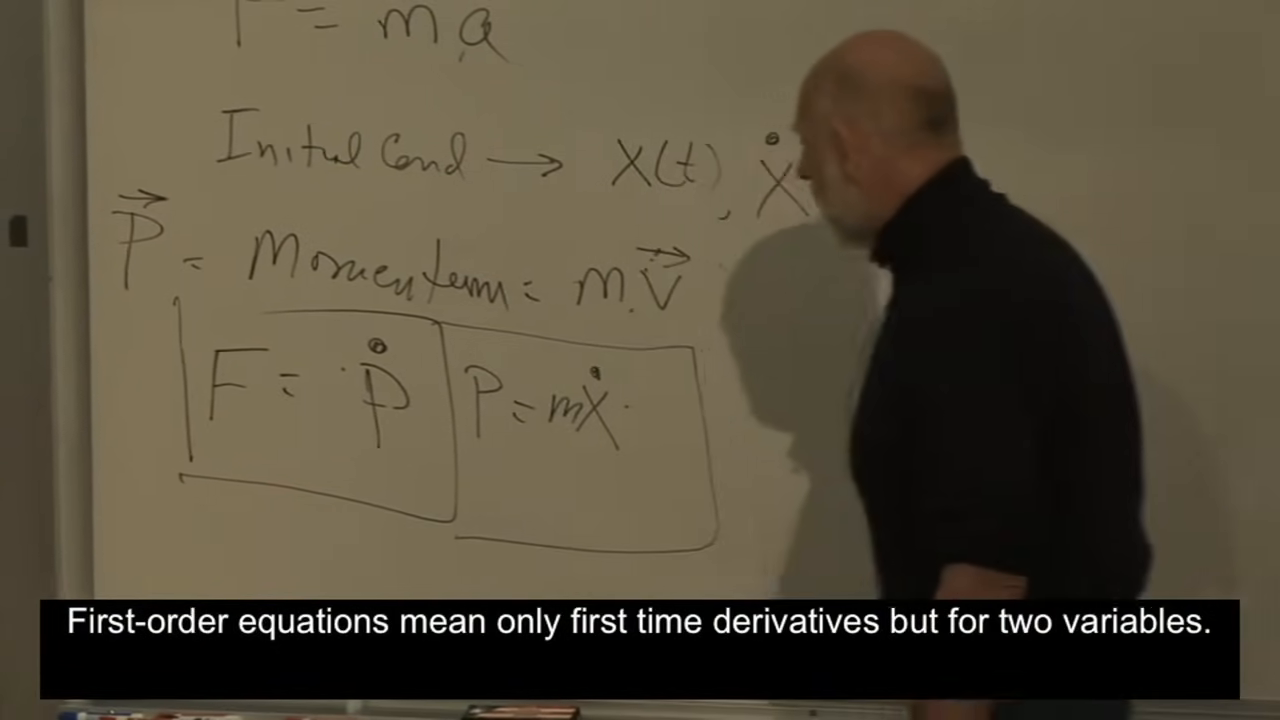
\includegraphics[width=0.84\textwidth]{lecture_02_figure_04.png}\caption{Les deux équations du premier ordre et les données initiales correspondantes. La position et la quantité de mouvement spécifient ensemble l’état.}\lectureframe{00:35:47}\end{figure}

L’ensemble de toutes les paires \((x,p)\) s’appelle l’\emph{espace des phases}. Pour une particule se déplaçant dans trois dimensions, il possède six coordonnées,

\begin{equation}
  (x,y,z,p_x,p_y,p_z).
  \label{eq:one-particle-phase-space}
\end{equation}

L’espace des phases est l’espace des conditions initiales complètes. L’espace des configurations ne décrit que les positions ; l’espace des phases contient précisément les données nécessaires à la loi du mouvement.

\begin{classroomqa}\audiencequestion{Si la force dépend de la position plutôt que du temps selon une fonction connue, la mise à jour devient-elle plus compliquée ?\lecturetimestamp{00:36:27--00:37:07}}\lecturerresponse{Les équations restent prédictives. Une fois que \(x\) et \(p\) sont connus, la valeur de \(F(x)\) est connue. L’équation~\eqref{eq:first-order-p} fait évoluer \(p\), l’équation~\eqref{eq:first-order-x} fait évoluer \(x\), et la paire mise à jour peut être réutilisée.}\end{classroomqa}

\section{Le ressort newtonien}

Revenons au ressort afin de comparer les deux lois dans des conditions physiques identiques. La loi de Newton donne

\begin{equation}
  m\ddot x=-kx.
  \label{eq:newton-spring}
\end{equation}

Posons provisoirement \(m=k=1\) afin d’éliminer les constantes. On obtient alors

\begin{equation}
  \ddot x=-x.
  \label{eq:normalized-oscillator}
\end{equation}

Contrairement à l’exponentielle, un sinus ou un cosinus retrouve son opposé après deux dérivations. La solution générale peut s’écrire

\begin{align}
  x(t)&=C\cos(t-t_0),
  \label{eq:oscillator-x}\\
  p(t)=\dot x(t)&=-C\sin(t-t_0).
  \label{eq:oscillator-p}
\end{align}

Les deux constantes portent les deux informations initiales. L’amplitude \(C\) donne le déplacement maximal, tandis que \(t_0\) fixe la phase, choisie ici de sorte que la vitesse s’annule en \(t=t_0\). La particule s’arrête uniquement de façon momentanée aux extrémités. Elle revient ensuite en passant par l’origine, où sa vitesse et sa quantité de mouvement sont maximales, puis poursuit ses oscillations.

En élevant au carré les équations~\eqref{eq:oscillator-x} et \eqref{eq:oscillator-p}, on obtient

\begin{equation}
  x^2+p^2=C^2.
  \label{eq:oscillator-phase-circle}
\end{equation}

Le point de l’espace des phases se déplace donc sur un cercle de rayon \(C\). Des amplitudes initiales différentes donnent des cercles différents ; modifier \(t_0\) choisit un autre point de départ sur le même cercle. Dans ces unités normalisées, tous les cercles sont parcourus avec la même période \(2\pi\), indépendamment de l’amplitude.

\begin{figure}[htbp]\centering
  \includegraphics[width=0.84\textwidth]{lecture_02_figure_10.png}\caption{Solution de l’oscillateur et orbite circulaire dans le plan de phase \((x,p)\).}\lectureframe{00:43:20}\end{figure}

\begin{figure}[htbp]\centering
  \begin{tikzpicture}[scale=1.05,>=Latex]
    \draw[->] (-2.6,0) -- (2.75,0) node[right] {$x$};
    \draw[->] (0,-2.4) -- (0,2.55) node[above] {$p$};
    \draw[blue!65!black,thick] (0,0) circle (1.85);
    \draw[->,blue!65!black,thick]
      (1.60,0.93) arc[start angle=30,end angle=72,radius=1.85];
    \fill[red!65!black] (1.60,0.93) circle (2pt);
    \draw[dashed] (0,0) -- (1.60,0.93)
      node[midway,below right] {$C$};
    \node[align=left] at (-1.55,1.85)
      {$x=C\cos(t-t_0)$\\$p=-C\sin(t-t_0)$};
  \end{tikzpicture}\caption{Une orbite dans l’espace des phases conserve la position et la quantité de mouvement. Son rayon caractérise le mouvement, tandis que l’angle évolue uniformément au cours du temps.}\label{fig:oscillator-phase-space}\end{figure}

La projection sur l’axe horizontal donne le mouvement de va-et-vient familier de \(x\) ; la projection sur l’axe vertical donne l’oscillation de \(p\). Contrairement au ressort aristotélicien, des cercles distincts ne se confondent jamais. La connaissance d’un point de l’espace des phases détermine à la fois le futur et le passé.

Pour des valeurs générales de \(m\) et \(k\), la pulsation angulaire est

\begin{equation}
  \omega=\sqrt{\frac{k}{m}},
  \qquad
  x(t)=C\cos\bigl(\omega(t-t_0)\bigr),
  \label{eq:general-oscillator-frequency}
\end{equation}

et l’orbite dans l’espace des phases devient une ellipse dans le plan \((x,p)\) non redimensionné. La représentation circulaire correspond à la normalisation commode \(m=k=1\) utilisée dans le cours.

\begin{classroomqa}\audiencequestion{Si, dans l’équation de l’oscillateur, on remplaçait la dérivée seconde par une dérivée première, la prédictibilité serait-elle perdue ?\lecturetimestamp{00:45:23--00:46:04}}\lecturerresponse{Non. Une équation du premier ordre peut quand même prédire le mouvement futur à partir de données initiales appropriées. La question plus profonde est de savoir si son flot préserve suffisamment les distinctions pour être réversible ; nous verrons le théorème général pertinent lorsque nous disposerons des outils nécessaires.}\end{classroomqa}

\section{Renversement du temps}

Le portrait de l’oscillateur rend la réversibilité concrète, mais les équations permettent aussi de la tester directement. Introduisons une coordonnée de temps renversé

\begin{equation}
  T=-t.
  \label{eq:reverse-time}
\end{equation}

On a alors

\begin{equation}
  \frac{d}{dt}=-\frac{d}{dT},
  \qquad
  \frac{d^2}{dt^2}=\frac{d^2}{dT^2}.
  \label{eq:time-derivative-parity}
\end{equation}

Une dérivée première change de signe sous le renversement du temps, contrairement à une dérivée seconde. Par conséquent, l’équation aristotélicienne autonome

\begin{equation}
  m\dot x=F(x)
  \label{eq:aristotle-time-reversal}
\end{equation}

ne conserve pas sa forme lorsqu’on passe le film à l’envers. Un ressort qui se rapproche de l’équilibre se mettrait à s’en éloigner spontanément. En revanche,

\begin{equation}
  m\ddot x=F(x)
  \label{eq:newton-time-reversal}
\end{equation}

reste inchangée. Lorsqu’on inverse un film newtonien, la vitesse s’inverse, mais l’accélération demeure inchangée ; le film inversé est donc une autre solution admissible.

\begin{figure}[htbp]\centering
  \includegraphics[width=0.84\textwidth]{lecture_02_figure_11.png}\caption{Comparaison au tableau sous la transformation \(t\mapsto -t\) : les dérivées premières changent de signe, contrairement aux dérivées secondes.}\lectureframe{00:50:45}\end{figure}

\begin{classroomqa}\audiencequestion{Pourquoi accepter la réversibilité comme principe général en physique ?\lecturetimestamp{00:46:16--00:48:26}}\lecturerresponse{On la met à l’épreuve ; elle n’est pas garantie par définition. Nous examinons les lois qui ont fait leurs preuves, repérons les caractéristiques communes aux expériences et érigeons celles-ci en principes. L’ordre logique plus profond est inverse : la théorie quantique des champs est plus fondamentale, et la mécanique newtonienne en émerge par des approximations telles que le mouvement lent et les objets massifs. Un cours doit progresser à partir de lois plus simples ; la réversibilité est donc introduite ici comme un principe dont la portée sera mise à l’épreuve par la suite.}\end{classroomqa}

\begin{classroomqa}\audiencequestion{Newton avait-il lui-même reconnu consciemment la réversibilité comme un problème ?\lecturetimestamp{00:48:28--00:49:02}}\lecturerresponse{La réponse historique est incertaine. Newton comprenait certainement l’inertie : une force est nécessaire pour modifier un état de mouvement, pas pour entretenir un mouvement uniforme. La question de savoir s’il a formulé explicitement cette idée en termes de réversibilité est une question historique distincte.}\end{classroomqa}

\section{Cycles et grandeurs conservées}

Les cercles de l’espace des phases suggèrent l’idée suivante. Une trajectoire reste sur un cercle donné et ne saute jamais sur un autre. On peut donc associer au cercle un nombre qui reste constant au cours du mouvement. Pour l’oscillateur normalisé, ce nombre est

\begin{equation}
  C^2=x^2+p^2.
  \label{eq:cycle-label}
\end{equation}

À un facteur deux près, il s’agit de l’énergie de l’oscillateur. Les cercles de plus grand rayon correspondent à une énergie plus élevée ; changer la phase initiale ne la modifie pas. Nous allons dériver ce résultat plutôt que de simplement le lire sur le schéma, mais considérons d’abord la quantité de mouvement.

La première loi de Newton affirme qu’un objet soumis à une force nette nulle se déplace à vitesse constante. Ce résultat est déjà contenu dans la deuxième loi :

\begin{equation}
  \mathbf F=0
  \quad\Longrightarrow\quad
  \dot{\mathbf p}=0
  \quad\Longrightarrow\quad
  \mathbf v=\text{constant}
  \label{eq:newton-first-from-second}
\end{equation}

lorsque la masse est constante. La troisième loi de Newton apporte une information véritablement nouvelle sur les interactions entre particules.

\subsection{Forces égales, opposées et centrales}

Notons \(\mathbf F_{ij}\) la force exercée sur la particule \(i\) par la particule \(j\). La relation d’égalité et d’opposition de la troisième loi s’écrit

\begin{equation}
  \mathbf F_{ij}=-\mathbf F_{ji}.
  \label{eq:newton-third-pair}
\end{equation}

Si les deux forces pointaient dans la même direction, une paire isolée pourrait accélérer spontanément. Elle constituerait une machine sans propulseur, produisant du mouvement par les seules forces internes. On n’observe pas un tel comportement.

\begin{figure}[htbp]\centering
  \includegraphics[width=0.84\textwidth]{lecture_02_figure_12.png}\caption{Énoncé indicé des forces d’interaction égales et opposées.}\lectureframe{00:59:25}\end{figure}

Pour les forces entre particules ponctuelles considérées ici, les forces de la paire agissent aussi le long de la droite qui joint les centres des particules. Des forces égales et opposées mais non colinéaires pourraient former un couple pur et mettre en rotation une paire rigide isolée. La condition de centralité empêche cette possibilité :

\begin{equation}
  \mathbf F_{ij}\parallel
  (\mathbf r_i-\mathbf r_j).
  \label{eq:central-force-condition}
\end{equation}

La condition d’égalité et d’opposition entraînera la conservation de la quantité de mouvement linéaire. La condition relative à la droite des centres est liée à la conservation du moment cinétique, qui sera étudiée plus tard.

\begin{figure}[htbp]\centering
  \includegraphics[width=0.84\textwidth]{lecture_02_figure_13.png}\caption{La condition de centralité dans la troisième loi de Newton : les forces d’interaction sont dirigées le long de la droite qui joint les particules.}\lectureframe{01:01:38}\end{figure}

\subsection{Quantité de mouvement totale}

Considérons un système fermé de \(N\) particules. Il n’y a aucune force extérieure ; les seules forces sont celles que les particules exercent les unes sur les autres. L’additivité des forces et la deuxième loi de Newton donnent, pour chaque particule,

\begin{equation}
  \dot{\mathbf p}_i
  =m_i\ddot{\mathbf r}_i
  =\sum_{\substack{j=1\\j\ne i}}^N \mathbf F_{ij}.
  \label{eq:many-particle-newton}
\end{equation}

Faisons la somme de cette équation sur \(i\) :

\begin{align}
  \frac{d}{dt}\sum_{i=1}^N\mathbf p_i
  &=\sum_{i=1}^N
    \sum_{\substack{j=1\\j\ne i}}^N\mathbf F_{ij}
  \notag\\
  &=\sum_{i<j}\bigl(\mathbf F_{ij}+\mathbf F_{ji}\bigr)
  =0.
  \label{eq:momentum-pair-cancellation}
\end{align}

Chaque interaction apparaît deux fois, une fois dans chaque sens, et les forces de la paire s’annulent. En définissant

\begin{equation}
  \mathbf P_{\mathrm{tot}}=\sum_{i=1}^N\mathbf p_i,
  \label{eq:total-momentum}
\end{equation}

on obtient la première loi de conservation :

\begin{equation}
  \frac{d\mathbf P_{\mathrm{tot}}}{dt}=0.
  \label{eq:momentum-conservation}
\end{equation}

\begin{figure}[htbp]\centering
  \includegraphics[width=0.84\textwidth]{lecture_02_figure_14.png}\caption{En sommant les équations des particules, les forces deux à deux s’annulent ; il ne reste que la dérivée de la quantité de mouvement totale, égale à zéro.}\lectureframe{01:04:38}\end{figure}

Historiquement, nous avons présenté la conservation de la quantité de mouvement comme une conséquence de la troisième loi de Newton. La physique moderne considère souvent cette conservation comme l’énoncé le plus fondamental : si un système isolé à deux particules conserve sa quantité de mouvement totale, les variations de leurs quantités de mouvement internes doivent être égales et opposées. Pour le développement présent, toutefois, la démarche newtonienne est la plus utile.

\section{Énergie en une dimension}

Considérons une particule se déplaçant sur une droite sous l’action d’une force qui dépend uniquement de sa position :

\begin{equation}
  F=F(x).
  \label{eq:position-force}
\end{equation}

Une telle force est dite indépendante du temps. Cela ne signifie pas que la valeur numérique de la force subie par la particule en mouvement soit constante. Sa valeur change lorsque \(x(t)\) change. Cela signifie que, chaque fois que la particule se trouve à la même position \(x\), elle subit la même force, quelle que soit l’heure indiquée par l’horloge.

En une dimension, toute fonction de force suffisamment régulière peut être intégrée. Nous définissons donc une énergie potentielle \(V(x)\) par

\begin{equation}
  F(x)=-\frac{dV}{dx},
  \label{eq:potential-definition-1d}
\end{equation}

ou, de manière équivalente,

\begin{equation}
  V(x)=-\int^x F(u)\,du+V_0.
  \label{eq:potential-integral}
\end{equation}

La constante additive \(V_0\) n’a aucun effet sur la force. Représentons \(V(x)\) comme la hauteur d’un paysage au-dessus de l’axe \(x\). La particule est poussée vers les hauteurs plus faibles, et la force est d’autant plus grande que la pente est raide. Au sommet ou au creux d’une colline lisse, la pente s’annule, et la force aussi.

\begin{figure}[htbp]\centering
  \includegraphics[width=0.84\textwidth]{lecture_02_figure_15.png}\caption{L’énergie potentielle comme paysage unidimensionnel. La force est dirigée vers le bas de la pente et son intensité est déterminée par la pente.}\lectureframe{01:12:57}\end{figure}

Définissons les énergies cinétique, potentielle et totale par

\begin{equation}
  T=\frac12m\dot x^2,
  \qquad
  E=T+V(x)
  =\frac12m\dot x^2+V(x).
  \label{eq:energy-1d}
\end{equation}

À ce stade, énergie est simplement le nom donné à cette quantité candidate à la conservation. Le paysage suggère son interprétation physique : en descendant la pente, \(V\) diminue tandis que la vitesse augmente, et donc \(T\) aussi ; en remontant la pente, c’est l’inverse. L’équation de Newton démontre que cet échange est exact.

Dérivons l’équation~\eqref{eq:energy-1d}. Puisque \(m\) est constante et que \(V\) ne dépend du temps qu’à travers \(x(t)\),

\begin{align}
  \frac{dE}{dt}
  &=m\dot x\ddot x+\frac{dV}{dx}\dot x
  \notag\\
  &=\dot x\left(m\ddot x+\frac{dV}{dx}\right).
  \label{eq:energy-derivative-1d}
\end{align}

La loi de Newton et la définition de \(V\) donnent

\begin{equation}
  m\ddot x=F=-\frac{dV}{dx}.
  \label{eq:newton-potential-1d}
\end{equation}

Le terme entre crochets dans l’équation~\eqref{eq:energy-derivative-1d} s’annule donc :

\begin{equation}
  \frac{dE}{dt}=0.
  \label{eq:energy-conservation-1d}
\end{equation}

\begin{figure}[htbp]\centering
  \includegraphics[width=0.84\textwidth]{lecture_02_figure_16.png}\caption{La dérivée de l’énergie unidimensionnelle, factorisée en un produit de la vitesse par l’équation de Newton.}\lectureframe{01:19:18}\end{figure}

En une dimension, aucune hypothèse dynamique supplémentaire n’était nécessaire au-delà d’une force régulière dépendant de la position, car toute force de ce type possède une primitive.

\section{Plusieurs dimensions et forces conservatives}

Pour une particule de coordonnées \(x_i\), l’équation de Newton se décompose en

\begin{equation}
  F_i(\mathbf x)=m\ddot x_i.
  \label{eq:newton-components}
\end{equation}

La composante \(F_i\) de la force peut dépendre de toutes les coordonnées, et pas seulement de \(x_i\). Nous aimerions trouver une fonction scalaire unique \(V(\mathbf x)\) telle que

\begin{equation}
  F_i(\mathbf x)
  =-\frac{\partial V(\mathbf x)}{\partial x_i},
  \qquad
  \mathbf F=-\boldsymbol\nabla V.
  \label{eq:gradient-force}
\end{equation}

Contrairement à la construction unidimensionnelle, cela n’est pas automatique. Trois fonctions arbitraires \(F_1,F_2,F_3\) contiennent en général davantage d’informations indépendantes que les dérivées d’une seule fonction scalaire. De manière équivalente, un potentiel n’existe que si le champ de forces satisfait des conditions de compatibilité, telles que l’égalité des dérivées partielles mixtes appropriées ; dans une région simplement connexe, cela s’exprime par \(\boldsymbol\nabla\times\mathbf F=0\). Nous posons donc l’équation~\eqref{eq:gradient-force} comme un postulat physique pour la classe de forces considérée, et non comme une identité mathématique.

\begin{figure}[htbp]\centering
  \includegraphics[width=0.84\textwidth]{lecture_02_figure_17.png}\caption{La loi des forces en plusieurs dimensions et un schéma des courbes de niveau du potentiel. La force pointe à travers les courbes de niveau, vers les valeurs décroissantes de \(V\).}\lectureframe{01:24:15}\end{figure}

Sur une carte de contours, \(V\) est constant le long de chaque courbe de niveau. Le gradient est perpendiculaire à ces courbes et pointe dans la direction de la plus forte augmentation ; la force \(-\boldsymbol\nabla V\) pointe dans la direction de la plus forte diminution.

\begin{figure}[htbp]\centering
  \begin{tikzpicture}[scale=1.0,>=Latex]
    \draw[->] (-3.0,0) -- (3.1,0) node[right] {$x_1$};
    \draw[->] (0,-2.4) -- (0,2.55) node[above] {$x_2$};
    \draw[orange!65!black,thick]
      plot[smooth cycle] coordinates
      {(-0.55,-0.35) (0.15,-0.55) (0.72,-0.10) (0.50,0.53) (-0.25,0.65)};
    \draw[orange!65!black,thick]
      plot[smooth cycle] coordinates
      {(-1.15,-0.75) (0.20,-1.10) (1.35,-0.25) (1.10,0.95) (-0.45,1.25)};
    \draw[orange!65!black,thick]
      plot[smooth cycle] coordinates
      {(-1.85,-1.20) (0.15,-1.70) (2.15,-0.40) (1.70,1.50) (-0.80,1.85)};
    \draw[->,blue!65!black,very thick] (1.62,0.73) -- (0.82,0.20)
      node[midway,above left] {$\mathbf F$};
    \draw[dashed,->,red!65!black,thick] (0.82,0.20) -- (1.62,0.73)
      node[midway,below right] {$\boldsymbol\nabla V$};
    \node[orange!65!black] at (-1.62,1.45) {$V=V_3$};
    \node[orange!65!black] at (-0.92,0.92) {$V=V_2$};
    \node[orange!65!black] at (-0.35,0.30) {$V=V_1$};
  \end{tikzpicture}\caption{Courbes de niveau d’un potentiel scalaire. Le gradient est normal aux courbes de niveau, et une force conservative pointe dans la direction opposée.}\label{fig:potential-contours}\end{figure}

Lorsque l’équation~\eqref{eq:gradient-force} est vérifiée, définissons

\begin{equation}
  E=\frac12m\sum_i\dot x_i^2+V(x_1,\ldots,x_n).
  \label{eq:energy-many-coordinates}
\end{equation}

Le terme cinétique est égal à la moitié du produit de la masse par le carré de la norme du vecteur vitesse. En dérivant et en appliquant la règle de dérivation en chaîne pour plusieurs variables, on obtient

\begin{align}
  \frac{dE}{dt}
  &=m\sum_i\dot x_i\ddot x_i
    +\sum_i\frac{\partial V}{\partial x_i}\dot x_i
  \notag\\
  &=\sum_i\dot x_i
    \left(m\ddot x_i+\frac{\partial V}{\partial x_i}\right)
  =0.
  \label{eq:energy-derivative-multidimensional}
\end{align}

La démonstration est exactement celle du cas unidimensionnel, avec un indice en plus, mais son hypothèse est plus forte : toutes les composantes de la force doivent dériver d’un même potentiel.

\begin{figure}[htbp]\centering
  \includegraphics[width=0.84\textwidth]{lecture_02_figure_18.png}\caption{Dérivée indicée de l’énergie. Chaque terme entre crochets s’annule grâce à la composante correspondante de l’équation de Newton.}\lectureframe{01:28:30}\end{figure}

Pour \(N\) particules en trois dimensions, rassemblons toutes les coordonnées dans une seule liste

\begin{equation}
  \begin{aligned}
    q_a={}&(x_1,y_1,z_1,x_2,y_2,z_2,\ldots,\\[-0.2em]
           &\phantom{(}x_N,y_N,z_N),\\
    &a=1,\ldots,3N.
  \end{aligned}
  \label{eq:flattened-coordinates}
\end{equation}

Il y a \(3N\) coordonnées, mais seulement \(N\) masses ; une même masse intervient dans les trois coordonnées associées à une particule donnée. Si

\begin{equation}
  F_a=-\frac{\partial V(q_1,\ldots,q_{3N})}{\partial q_a},
  \label{eq:many-particle-conservative-force}
\end{equation}

alors

\begin{equation}
  E=\sum_{A=1}^{N}\frac12m_A\lvert\dot{\mathbf r}_A\rvert^2
    +V(\mathbf r_1,\ldots,\mathbf r_N)
  \label{eq:many-particle-energy}
\end{equation}

est conservée par le même calcul. Les forces qui dérivent d’un potentiel sont dites \emph{conservatives} précisément parce qu’elles permettent cette loi de conservation ; l’adjectif n’a aucun sens politique.

\section{L’oscillateur comme courbe de niveau d’énergie}\enlargethispage{3\baselineskip}

Pour la force de rappel du ressort \(F=-kx\), l’équation~\eqref{eq:potential-definition-1d} donne

\begin{equation}
  V(x)=\frac12kx^2+V_0.
  \label{eq:spring-potential}
\end{equation}

En choisissant \(V_0=0\), l’énergie de l’oscillateur est

\begin{equation}
  E=\frac12m\dot x^2+\frac12kx^2
   =\frac{p^2}{2m}+\frac12kx^2.
  \label{eq:oscillator-energy}
\end{equation}

Pour \(m=k=1\),

\begin{equation}
  2E=p^2+x^2=C^2.
  \label{eq:oscillator-energy-circle}
\end{equation}

Les cercles de l’espace des phases obtenus précédemment sont donc des courbes de niveau d’énergie constante. Pour un potentiel unidimensionnel plus général, ces courbes ne sont pas nécessairement circulaires, mais le mouvement reste situé sur des courbes

\begin{equation}
  \frac{p^2}{2m}+V(x)=E
  \label{eq:general-energy-contour}
\end{equation}

dans le plan \((x,p)\). Nous retrouvons ainsi l’idée de la première leçon : lorsque les trajectoires restent sur des cycles ou des orbites distincts, un nombre peut caractériser ces orbites et rester inchangé tout au long du mouvement.

Nous disposons maintenant de l’espace des états, des équations de mise à jour newtoniennes et des deux premières lois de conservation. La prochaine formulation de la mécanique partira du principe de moindre action et conduira aux lagrangiens, aux hamiltoniens, au moment cinétique et à la structure plus générale qui sous-tend ces exemples.

\begin{classroomqa}\audiencequestion{Dans quelle mesure le polycopié distribué correspond-il au travail effectué au tableau, et où sont les figures ?\lecturetimestamp{01:37:56--01:38:54}}\lecturerresponse{Le polycopié devrait suivre de près le cours ; si certains éléments présentés au tableau n’y figurent pas, il se peut que le mauvais fichier ait été envoyé. Les figures n’étaient pas encore prêtes ; comme il le plaisante, elles arriveraient quand la formation continue paierait le prochain chèque.}\end{classroomqa}
\chapter{Action stationnaire et équation d’Euler--Lagrange}

\lectureoverview{Le nom traditionnel de \emph{principe de moindre action} en masque l’idée essentielle : la trajectoire physique rend l’action stationnaire, sans nécessairement la minimiser. Nous établirons cette affirmation à partir de l’équilibre ordinaire, l’étendrons des points aux fonctions entières, déduirons l’équation d’Euler--Lagrange en discrétisant une trajectoire, puis retrouverons les équations de Newton. Enfin, les coordonnées tournantes et polaires montreront que la formulation lagrangienne ne se réduit pas à un changement de notation.}

\section{Stationnaire, pas nécessairement minimale}

Dans le nom traditionnel, c’est le mot \emph{moindre} qui prête à confusion. Une trajectoire classique ne rend pas toujours l’action minimale. Elle peut plutôt lui donner un maximum ou un point selle dans l’espace des trajectoires possibles. Le principe correct est que l’action est \emph{stationnaire} : sa variation au premier ordre s’annule.

Commençons par la question plus simple de l’équilibre. Une particule qui reste au repos n’a pas d’accélération ; la résultante des forces doit donc être nulle. Pour une force dérivant d’un potentiel unidimensionnel,
\begin{equation}
  F(x)=-\frac{dV}{dx},
  \label{eq:force-from-v}
\end{equation}
la condition d’équilibre s’écrit
\begin{equation}
  \frac{dV}{dx}=0.
  \label{eq:stationary-v-one}
\end{equation}

\begin{figure}[htbp]
  \centering
  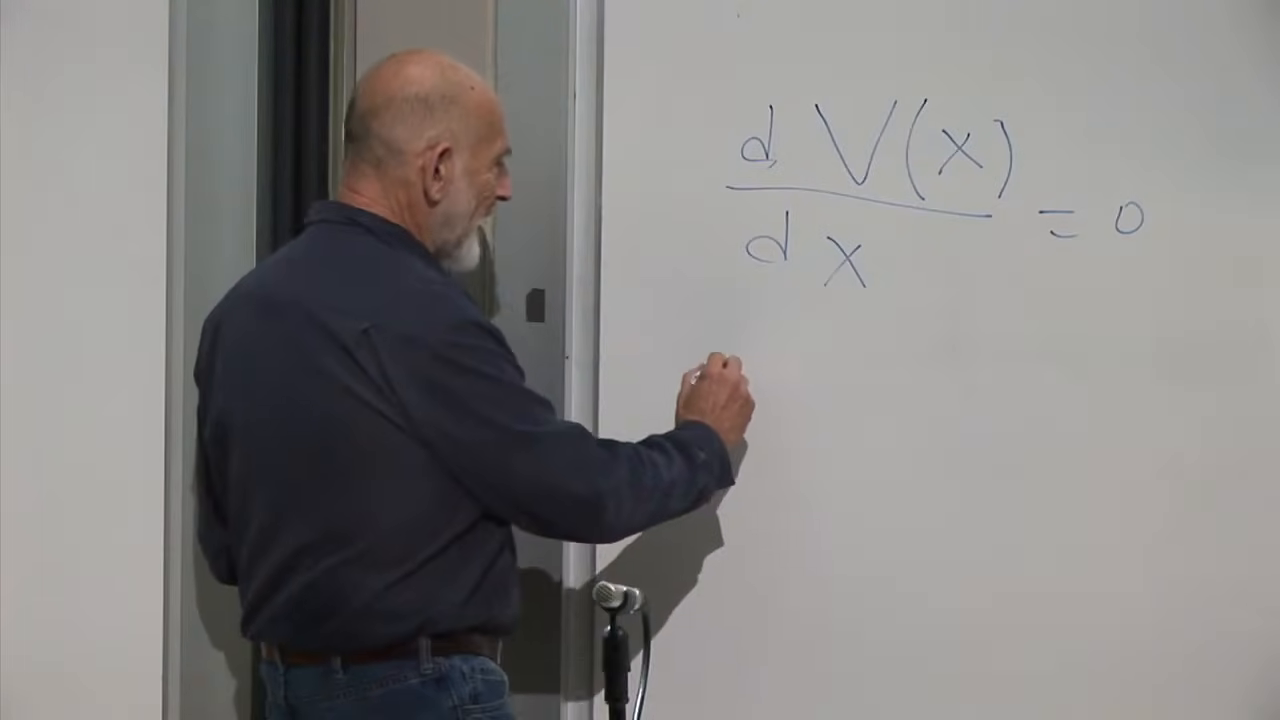
\includegraphics[width=0.74\textwidth]{lecture_03_figure_02.png}
  \caption{Condition d’équilibre en une dimension : la force s’annule là où le potentiel est stationnaire.}
  \lectureframe{00:02:51}
\end{figure}

Déplaçons maintenant la particule d’une petite quantité \(\delta x\). Au premier ordre,
\begin{equation}
  \delta V
  =V(x+\delta x)-V(x)
  =\frac{dV}{dx}\,\delta x+O(\delta x^2).
  \label{eq:first-variation-one}
\end{equation}
À l’équilibre, le terme linéaire est nul quel que soit le signe de \(\delta x\) :
\begin{equation}
  \delta V=0
  \qquad\hbox{to first order.}
  \label{eq:delta-v-zero-one}
\end{equation}
Cela ne signifie pas que \(V\) reste exactement inchangé après un déplacement fini. Cela signifie que sa variation dominante est quadratique ou d’ordre supérieur. Un minimum comme un maximum vérifie cette condition.

\begin{figure}[htbp]
  \centering
  \begin{tikzpicture}[scale=0.95,>=Latex]
    \draw[->] (-0.2,0) -- (3.35,0) node[right] {$x$};
    \draw[->] (0,-0.2) -- (0,2.25) node[above] {$V$};
    \draw[blue!65!black,thick,smooth]
      plot coordinates {(0.2,1.85) (0.75,0.85) (1.55,0.35)
                        (2.35,0.85) (3.0,1.85)};
    \fill[red!65!black] (1.55,0.35) circle (2pt);
    \node at (1.55,-0.34) {minimum};
    \begin{scope}[xshift=4.25cm]
      \draw[->] (-0.2,0) -- (3.35,0) node[right] {$x$};
      \draw[->] (0,-0.2) -- (0,2.25) node[above] {$V$};
      \draw[blue!65!black,thick,smooth]
        plot coordinates {(0.2,0.35) (0.75,1.25) (1.55,1.85)
                          (2.35,1.25) (3.0,0.35)};
      \fill[red!65!black] (1.55,1.85) circle (2pt);
      \node at (1.55,-0.34) {maximum};
    \end{scope}
  \end{tikzpicture}
  \caption{La stationnarité fixe la dérivée première, mais ne dit pas si le point est un minimum ou un maximum.}
  \label{fig:min-max-stationary}
\end{figure}

Pour plusieurs coordonnées \(q_i\), la première variation vaut
\begin{equation}
  \delta V
  =\sum_i\frac{\partial V}{\partial q_i}\,\delta q_i.
  \label{eq:first-variation-many}
\end{equation}
Si elle doit s’annuler pour tout déplacement infinitésimal indépendant
\(\delta q_i\), alors chacun des coefficients s’annule :
\begin{equation}
  \frac{\partial V}{\partial q_i}=0
  \qquad\hbox{for every }i.
  \label{eq:stationary-v-many}
\end{equation}

Il vaut mieux se représenter un potentiel à deux dimensions comme un relief vallonné que comme des montagnes russes. Un point stationnaire peut être le fond d’une vallée, le sommet d’une colline ou un point selle. En un point selle, un déplacement dans une direction fait d’abord monter, tandis qu’un déplacement dans une autre fait d’abord descendre. Le comportement de rappel peut donc être stable dans une direction et instable dans une autre, même si toutes les dérivées premières s’annulent au point considéré.

\begin{figure}[htbp]
  \centering
  \includegraphics[width=0.76\textwidth]{lecture_03_figure_06.png}
  \caption{Un point selle est stationnaire dans toutes les directions au premier ordre, bien que des déplacements voisins s’élèvent le long d’un axe et s’abaissent le long d’un autre.}
  \lectureframe{00:08:20}
\end{figure}

Dans un espace à nombreuses coordonnées, les points selle sont plus courants que les maxima ou minima purs. C’est pourquoi le terme \emph{stationnaire} reste le plus approprié. La condition
\begin{equation}
  \delta V=0
  \label{eq:equilibrium-variation}
\end{equation}
résume l’équilibre sans préjuger du comportement au second ordre.

\section{Des points aux fonctions}

La mécanique porte sur des mouvements entiers, et non sur des points d’équilibre isolés. Une trajectoire est une fonction telle que \(x(t)\), ou un ensemble de fonctions \((x(t),y(t),z(t))\). Le problème mathématique qui consiste à rendre une quantité stationnaire en faisant varier une fonction entière s’appelle le \emph{calcul des variations}. Avant de l’appliquer au mouvement, considérons trois exemples plus simples.

\subsection{Courbes les plus courtes et géodésiques}

Fixons deux points dans le plan et représentons une courbe qui les relie par \(y(x)\). Sur un petit segment,
\begin{equation}
  ds=\sqrt{dx^2+dy^2}
  =dx\sqrt{1+\left(\frac{dy}{dx}\right)^2},
  \label{eq:line-element}
\end{equation}
la dernière expression supposant \(dx>0\). La longueur totale est la fonctionnelle
\begin{equation}
  S[y]=\int_{x_0}^{x_1}
  \sqrt{1+y'(x)^2}\,dx.
  \label{eq:arc-length-functional}
\end{equation}
Les crochets indiquent que \(S\) prend une fonction entière en argument. La ligne droite est obtenue en imposant
\begin{equation}
  \delta S=0
  \label{eq:stationary-length}
\end{equation}
pour de petites variations de la courbe qui laissent ses deux extrémités fixes.

\begin{figure}[htbp]
  \centering
  \includegraphics[width=0.78\textwidth]{lecture_03_figure_07.png}
  \caption{Courbe d’essai entre deux extrémités fixes. Sa longueur est la somme des hypoténuses infinitésimales \(ds\).}
  \lectureframe{00:13:36}
\end{figure}

On peut poser la même question sur une surface courbe. Tendre une corde entre deux piquets donne une image concrète du trajet contraint le plus court. Une courbe de longueur stationnaire de ce type est une \emph{géodésique}. Dans un plan plat, c’est une ligne droite ; sur une sphère ou une surface vallonnée, ce n’est généralement pas le cas.

\subsection{Principe de Fermat}

Un rayon lumineux dans un milieu où la vitesse dépend de la position \(c(x,y)\) ne suit pas nécessairement le trajet spatial le plus court. Le temps mis pour parcourir un petit segment est la distance divisée par la vitesse locale, donc
\begin{equation}
  T[y]
  =\int_{x_0}^{x_1}
  \frac{\sqrt{1+y'(x)^2}}{c(x,y)}\,dx.
  \label{eq:fermat-functional}
\end{equation}
Le principe de Fermat impose
\begin{equation}
  \delta T=0.
  \label{eq:fermat-stationary}
\end{equation}
Lorsque \(c\) est constante, on retrouve le problème de la distance minimale. En revanche, dans un milieu d’indice variable, le trajet le plus rapide résulte d’un compromis entre la distance et la vitesse locale de propagation.

\begin{figure}[htbp]
  \centering
  \includegraphics[width=0.80\textwidth]{lecture_03_figure_08.png}
  \caption{Fonctionnelle du temps de parcours minimal pour un rayon dans un milieu où la vitesse locale de la lumière dépend de la position.}
  \lectureframe{00:22:50}
\end{figure}

Une plaisanterie d’actualité fait allusion à l’affirmation, alors récente, selon laquelle des neutrinos se seraient déplacés à une vitesse inhabituelle en Italie. L’argument de physique revient aussitôt à l’exemple fiable : dans la matière, la vitesse ordinaire de la lumière varie selon l’indice de réfraction.

\subsection{Une chaîne suspendue}

Une chaîne fixée en deux points prend la forme d’une chaînette. Chaque petit morceau contribue à l’énergie potentielle de pesanteur, si bien que le potentiel total est lui-même une intégrale le long de la chaîne. Une fois encore, les extrémités sont fixes, la forme inconnue est une fonction et une intégrale doit être stationnaire.

\begin{figure}[htbp]
  \centering
  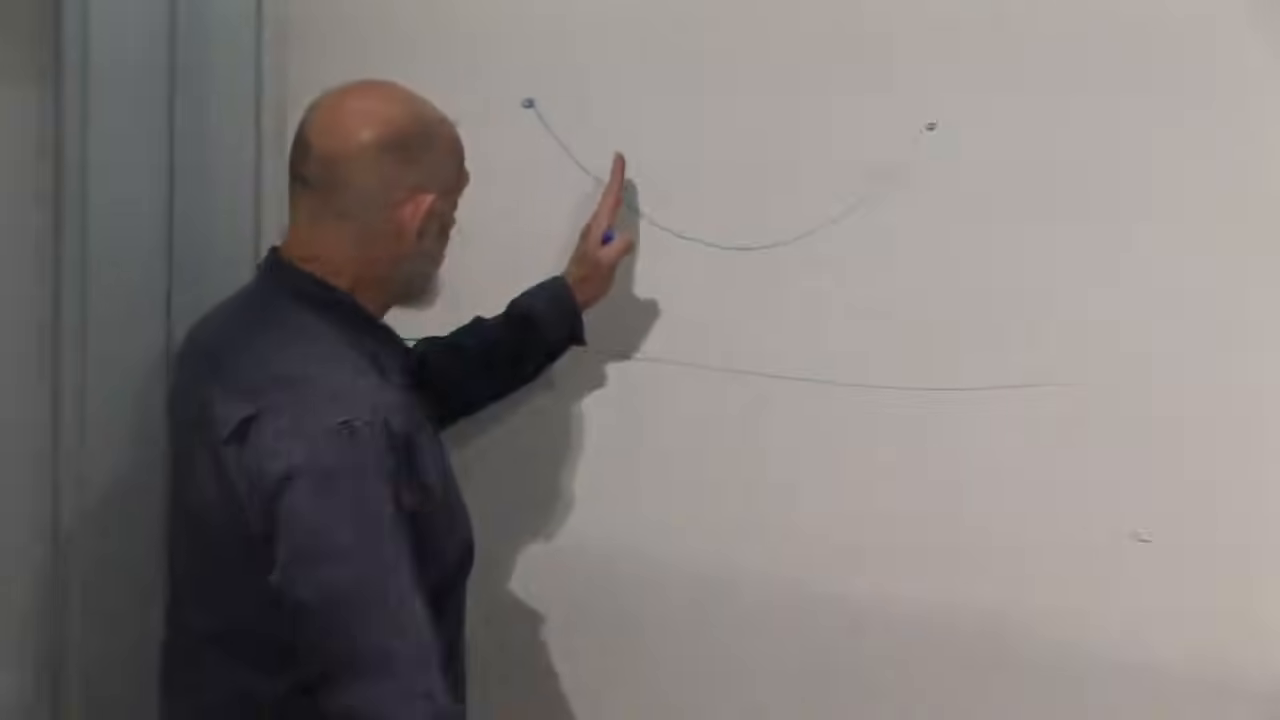
\includegraphics[width=0.76\textwidth]{lecture_03_figure_03.png}
  \caption{Chaîne suspendue entre deux appuis fixes. Sa forme stationnaire est déterminée par l’énergie potentielle de pesanteur totale.}
  \lectureframe{00:30:41}
\end{figure}

Ces exemples ont la même structure : deux extrémités fixes, une fonction qui les relie et une intégrale dont la première variation s’annule. Réduire une telle condition globale à une équation différentielle, c’est résoudre le problème variationnel.

\section{La mécanique comme problème aux limites}

On représente souvent une trajectoire avec le temps à l’horizontale, puisque \(t\) est la variable indépendante. Pourtant, en physique, il est très courant de représenter le temps vers le haut. Une digression rappelle des expériences dans lesquelles des personnes ordonnaient des images allant de la jeunesse à la vieillesse dans le sens associé à leur système d’écriture : les lecteurs de gauche à droite avaient tendance à les disposer de gauche à droite, ceux qui lisaient de droite à gauche faisaient l’inverse, et les personnes habituées à l’écriture verticale les disposaient verticalement. La plaisanterie conclut que les physiciens sont ceux qui insistent pour que le temps s’écoule vers le haut. Nous utiliserons ici l’axe horizontal conventionnel \(t\), car il permet de représenter naturellement \(x(t)\) sous forme de graphe.

Dans la formulation d’un problème à valeur initiale, les données en \(t_0\) sont
\begin{equation}
  x(t_0)=x_0,
  \qquad
  \dot x(t_0)=v_0.
  \label{eq:initial-value-data}
\end{equation}
L’équation de Newton détermine alors l’orbite ultérieure. La formulation variationnelle pose un autre problème : spécifier deux événements aux extrémités,
\begin{equation}
  x(t_0)=x_0,
  \qquad
  x(t_1)=x_1,
  \label{eq:boundary-value-data}
\end{equation}
puis déterminer la trajectoire physique qui les relie. La vitesse initiale n’est plus donnée ; elle fait partie de la solution.

\begin{figure}[htbp]
  \centering
  \includegraphics[width=0.76\textwidth]{lecture_03_figure_09.png}
  \caption{Trajectoire mécanique \(x(t)\). On peut imposer la position et la pente à une extrémité, ou les positions aux deux instants limites.}
  \lectureframe{00:27:41}
\end{figure}

La quantité à rendre stationnaire est l’\emph{action},
\begin{equation}
  A[x]=\int_{t_0}^{t_1}L(x,\dot x,t)\,dt.
  \label{eq:action-one}
\end{equation}
L’intégrande \(L\) est le \emph{lagrangien}. Il peut dépendre de la position, de la vitesse et du temps de manière explicite. Le principe de l’action s’écrit
\begin{equation}
  \delta A=0
  \label{eq:stationary-action}
\end{equation}
pour toutes les petites variations de la trajectoire vérifiant
\begin{equation}
  \delta x(t_0)=\delta x(t_1)=0.
  \label{eq:fixed-endpoint-variations}
\end{equation}
La condition aux extrémités est essentielle : nous comparons des trajectoires voisines qui relient les mêmes deux événements.

\section{Dérivation discrète de l’équation d’Euler--Lagrange}

L’action est une fonctionnelle d’une infinité de valeurs de la trajectoire. Pour rendre sa variation concrète, divisons l’intervalle de temps en pas de longueur
\(\epsilon\),
\begin{equation}
  t_n=t_0+n\epsilon,
  \qquad
  x_n=x(t_n),
  \label{eq:discrete-times}
\end{equation}
et approchons la vitesse sur le \(n\)-ième intervalle par
\begin{equation}
  v_n=\frac{x_{n+1}-x_n}{\epsilon}.
  \label{eq:discrete-velocity}
\end{equation}
L’intégrale devient la somme ordinaire
\begin{equation}
  A_\epsilon
  =\sum_{n=0}^{N-1}
  \epsilon L\left(x_n,\frac{x_{n+1}-x_n}{\epsilon}\right).
  \label{eq:discrete-action}
\end{equation}
Nous utilisons \(n\) comme indice des instants discrétisés afin de garder \(i\) disponible par la suite pour désigner des coordonnées spatiales et des particules.

\begin{figure}[htbp]
  \centering
  \includegraphics[width=0.82\textwidth]{lecture_03_figure_10.png}
  \caption{La trajectoire est remplacée par une suite d’instants discrétisés. La variation d’une hauteur intérieure ne modifie que les deux segments voisins.}
  \lectureframe{00:38:30}
\end{figure}

Faisons varier un point intérieur \(x_n\), en maintenant tous les autres \(x_k\) fixes. Seuls deux termes de la somme dépendent de \(x_n\) :
\begin{align}
  A_\epsilon\big|_{x_n}
  &=
  \epsilon L\left(x_n,\frac{x_{n+1}-x_n}{\epsilon}\right)
  \notag\\
  &\quad+
  \epsilon L\left(x_{n-1},
                  \frac{x_n-x_{n-1}}{\epsilon}\right).
  \label{eq:two-neighbor-terms}
\end{align}
La dérivation donne
\begin{align}
  0=\frac{\partial A_\epsilon}{\partial x_n}
  &=
  \epsilon\frac{\partial L_n}{\partial x_n}
  -\frac{\partial L_n}{\partial v_n}
  +\frac{\partial L_{n-1}}{\partial v_{n-1}}.
  \label{eq:discrete-el-variation}
\end{align}
Les signes opposés s’expliquent simplement par la géométrie. Élever \(x_n\) augmente la pente de l’intervalle précédent et diminue celle de l’intervalle suivant.

\begin{figure}[htbp]
  \centering
  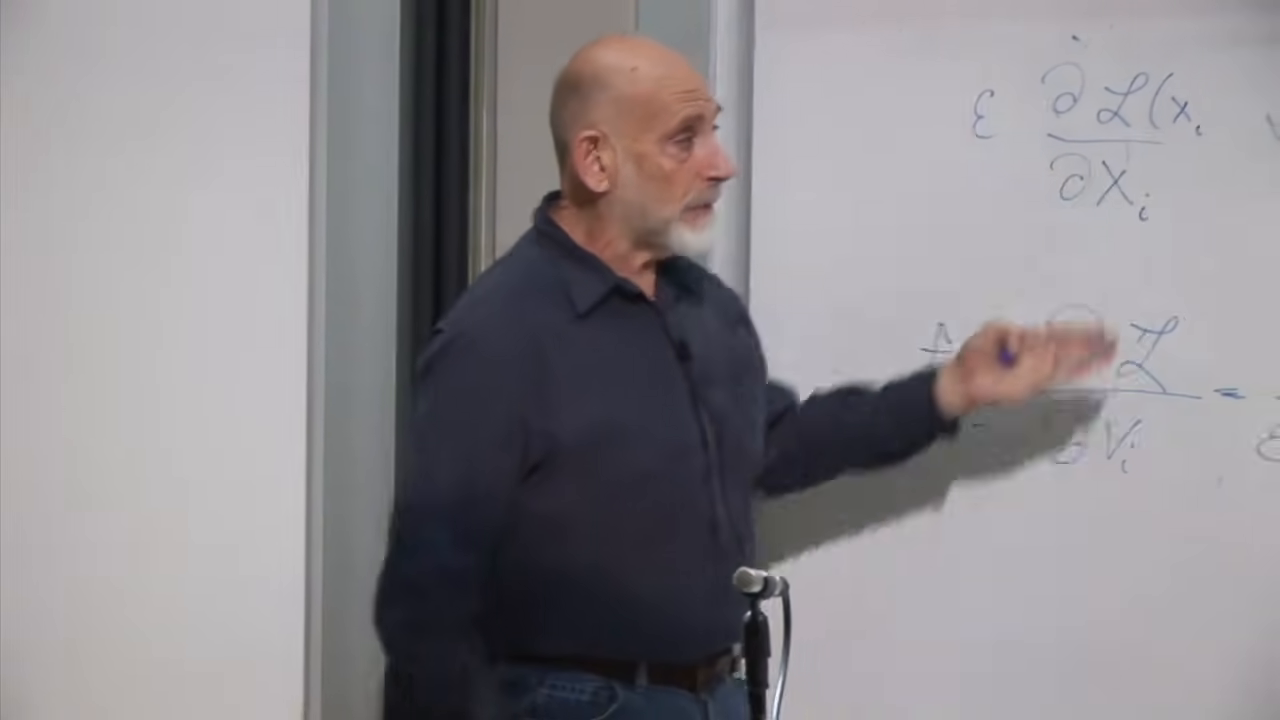
\includegraphics[width=0.74\textwidth]{lecture_03_figure_04.png}
  \caption{La dérivée directe par rapport à la position et les deux contributions des dérivées par rapport à la vitesse provenant des intervalles voisins dans la variation discrète.}
  \lectureframe{00:45:26}
\end{figure}

Réarrangeons l’équation ~\eqref{eq:discrete-el-variation} :
\begin{equation}
  \frac{1}{\epsilon}
  \left(
    \frac{\partial L_n}{\partial v_n}
    -\frac{\partial L_{n-1}}{\partial v_{n-1}}
  \right)
  =
  \frac{\partial L_n}{\partial x_n}.
  \label{eq:discrete-el}
\end{equation}
Le membre de gauche est un quotient de différences entre deux instants voisins. Lorsque \(\epsilon\to0\), la ligne brisée devient une trajectoire lisse et le quotient tend vers une dérivée temporelle :
\begin{equation}
  \boxed{
  \frac{d}{dt}\left(\frac{\partial L}{\partial\dot x}\right)
  =
  \frac{\partial L}{\partial x}}
  .
  \label{eq:euler-lagrange-one}
\end{equation}
C’est l’équation d’Euler--Lagrange.

\begin{figure}[htbp]
  \centering
  \includegraphics[width=0.78\textwidth]{lecture_03_figure_11.png}
  \caption{L’équation d’Euler--Lagrange complète, obtenue en imposant la stationnarité à chaque instant intérieur.}
  \lectureframe{00:49:25}
\end{figure}

Une fois \(L\) spécifié, l’équation ~\eqref{eq:euler-lagrange-one} fonctionne comme une machine : on dérive la fonction donnée et elle renvoie une équation différentielle pour la trajectoire.

\begin{classroomqa}
  \audiencequestion{Le résultat d’Euler--Lagrange est-il valable pour toute fonction de \(x\) et de \(\dot x\) ?\lecturetimestamp{00:49:37--00:50:24}}
  \lecturerresponse{Oui, sous réserve de la régularité nécessaire à l’existence des dérivées. Après avoir renommé sa variable indépendante \(x\) pour lui donner le rôle de \(t\), et sa fonction inconnue \(y(x)\) pour lui donner celui de \(x(t)\), l’exemple de la longueur d’arc prend exactement la même forme. Son équation d’Euler--Lagrange admet des solutions en ligne droite.}
\end{classroomqa}

\section{Retrouver les équations de Newton à partir du lagrangien}

Pour une particule se déplaçant sur une droite dans un potentiel \(V(x)\), posons
\begin{equation}
  L(x,\dot x)=T-V
  =\frac12m\dot x^2-V(x).
  \label{eq:lagrangian-tv-one}
\end{equation}
Le signe moins peut sembler étrange, car l’énergie totale est \(T+V\). Mais le lagrangien n’est pas l’énergie. Il faut vérifier si la machine d’Euler--Lagrange restitue le mouvement correct. On décline une proposition de vote fictif sur le signe : il faut vérifier le résultat, pas le soumettre au vote.

D’abord,
\begin{equation}
  \frac{\partial L}{\partial\dot x}=m\dot x.
  \label{eq:conjugate-momentum-one}
\end{equation}
C’est la quantité de mouvement. Plus généralement, la quantité de mouvement conjuguée à une coordonnée \(q\) est définie par
\begin{equation}
  p_q=\frac{\partial L}{\partial\dot q}.
  \label{eq:conjugate-momentum-general}
\end{equation}
En dérivant l’équation ~\eqref{eq:conjugate-momentum-one} par rapport au temps, on obtient
\(m\ddot x\), tandis que
\begin{equation}
  \frac{\partial L}{\partial x}
  =-\frac{dV}{dx}.
  \label{eq:lagrangian-position-derivative}
\end{equation}
L’équation d’Euler--Lagrange donne donc
\begin{equation}
  m\ddot x=-\frac{dV}{dx}=F(x),
  \label{eq:newton-from-action}
\end{equation}
qui est la deuxième loi de Newton.

\begin{figure}[htbp]
  \centering
  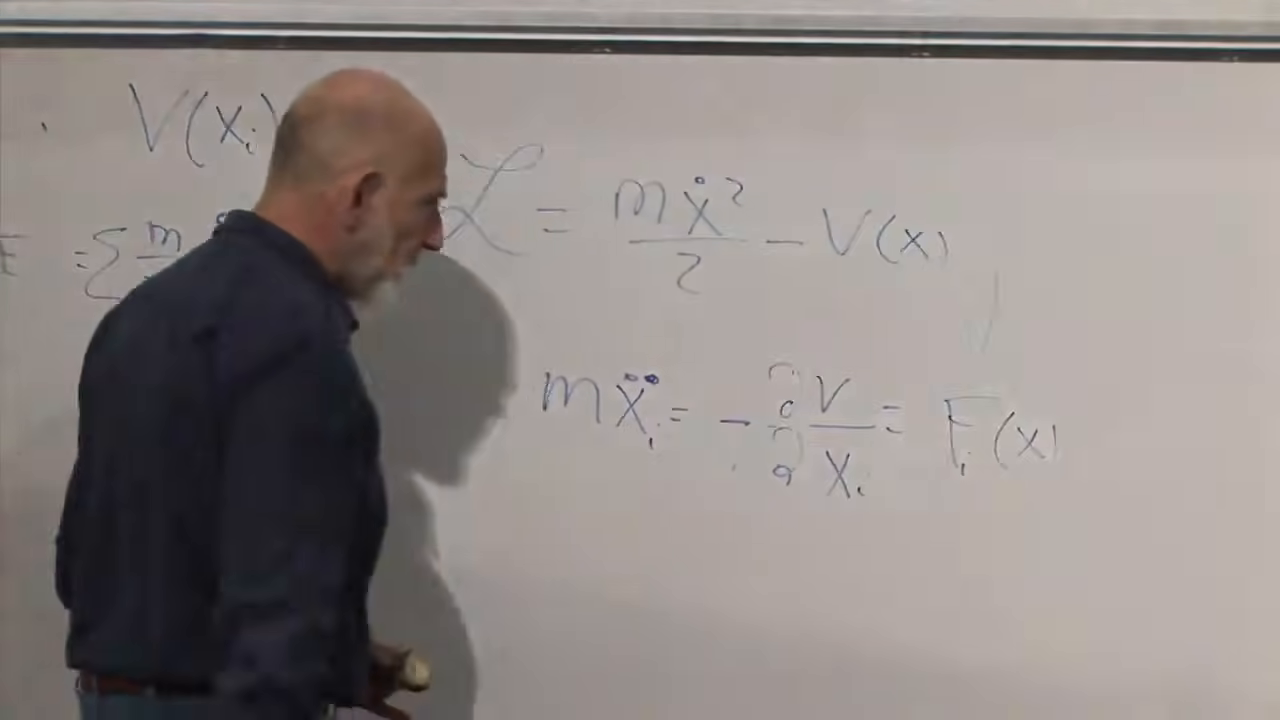
\includegraphics[width=0.80\textwidth]{lecture_03_figure_05.png}
  \caption{Énergie cinétique, énergie potentielle, \(L=T-V\) et expression par composantes de l’équation de Newton retrouvée, réunies au tableau.}
  \lectureframe{00:57:52}
\end{figure}

Pour plusieurs coordonnées \(q_i\),
\begin{equation}
  L(\mathbf q,\dot{\mathbf q})
  =\sum_i\frac12m_i\dot q_i^{\,2}-V(q_1,q_2,\ldots),
  \label{eq:lagrangian-tv-many}
\end{equation}
et il y a une équation pour chaque coordonnée :
\begin{equation}
  \frac{d}{dt}\left(\frac{\partial L}{\partial\dot q_i}\right)
  =\frac{\partial L}{\partial q_i}
  \quad\Longrightarrow\quad
  m_i\ddot q_i=-\frac{\partial V}{\partial q_i}=F_i.
  \label{eq:euler-lagrange-many}
\end{equation}
La trajectoire reste une seule courbe, mais elle se trouve désormais dans un espace des configurations de grande dimension.

\begin{classroomqa}
  \audiencequestion{N’avons-nous pas simplement remonté à rebours la loi de Newton en construisant une fonctionnelle qui restitue le résultat ?\lecturetimestamp{00:58:07--01:00:04}}
  \lecturerresponse{Ce n’est pas la manière la plus féconde d’aborder la question. Le lagrangien donne une spécification compacte du système physique : une fonction de toutes les coordonnées et de toutes les vitesses rassemble toutes ses équations du mouvement. Pour les nouvelles théories, les physiciens proposent généralement une action et en déduisent les équations, au lieu de deviner séparément chacune d’elles.}
\end{classroomqa}

Cette formulation compacte est un avantage. La liberté de choix des coordonnées en est un autre. L’affirmation selon laquelle une ligne est la plus courte ne dépend pas du fait que le plan soit décrit en coordonnées cartésiennes, polaires ou curvilignes. De même, la stationnarité de l’action est indépendante des coordonnées, même si l’expression de \(L\) et les équations obtenues pour ses composantes changent.

\section{Une particule libre vue depuis un manège}

Soient \((x,y)\) des coordonnées cartésiennes inertielles et \((X,Y)\) des coordonnées qui tournent uniformément avec une vitesse angulaire \(\omega\). Avec l’orientation choisie ici,
\begin{align}
  x&=X\cos\omega t+Y\sin\omega t,
  \notag\\
  y&=-X\sin\omega t+Y\cos\omega t.
  \label{eq:rotating-coordinate-map}
\end{align}
L’angle entre les repères est \(\omega t\).

\begin{figure}[htbp]
  \centering
  \includegraphics[width=0.76\textwidth]{lecture_03_figure_12.png}
  \caption{Axes cartésiens inertiels et en rotation uniforme. Les coordonnées tournantes du même point dépendent du temps.}
  \lectureframe{01:06:05}
\end{figure}

Le lagrangien d’une particule libre dans le repère inertiel est
\begin{equation}
  L_{\mathrm{in}}
  =\frac{m}{2}\left(\dot x^2+\dot y^2\right).
  \label{eq:free-inertial-lagrangian}
\end{equation}
Dérivons l’équation ~\eqref{eq:rotating-coordinate-map} et utilisons
\(\sin^2\omega t+\cos^2\omega t=1\). Les termes trigonométriques se combinent pour donner
\begin{align}
  \dot x^2+\dot y^2
  &=
  \dot X^2+\dot Y^2\\
  &\quad+\omega^2(X^2+Y^2)\\
  &\quad+2\omega(Y\dot X-X\dot Y).
  \label{eq:rotating-speed}
\end{align}
Ainsi,
\begin{align}
  L_{\mathrm{rot}}
  &=
  \frac{m}{2}(\dot X^2+\dot Y^2)\\
  &\quad+\frac{m\omega^2}{2}(X^2+Y^2)\\
  &\quad+m\omega(Y\dot X-X\dot Y).
  \label{eq:rotating-lagrangian}
\end{align}

\begin{figure}[htbp]
  \centering
  \includegraphics[width=0.84\textwidth]{lecture_03_figure_13.png}
  \caption{Le lagrangien transformé de la particule libre : l’énergie cinétique ordinaire, un terme quadratique centrifuge et un terme linéaire en vitesse.}
  \lectureframe{01:12:16}
\end{figure}

Le terme quadratique en coordonnées est de la forme \(-V_{\mathrm{fict}}\), où
\begin{equation}
  V_{\mathrm{fict}}
  =-\frac{m\omega^2}{2}(X^2+Y^2).
  \label{eq:centrifugal-potential}
\end{equation}
Il diminue lorsqu’on s’éloigne de l’origine et produit donc la force centrifuge
\(m\omega^2(X,Y)\).

Le dernier terme de l’équation ~\eqref{eq:rotating-lagrangian} est linéaire à la fois en les coordonnées et en les vitesses. L’équation d’Euler--Lagrange donne
\begin{align}
  m\ddot X&=m\omega^2X-2m\omega\dot Y,
  \notag\\
  m\ddot Y&=m\omega^2Y+2m\omega\dot X.
  \label{eq:rotating-equations}
\end{align}
Les termes proportionnels à \(\omega^2\) sont centrifuges ; ceux qui sont proportionnels à la vitesse sont des termes de Coriolis. Dans le plan tournant, l’écriture vectorielle est
\begin{equation}
  \mathbf F_{\mathrm{C}}
  =-2m\,\boldsymbol\omega\times\mathbf v_{\mathrm{rot}},
  \label{eq:coriolis-vector}
\end{equation}
les signes étant inversés si l’on choisit la convention d’orientation opposée.

\begin{figure}[htbp]
  \centering
  \includegraphics[width=0.84\textwidth]{lecture_03_figure_14.png}
  \caption{Équations dans le repère tournant : les termes proportionnels aux coordonnées donnent l’accélération centrifuge, tandis que les termes croisés en vitesse donnent l’accélération de Coriolis.}
  \lectureframe{01:20:20}
\end{figure}

L’essentiel n’est pas que l’algèbre disparaisse. C’est qu’une transformation de coordonnées appliquée à une seule fonction scalaire produit les deux équations couplées et les deux forces fictives.

\begin{classroomqa}
  \audiencequestion{Cette méthode fonctionne-t-elle pour des coordonnées arbitrairement curvilignes ?\lecturetimestamp{01:22:01--01:22:17}}
  \lecturerresponse{Oui. Les nouvelles coordonnées peuvent être curvilignes et même dépendre explicitement du temps, comme c’est le cas des coordonnées tournantes. Réécrivons l’action dans les nouvelles variables et appliquons la même règle d’Euler--Lagrange.}
\end{classroomqa}

\section{Coordonnées polaires et angle cyclique}

En coordonnées polaires usuelles,
\begin{equation}
  x=r\cos\theta,
  \qquad
  y=r\sin\theta.
  \label{eq:polar-map}
\end{equation}
\(r\) et \(\theta\) peuvent varier avec le temps. En dérivant et en additionnant les carrés, on obtient
\begin{equation}
  \dot x^2+\dot y^2
  =\dot r^2+r^2\dot\theta^2.
  \label{eq:polar-speed}
\end{equation}
Pour un potentiel central \(V(r)\),
\begin{equation}
  L
  =\frac{m}{2}\left(\dot r^2+r^2\dot\theta^2\right)-V(r).
  \label{eq:polar-lagrangian}
\end{equation}

\begin{figure}[htbp]
  \centering
  \includegraphics[width=0.80\textwidth]{lecture_03_figure_15.png}
  \caption{Géométrie polaire et décomposition de l’énergie cinétique entre mouvement radial et mouvement angulaire.}
  \lectureframe{01:23:30}
\end{figure}

L’équation radiale est
\begin{equation}
  m\ddot r
  =mr\dot\theta^2-\frac{dV}{dr}.
  \label{eq:radial-equation}
\end{equation}
Le premier terme est la contribution centrifuge dirigée vers l’extérieur, associée au mouvement angulaire propre de la particule.

Pour l’angle,
\begin{equation}
  \frac{d}{dt}\left(\frac{\partial L}{\partial\dot\theta}\right)
  =\frac{\partial L}{\partial\theta}=0,
  \label{eq:theta-el}
\end{equation}
car le potentiel central ne dépend pas explicitement de \(\theta\). On a donc
\begin{equation}
  \frac{d}{dt}\left(mr^2\dot\theta\right)=0,
  \qquad
  mr^2\dot\theta=\ell,
  \label{eq:angular-momentum}
\end{equation}
où \(\ell\) est le moment cinétique conservé.

\begin{figure}[htbp]
  \centering
  \includegraphics[width=0.82\textwidth]{lecture_03_figure_16.png}
  \caption{L’équation d’Euler--Lagrange pour la coordonnée angulaire a un second membre nul, ce qui met en évidence la conservation de \(mr^2\dot\theta\).}
  \lectureframe{01:29:25}
\end{figure}

L’équation angulaire donne
\begin{equation}
  \dot\theta=\frac{\ell}{mr^2}.
  \label{eq:theta-dot-angular-momentum}
\end{equation}
En substituant dans l’équation ~\eqref{eq:radial-equation}, il reste une seule équation pour \(r\) :
\begin{equation}
  m\ddot r
  =\frac{\ell^2}{mr^3}-\frac{dV}{dr}.
  \label{eq:effective-radial-equation}
\end{equation}

Une coordonnée absente de \(L\) est traditionnellement dite \emph{cyclique}, même si ce n’est pas un angle. Si \(q\) est cyclique, alors
\begin{equation}
  \frac{\partial L}{\partial q}=0
  \quad\Longrightarrow\quad
  \frac{d}{dt}\left(\frac{\partial L}{\partial\dot q}\right)=0.
  \label{eq:cyclic-conservation}
\end{equation}
sa quantité de mouvement conjuguée est conservée. On entrevoit ainsi le lien général entre symétrie et loi de conservation.

\section{Questions sur le sens, l’énergie et la portée}

Les questions qui suivent mettent en évidence où réside le contenu profond du formalisme.

\begin{classroomqa}
  \audiencequestion{Existe-t-il une raison indépendante de parvenir au lagrangien, au-delà du fait qu’il donne les bonnes équations classiques ?\lecturetimestamp{01:33:25--01:35:07}}
  \lecturerresponse{Historiquement, plus d’un siècle de mécanique classique a montré que les particules, les ondes et les champs électromagnétiques pouvaient tous être décrits sous cette forme. Au niveau classique, ce succès accumulé est un fait empirique sur la manière dont les lois s’organisent. L’explication plus profonde vient de la mécanique quantique et sera abordée plus tard.}
\end{classroomqa}

\begin{classroomqa}
  \audiencequestion{Dans le lagrangien du repère tournant, peut-on attribuer au terme linéaire en vitesse une énergie cinétique ou potentielle ordinaire ?\lecturetimestamp{01:35:08--01:36:23}}
  \lecturerresponse{Non. La quantité conservée associée aux translations temporelles s’obtient par la construction hamiltonienne ; on ne peut pas interpréter chaque terme de \(L\) comme une énergie cinétique ou potentielle. Dans l’équation ~\eqref{eq:rotating-lagrangian}, le terme linéaire en vitesse s’élimine de \(\sum_a\dot q_a\,\partial L/\partial\dot q_a-L\). Le formalisme hamiltonien organisera cela de façon systématique.}
\end{classroomqa}

En effet, puisque \(L_{\mathrm{rot}}\) ne dépend pas explicitement du temps,
\begin{equation}
  \begin{aligned}
    H_{\mathrm{rot}}
    &=\dot X\frac{\partial L}{\partial\dot X}
     +\dot Y\frac{\partial L}{\partial\dot Y}-L\\
    &=\frac{m}{2}(\dot X^2+\dot Y^2)
     -\frac{m\omega^2}{2}(X^2+Y^2)
  \end{aligned}
  \label{eq:rotating-hamiltonian-preview}
\end{equation}
est conservée. C’est l’intégrale de Jacobi dans le repère tournant, et non la même valeur numérique de l’énergie que celle attribuée par l’observateur inertiel. Un changement de coordonnées dépendant du temps ne préserve pas nécessairement la forme numérique de l’énergie.

\begin{classroomqa}
  \audiencequestion{Que se passe-t-il si la trajectoire courbe est due à la gravité ?\lecturetimestamp{01:36:30--01:37:10}}
  \lecturerresponse{Pour la gravitation newtonienne, il suffit d’utiliser \(V(r)=-GMm/r\) dans le lagrangien à force centrale. L’espace-temps courbe relève de la relativité générale et n’est pas pris en compte ici.}
\end{classroomqa}

\begin{classroomqa}
  \audiencequestion{Le potentiel centrifuge et l’énergie qui lui est associée sont-ils simplement fictifs ?\lecturetimestamp{01:37:13--01:40:14}}
  \lecturerresponse{Un observateur sur la plateforme tournante mesure les forces effectives et peut utiliser de manière cohérente la quantité conservée dans le repère tournant. Le terme \emph{fictif} signifie que ces termes viennent d’une description non inertielle, et non que leurs effets observés sont imaginaires. L’énergie elle-même n’est pas invariante sous un changement général de coordonnées dépendant du temps.}
\end{classroomqa}

\begin{classroomqa}
  \audiencequestion{Dans quelle direction pointe la force de Coriolis, qui dépend de la vitesse ?\lecturetimestamp{01:40:22--01:42:36}}
  \lecturerresponse{Elle est perpendiculaire à la vitesse dans le repère tournant ; sa norme est proportionnelle à la vitesse et à la vitesse angulaire du repère. Dans le plan, les composantes de \(\dot X\) et de \(\dot Y\) s’échangent avec des signes opposés, comme dans l’équation ~\eqref{eq:rotating-equations}.}
\end{classroomqa}

\clearpage
\begin{figure}[htbp]
  \centering
  \includegraphics[width=0.76\textwidth]{lecture_03_figure_17.png}
  \caption{Structure des composantes croisées en vitesse : la force de Coriolis est perpendiculaire à la vitesse dans le repère tournant.}
  \lectureframe{01:41:40}
\end{figure}

\begin{classroomqa}
  \audiencequestion{Le lagrangien de départ doit-il être écrit dans un repère inertiel ?\lecturetimestamp{01:42:37--01:44:00}}
  \lecturerresponse{Pour une particule libre ordinaire, la loi de Newton dans un repère inertiel fournit la forme initiale simple \(m(\dot x^2+\dot y^2)/2\). Une fois cette loi physique connue, on peut transformer l’action vers n’importe quel autre système de coordonnées. Il ne faut pas supposer indépendamment que la même formule simple de l’énergie cinétique s’applique dans un repère tournant.}
\end{classroomqa}

On trouve le même type de terme linéaire en vitesse pour une particule chargée dans un champ magnétique :
\begin{equation}
  L_{\mathrm{em}}
  =\frac12m\mathbf v^2
   +q\mathbf A(\mathbf r,t)\cdot\mathbf v
   -q\phi(\mathbf r,t).
  \label{eq:electromagnetic-lagrangian}
\end{equation}
Pour un champ magnétique uniforme perpendiculaire au plan, la jauge symétrique \(\mathbf A=\tfrac12\mathbf B\times\mathbf r\) produit un terme proportionnel à \(X\dot Y-Y\dot X\), qui a la même structure algébrique que le terme de Coriolis.

\begin{figure}[htbp]
  \centering
  \includegraphics[width=0.82\textwidth]{lecture_03_figure_18.png}
  \caption{Le terme linéaire en vitesse du repère tournant, qui motive la comparaison avec une particule chargée dans un champ magnétique uniforme.}
  \lectureframe{01:44:40}
\end{figure}

\begin{classroomqa}
  \audiencequestion{La fonction susceptible de jouer le rôle de lagrangien est-elle soumise à des contraintes autres que la régularité ?\lecturetimestamp{01:44:46--01:45:06}}
  \lecturerresponse{Oui, mais les contraintes pertinentes nécessitent un cadre plus élaboré, qui n’a pas encore été présenté ; nous les réserverons pour plus tard. Pour l’instant, l’idée centrale est de voir comment un lagrangien proposé engendre des équations et des lois de conservation.}
\end{classroomqa}

Les équations dans le repère tournant admettent aussi un mouvement circulaire : un point fixe dans le repère inertiel est vu depuis le manège comme décrivant un cercle autour de l’origine tournante. L’analogie magnétique explique alors pourquoi une particule chargée peut effectuer un mouvement cyclotron circulaire.

\begin{classroomqa}
  \audiencequestion{Une particule chargée resterait-elle sur ce cercle, ou le rayonnement ferait-il s’effondrer son orbite ?\lecturetimestamp{01:46:11--01:47:21}}
  \lecturerresponse{Les équations pour la particule seule dont il est question ici ne tiennent pas compte du rayonnement. Dès lors qu’on inclut le couplage au champ électromagnétique et la réaction de rayonnement, une charge classique accélérée peut rayonner. Le rayonnement est donc un effet physique supplémentaire, qui ne contredit pas l’orbite décrite par les équations tronquées.}
\end{classroomqa}

\begin{classroomqa}
  \audiencequestion{Quel est le rapport avec les ouragans ?
  \lecturetimestamp{01:47:30--01:47:50}}
  \lecturerresponse{Les mouvements atmosphériques à grande échelle se produisent sur la Terre en rotation ; les effets de Coriolis y sont donc importants. Une dérivation correcte relève de la météorologie et ne sera pas tentée ici.}
\end{classroomqa}

\begin{classroomqa}
  \audiencequestion{Le cadre de l’action est-il censé couvrir toutes les lois physiques, et que signifierait une véritable exception ?\lecturetimestamp{01:47:57--01:49:01}}
  \lecturerresponse{Toutes les théories fondamentales fermées connues dans le cadre de cette discussion peuvent s’organiser autour d’une action : les particules newtoniennes, les champs de Maxwell, la relativité générale et le Modèle standard. Les contre-exemples apparents, comme la traînée visqueuse, surviennent lorsqu’on omet les degrés de liberté de l’environnement. Si l’on élargit le système pour y inclure le fluide ou le bain microscopique, la description fondamentale s’inscrit de nouveau dans ce cadre. Une exception véritablement fondamentale constituerait donc une découverte majeure.}
\end{classroomqa}
\chapter{Symétrie et lois de conservation}

\lectureoverview{L’action stationnaire et les équations d’Euler--Lagrange constituent une moitié du cœur de la mécanique classique ; la formulation hamiltonienne en est l’autre. Nous allons développer suffisamment cette première moitié pour mettre au jour un schéma profond : toute symétrie continue d’un lagrangien produit une grandeur conservée. Nous découvrirons ce schéma à travers les translations et les rotations, le démontrerons pour une transformation infinitésimale générale, puis examinerons avec soin les cas où le raisonnement s’applique et ceux où il ne s’applique pas.}

\section{Le minimum de mathématiques qui explique la physique}

Les expressions déjà inscrites au tableau ressemblent peut-être un peu à l’équation de Schrödinger, mais ce n’est pas le sujet de ce soir. Nous allons parler de symétrie et de conservation. Il est impossible d’expliquer honnêtement leur lien sans équations. Les équations sont élémentaires ; l’essentiel est de les agencer de façon à faire apparaître la structure. Scientific American peut nommer le résultat, mais nous voulons ici établir le minimum de mathématiques nécessaire pour le déduire comme le feraient des physiciens.

Introduisons un petit paramètre \(\epsilon\). Nous conservons les termes proportionnels à \(\epsilon\) et négligeons ceux en \(O(\epsilon^2)\). C’est une façon abrégée de désigner un raisonnement par passage à la limite, et non d’affirmer que le carré d’un nombre réel non nul est littéralement nul. Pour une fonction ordinaire \(f(x,y)\),
\begin{equation}
  \delta f
  =\frac{\partial f}{\partial x}\,\delta x
   +\frac{\partial f}{\partial y}\,\delta y
   +O(\epsilon^2),
  \label{eq:first-variation-f}
\end{equation}
où \(\delta x\) et \(\delta y\) sont toutes deux proportionnelles à \(\epsilon\). Le symbole \(\delta f\) désigne la variation de \(f\), et non le produit d’un nombre appelé \(\delta\) par \(f\). Un point stationnaire vérifie
\begin{equation}
  \delta f=0
  \qquad\hbox{to first order.}
  \label{eq:stationary-f}
\end{equation}

Pour une trajectoire mécanique \(q_i(t)\), la quantité analogue est l’action
\begin{equation}
  S[q]=\int_{t_1}^{t_2}L(q,\dot q,t)\,dt.
  \label{eq:action-l4}
\end{equation}
La variation de la trajectoire à extrémités fixes donne
\begin{equation}
  \delta S
  =\int_{t_1}^{t_2}dt\,
   \sum_i\left(
     \frac{\partial L}{\partial q_i}\,\delta q_i
     +\frac{\partial L}{\partial\dot q_i}\,\delta\dot q_i
   \right).
  \label{eq:action-variation-l4}
\end{equation}
Les deux termes apparaissent parce qu’une variation de trajectoire modifie à la fois sa position et sa vitesse. L’intégration par parties, associée à
\(\delta q_i(t_1)=\delta q_i(t_2)=0\), transforme \(\delta S=0\) en
\begin{equation}
  \frac{d}{dt}\left(\frac{\partial L}{\partial\dot q_i}\right)
  -\frac{\partial L}{\partial q_i}=0.
  \label{eq:el-l4}
\end{equation}

\begin{figure}[htbp]
  \centering
  \includegraphics[width=0.76\textwidth]{lecture_04_figure_05.png}
  \caption{L’équation d’Euler--Lagrange, rappelée comme point de départ pour étudier symétrie et conservation.}
  \lectureframe{00:09:00}
\end{figure}

L’expression correcte est \emph{action stationnaire}, et non nécessairement action minimale. Nous reviendrons sur cette distinction vers la fin.

\section{Coordonnées généralisées et quantité de mouvement conjuguée}

Les positions cartésiennes ne suffisent pas à décrire la mécanique générale. Les coordonnées peuvent être des positions de particules, des angles, des variables collectives ou des amplitudes de champ ; nous les appelons donc \(q_i\). Un lagrangien est une description condensée de la dynamique. Même le Modèle standard, écrit sans notation très condensée, occupe environ une page ; écrire une équation du mouvement distincte pour chaque composante de champ en demanderait beaucoup plus. La fonction unique \(L\) rassemble toutes ces informations.

La quantité de mouvement conjuguée à \(q_i\) est
\begin{equation}
  p_i=\frac{\partial L}{\partial\dot q_i}.
  \label{eq:canonical-momentum-l4}
\end{equation}
C’est pourquoi on appelle traditionnellement les coordonnées généralisées des \(q\) ; les quantités de mouvement correspondantes sont des \(p\), ce qui nous donne nos \(p\) et nos \(q\). Avec cette notation, l’équation ~\eqref{eq:el-l4} devient
\begin{equation}
  \dot p_i=\frac{\partial L}{\partial q_i}.
  \label{eq:momentum-el-l4}
\end{equation}

Pour la particule familière à une dimension,
\begin{equation}
  L=\frac{m\dot x^2}{2}-V(x),
  \qquad
  \frac{\partial L}{\partial\dot x}=m\dot x,
  \label{eq:particle-momentum-l4}
\end{equation}
la quantité de mouvement conjuguée est donc la quantité de mouvement ordinaire.

\begin{figure}[htbp]
  \centering
  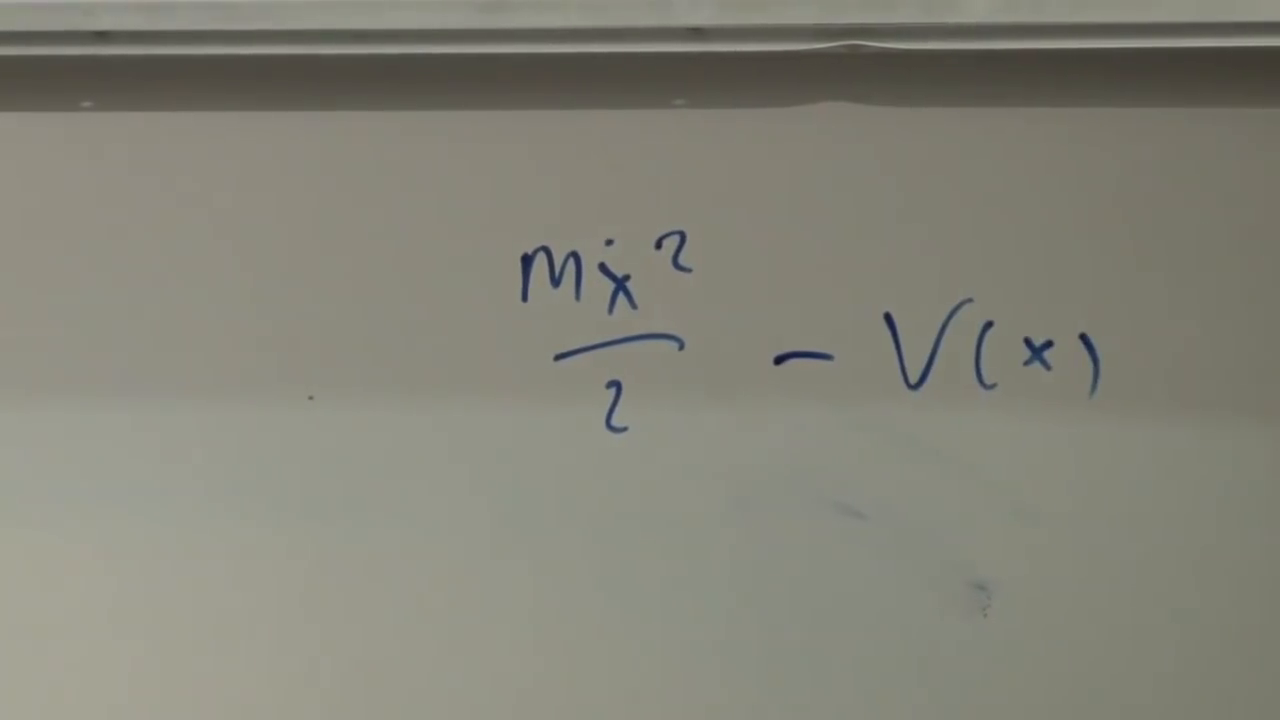
\includegraphics[width=0.72\textwidth]{lecture_04_figure_02.png}
  \caption{Le lagrangien égal à l’énergie cinétique moins l’énergie potentielle, utilisé pour identifier la quantité de mouvement conjuguée à \(m\dot x\).}
  \lectureframe{00:14:48}
\end{figure}

Si \(q_i\) n’apparaît pas dans \(L\), alors \(\dot p_i=0\). C’est la démarche familière qui consiste à invoquer une coordonnée cyclique pour obtenir une loi de conservation. Le lien véritable est plus général, et il est utile de le découvrir à travers des exemples avant de le démontrer.

\section{Découvrir des lois de conservation avant de les expliquer}

\subsection{Deux coordonnées et un potentiel dépendant de leur écart}

Prenons les deux masses égales à l’unité et considérons
\begin{equation}
  L=\frac{\dot q_1^{\,2}+\dot q_2^{\,2}}{2}-V(q_1-q_2).
  \label{eq:separation-lagrangian}
\end{equation}
On peut se représenter deux particules sur une droite. Leur interaction ne dépend que de leur écart.

\begin{figure}[htbp]
  \centering
  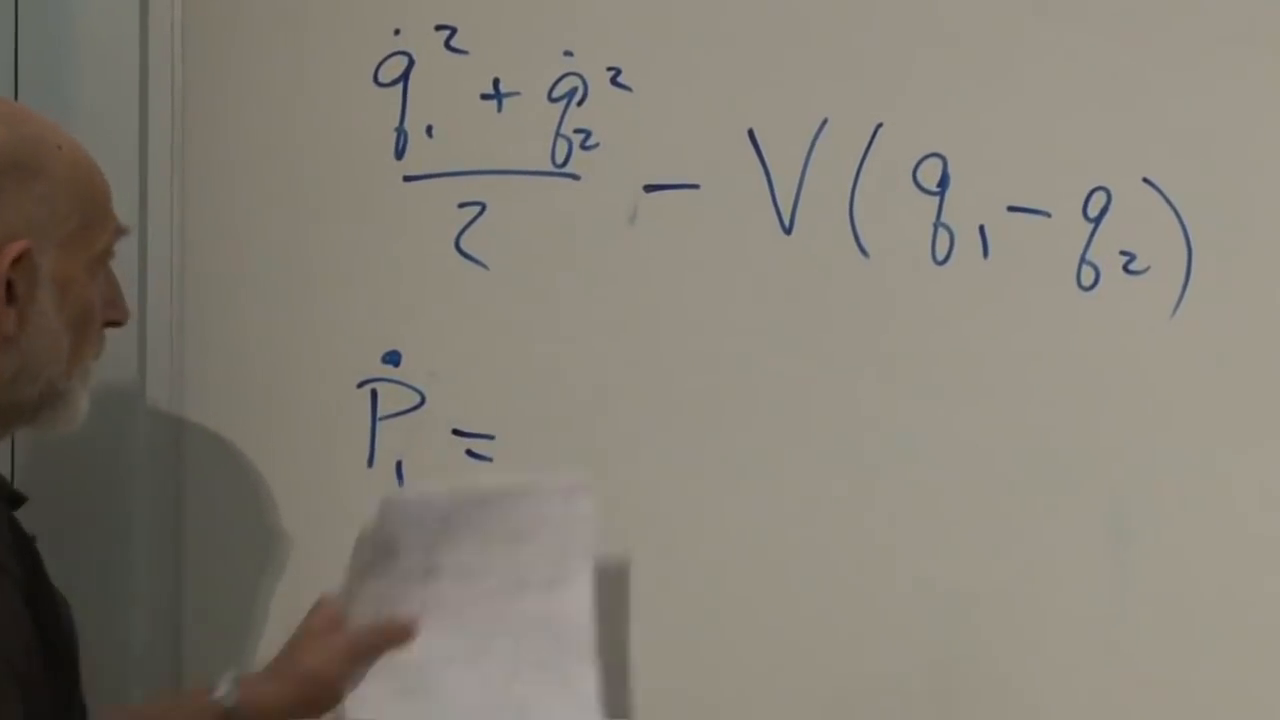
\includegraphics[width=0.78\textwidth]{lecture_04_figure_03.png}
  \caption{Le lagrangien à deux coordonnées et le début de la première équation pour les quantités de mouvement.}
  \lectureframe{00:18:56}
\end{figure}

Notons \(V'\) la dérivée par rapport à l’argument de \(V\) ; on obtient
\begin{align}
  \dot p_1&=-V'(q_1-q_2),
  \notag\\
  \dot p_2&=+V'(q_1-q_2).
  \label{eq:separation-momentum-equations}
\end{align}
Le signe de la seconde équation est opposé parce qu’une augmentation de \(q_2\) diminue \(q_1-q_2\).

\begin{classroomqa}
  \audiencequestion{La première équation pour la quantité de mouvement doit-elle contenir \(V'\), et d’où vient son signe moins ?
  \lecturetimestamp{00:20:52--00:21:35}}
  \lecturerresponse{L’équation d’Euler--Lagrange indique que
  \(\dot p_1=\partial L/\partial q_1\), et non que le lagrangien est nul.
  Puisque \(L=T-V\), la dérivation par rapport à \(q_1\) donne
  \(-V'\). La dérivation par rapport à \(q_2\) ajoute un autre signe moins, provenant de \(q_1-q_2\) ; la seconde équation contient donc \(+V'\).}
\end{classroomqa}

\begin{figure}[htbp]
  \centering
  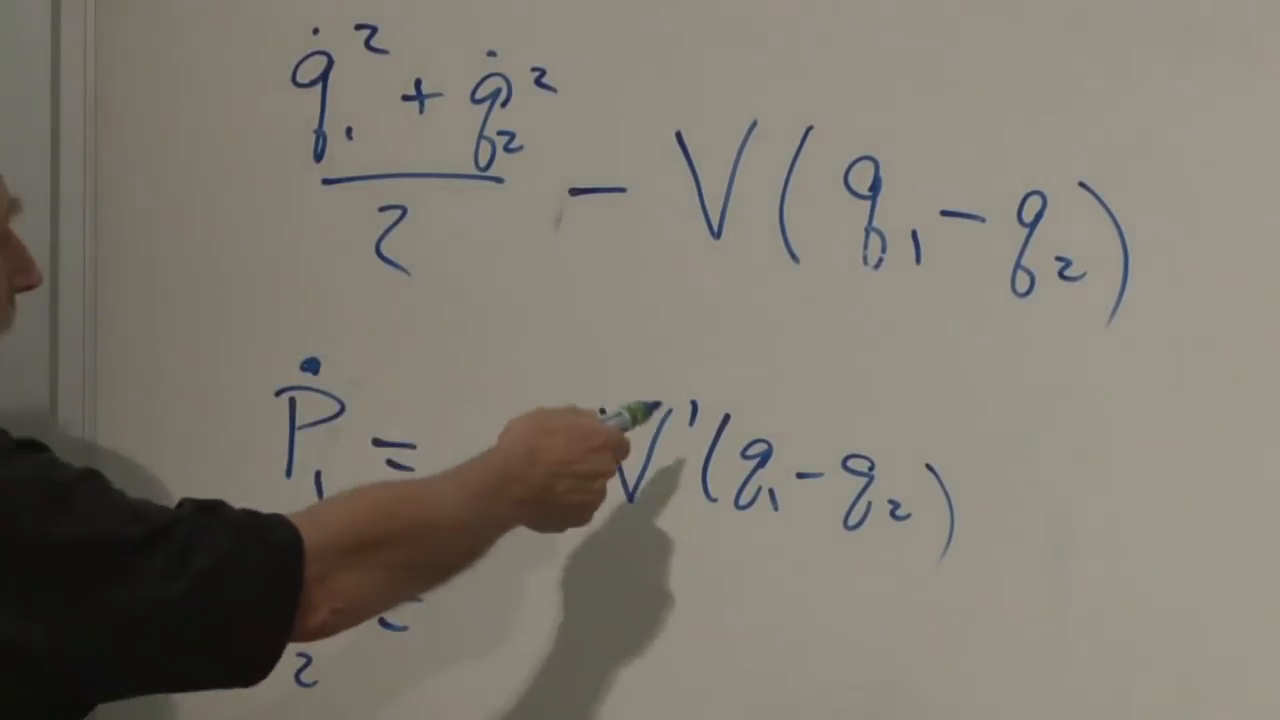
\includegraphics[width=0.78\textwidth]{lecture_04_figure_04.png}
  \caption{La dérivée dont le signe est crucial dans l’équation de \(p_1\) ; l’équation de \(p_2\) reçoit le signe opposé.}
  \lectureframe{00:20:41}
\end{figure}

En additionnant les équations ~\eqref{eq:separation-momentum-equations}, on obtient
\begin{equation}
  \frac{d}{dt}(p_1+p_2)=0.
  \label{eq:total-p-conserved}
\end{equation}
Nous avons trouvé une grandeur conservée, sans encore expliquer pourquoi elle existe.

\subsection{Une combinaison linéaire moins évidente}

Posons maintenant
\begin{equation}
  L=\frac{\dot q_1^{\,2}+\dot q_2^{\,2}}{2}
    -V(Aq_1+Bq_2),
  \label{eq:ab-lagrangian}
\end{equation}
où \(A\) et \(B\) sont des constantes. Alors
\begin{align}
  \dot p_1&=-A\,V'(Aq_1+Bq_2),
  \notag\\
  \dot p_2&=-B\,V'(Aq_1+Bq_2).
  \label{eq:ab-momentum-equations}
\end{align}
En multipliant la première équation par \(B\), la seconde par \(A\), puis en soustrayant, on élimine la force :
\begin{equation}
  \frac{d}{dt}(Bp_1-Ap_2)=0.
  \label{eq:ab-conserved}
\end{equation}

\begin{figure}[htbp]
  \centering
  \includegraphics[width=0.78\textwidth]{lecture_04_figure_06.png}
  \caption{Les équations pondérées pour les quantités de mouvement, dont les termes de force s’annulent dans \(Bp_1-Ap_2\).}
  \lectureframe{00:24:20}
\end{figure}

\begin{classroomqa}
  \audiencequestion{Quelle interprétation physique peut-on donner à des constantes telles que \(A\) et \(B\) ?
  \lecturetimestamp{00:25:09--00:30:15}}
  \lecturerresponse{Considérons deux particules de masses \(m\) et \(M\) :
  \[
    L=\frac{m\dot X^2}{2}+\frac{M\dot Y^2}{2}-V(X-Y).
  \]
  Faisons le changement d’échelle \(Q_1=\sqrt m\,X\) et \(Q_2=\sqrt M\,Y\). Le terme cinétique devient \((\dot Q_1^2+\dot Q_2^2)/2\), tandis que le potentiel dépend de \(Q_1/\sqrt m-Q_2/\sqrt M\). Ainsi, des masses inégales deviennent naturellement des coefficients dans une combinaison linéaire. Remplacer \(Q_2\) par \(-Q_2\) transforme le signe moins affiché en signe plus, sans modifier le terme cinétique quadratique.}
\end{classroomqa}

\begin{figure}[htbp]
  \centering
  \includegraphics[width=0.82\textwidth]{lecture_04_figure_07.png}
  \caption{Les coordonnées pondérées par les masses simplifient l’énergie cinétique, tandis que les facteurs de masse se retrouvent dans le potentiel.}
  \lectureframe{00:28:40}
\end{figure}

\begin{classroomqa}
  \audiencequestion{Cela montre-t-il qu’une grandeur conservée peut exister sans coordonnée cyclique ?
  \lecturetimestamp{00:31:13--00:31:58}}
  \lecturerresponse{Dans les variables écrites ici, il n’y a pas de coordonnée cyclique \emph{évidente}. Un changement de variables peut en faire apparaître une, mais ce n’est pas la façon utile d’aborder le problème que de la rechercher. L’argument de symétrie identifiera directement la combinaison conservée.}
\end{classroomqa}

\section{Ce que nous entendons par symétrie}

\subsection{Translations}

Partons d’une particule libre de masse unité,
\begin{equation}
  L=\frac{\dot q^2}{2}.
  \label{eq:free-unit-l4}
\end{equation}
Translatons chaque point de son histoire de la même constante :
\begin{equation}
  q'(t)=q(t)+\epsilon.
  \label{eq:free-translation}
\end{equation}
Comme \(\epsilon\) ne dépend pas du temps, \(\dot q'=\dot q\), et donc
\(\delta L=0\). Cette invariance est une symétrie de translation.

Il existe deux descriptions équivalentes. Dans la description passive, on déplace l’origine des coordonnées en laissant l’objet fixe. Dans la description active, on garde les axes fixes et on déplace l’objet. Le langage actif sera moins source de confusion : déplaçons la configuration physique et demandons-nous si \(L\) s’en aperçoit.

Pour l’équation ~\eqref{eq:separation-lagrangian}, translatons les deux coordonnées :
\begin{equation}
  \delta q_1=\epsilon,
  \qquad
  \delta q_2=\epsilon.
  \label{eq:common-translation}
\end{equation}
Les vitesses restent inchangées, tout comme \(q_1-q_2\).

\begin{figure}[htbp]
  \centering
  \includegraphics[width=0.78\textwidth]{lecture_04_figure_08.png}
  \caption{Une translation commune laisse inchangé l’écart entre deux coordonnées.}
  \lectureframe{00:35:30}
\end{figure}

Pour l’équation ~\eqref{eq:ab-lagrangian}, considérons la transformation moins évidente
\begin{equation}
  \delta q_1=B\epsilon,
  \qquad
  \delta q_2=-A\epsilon.
  \label{eq:ab-transformation}
\end{equation}
Là encore, les vitesses ne changent pas, tandis que
\begin{equation}
  \delta(Aq_1+Bq_2)=AB\epsilon-BA\epsilon=0.
  \label{eq:ab-invariant-argument}
\end{equation}
Cette transformation est donc une symétrie.

\begin{figure}[htbp]
  \centering
  \includegraphics[width=0.80\textwidth]{lecture_04_figure_09.png}
  \caption{La translation asymétrique qui préserve \(Aq_1+Bq_2\).}
  \lectureframe{00:40:20}
\end{figure}

\begin{classroomqa}
  \audiencequestion{Les coefficients représentent-ils les masses, de sorte que la grandeur conservée devienne la quantité de mouvement ordinaire du centre de masse ?
  \lecturetimestamp{00:42:25--00:42:45}}
  \lecturerresponse{Oui. Dans les variables pondérées par les masses, la symétrie et la combinaison conservée semblent asymétriques. En revenant à \(X\) et \(Y\), on retrouve la translation simultanée ordinaire et la quantité de mouvement totale.}
\end{classroomqa}

\subsection{Rotations}

Considérons une particule dans le plan,
\begin{equation}
  L=\frac{m}{2}(\dot x^2+\dot y^2)-V(x^2+y^2).
  \label{eq:central-lagrangian-l4}
\end{equation}
Il s’agit d’un potentiel central. Comparons deux systèmes de coordonnées fixes, tournés l’un par rapport à l’autre ; les axes ne tournent pas au cours du temps. En choisissant une orientation cohérente,
\begin{align}
  x'&=x\cos\theta+y\sin\theta,
  \notag\\
  y'&=-x\sin\theta+y\cos\theta.
  \label{eq:finite-rotation-l4}
\end{align}

\begin{figure}[htbp]
  \centering
  \includegraphics[width=0.82\textwidth]{lecture_04_figure_10.png}
  \caption{Un lagrangien à potentiel central et deux repères cartésiens fixes liés par une rotation.}
  \lectureframe{00:45:40}
\end{figure}

Posons \(\theta=\epsilon\) et conservons les termes du premier ordre :
\begin{equation}
  \cos\epsilon=1+O(\epsilon^2),
  \qquad
  \sin\epsilon=\epsilon+O(\epsilon^3).
  \label{eq:small-angle-l4}
\end{equation}
La rotation infinitésimale s’écrit
\begin{align}
  \delta x&=y\epsilon,
  &\delta y&=-x\epsilon,
  \notag\\
  \delta\dot x&=\dot y\epsilon,
  &\delta\dot y&=-\dot x\epsilon.
  \label{eq:infinitesimal-rotation-l4}
\end{align}

\begin{figure}[htbp]
  \centering
  \includegraphics[width=0.82\textwidth]{lecture_04_figure_11.png}
  \caption{La rotation infinitésimale des coordonnées et des vitesses.}
  \lectureframe{00:49:50}
\end{figure}

À la différence d’une translation, la variation de \(x\) dépend de \(y\), et celle de \(y\) dépend de \(x\). Pourtant,
\begin{align}
  \delta(x^2+y^2)
  &=2x\,\delta x+2y\,\delta y=0,
  \notag\\
  \delta(\dot x^2+\dot y^2)
  &=2\dot x\,\delta\dot x+2\dot y\,\delta\dot y=0.
  \label{eq:rotation-invariants-l4}
\end{align}
Les termes de potentiel et d’énergie cinétique sont tous deux invariants.

\begin{figure}[htbp]
  \centering
  \includegraphics[width=0.76\textwidth]{lecture_04_figure_12.png}
  \caption{L’annulation au premier ordre qui démontre l’invariance du rayon au carré par rotation.}
  \lectureframe{00:53:20}
\end{figure}

\section{Théorème général de conservation}

Les exemples de translation et de rotation ont la même forme. Considérons une transformation continue infinitésimale
\begin{equation}
  \delta q_i=\epsilon f_i(q),
  \qquad
  \delta\dot q_i=\frac{d}{dt}\delta q_i,
  \label{eq:general-infinitesimal-symmetry}
\end{equation}
où \(\epsilon\) est indépendant du temps et où \(f_i\) peut dépendre de toutes les coordonnées.

\begin{figure}[htbp]
  \centering
  \includegraphics[width=0.78\textwidth]{lecture_04_figure_13.png}
  \caption{Un champ général de déplacements infinitésimaux \(\delta q_i=\epsilon f_i(q)\).}
  \lectureframe{00:56:00}
\end{figure}

La variation du lagrangien au premier ordre est
\begin{equation}
  \delta L
  =\sum_i\left(
    \frac{\partial L}{\partial q_i}\delta q_i
    +\frac{\partial L}{\partial\dot q_i}\delta\dot q_i
  \right).
  \label{eq:delta-l-general}
\end{equation}

\begin{figure}[htbp]
  \centering
  \includegraphics[width=0.84\textwidth]{lecture_04_figure_14.png}
  \caption{Les deux contributions à \(\delta L\) : la variation des coordonnées et celle des vitesses.}
  \lectureframe{01:02:30}
\end{figure}

Restreignons-nous maintenant à une trajectoire physique, qui vérifie donc les équations d’Euler--Lagrange. En utilisant
\begin{equation}
  \frac{\partial L}{\partial\dot q_i}=p_i,
  \qquad
  \frac{\partial L}{\partial q_i}=\dot p_i,
  \label{eq:el-substitution-l4}
\end{equation}
on trouve
\begin{align}
  \delta L
  &=\sum_i\left(\dot p_i\,\delta q_i
                +p_i\,\delta\dot q_i\right)
  \notag\\
  &=\frac{d}{dt}\sum_i p_i\delta q_i
  =\epsilon\frac{d}{dt}\sum_i p_i f_i(q).
  \label{eq:noether-derivation-l4}
\end{align}
L’étape centrale consiste simplement à appliquer la règle du produit.

Si la transformation est une symétrie, alors \(\delta L=0\). Comme \(\epsilon\) est un facteur constant arbitraire,
\begin{equation}
  \boxed{
  \frac{d\mathcal Q}{dt}=0,
  \qquad
  \mathcal Q=\sum_i p_i f_i(q)}
  .
  \label{eq:noether-charge-l4}
\end{equation}
C’est le cœur, en mécanique classique, du théorème de Noether pour les symétries ponctuelles exactes et indépendantes du temps.

\begin{figure}[htbp]
  \centering
  \includegraphics[width=0.84\textwidth]{lecture_04_figure_15.png}
  \caption{L’étape où la règle du produit transforme l’invariance de \(L\) en une grandeur conservée.}
  \lectureframe{01:05:00}
\end{figure}

\begin{classroomqa}
  \audiencequestion{Dans \(f_i(q)\), \(q\) comporte-t-il un autre indice ?
  \lecturetimestamp{01:06:57--01:07:31}}
  \lecturerresponse{Le symbole \(q\) sans indice désigne l’ensemble entier \((q_1,q_2,\ldots)\). Chaque composante \(f_i\) peut dépendre de toutes ces coordonnées. Dans le cas d’une rotation, par exemple, \(f_x=y\) et \(f_y=-x\).}
\end{classroomqa}

Les exemples cessent alors d’être de simples coïncidences. Pour une translation commune, on a \(f_1=f_2=1\), donc
\begin{equation}
  \mathcal Q=p_1+p_2.
  \label{eq:noether-common-p}
\end{equation}
Pour la translation asymétrique, on a \(f_1=B\), \(f_2=-A\), donc
\begin{equation}
  \mathcal Q=Bp_1-Ap_2.
  \label{eq:noether-ab-p}
\end{equation}
Pour une rotation, \(f_x=y\) et \(f_y=-x\) :
\begin{equation}
  \mathcal Q=p_xy-p_yx.
  \label{eq:rotation-charge-sign}
\end{equation}
Au signe d’orientation près, il s’agit du moment cinétique,
\begin{equation}
  J=xp_y-yp_x.
  \label{eq:angular-momentum-l4}
\end{equation}

\begin{figure}[htbp]
  \centering
  \includegraphics[width=0.82\textwidth]{lecture_04_figure_16.png}
  \caption{La charge de Noether associée à la rotation, égale au moment cinétique plan à un signe d’orientation près.}
  \lectureframe{01:11:00}
\end{figure}

Pour plusieurs particules en interaction, faisons tourner toutes les particules ensemble. L’invariance implique alors la conservation de la somme de leurs moments cinétiques, et non de celui de chaque particule prise séparément.

\section{Questions sur les hypothèses du théorème}

\begin{classroomqa}
  \audiencequestion{Un repère en rotation introduirait-il une dépendance explicite en temps dans \(\delta L\) ?\lecturetimestamp{01:12:57--01:13:57}}
  \lecturerresponse{Oui. La démonstration qui précède suppose un paramètre de symétrie indépendant du temps : une translation fixe ou une rotation fixe. Une transformation dont le paramètre dépend du temps produit des termes supplémentaires et exige un traitement plus général.}
\end{classroomqa}

\begin{classroomqa}
  \audiencequestion{Dans la formule au tableau, la lettre majuscule \(Q\) désigne-t-elle la transformation elle-même ?
  \lecturetimestamp{01:14:02--01:15:58}}
  \lecturerresponse{Non. Cette notation entre malheureusement en conflit avec les coordonnées \(q_i\). La transformation est \(\delta q_i=\epsilon f_i(q)\) ; la grandeur conservée qui en résulte est \(\mathcal Q=\sum_i p_i f_i\). Le coefficient \(f_i\) indique comment la coordonnée d’indice \(i\) se déplace sous l’effet de la symétrie.}
\end{classroomqa}

La conservation de l’énergie est elle aussi engendrée par une symétrie, mais d’une autre nature : la translation dans le temps, ou l’indépendance vis-à-vis du choix de l’origine des temps. Nous remettons à plus tard l’étude de ce cas et de la formulation hamiltonienne.

\begin{classroomqa}
  \audiencequestion{Le mouvement réel pourrait-il être absorbé dans un système de coordonnées variable, de sorte que la mécanique ne soit plus qu’un ensemble de transformations de coordonnées ?
  \lecturetimestamp{01:17:43--01:20:01}}
  \lecturerresponse{On peut choisir des coordonnées qui suivent un mouvement donné, mais la transformation dépend alors de l’état initial et de la trajectoire. La transformation de symétrie utilisée ici est fixée indépendamment de la solution suivie par le système. Le mouvement lui-même se représente plus naturellement dans l’espace combiné des coordonnées et des quantités de mouvement.}
\end{classroomqa}

\section{L’oscillateur harmonique dans l’espace des phases}

Prenons la masse et la constante de raideur égales à l’unité,
\begin{equation}
  L=\frac{\dot q^2}{2}-\frac{q^2}{2}.
  \label{eq:oscillator-l4}
\end{equation}
La quantité de mouvement conjuguée et l’équation du mouvement donnent
\begin{equation}
  p=\dot q,
  \qquad
  \dot p=-q,
  \label{eq:oscillator-first-order-l4}
\end{equation}
ou encore
\begin{equation}
  \dot q=p,
  \qquad
  \dot p=-q.
  \label{eq:oscillator-phase-flow}
\end{equation}
Ces équations décrivent un mouvement circulaire uniforme dans le plan \(q\)-\(p\). L’oscillation de va-et-vient dans l’espace réel est la projection de ce cercle sur l’axe \(q\) : la vitesse est maximale en \(q=0\) et s’annule aux points de rebroussement.

\begin{figure}[htbp]
  \centering
  \includegraphics[width=0.82\textwidth]{lecture_04_figure_17.png}
  \caption{Les équations de l’oscillateur harmonique et son orbite circulaire dans l’espace \(q\)-\(p\).}
  \lectureframe{01:25:30}
\end{figure}

\begin{classroomqa}
  \audiencequestion{Le cercle dans l’espace des phases est-il parcouru dans le sens horaire ?
  \lecturetimestamp{01:25:47--01:27:15}}
  \lecturerresponse{Avec \(p\) en abscisse et \(q\) en ordonnée, oui. Lorsque \(q\) est maximal et positif, \(\dot p=-q<0\) ; le mouvement est donc dirigé vers le bas. Inverser la disposition des axes inverse le sens apparent, ce qui explique pourquoi il est facile de se souvenir de cette convention à l’envers.}
\end{classroomqa}

La paire d’équations ~\eqref{eq:oscillator-phase-flow} ressemble déjà aux équations de Hamilton, mais elle a été obtenue entièrement dans le cadre de la mécanique lagrangienne.

\section{Symétries continues et discrètes}

\begin{classroomqa}
  \audiencequestion{Une symétrie doit-elle s’exprimer par une transformation cartésienne infinitésimale ?
  \lecturetimestamp{01:27:48--01:30:31}}
  \lecturerresponse{Les coordonnées cartésiennes sont simplement commodes ; pour cette démonstration, la condition essentielle est la continuité. Certaines symétries n’ont pas de version infinitésimale. Pour un potentiel pair, la réflexion transforme \(q\mapsto -q\) et \(\dot q\mapsto-\dot q\), tout en laissant \(L\) inchangé, mais on ne peut pas composer une réflexion à partir de réflexions arbitrairement petites. Cette démonstration classique ne produit donc aucune grandeur conservée associée.}
\end{classroomqa}

\begin{figure}[htbp]
  \centering
  \includegraphics[width=0.82\textwidth]{lecture_04_figure_18.png}
  \caption{Un potentiel pair est invariant par la réflexion discrète \(q\mapsto -q\).}
  \lectureframe{01:29:30}
\end{figure}

\begin{classroomqa}
  \audiencequestion{Si la grandeur conservée \(\mathcal Q\) est non nulle, cela montre-t-il que la transformation n’était pas une symétrie ?
  \lecturetimestamp{01:30:40--01:31:30}}
  \lecturerresponse{Non. Une grandeur conservée peut prendre n’importe quelle valeur constante. Le critère pertinent est \(\dot{\mathcal Q}\). Si la grandeur déduite d’une transformation proposée n’est pas conservée, alors cette transformation ne constituait pas une symétrie au regard des hypothèses de la démonstration.}
\end{classroomqa}

\begin{classroomqa}
  \audiencequestion{La réflexion laisse tout de même le lagrangien inchangé ; pourquoi n’en découle-t-il aucune loi de conservation ?\lecturetimestamp{01:31:34--01:32:27}}
  \lecturerresponse{L’invariance est bien visible, mais la démonstration passe par un déplacement au premier ordre et par la règle du produit. La réflexion fait passer d’un côté de l’espace des configurations à l’autre en une seule étape discrète. En l’absence de générateur infinitésimal \(f_i\), la formule \(\mathcal Q=\sum_i p_i f_i\) ne peut s’appliquer.}
\end{classroomqa}

\begin{classroomqa}
  \audiencequestion{Comment appelle-t-on la propriété d’être engendré par des transformations arbitrairement petites ?
  \lecturetimestamp{01:32:36--01:33:23}}
  \lecturerresponse{C’est une \emph{symétrie continue}. La translation et la rotation sont continues ; la réflexion est une \emph{symétrie discrète}.}
\end{classroomqa}

\begin{classroomqa}
  \audiencequestion{Si plusieurs étapes infinitésimales produisent une transformation finie, les erreurs \(O(\epsilon^2)\) négligées peuvent-elles s’accumuler ?
  \lecturetimestamp{01:33:23--01:36:10}}
  \lecturerresponse{L’invariance infinitésimale doit être vérifiée en chaque point atteint au cours de la transformation, et pas seulement au point de départ. Divisons un intervalle fini du paramètre en \(N\) étapes de taille \(\epsilon\) : le déplacement cumulé au premier ordre est \(N\epsilon\), tandis qu’un reste local en \(O(\epsilon^2)\) s’accumule comme
  \(N\epsilon^2=(N\epsilon)\epsilon\to0\). C’est cette structure qui relie le local au fini, et que formalisent les groupes de transformations continus.}
\end{classroomqa}

\begin{classroomqa}
  \audiencequestion{Les symétries discrètes se réalisent-elles physiquement dans les systèmes classiques ?
  \lecturetimestamp{01:36:32--01:37:25}}
  \lecturerresponse{Bien sûr. L’oscillateur harmonique lui-même possède le potentiel pair \(V(q)\propto q^2\) ; il est donc invariant par \(q\mapsto -q\). Il existe de nombreux exemples de ce type ; il s’agit simplement de remarquer que cette invariance discrète ne fournit pas de nouvelle charge de Noether classique.}
\end{classroomqa}

\begin{classroomqa}
  \audiencequestion{Mais si les transformations continues et discrètes laissent toutes deux \(L\) inchangé, la condition n’est-elle pas la même ?
  \lecturetimestamp{01:37:37--01:39:18}}
  \lecturerresponse{L’énoncé fini de l’invariance est le même, mais ce n’est pas la même donnée mathématique pour cette démonstration. Celle-ci exige une variation au premier ordre. Pour une réflexion, la notion de « premier ordre » n’a pas de sens ; la chaîne d’équations qui mène à une charge ne peut même pas commencer.}
\end{classroomqa}

\begin{classroomqa}
  \audiencequestion{Quel est le lien historique avec le théorème de Noether ?
  \lecturetimestamp{01:39:26--01:40:42}}
  \lecturerresponse{Il s’agit d’une partie restreinte du théorème beaucoup plus général d’Emmy Noether. Des liens particuliers entre symétries et grandeurs conservées avaient été établis auparavant, mais Noether les a réunis dans un cadre unifié et remarquablement général au début du vingtième siècle. L’importance de ses travaux mathématiques n’a pas été accompagnée d’un traitement universitaire équitable.}
\end{classroomqa}

\begin{classroomqa}
  \audiencequestion{La mécanique classique est-elle toujours un domaine de recherche actif ?
  \lecturetimestamp{01:40:47--01:42:37}}
  \lecturerresponse{Oui. Le théorème élémentaire utilisé ici est ancien, mais la dynamique non linéaire, les systèmes intégrables, le chaos, les fluides et la mécanique géométrique restent des domaines riches. Le principe de symétrie s’étend également bien au-delà de la mécanique classique des particules.}
\end{classroomqa}

\section{Pourquoi le principe de l’action est important}

\begin{classroomqa}
  \audiencequestion{Existe-t-il une raison intuitive pour laquelle une symétrie devrait impliquer une conservation ?
  \lecturetimestamp{01:42:49--01:47:57}}
  \lecturerresponse{Pas à partir de la seule symétrie. Considérons la force de frottement visqueux,
\[
    m\ddot x=-c\dot x.
  \]
L’équation est invariante sous \(x\mapsto x+\epsilon\), mais avec \(p=m\dot x\),
  \[
    \dot p=-\frac{c}{m}p,
    \qquad
    p(t)=p(0)e^{-ct/m},
  \]
la quantité de mouvement décroît. Il s’agit d’une équation effective pour un sous-système, et non d’une loi fondamentale d’action stationnaire pour \(x\) seul. Incluons les molécules du fluide et le reste du système fermé : la quantité de mouvement totale se conserve. Le lien entre symétrie et conservation passe par le principe lagrangien de l’action, et non par la seule forme d’une équation différentielle.}
\end{classroomqa}

\begin{figure}[htbp]
  \centering
  \includegraphics[width=0.65\textwidth]{lecture_04_figure_19.png}
  \caption{Frottement visqueux invariant par translation, malgré la décroissance de la quantité de mouvement de la particule réduite.}
  \lectureframe{01:44:30}
\end{figure}

\begin{classroomqa}
  \audiencequestion{Peut-on quantifier dans quels cas la trajectoire physique ne minimise pas l’action ?
  \lecturetimestamp{01:48:08--01:51:38}}
  \lecturerresponse{Un véritable minimum est exceptionnel ; dans l’espace des trajectoires, l’action présente généralement un point selle. Pour l’oscillateur d’unité,
  \[
    S[q]=\frac12\int(\dot q^2-q^2)\,dt.
  \]
Une déformation étroite et rapidement variable augmente la contribution positive \(\dot q^2\). Une déformation étalée qui reste légèrement décalée pendant longtemps peut faire dominer la contribution négative \(-q^2\) et abaisser l’action. La même trajectoire stationnaire possède donc des directions où l’action augmente et d’autres où elle diminue. La mécanique quantique, à travers le point de vue de l’intégrale de chemin, fournit une explication plus profonde de la stationnarité, mais nous remettons cet argument à plus tard.}
\end{classroomqa}

\begin{figure}[htbp]
  \centering
  \includegraphics[width=0.80\textwidth]{lecture_04_figure_20.png}
  \caption{Une trajectoire voisine largement déformée de l’oscillateur illustre pourquoi l’action stationnaire correspond généralement à un point selle plutôt qu’à un minimum.}
  \lectureframe{01:50:20}
\end{figure}

\begin{classroomqa}
  \audiencequestion{Existe-t-il une correspondance biunivoque entre symétries continues et lois de conservation ?
  \lecturetimestamp{01:51:44--01:52:43}}
  \lecturerresponse{Dans le cadre variationnel, après identification des cas équivalents ou triviaux, c’est essentiellement la bonne façon de voir les choses. Toute symétrie continue possède une charge, et les grandeurs conservées peuvent généralement être reliées à des symétries. Les formulations précises comportent des réserves techniques ; il faut donc éviter d’employer cette affirmation générale sans précaution.}
\end{classroomqa}

\begin{classroomqa}
  \audiencequestion{Tout lagrangien doit-il posséder une symétrie non triviale ?
  \lecturetimestamp{01:52:43--01:53:23}}
  \lecturerresponse{Non. Les exemples ont été choisis pour leur symétrie. Un lagrangien générique n’est pas nécessairement invariant par une transformation spatiale donnée.}
\end{classroomqa}

\begin{classroomqa}
  \audiencequestion{Faut-il finalement comprendre une symétrie comme un mouvement actif ou comme un changement passif de coordonnées ?
  \lecturetimestamp{01:53:25--01:55:08}}
  \lecturerresponse{Les deux descriptions peuvent être rendues équivalentes, mais la formulation active est plus claire ici. Déplaçons l’ensemble du système physique et demandons-nous si le lagrangien change. Dans la formulation passive, il faut plutôt dire que la \emph{forme} du lagrangien reste inchangée lorsque le repère de coordonnées se déplace.}
\end{classroomqa}

\begin{classroomqa}
  \audiencequestion{Quelle est la suite ?
  \lecturetimestamp{01:55:10--01:55:35}}
  \lecturerresponse{La conservation de l’énergie, son origine dans la symétrie de translation dans le temps, puis la formulation hamiltonienne.}
\end{classroomqa}

\chapter{Énergie et hamiltonien}

\lectureoverview{Nous précisons d’abord la signification d’une symétrie active et
rappelons comment les translations et les rotations engendrent la quantité de mouvement et le moment cinétique.
La loi de conservation qui nous manque concerne l’énergie. Sa symétrie est la translation dans le temps,
et la grandeur conservée est le hamiltonien
\(H=\sum_i p_i\dot q_i-L\). La dérivation montre aussi précisément comment une dépendance explicite
en temps transfère de l’énergie entre un sous-système choisi et son
environnement.}

\section{Questions avant l’argument formel}

Nous approchons du minimum absolu de mécanique classique nécessaire pour aborder les
sujets qui suivent, même s’il reste beaucoup d’autres notions de mécanique qui méritent
d’être étudiées. Deux questions ont été posées avant le début de l’argument principal.

\begin{classroomqa}
  \audiencequestion{Quels ouvrages sont utiles après ce cours d’introduction ?
  \lecturetimestamp{00:00:36--00:02:13}}
  \lecturerresponse{L’ouvrage de référence avancé est celui d’Herbert
  Goldstein, \emph{Classical Mechanics}. Le livre de Cornelius Lanczos sur les
  principes variationnels de la mécanique est une autre source pertinente. Une
  liste de lecture pour le cours est plus utile que de prétendre qu’un seul enseignant peut passer en revue
  tous les ouvrages disponibles.}
\end{classroomqa}

La deuxième question évoque un épisode de l’histoire d’une mesure qui n’avait pas encore été élucidée.
En 2011, l’expérience OPERA avait signalé une arrivée apparemment précoce
de neutrinos envoyés du CERN au Gran Sasso. L’écart signalé
était plus court que la durée de l’impulsion de protons utilisée pour créer les neutrinos ; l’analyse temporelle
consistait donc à comparer les profils des impulsions plutôt qu’à identifier un
neutrino à l’émission puis à reconnaître la même particule à la détection.

\begin{classroomqa}
  \audiencequestion{Le résultat apparent de neutrinos plus rapides que la lumière avait-il
  été élucidé ?
  \lecturetimestamp{00:02:30--00:09:03}}
  \lecturerresponse{Aucune conclusion n’était alors justifiée. La forme de l’impulsion du faisceau,
  l’échauffement de la cible et la synchronisation exigeaient tous un examen technique approfondi. Une
  hypothèse spéculative portait sur le mouvement d’un satellite GPS : dans le référentiel du
  satellite, la source et le détecteur sont en mouvement pendant la propagation des signaux de synchronisation,
  ce qui produit des corrections de l’ordre de quelques dizaines de nanosecondes. Cette estimation
  était intéressante comme exercice d’ordre de grandeur, mais elle n’était pas présentée comme
  une explication crédible de l’expérience. La contraction de Lorentz ordinaire à
  la vitesse considérée était trop faible pour produire l’effet signalé. La bonne
  démarche consistait à attendre l’analyse expérimentale.}
\end{classroomqa}

\begin{figure}[htbp]
  \centering
  \includegraphics[width=0.78\textwidth]{lecture_05_figure_07.png}
  \caption{Schéma de synchronisation dans le référentiel du satellite, évoqué lors de la question historique
  sur la mesure des neutrinos.}
  \lectureframe{00:06:30}
\end{figure}

La discussion sur la synchronisation n’est pas nécessaire pour la mécanique qui suit. Elle est néanmoins utile
pour rappeler qu’une estimation d’ordre de grandeur plausible ne constitue pas en soi
une explication expérimentale établie.

\section{Symétrie active et choix du système}

Revenons au point qui était resté trop flou dans la discussion précédente : qu’est-ce précisément qu’une symétrie ? Considérons une particule sur une droite et
la transformation
\begin{equation}
  x\longrightarrow x+1.
  \label{eq:l5-shift-one}
\end{equation}
On peut l’interpréter de deux façons. Une transformation \emph{passive} renomme
les points de la droite. Un point autrefois appelé \(x=0\) peut désormais être appelé
\(x'=1\), mais la particule n’a pas bougé. Une transformation \emph{active}
conserve les étiquettes et déplace la particule elle-même de \(x\) à \(x+1\).
Seule la deuxième opération modifie sa position par rapport à un potentiel
externe.

\begin{figure}[htbp]
  \centering
  \includegraphics[width=0.82\textwidth]{lecture_05_figure_08.png}
  \caption{La règle \(x\mapsto x+1\), la droite de coordonnées fixe et un
  potentiel externe distinguent le mouvement actif du simple changement passif d’étiquettes.}
  \lectureframe{00:11:20}
\end{figure}

\begin{classroomqa}
  \audiencequestion{Si le déplacement de la particule modifie son énergie potentielle, est-ce
  parce que la source de ce potentiel est exclue du système ?
  \lecturetimestamp{00:12:19--00:14:18}}
  \lecturerresponse{Exactement. Parler d’``une particule dans un
  potentiel'' revient à diviser le monde entre la particule et un environnement massif,
  tel que la Terre, qui produit \(V(x)\). La Terre subit bien un recul, mais sa
  masse énorme rend celui-ci négligeable dans cette approximation. Déplacer
  la particule par rapport à la Terre supposée fixe peut modifier \(V\) ; translater la
  particule et la Terre ensemble ne le ferait pas.}
\end{classroomqa}

\begin{classroomqa}
  \audiencequestion{Dans l’exemple précédent de rotation, les vitesses
  changeaient-elles aussi, en plus des positions ?
  \lecturetimestamp{00:14:26--00:15:29}}
  \lecturerresponse{Oui. Une rotation active rigide agit sur toute l’histoire du système,
  et pas seulement sur une position à un instant donné. Les positions et les vecteurs vitesse
  subissent tous deux une rotation. En revanche, une translation constante appliquée à chaque
  instant modifie \(x\) mais laisse \(\dot x\) inchangée.}
\end{classroomqa}

La distinction entre système et environnement reviendra à deux reprises : lorsqu’un
appareil dépendant du temps échange de l’énergie avec un sous-système, puis lorsque
le frottement macroscopique dissimule l’énergie dans des mouvements microscopiques inobservés.

\section{Mouvements infinitésimaux dans l’espace des configurations}

Une configuration d’un système mécanique général est un point de l’espace des
coordonnées généralisées \(q_i\). Une transformation infinitésimale active déplace
chaque configuration possible vers une configuration voisine. On écrit
\begin{equation}
  \delta q_i=\epsilon f_i(q),
  \label{eq:l5-general-transformation}
\end{equation}
où les fonctions \(f_i\) définissent un champ de déplacement donné dans
l’espace des configurations. Elles peuvent dépendre de toutes les coordonnées, et certaines peuvent
être nulles. Le facteur commun \(\epsilon\) est petit ; il sépare l’amplitude du
pas de la forme de la transformation.

\begin{figure}[htbp]
  \centering
  \includegraphics[width=0.75\textwidth]{lecture_05_figure_09.png}
  \caption{Un vecteur déplacement attaché à chaque point de l’espace des configurations.}
  \lectureframe{00:16:50}
\end{figure}

\begin{figure}[htbp]
  \centering
  \includegraphics[width=0.80\textwidth]{lecture_05_figure_10.png}
  \caption{La transformation infinitésimale dépendant des coordonnées
  \(\delta q_i=\epsilon f_i(q)\).}
  \lectureframe{00:18:00}
\end{figure}

La règle elle-même ne dépend pas explicitement du temps. Son action sur les vitesses est donc
\begin{equation}
  \delta\dot q_i=\frac{d}{dt}(\delta q_i)
  =\epsilon\sum_j\frac{\partial f_i}{\partial q_j}\dot q_j.
  \label{eq:l5-velocity-variation}
\end{equation}
Pour une translation, \(f_x=1\), donc \(\delta\dot x=0\). Pour une rotation,
\(f_i\) dépend de la position, et la vitesse est modifiée.

\begin{classroomqa}
  \audiencequestion{Le dernier petit facteur dans
  \(\delta q_i=\epsilon f_i(q)\) est-il la même constante en tout point ?
  \lecturetimestamp{00:19:58--00:20:51}}
  \lecturerresponse{Oui. L’unique constante \(\epsilon\) est un artifice de calcul
  qui fait que toutes les variations des coordonnées sont du premier ordre par rapport à la même
  petite quantité. Ce sont les fonctions \(f_i(q)\), et non \(\epsilon\), qui contiennent la dépendance spatiale
  et qui ne sont pas nécessairement petites.}
\end{classroomqa}

\section{Qu’est-ce qui fait de la transformation une symétrie ?}

Une transformation active modifie généralement l’énergie potentielle. Elle peut aussi
modifier l’énergie cinétique. En coordonnées curvilignes, le terme cinétique prend
la forme
\begin{equation}
  T=\frac12\sum_{i,j}g_{ij}(q)\dot q_i\dot q_j,
  \label{eq:l5-kinetic-metric}
\end{equation}
de sorte qu’un déplacement dans l’espace des configurations peut en modifier les coefficients. Le terme familier
\(r^2\dot\theta^2\) en coordonnées polaires en est l’exemple le plus simple.

Une transformation est une symétrie ici lorsque le lagrangien \emph{tout entier} ne subit
aucune variation du premier ordre,
\begin{equation}
  \delta L=O(\epsilon^2),
  \label{eq:l5-symmetry-condition}
\end{equation}
et cette condition doit être satisfaite en tout point de l’espace des configurations, et pas seulement pour la
configuration occupée par une solution particulière.

Par exemple, sous la transformation \(x\mapsto x+\epsilon\),
\begin{equation}
  \delta V=\frac{\partial V}{\partial x}\epsilon.
  \label{eq:l5-potential-variation}
\end{equation}
Si cette variation s’annule pour tout \(x\) possible, alors
\(\partial V/\partial x=0\) : le potentiel ne dépend pas de \(x\). S’il reste inchangé sous les translations dans toutes les directions de l’espace, il est constant.

\begin{figure}[htbp]
  \centering
  \includegraphics[width=0.80\textwidth]{lecture_05_figure_11.png}
  \caption{Une translation selon \(x\) testée pour un potentiel \(V(y)\) indépendant de \(x\).}
  \lectureframe{00:23:40}
\end{figure}

Pour une famille régulière à un paramètre, l’annulation de la variation du premier ordre en tout point permet de composer les pas infinitésimaux pour obtenir une symétrie finie.

\begin{classroomqa}
  \audiencequestion{L’énergie cinétique et l’énergie potentielle doivent-elles rester invariantes
  séparément ?
  \lecturetimestamp{00:24:44--00:25:33}}
  \lecturerresponse{Non. Seul le lagrangien total doit être invariant. Certains
  lagrangiens contiennent des termes mixtes coordonnée--vitesse et ne permettent pas une
  séparation utile en \(T\) et \(V\) ; la question de l’invariance séparée peut donc même
  ne pas avoir de sens.}
\end{classroomqa}

\begin{classroomqa}
  \audiencequestion{L’expression ``aucune variation'' signifie-t-elle une absence exacte de variation, ou seulement une
  variation assez faible pour être négligée ?
  \lecturetimestamp{00:25:34--00:28:59}}
  \lecturerresponse{Pour une transformation infinitésimale, elle signifie qu’il n’y a aucun terme
  proportionnel à \(\epsilon\). Les termes d’ordre \(\epsilon^2\) sont négligés dans
  le calcul local. Puisque la condition du premier ordre est satisfaite partout
  le long de l’orbite à un paramètre, la répétition du pas local donne l’invariance finie.}
\end{classroomqa}

\section{Quantité de mouvement et moment cinétique retrouvés}

Pour les symétries ponctuelles exactes et indépendantes du temps considérées ici, le résultat
établi précédemment est
\begin{equation}
  Q=\sum_i p_i f_i(q),
  \qquad
  p_i=\frac{\partial L}{\partial\dot q_i},
  \qquad
  \dot Q=0.
  \label{eq:l5-noether-charge}
\end{equation}
Le facteur \(\epsilon\) n’intervient pas dans \(Q\) ; il mesure seulement la distance parcourue
le long de l’orbite de symétrie.

\begin{figure}[htbp]
  \centering
  \includegraphics[width=0.82\textwidth]{lecture_05_figure_12.png}
  \caption{Le déplacement infinitésimal général et sa charge de Noether conservée.}
  \lectureframe{00:30:00}
\end{figure}

Pour une translation selon \(x\), \(f_x=1\) et \(Q=p_x\). L’invariance complète par translation
implique la conservation des trois composantes de la quantité de mouvement. Pour plusieurs
particules en interaction, la symétrie translate toutes les particules ensemble, de sorte que
\begin{equation}
  \mathbf P=\sum_a\mathbf p_a
  \label{eq:l5-total-momentum}
\end{equation}
est conservée lorsque les interactions ne dépendent que des positions relatives. Déplacer
une particule par rapport aux autres ne constitue pas la symétrie.

\begin{figure}[htbp]
  \centering
  \includegraphics[width=0.80\textwidth]{lecture_05_figure_13.png}
  \caption{Une translation commune entraîne la conservation de la quantité de mouvement totale,
  composante par composante.}
  \lectureframe{00:32:50}
\end{figure}

Pour une rotation infinitésimale dans le plan \(x\)-\(y\), choisissons l’orientation
\begin{equation}
  \delta x=-y\epsilon,
  \qquad
  \delta y=x\epsilon.
  \label{eq:l5-planar-rotation}
\end{equation}
Le rayon est conservé car
\begin{equation}
  \delta(x^2+y^2)
  =2x\delta x+2y\delta y=0.
  \label{eq:l5-radius-invariance}
\end{equation}

\begin{figure}[htbp]
  \centering
  \includegraphics[width=0.76\textwidth]{lecture_05_figure_14.png}
  \caption{Géométrie et formule en coordonnées d’une rotation plane infinitésimale.}
  \lectureframe{00:35:05}
\end{figure}

La dérivation de l’équation ~\eqref{eq:l5-planar-rotation} fait également tourner les vitesses.
Ainsi, \(\dot x^2+\dot y^2\) est invariant et un potentiel central
\(V(\sqrt{x^2+y^2})\) laisse le lagrangien complet inchangé. La charge est
\begin{equation}
  Q=-yp_x+xp_y=(\mathbf r\times\mathbf p)_z.
  \label{eq:l5-angular-charge}
\end{equation}

\begin{figure}[htbp]
  \centering
  \includegraphics[width=0.76\textwidth]{lecture_05_figure_15.png}
  \caption{La charge de Noether associée à la rotation, la composante selon \(z\) du moment cinétique.}
  \lectureframe{00:38:50}
\end{figure}

Les rotations dans les autres plans de coordonnées donnent les composantes restantes. Pour
plusieurs particules, le vecteur conservé est
\begin{equation}
  \mathbf J=\sum_a\mathbf r_a\times\mathbf p_a.
  \label{eq:l5-total-angular-momentum}
\end{equation}
Une planète soumise au potentiel central d’une étoile en est l’exemple fondamental : l’invariance sous toutes
les rotations implique la conservation de toutes les composantes du moment cinétique.

\begin{classroomqa}
  \audiencequestion{Que se passe-t-il au niveau d’une pointe, lorsque la dérivée d’un côté
  diffère de celle de l’autre côté ?
  \lecturetimestamp{00:42:25--00:44:21}}
  \lecturerresponse{C’est une réserve légitime. Le présent
  argument suppose des fonctions différentiables dont les dérivées sont uniques. Un
  équilibre instable, tel qu’un objet en équilibre au sommet d’un maximum lisse, ne pose
  pas de problème : la dérivée y existe et s’annule. Une pointe au sens strict exige un traitement modifié.}
\end{classroomqa}

\begin{classroomqa}
  \audiencequestion{Si le paramètre de transformation est indépendant du temps,
  pourquoi une rotation modifie-t-elle les vitesses ?
  \lecturetimestamp{00:44:23--00:45:23}}
  \lecturerresponse{Le paramètre est constant, mais le champ de déplacement dépend des
  coordonnées. La règle générale est
  \(\delta\dot q_i=d(\delta q_i)/dt\). Une translation a un \(\delta x\) constant,
  tandis que, pour une rotation, \(\delta x=-y\epsilon\) et par conséquent
  \(\delta\dot x=-\dot y\epsilon\).}
\end{classroomqa}

\section{Au-delà de la forme élémentaire énergie cinétique moins énergie potentielle}

En coordonnées cartésiennes, pour des particules ordinaires non relativistes sans
champ magnétique, \(L=T-V\). Des coordonnées plus générales conduisent à la forme quadratique de l’équation ~\eqref{eq:l5-kinetic-metric}. Un champ magnétique introduit un terme
linéaire en vitesse, schématiquement \(\mathbf A(q)\cdot\dot{\mathbf q}\), qui
mêle coordonnées et vitesses. Dans ce cas, mieux vaut traiter
\(L(q,\dot q,t)\) comme une seule fonction que de vouloir ranger chaque terme dans les catégories conventionnelles
d’énergie cinétique et d’énergie potentielle.

\begin{figure}[htbp]
  \centering
  \includegraphics[width=0.80\textwidth]{lecture_05_figure_16.png}
  \caption{Un terme cinétique quadratique général dépendant des coordonnées, à côté d’un
  potentiel qui ne dépend que des coordonnées.}
  \lectureframe{00:47:20}
\end{figure}

\begin{classroomqa}
  \audiencequestion{Pourquoi un lagrangien peut-il ne pas se séparer nettement en
  énergie cinétique et énergie potentielle, et est-il toujours défini comme \(T-V\) ?
  \lecturetimestamp{00:45:26--00:48:13}}
  \lecturerresponse{L’obstacle peut venir de coordonnées curvilignes ou
  d’interactions réellement dépendantes de la vitesse, comme le magnétisme. Ce n’est que lorsque
  le lagrangien est constitué d’une forme quadratique en les vitesses moins une fonction qui ne dépend que des coordonnées
  que l’on désigne ces termes par \(T\) et \(V\). Sinon, le lagrangien
  reste une fonction parfaitement valable de \(q\) et \(\dot q\), mais cette décomposition
  n’est pas utile. La définition générale correcte de l’énergie viendra
  du hamiltonien.}
\end{classroomqa}

\begin{classroomqa}
  \audiencequestion{L’exemple de la chaîne suspendue lors de la première séance était-il
  une application du principe de moindre action ?
  \lecturetimestamp{00:48:15--00:49:45}}
  \lecturerresponse{Il s’agissait d’un problème d’équilibre régi par l’énergie minimale,
  et non d’une histoire sélectionnée par une action stationnaire. Pour une solution statique d’un système ordinaire \(T-V\), \(\dot p_i=0\) et l’équation d’Euler--Lagrange se réduit à \(\partial V/\partial q_i=0\), la condition pour que le potentiel soit
  stationnaire.}
\end{classroomqa}

La quantité de mouvement et le moment cinétique sont désormais reliés aux symétries spatiales. La
grandeur qui manque de façon évidente est l’énergie.

\section{Invariance par translation dans le temps}

Imaginons une expérience qui commence à \(t_0\), se termine à \(t_1\) et produit un
résultat. Répétons la même préparation plus tard, en commençant à
\(t_0+\Delta t\) et en terminant à \(t_1+\Delta t\). Si le résultat ne change pas,
le système est invariant sous une translation active dans le temps.

\begin{figure}[htbp]
  \centering
  \includegraphics[width=0.82\textwidth]{lecture_05_figure_17.png}
  \caption{Une expérience et sa copie translatée dans le temps, représentées comme des histoires dans l’espace des configurations.}
  \lectureframe{00:52:45}
\end{figure}

Une particule chargée entre les plaques d’un condensateur illustre la rupture de cette
symétrie. Si la charge des plaques est fixe, la même expérience peut être réalisée
à n’importe quel moment. Si un générateur externe charge les plaques de façon continue,
la particule subit un champ électrique différent selon le moment où elle est libérée.
La particule constitue alors un sous-système soumis à une excitation explicite.

\begin{figure}[htbp]
  \centering
  \includegraphics[width=0.82\textwidth]{lecture_05_figure_18.png}
  \caption{Comparaison entre des plaques de condensateur fixes et des plaques dont la charge varie sous l’effet d’une source externe, à côté du schéma de translation temporelle.}
  \lectureframe{00:54:45}
\end{figure}

Le même phénomène apparaît pour un oscillateur,
\begin{equation}
  L=\frac12m\dot x^2-\frac12k(t)x^2.
  \label{eq:l5-driven-oscillator}
\end{equation}
Un champ électrique ou magnétique externe pourrait modifier lentement le matériau et
par conséquent sa constante de raideur effective. Si \(k\) varie, décaler l’expérience de l’oscillateur dans le temps en modifie le résultat.

\begin{figure}[htbp]
  \centering
  \includegraphics[width=0.78\textwidth]{lecture_05_figure_19.png}
  \caption{Termes cinétique et potentiel de l’oscillateur lors de la discussion
  d’une constante de raideur dépendant du temps.}
  \lectureframe{00:56:45}
\end{figure}

Si l’appareil qui modifie \(k\) est inclus dans le système, on peut à nouveau translater dans le temps l’expérience complète, désormais fermée, et son énergie totale se conserve.
La non-conservation apparente correspond à un échange d’énergie à travers une frontière que nous avons choisie.

Pendant la pause, le petit paramètre de transformation a été renommé
\(\epsilon\), pour éviter l’expression visuellement déroutante
\(\delta x=\delta\). Une suggestion de lecture sur Emmy Noether a
également été signalée pour la liste de lecture commune.

\begin{classroomqa}
  \audiencequestion{Si le lagrangien n’est pas donné sous la forme \(T-V\), d’où vient-il ?
  \lecturetimestamp{01:00:17--01:02:24}}
  \lecturerresponse{On peut l’inférer à partir d’expériences, le reconstruire à partir
  d’équations du mouvement connues, le conjecturer à partir de symétries et d’autres principes
  théoriques, ou le trouver par tâtonnements. Une fois \(L(q,\dot q,t)\) donné,
  le calcul d’Euler--Lagrange permet d’obtenir les équations du mouvement. L’argument formel
  ne nous oblige pas à déterminer d’abord son origine.}
\end{classroomqa}

Le critère opérationnel de l’invariance par translation dans le temps est maintenant immédiat. Si
la connaissance de \(q\) et de \(\dot q\) suffit à déterminer \(L\), sans qu’il soit nécessaire de connaître aussi
le temps indiqué par l’horloge, alors
\begin{equation}
  \frac{\partial L}{\partial t}=0.
  \label{eq:l5-no-explicit-time}
\end{equation}
Cela ne signifie pas que \(L(q(t),\dot q(t))\) est constant au cours du mouvement. Cela
signifie seulement qu’il n’y a pas de dépendance temporelle autre que celle portée par les coordonnées et les vitesses qui évoluent.

Un lourd haltère en rotation fournit un autre exemple de système soumis à une excitation. Si son mouvement imposé crée un potentiel gravitationnel variable dans le temps pour une particule test légère, le lagrangien de cette particule dépend explicitement du temps. Traiter
l’haltère comme un système dynamique agrandirait le système et éliminerait cette
variation temporelle externe.

\begin{figure}[htbp]
  \centering
  \includegraphics[width=0.80\textwidth]{lecture_05_figure_20.png}
  \caption{Un haltère en rotation imposée agit comme une source externe dépendant du temps
  pour une particule plus légère.}
  \lectureframe{01:06:25}
\end{figure}

\section{Dérivation du hamiltonien}

Supposons que nous ne connaissions pas la formule de l’énergie et que nous conjecturions que le
lagrangien lui-même est conservé. Pour le vérifier directement, dérivons-le
le long d’une trajectoire réelle. Commençons, pour simplifier, par le cas sans dépendance explicite en temps :
\begin{equation}
  \frac{dL}{dt}
  =\sum_i\left(
    \frac{\partial L}{\partial q_i}\dot q_i
    +\frac{\partial L}{\partial\dot q_i}\ddot q_i
  \right).
  \label{eq:l5-chain-rule-no-time}
\end{equation}

\begin{figure}[htbp]
  \centering
  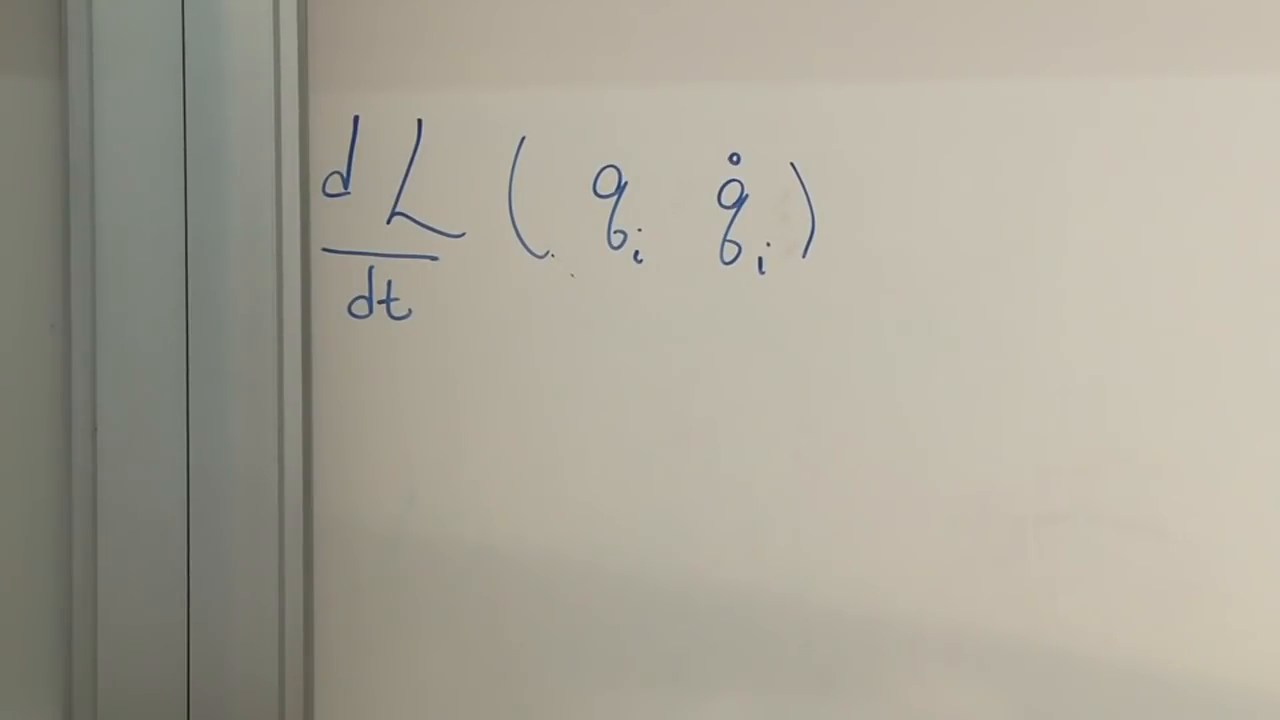
\includegraphics[width=0.72\textwidth]{lecture_05_figure_02.png}
  \caption{Début de la dérivation de \(L(q_i,\dot q_i)\) le long de la
  trajectoire.}
  \lectureframe{01:08:51}
\end{figure}

\begin{classroomqa}
  \audiencequestion{Ne manque-t-il pas une somme dans l’expression obtenue par la règle de dérivation en chaîne ?
  \lecturetimestamp{01:10:39--01:11:05}}
  \lecturerresponse{Oui. Chaque coordonnée et chaque vitesse peut modifier le
  lagrangien, donc les deux termes sont sommés sur \(i\).}
\end{classroomqa}

Utilisons la quantité de mouvement canonique et l’équation d’Euler--Lagrange,
\begin{equation}
  p_i=\frac{\partial L}{\partial\dot q_i},
  \qquad
  \dot p_i=\frac{\partial L}{\partial q_i}.
  \label{eq:l5-p-and-pdot}
\end{equation}
L’équation ~\eqref{eq:l5-chain-rule-no-time} devient
\begin{align}
  \frac{dL}{dt}
  &=\sum_i(\dot p_i\dot q_i+p_i\ddot q_i)
  \notag\\
  &=\frac{d}{dt}\sum_i p_i\dot q_i.
  \label{eq:l5-product-rule}
\end{align}
La ``magie'' n’est que la règle du produit.

\begin{figure}[htbp]
  \centering
  \includegraphics[width=0.84\textwidth]{lecture_05_figure_21.png}
  \caption{La règle de dérivation en chaîne, transformée à l’aide des équations du mouvement en la
  dérivée de \(\sum_i p_i\dot q_i\).}
  \lectureframe{01:13:45}
\end{figure}

\begin{classroomqa}
  \audiencequestion{Le dernier \(q_i\) dans le produit doit-il porter un point ou
  deux ?
  \lecturetimestamp{01:14:31--01:15:32}}
  \lecturerresponse{Dans le produit, il s’agit de \(p_i\dot q_i\), avec un seul point.
  La dérivation du produit donne
  \(\dot p_i\dot q_i+p_i\ddot q_i\), ce qui explique les deux points dans le
  deuxième terme développé.}
\end{classroomqa}

La soustraction des deux dérivées donne une combinaison conservée. Par convention
historique, on choisit son opposé et on l’appelle le hamiltonien :
\begin{equation}
  H=\sum_i p_i\dot q_i-L.
  \label{eq:l5-hamiltonian-definition}
\end{equation}

\begin{figure}[htbp]
  \centering
  \includegraphics[width=0.80\textwidth]{lecture_05_figure_22.png}
  \caption{La combinaison conservée \(L-\sum_i p_i\dot q_i=-H\) et la définition du hamiltonien.}
  \lectureframe{01:18:05}
\end{figure}

Pour une particule dans un potentiel,
\begin{equation}
  L=\frac12m\dot x^2-V(x),
  \qquad p=m\dot x.
  \label{eq:l5-particle-lagrangian}
\end{equation}
On obtient donc
\begin{align}
  H&=p\dot x-L
  \notag\\
   &=m\dot x^2-\left(\frac12m\dot x^2-V(x)\right)
  \notag\\
   &=\frac12m\dot x^2+V(x)=T+V.
  \label{eq:l5-particle-energy}
\end{align}

\begin{figure}[htbp]
  \centering
  \includegraphics[width=0.86\textwidth]{lecture_05_figure_23.png}
  \caption{Le hamiltonien d’une particule dans un potentiel se réduit à la somme familière
  de l’énergie cinétique et de l’énergie potentielle.}
  \lectureframe{01:20:50}
\end{figure}

La dérivation ne supposait aucune forme particulière pour \(L\). Ainsi,
l’équation ~\eqref{eq:l5-hamiltonian-definition}, plutôt que \(T+V\), constitue la définition générale
de l’énergie dans ce formalisme.

\section{Dépendance explicite en temps et échange d’énergie}

Rétablissons la dépendance explicite en temps dans la règle de dérivation en chaîne :
\begin{equation}
  \frac{dL}{dt}
  =\sum_i\left(
    \frac{\partial L}{\partial q_i}\dot q_i
    +\frac{\partial L}{\partial\dot q_i}\ddot q_i
  \right)
  +\frac{\partial L}{\partial t}.
  \label{eq:l5-full-chain-rule}
\end{equation}
Le membre de gauche est la dérivée totale le long du mouvement. La dérivée partielle finale
est calculée à \(q\) et \(\dot q\) fixés et porte uniquement sur les paramètres qui varient extérieurement. En répétant la même étape fondée sur la règle du produit, on obtient
\begin{equation}
  \boxed{\frac{dH}{dt}=-\frac{\partial L}{\partial t}}.
  \label{eq:l5-hamiltonian-time}
\end{equation}

\begin{figure}[htbp]
  \centering
  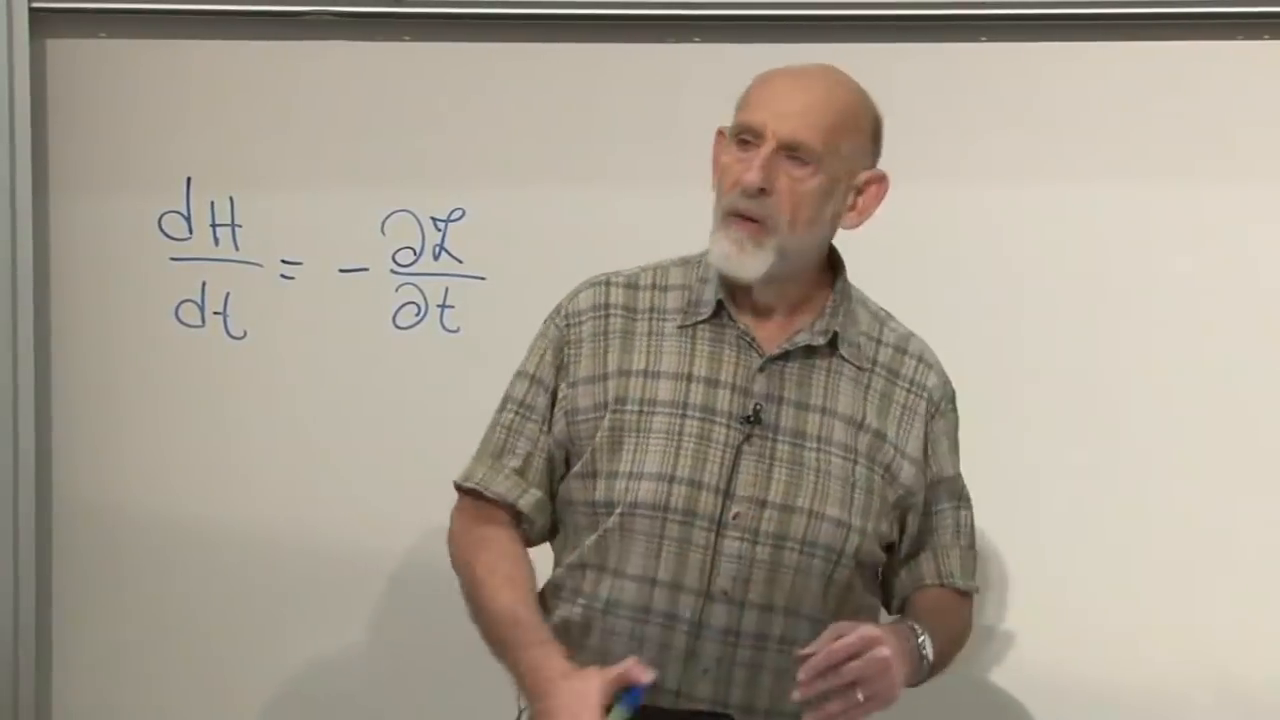
\includegraphics[width=0.70\textwidth]{lecture_05_figure_04.png}
  \caption{Le hamiltonien ne varie qu’en raison de la dépendance explicite en temps du lagrangien.}
  \lectureframe{01:37:22}
\end{figure}

Pour l’oscillateur soumis à une excitation de l’équation ~\eqref{eq:l5-driven-oscillator},
\begin{equation}
  \frac{\partial L}{\partial t}
  =-\frac12\dot k(t)x^2,
  \qquad
  \dot H=\frac12\dot k(t)x^2.
  \label{eq:l5-driven-energy-rate}
\end{equation}
En \(x=0\), le taux instantané s’annule ; en dehors de l’origine, la variation de la constante de
raideur fournit un travail à un taux proportionnel à \(x^2\dot k\).

\begin{classroomqa}
  \audiencequestion{Si l’énergie n’est pas conservée, sa définition est-elle la dérivée temporelle
  du hamiltonien ?
  \lecturetimestamp{01:27:11--01:28:04}}
  \lecturerresponse{Non. L’énergie est \(H\). Sa dérivée indique comment
  cette énergie varie. Lorsque le lagrangien prend la forme familière, \(H=T+V\) ;
  sinon, l’équation ~\eqref{eq:l5-hamiltonian-definition} en donne
  la définition. Agrandir le système pour y inclure le dispositif qui impose l’évolution rétablit
  la conservation du hamiltonien total.}
\end{classroomqa}

\begin{classroomqa}
  \audiencequestion{Qu’en est-il de l’observateur évoqué précédemment sur un
  manège en rotation, pour lequel apparaissaient les termes centrifuge et de Coriolis ?
  \lecturetimestamp{01:28:08--01:29:52}}
  \lecturerresponse{Un système de coordonnées en rotation uniforme constitue un
  changement de variables dépendant du temps, et non une symétrie spatiale fixe ni une
  simple translation dans le temps. Son lagrangien transformé peut servir à
  construire un hamiltonien, mais mieux vaut reporter ce calcul distinct
  à l’étude des forces magnétiques, car l’algèbre a une forme étroitement
  apparentée.}
\end{classroomqa}

\section{La boîte à outils lagrangienne en un coup d’œil}

On peut maintenant résumer toute la structure sous forme d’un ensemble compact de formules :
\begin{align}
  L&=L(q_i,\dot q_i,t),
  \notag\\
  p_i&=\frac{\partial L}{\partial\dot q_i},
  \qquad
  \dot p_i=\frac{\partial L}{\partial q_i},
  \notag\\
  \delta q_i&=\epsilon f_i(q)
  \quad\Longrightarrow\quad
  Q=\sum_i p_i f_i(q),\quad \dot Q=0,
  \notag\\
  H&=\sum_i p_i\dot q_i-L,
  \qquad
  \dot H=-\frac{\partial L}{\partial t}.
  \label{eq:l5-toolkit}
\end{align}

\begin{figure}[htbp]
  \centering
  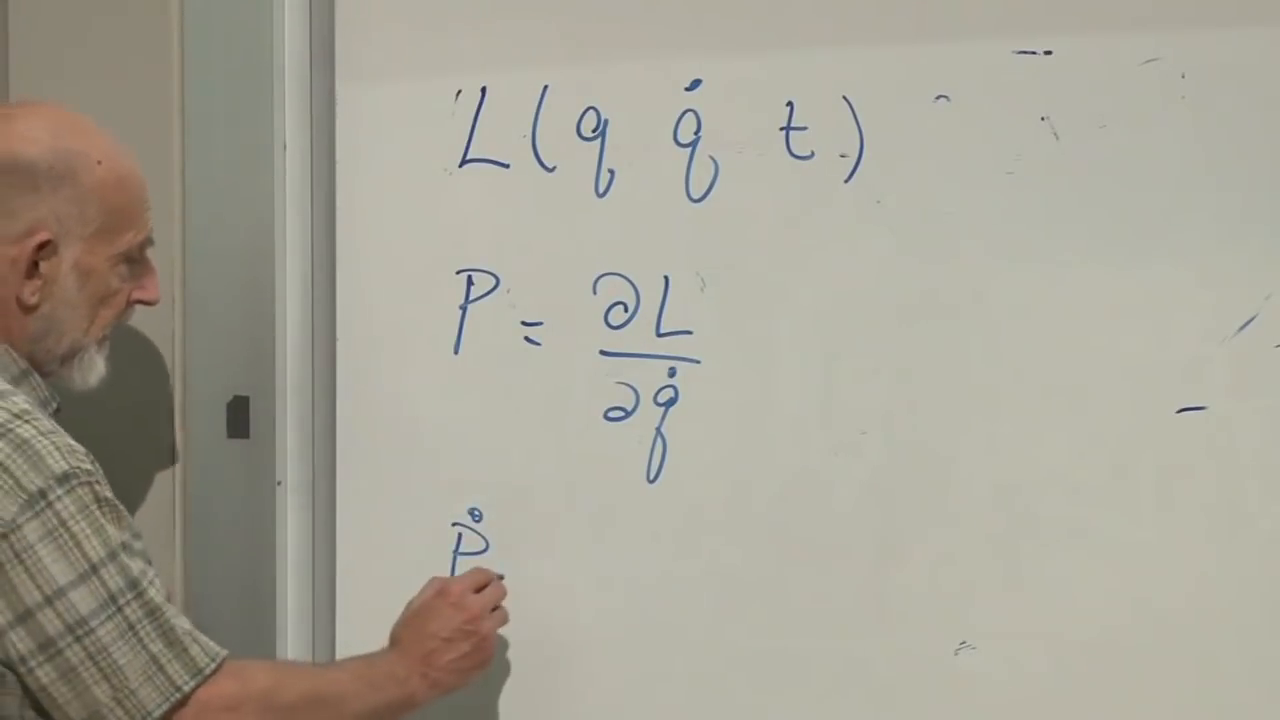
\includegraphics[width=0.66\textwidth]{lecture_05_figure_03.png}
  \caption{Le récapitulatif au tableau commence par \(L(q,\dot q,t)\), la quantité de mouvement canonique
  et l’équation d’Euler--Lagrange.}
  \lectureframe{01:31:37}
\end{figure}

Ces formules comprennent une définition, les équations du mouvement, la charge d’une
symétrie continue ordinaire et la charge associée à la translation dans le temps. Il y a
peu d’astuces ; l’essentiel est de savoir les redémontrer plutôt que de
mémoriser des expressions sans lien entre elles.

\section{Pourquoi utiliser la mécanique lagrangienne ou hamiltonienne ?}

\begin{classroomqa}
  \audiencequestion{Peut-on décrire la mécanique aussi bien avec \(L\) qu’avec \(H\),
  et pourquoi choisir l’une ou l’autre formulation ?
  \lecturetimestamp{01:37:16--01:39:18}}
  \lecturerresponse{Elles sont équivalentes lorsque la transformation de Legendre est
  régulière, mais elles mettent en avant des structures différentes. La formulation lagrangienne part
  naturellement du principe d’action stationnaire. La mécanique hamiltonienne est plus abstraite
  au début, mais ses équations sont simples et elle devient centrale en mécanique
  quantique. Le hamiltonien est l’énergie, mais son rôle dépasse largement la seule
  loi de conservation.}
\end{classroomqa}

\begin{classroomqa}
  \audiencequestion{Newton connaissait-il la forme hamiltonienne de la conservation
  de l’énergie ?
  \lecturetimestamp{01:39:29--01:39:56}}
  \lecturerresponse{Pas sous cette forme, d’après ce que l’on peut déduire des sources historiques.
  Le cadre formulé par Newton reposait sur la loi de force \(F=ma\).}
\end{classroomqa}

\begin{classroomqa}
  \audiencequestion{Pourquoi tout système physique devrait-il posséder un lagrangien ?
  Est-ce simplement un fait expérimental ?
  \lecturetimestamp{01:39:57--01:42:37}}
  \lecturerresponse{Pour les systèmes fermés considérés ici, c’est un fait empirique,
  et cela découle aussi de la description quantique plus fondamentale. On peut inventer des équations
  différentielles mathématiquement cohérentes qui ne sont pas des équations d’Euler--Lagrange. Par exemple, \(\dot x=-x\) se résout parfaitement,
  mais, en tant que loi fondamentale à une coordonnée pour un système fermé, elle présente le caractère dissipatif
  d’une perte d’information. La mécanique classique ne précède pas logiquement
  la mécanique quantique ; sa structure fondamentale lui vient de la mécanique
  quantique. Il faudra attendre pour en connaître la raison détaillée.}
\end{classroomqa}

\begin{classroomqa}
  \audiencequestion{Si tout système réel fermé possède un lagrangien, chaque
  fonction que nous appelons lagrangien correspond-elle à un système présent dans la nature ?
  \lecturetimestamp{01:42:39--01:42:54}}
  \lecturerresponse{Non. Le calcul formel admet de nombreuses fonctions qui ne
  correspondent à aucun système physique connu.}
\end{classroomqa}

\begin{classroomqa}
  \audiencequestion{Le lagrangien sert-il principalement à inventer des
  potentiels ?
  \lecturetimestamp{01:42:54--01:43:32}}
  \lecturerresponse{Son rôle est plus large. Il peut aider à organiser des systèmes
  mécaniques candidats, et c’est souvent la voie pratique la plus courte pour obtenir les
  équations du mouvement.}
\end{classroomqa}

Le double pendule illustre cet avantage pratique. Choisissons deux angles,
calculons les vitesses des deux masses en fonction de ces angles et de leurs dérivées temporelles,
formons \(T-V\), puis laissons les équations d’Euler--Lagrange traiter implicitement les
forces de contrainte. La démarche est nettement plus simple que de résoudre toutes les tensions
et accélérations à l’aide de \(F=ma\).

\begin{figure}[htbp]
  \centering
  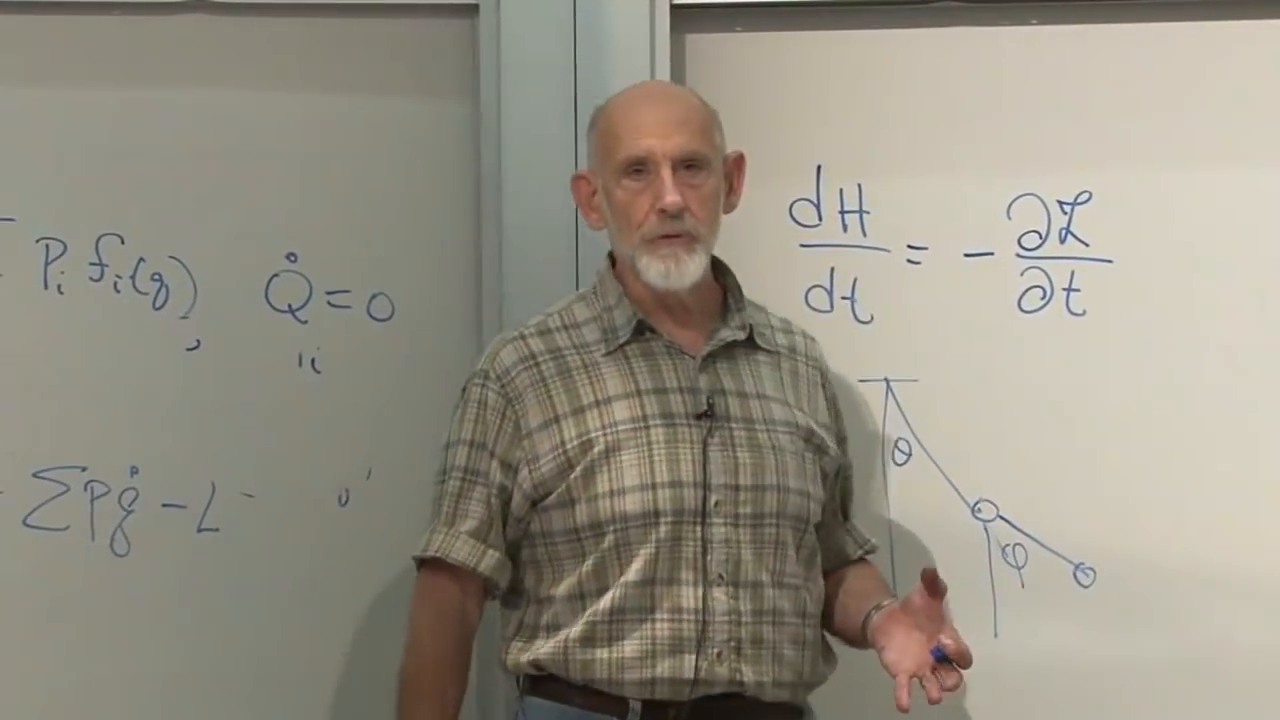
\includegraphics[width=0.84\textwidth]{lecture_05_figure_05.png}
  \caption{L’identité donnant le taux de variation de l’énergie reste au tableau à côté du
  schéma du double pendule.}
  \lectureframe{01:45:39}
\end{figure}

\begin{figure}[htbp]
  \centering
  \begin{tikzpicture}[scale=1.15]
    \draw[thick] (-0.5,0) -- (0.5,0);
    \fill (0,0) circle (0.045);
    \draw[dashed] (0,0) -- (0,-2.3);
    \draw[thick] (0,0) -- (-0.92,-1.22);
    \fill (-0.92,-1.22) circle (0.07);
    \draw[dashed] (-0.92,-1.22) -- (-0.92,-2.55);
    \draw[thick] (-0.92,-1.22) -- (-0.25,-2.18);
    \fill (-0.25,-2.18) circle (0.07);
    \draw (0,-0.55) arc (-90:-127:0.55);
    \node at (-0.42,-0.56) {$\theta$};
    \draw (-0.92,-1.72) arc (-90:-55:0.48);
    \node at (-0.56,-1.72) {$\phi$};
  \end{tikzpicture}
  \caption{Coordonnées angulaires généralisées d’un double pendule.}
\end{figure}

Le changement de variables est tout aussi efficace : on transforme un lagrangien puis
on en déduit les équations, au lieu de transformer séparément chaque équation des forces.

\begin{classroomqa}
  \audiencequestion{Le pendule double est-il essentiellement un autre système à trois corps, comme le Soleil, la Terre et la Lune, où l’un des corps jouerait le rôle d’ancrage ?
  \lecturetimestamp{01:45:06--01:45:25}}
  \lecturerresponse{Cette analogie rend bien compte de la hiérarchie, même si les tiges imposent des contraintes différentes. Dans les deux cas, on peut, dans une approximation, traiter un composant très massif ou fixe comme structure de référence.}
\end{classroomqa}

\begin{classroomqa}
  \audiencequestion{Le pendule double utilise \(T-V\), alors que nous venons d’insister sur le fait que les lagrangiens peuvent être plus généraux. Dans quels cas \(T-V\) est-il valable ?
  \lecturetimestamp{01:46:08--01:46:58}}
  \lecturerresponse{Cette forme usuelle s’applique aux particules non relativistes ordinaires décrites dans un référentiel inertiel, en l’absence de couplage magnétique dépendant de la vitesse. Les référentiels en rotation, les systèmes relativistes et les champs magnétiques nécessitent des termes plus généraux.}
\end{classroomqa}

\begin{classroomqa}
  \audiencequestion{Les collisions échappent-elles à cette description ?
  \lecturetimestamp{01:47:00--01:48:05}}
  \lecturerresponse{Les collisions élastiques résultent de forces de courte portée et donc de potentiels. À l’échelle microscopique, les collisions inélastiques restent mécaniques, mais de l’énergie est transférée aux vibrations internes, à la déformation et à la chaleur. Une description du centre de masse qui omet ces degrés de liberté est incomplète.}
\end{classroomqa}

\begin{classroomqa}
  \audiencequestion{Peut-on analyser une balle de baseball frappée par une batte à l’aide de \(F=ma\) ?
  \lecturetimestamp{01:48:05--01:48:33}}
  \lecturerresponse{Seulement à un niveau approximatif. Une description complète doit prendre en compte la déformation, l’échauffement, les dommages éventuels à la balle et peut-être même la rupture de la batte. Ces degrés de liberté internes expliquent pourquoi un impact réaliste est bien plus difficile à décrire qu’une collision entre particules ponctuelles.}
\end{classroomqa}

\begin{classroomqa}
  \audiencequestion{Qu’en est-il d’un solide étendu ?
  \lecturetimestamp{01:48:34--01:49:00}}
  \lecturerresponse{On peut étudier les solides soit par les méthodes newtoniennes, soit à l’aide d’un lagrangien \(T-V\) écrit en coordonnées de translation et de rotation. Construire ce lagrangien est un exercice utile.}
\end{classroomqa}

\begin{classroomqa}
  \audiencequestion{La relation d’incertitude quantique entre l’énergie et le --temps signifie-t-elle que l’énergie n’est pas strictement conservée ?
  \lecturetimestamp{01:49:01--01:49:29}}
  \lecturerresponse{Non. L’énergie peut être strictement conservée. Cette relation signifie que déterminer l’énergie avec une grande précision exige une observation de longue durée ; elle ne remplace pas la loi de conservation.}
\end{classroomqa}

\begin{classroomqa}
  \audiencequestion{La mécanique newtonienne et la mécanique lagrangienne sont-elles logiquement équivalentes ?
  \lecturetimestamp{01:49:36--01:50:07}}
  \lecturerresponse{Elles sont équivalentes dans le domaine usuel où les deux formulations s’appliquent. On peut néanmoins inventer des lagrangiens dont les équations ne ressemblent pas à la forme élémentaire \(m\ddot x=F(x)\).}
\end{classroomqa}

\section{Un terme cinétique dépendant des coordonnées}

Considérons l’exemple volontairement peu familier
\begin{equation}
  L=\frac12q^2\dot q^2-\frac12q^2.
  \label{eq:l5-nonstandard-l}
\end{equation}
Il s’agit d’un lagrangien valide dont le coefficient cinétique dépend des coordonnées. On pourrait également considérer des termes linéaires en vitesse, tels que \(q\dot q\) ; dans cet exemple à une dimension, ce terme particulier est une dérivée totale et ne modifierait pas les équations du mouvement.

La quantité de mouvement canonique est
\begin{equation}
  p=\frac{\partial L}{\partial\dot q}=q^2\dot q,
  \label{eq:l5-nonstandard-p}
\end{equation}
donc
\begin{equation}
  \dot p=q^2\ddot q+2q\dot q^2,
  \qquad
  \frac{\partial L}{\partial q}=q\dot q^2-q.
  \label{eq:l5-nonstandard-derivatives}
\end{equation}
L’équation du mouvement est donc
\begin{equation}
  q^2\ddot q+q\dot q^2=-q.
  \label{eq:l5-nonstandard-eom}
\end{equation}

\begin{figure}[htbp]
  \centering
  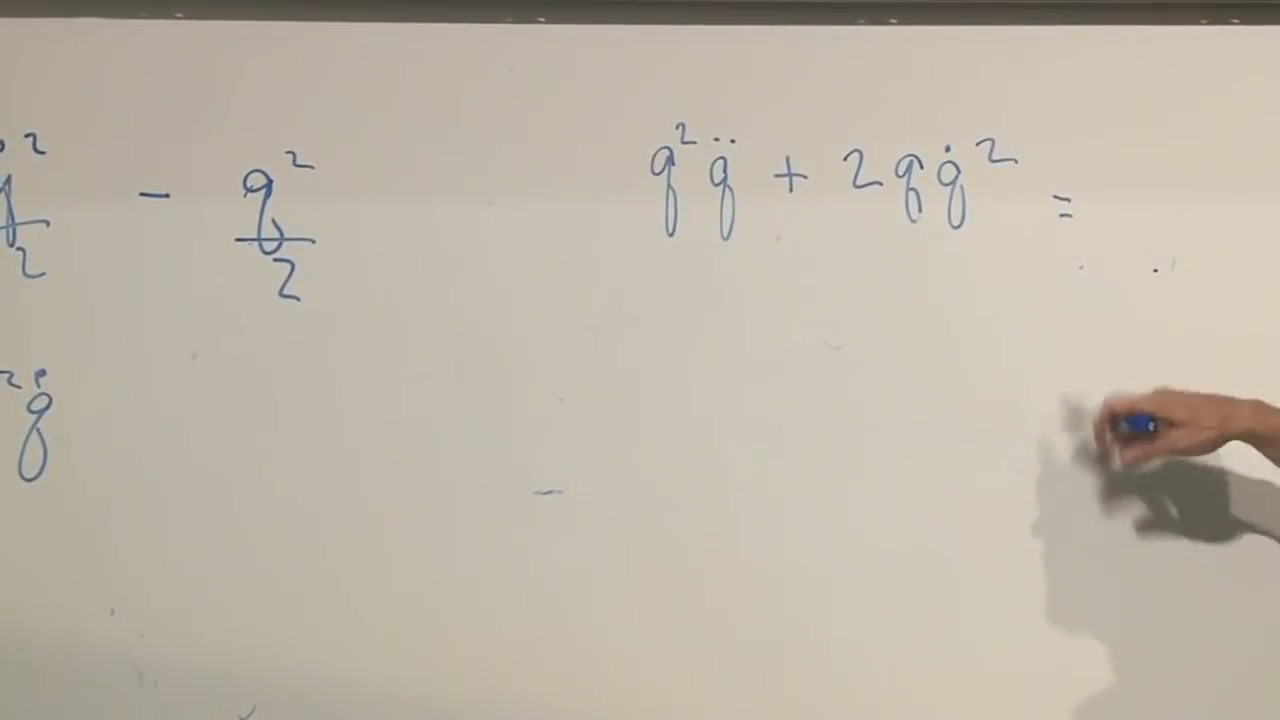
\includegraphics[width=0.80\textwidth]{lecture_05_figure_06.png}
  \caption{La quantité de mouvement dérivée dans l’exemple où le terme cinétique dépend des coordonnées.}
  \lectureframe{01:52:32}
\end{figure}

\begin{classroomqa}
  \audiencequestion{Peut-on diviser l’équation par \(q\) ?
  \lecturetimestamp{01:53:22--01:53:39}}
  \lecturerresponse{Seulement lorsque \(q\neq0\). Pour \(q=0\), le coefficient cinétique et l’application de Legendre sont dégénérés ; une division ferait donc disparaître un point singulier qui doit être traité séparément.}
\end{classroomqa}

Le hamiltonien est
\begin{align}
  H&=p\dot q-L
  \notag\\
   &=q^2\dot q^2-
     \left(\frac12q^2\dot q^2-\frac12q^2\right)
  \notag\\
   &=\frac12q^2\dot q^2+\frac12q^2.
  \label{eq:l5-nonstandard-h}
\end{align}

\begin{classroomqa}
  \audiencequestion{Peut-on encore appeler \(q^2\dot q^2/2\) l’énergie cinétique ?
  \lecturetimestamp{01:54:41--01:55:07}}
  \lecturerresponse{Oui. Dans cet exemple développé, le hamiltonien a de nouveau l’apparence d’un terme cinétique positif auquel s’ajoute un terme de potentiel. L’essentiel est que les définitions formelles ont fonctionné sans qu’il soit nécessaire de supposer au préalable la forme élémentaire à masse constante.}
\end{classroomqa}

\section{Dissipation et origine profonde du formalisme}

\begin{classroomqa}
  \audiencequestion{Comment inclure le frottement dans un lagrangien ?
  \lecturetimestamp{01:55:09--01:56:17}}
  \lecturerresponse{Pas comme force fondamentale dans le système fermé simple à nombre fini de degrés de liberté considéré ici. Le frottement macroscopique est un effet statistique dû à un très grand nombre de degrés de liberté microscopiques. Ces atomes obéissent toujours à la mécanique sous-jacente, mais une description réduite qui ne les suit pas fait apparaître une dissipation.}
\end{classroomqa}

\begin{classroomqa}
  \audiencequestion{Comment Hamilton est-il parvenu à sa formulation ?
  \lecturetimestamp{01:56:22--01:56:37}}
  \lecturerresponse{Aucune dérivation historique n’a été présentée ici. Pour le cours actuel, l’essentiel est de comprendre le fonctionnement de cette formulation.}
\end{classroomqa}

\begin{classroomqa}
  \audiencequestion{Existe-t-il une méthode plus générale pour obtenir un lagrangien lorsqu’il n’a pas manifestement la forme \(T-V\) ?
  \lecturetimestamp{01:56:43--01:58:54}}
  \lecturerresponse{L’expérience, une conjecture éclairée, un principe de symétrie ou la reconstruction à partir des équations souhaitées peuvent fournir la fonction. Demander au calcul lui-même d’où vient son entrée revient à demander à la définition d’une dérivée d’où vient \(f(x)\). Le calcul nous indique quoi faire une fois la fonction spécifiée. La mécanique quantique apporte, à un niveau plus profond, une réponse à la question de savoir pourquoi les systèmes fermés de la nature obéissent à cette structure abstraite.}
\end{classroomqa}

Ce point rejoint les thèmes abordés au début du cours. L’évolution hamiltonienne fondamentale est déterministe et réversible, en ce sens que les trajectoires ne fusionnent pas et que l’information n’est pas simplement détruite. Le lien entre cette propriété et la formulation dans l’espace des phases sera développé progressivement.

\begin{classroomqa}
  \audiencequestion{Le calcul variationnel s’est-il contenté de remonter à partir des équations classiques souhaitées, et la mécanique quantique obtient-elle son lagrangien de la même manière ?
  \lecturetimestamp{01:59:37--02:01:07}}
  \lecturerresponse{Dans la construction classique élémentaire, on peut effectivement choisir une action dont les trajectoires stationnaires reproduisent les équations connues. En mécanique quantique, l’ordre logique est différent : on part naturellement du hamiltonien pour aboutir à une description lagrangienne. Le hamiltonien y est plus intuitif, même s’il paraît d’abord abstrait en mécanique classique.}
\end{classroomqa}

\begin{classroomqa}
  \audiencequestion{La mécanique quantique peut-elle décrire le frottement ?
  \lecturetimestamp{02:01:08--02:02:05}}
  \lecturerresponse{Oui, mais une description fondamentale doit inclure les degrés de liberté de l’environnement. On ne peut décrire complètement une particule se déplaçant dans un fluide visqueux sans inclure les particules du fluide. Le frottement est l’effet collectif complexe qui émerge lorsque ces degrés de liberté ne sont pas suivis individuellement.}
\end{classroomqa}

\chapter{Systèmes contraints et dynamique hamiltonienne}

\lectureoverview{Deux systèmes contraints montrent pourquoi la mécanique lagrangienne est si efficace : une fois les coordonnées appropriées choisies, les équations du mouvement et leurs lois de conservation s’obtiennent sans calcul explicite des forces de contrainte. Ces mêmes exemples conduisent ensuite à la mécanique hamiltonienne, où les coordonnées et les moments forment l’espace des phases, où l’oscillateur harmonique devient une rotation rigide et où les deux équations du premier ordre de Hamilton remplacent chaque équation d’Euler--Lagrange.}

\section{Ce que signifie résoudre un problème de mécanique}

Le but immédiat de la méthode lagrangienne est pratique. Un coin qui glisse sur un sol et un double pendule peuvent tous deux être traités avec les lois de Newton, mais les inconnues que sont les forces de contact et les tensions rendent vite les calculs pénibles. Une fois les règles de la mécanique lagrangienne connues, ces mêmes problèmes se ramènent à une suite d’étapes maîtrisées :
\begin{enumerate}
  \item choisir des coordonnées indépendantes qui décrivent une configuration instantanée ;
  \item exprimer l’énergie cinétique et l’énergie potentielle en fonction de ces coordonnées ;
  \item former \(L=T-V\) et appliquer les équations d’Euler--Lagrange.
\end{enumerate}

Pour l’objectif présent, un problème est déjà \emph{résolu} dès lors que ses équations du mouvement ont été correctement écrites. On peut encore chercher une trajectoire sous forme fermée, mais c’est une question distincte. Les équations différentielles non linéaires peuvent être intégrées numériquement une fois le système mécanique établi. La difficulté ne réside souvent pas dans l’intégration, mais dans le choix de variables qui incorporent les contraintes sans introduire de forces inconnues redondantes.

\section{Une particule qui glisse sur un coin mobile}

Considérons un coin de masse \(M\) astreint à glisser sans frottement sur un plan horizontal. Une particule ponctuelle de masse \(m\) est astreinte à rester sur la face inclinée. Le système possède deux degrés de liberté : l’un indique la position du coin, l’autre la position de la particule sur le coin.

Posons
\begin{equation}
  \begin{aligned}
    X&=\text{horizontal position of the wedge corner},\\
    x&=\text{horizontal displacement of the particle}\\[-0.2em]
     &\phantom{={}}\text{from that corner}.
  \end{aligned}
  \label{eq:l6-wedge-coordinates}
\end{equation}
La coordonnée horizontale absolue de la particule est donc \(X+x\). Ce choix n’est pas unique. On pourrait aussi utiliser la distance parcourue le long de la pente ou la coordonnée horizontale absolue de la particule. Toute paire non redondante qui décrit les mêmes configurations est légitime, même si certaines paires mettent mieux en évidence la structure que d’autres.

Pour un angle de pente fixe \(\beta\), le déplacement vertical \(y\) n’est pas une coordonnée indépendante :
\begin{equation}
  y=x\tan\beta,
  \qquad
  \dot y=\dot x\tan\beta.
  \label{eq:l6-wedge-constraint}
\end{equation}
Nous nous plaçons dans le cas \(\beta=45^\circ\), de sorte que \(y=x\) et
\(\dot y=\dot x\). Cette simplification élimine les facteurs trigonométriques sans rien changer à l’objet de l’exemple.

\begin{figure}[htbp]
  \centering
  \includegraphics[width=0.84\textwidth]{lecture_06_figure_06.png}
  \caption{Le coin mobile, la particule contrainte et les composantes horizontale et verticale de la vitesse utilisées dans l’exemple à \(45^\circ\).}
  \lectureframe{00:10:25}
\end{figure}

L’énergie cinétique du coin est
\begin{equation}
  T_{M}=\frac{M}{2}\dot X^2.
  \label{eq:l6-wedge-kinetic}
\end{equation}
La vitesse horizontale de la particule est \(\dot X+\dot x\), tandis que sa vitesse verticale est \(\dot x\). Son énergie cinétique est donc
\begin{equation}
  T_m=\frac{m}{2}\left[(\dot X+\dot x)^2+\dot x^2\right].
  \label{eq:l6-particle-kinetic}
\end{equation}
En choisissant \(x=0\) comme niveau de référence de l’énergie potentielle gravitationnelle, on a \(V=mgx\).
Ainsi,
\begin{equation}
  L=\frac{M}{2}\dot X^2
    +\frac{m}{2}\left[(\dot X+\dot x)^2+\dot x^2\right]
    -mgx.
  \label{eq:l6-wedge-lagrangian}
\end{equation}

\begin{figure}[htbp]
  \centering
  \includegraphics[width=0.86\textwidth]{lecture_06_figure_07.png}
  \caption{La géométrie du coin, \(V=mgx\), et les deux contributions à l’énergie cinétique réunies au tableau.}
  \lectureframe{00:14:15}
\end{figure}

\subsection{Le moment canonique est défini par le lagrangien}

Les moments canoniques sont définis par le lagrangien, et non devinés à partir de la vitesse d’une particule prise isolément :
\begin{align}
  p_X&=\frac{\partial L}{\partial\dot X}
      =M\dot X+m(\dot X+\dot x),
      \label{eq:l6-wedge-pX}\\
  p_x&=\frac{\partial L}{\partial\dot x}
      =m(\dot X+\dot x)+m\dot x.
      \label{eq:l6-wedge-px}
\end{align}
La première expression est la quantité de mouvement horizontale totale ordinaire : le coin contribue à hauteur de \(M\dot X\), et la particule à hauteur de \(m(\dot X+\dot x)\). Elle apparaît ici comme le moment conjugué à la coordonnée \(X\).

\begin{figure}[htbp]
  \centering
  \includegraphics[width=0.86\textwidth]{lecture_06_figure_08.png}
  \caption{Les moments canoniques conjugués à la coordonnée du coin \(X\) et à la coordonnée relative de la particule \(x\).}
  \lectureframe{00:18:05}
\end{figure}

Le lagrangien ne dépend pas explicitement de \(X\). Une translation horizontale de l’ensemble du dispositif agit ainsi :
\begin{equation}
  \delta X=\epsilon,
  \qquad
  \delta x=0.
  \label{eq:l6-wedge-translation}
\end{equation}
La règle générale des symétries infinitésimales
\begin{equation}
  \delta q_i=\epsilon f_i(q),
  \qquad
  Q=\sum_i p_i f_i
  \label{eq:l6-noether-rule}
\end{equation}
donne donc \(Q=p_X\). De façon équivalente, \(X\) est une coordonnée cyclique et
\begin{equation}
  \dot p_X=\frac{\partial L}{\partial X}=0.
  \label{eq:l6-wedge-conservation}
\end{equation}

Il n’existe pas de symétrie correspondante par translation verticale. Le coin ne peut pas se déplacer verticalement, et une variation de la hauteur de la particule modifie l’énergie potentielle gravitationnelle. La quantité de mouvement horizontale se conserve ; la quantité de mouvement verticale de ce sous-système contraint, elle, ne se conserve pas.

Pour la coordonnée relative, l’équation d’Euler--Lagrange est
\begin{equation}
  \dot p_x=\frac{\partial L}{\partial x}=-mg.
  \label{eq:l6-wedge-force}
\end{equation}
Un signe a dû être corrigé au tableau à cette étape. La méthode fiable consiste à partir de \(L=T-V\) : puisque \(V=mgx\), la dérivée du lagrangien vaut \(-mg\). Le fait que \(x\) ait été introduit comme un déplacement horizontal ne supprime pas la gravité de son équation, car la contrainte relie ce déplacement horizontal à la hauteur verticale \(y=x\).

Aucune force normale ni force de réaction n’est apparue. Ces forces prennent les valeurs nécessaires au maintien des contraintes. La méthode de Newton les introduirait et les déterminerait en même temps que les accélérations ; les coordonnées généralisées les rendent inutiles.

\section{Le double pendule et l’art de choisir les coordonnées}

Suspendons maintenant deux masses unitaires à deux tiges sans masse de longueur unitaire. La première tige fait un angle \(\theta\) avec la verticale descendante. Pour le second degré de liberté, nous avons le choix. Nous pouvons utiliser un deuxième angle absolu \(\phi\) ou l’angle relatif \(\alpha\) entre les tiges.

L’angle relatif est le choix le plus révélateur. Supprimons provisoirement la gravité. Une rotation rigide de l’ensemble du dispositif modifie son orientation absolue, mais pas l’angle entre les tiges :
\begin{equation}
  \theta\longrightarrow\theta+\epsilon,
  \qquad
  \alpha\longrightarrow\alpha.
  \label{eq:l6-double-rotation}
\end{equation}
Avec ce choix, la symétrie de rotation agit sur une seule coordonnée. Cela ne rend pas incorrects les autres systèmes de coordonnées. Cela rend la symétrie, et donc la quantité conservée, plus facile à repérer.

\begin{figure}[htbp]
  \centering
  \includegraphics[width=0.76\textwidth]{lecture_06_figure_09.png}
  \caption{Le double pendule, avec \(\theta\) comme premier angle absolu et \(\alpha\) comme angle de la seconde tige par rapport à la première.}
  \lectureframe{00:29:20}
\end{figure}

Pour obtenir l’énergie cinétique, utilisons provisoirement les coordonnées cartésiennes comme auxiliaires de calcul. La coordonnée verticale étant mesurée vers le bas, le premier pendule se trouve en
\begin{equation}
  x_1=\sin\theta,
  \qquad
  y_1=\cos\theta,
  \label{eq:l6-bob-one-position}
\end{equation}
et donc
\begin{equation}
  \dot x_1=\dot\theta\cos\theta,
  \qquad
  \dot y_1=-\dot\theta\sin\theta,
  \qquad
  \dot x_1^2+\dot y_1^2=\dot\theta^2.
  \label{eq:l6-bob-one-velocity}
\end{equation}
Le second pendule se trouve en
\begin{align}
  x_2&=\sin\theta+\sin(\theta+\alpha),\\
  y_2&=\cos\theta+\cos(\theta+\alpha),
  \label{eq:l6-bob-two-position}
\end{align}
d’où, par exemple,
\begin{equation}
  \dot x_2=\dot\theta\cos\theta
  +(\dot\theta+\dot\alpha)\cos(\theta+\alpha),
  \label{eq:l6-bob-two-xvelocity}
\end{equation}
et une expression analogue pour \(\dot y_2\).

\begin{figure}[htbp]
  \centering
  \includegraphics[width=0.88\textwidth]{lecture_06_figure_10.png}
  \caption{Coordonnées cartésiennes auxiliaires des deux pendules. Elles servent à calculer les vitesses et ne sont pas introduites comme degrés de liberté supplémentaires.}
  \lectureframe{00:35:25}
\end{figure}

La somme des deux énergies cinétiques donne le résultat cohérent ci-dessous. Le terme croisé découle de
\begin{equation*}
  \cos A\cos B+\sin A\sin B=\cos(A-B).
\end{equation*}
\begin{equation}
  T=\dot\theta^2
    +\frac12(\dot\theta+\dot\alpha)^2
    +\dot\theta(\dot\theta+\dot\alpha)\cos\alpha.
  \label{eq:l6-double-kinetic}
\end{equation}

\begin{classroomqa}
  \audiencequestion{Cette expression comprend-elle déjà l’énergie cinétique des deux pendules, ou a-t-on perdu un facteur un demi ?
  \lecturetimestamp{00:38:06--00:38:27}}
  \lecturerresponse{Elle comprend les deux contributions. Elle provient de
  \(\tfrac12(\dot x_1^2+\dot y_1^2+\dot x_2^2+\dot y_2^2)\).
  Les deux contributions égales se combinent pour donner le premier terme
  \(\dot\theta^2\) ; aucun facteur ne manque.}
\end{classroomqa}

En l’absence de gravité, \(L=T\) ne dépend pas explicitement de \(\theta\). Ainsi,
\begin{equation}
  \dot p_\theta=\frac{\partial L}{\partial\theta}=0,
  \label{eq:l6-double-angular-conservation}
\end{equation}
et \(p_\theta\) est le moment cinétique total. Précisons le sens de l’affirmation selon laquelle \(\theta\) n’apparaît pas : \(\dot\theta\) apparaît bien, mais pas la coordonnée non dérivée.

Le rétablissement de la gravité brise la symétrie de rotation globale. Avec la convention où la verticale est orientée vers le bas, le choix commode suivant du niveau de référence donne
\begin{equation}
  V=-g(y_1+y_2)
   =-g\left[2\cos\theta+\cos(\theta+\alpha)\right].
  \label{eq:l6-double-potential}
\end{equation}
Une constante additive ne changerait rien. L’essentiel est que \(\theta\) apparaît maintenant explicitement, si bien que son moment conjugué n’est plus conservé. L’énergie, elle, reste conservée, car le lagrangien ne dépend pas explicitement du temps.

\begin{classroomqa}
  \audiencequestion{L’expression au tableau devrait-elle être
  \(\dot\theta-\dot\alpha\) plutôt que
  \(\dot\theta+\dot\alpha\) ?
  \lecturetimestamp{00:43:00--00:43:54}}
  \lecturerresponse{L’orientation adoptée ici impose le signe plus. C’est la convention de l’équation ~\eqref{eq:l6-bob-two-position}, également utilisée dans l’expression de l’énergie cinétique de l’équation ~\eqref{eq:l6-double-kinetic}. Inverser la définition du sens positif de \(\alpha\) modifierait les signes correspondants, mais il faudrait alors le faire de façon cohérente partout. Au tableau, les deux conventions ont été mélangées.}
\end{classroomqa}

\begin{figure}[htbp]
  \centering
  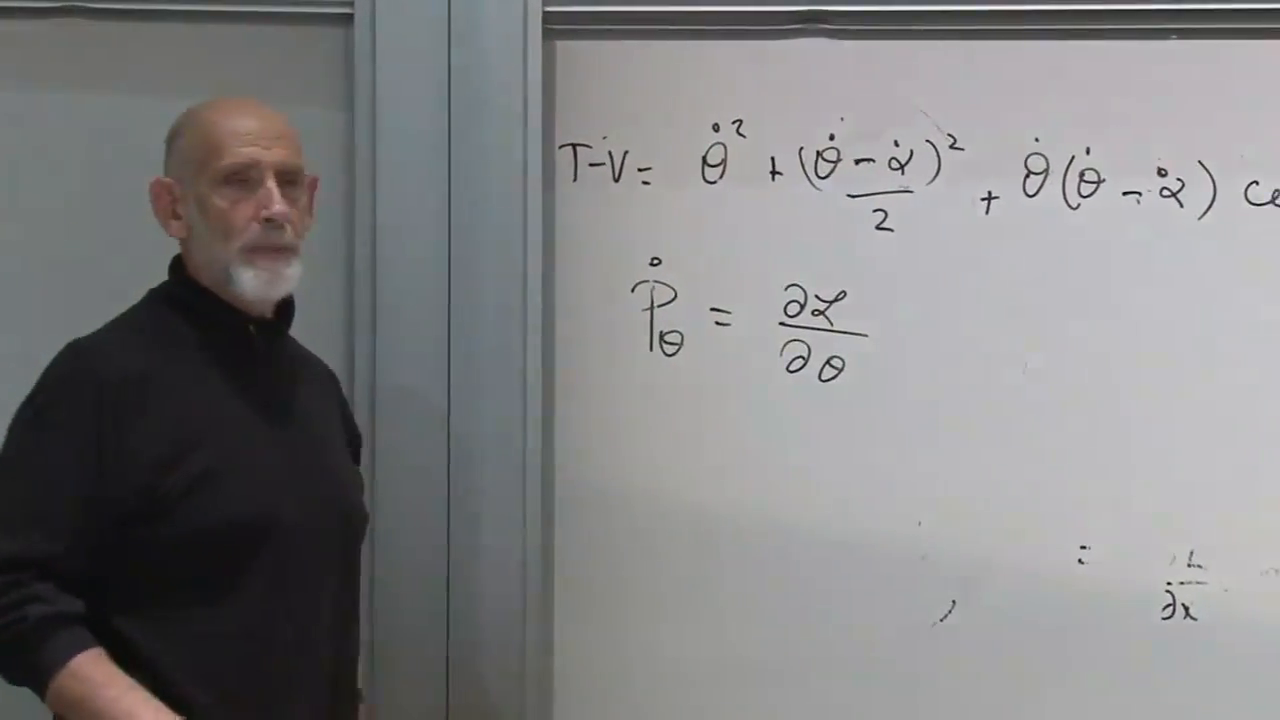
\includegraphics[width=0.84\textwidth]{lecture_06_figure_02.png}
  \caption{Le calcul du pendule sans gravité et \(\dot p_\theta=\partial L/\partial\theta\). La ligne supérieure du tableau conserve la notation locale dont les signes sont incohérents, évoquée dans la question ; la formule normalisée est donnée par l’équation ~\eqref{eq:l6-double-kinetic}.}
  \lectureframe{00:45:50}
\end{figure}

Une fois \(T\) et \(V\) connus, il ne reste qu’à obtenir les équations par dérivation. Les tensions des tiges et les forces qui imposent leur longueur fixe ont, là encore, disparu grâce au choix des coordonnées.

\subsection{Ce que la conservation implique ou n’implique pas}

\begin{classroomqa}
  \audiencequestion{Peut-on déterminer directement à partir des équations si le double pendule est chaotique ?
  \lecturetimestamp{00:44:57--00:45:25}}
  \lecturerresponse{En général, pas par une simple inspection. Quand les paramètres ou les énergies varient, un système peut passer d’un comportement régulier à un comportement chaotique. Ce sujet exige davantage que l’examen brut des équations et sera abordé plus loin.}
\end{classroomqa}

\begin{classroomqa}
  \audiencequestion{Dans un système conservatif, est-ce que chaque \(\dot p_i\) est nul ?
  \lecturetimestamp{00:45:25--00:46:24}}
  \lecturerresponse{Non. L’équation générale est
  \(\dot p_i=\partial L/\partial q_i\). Cette dérivée ne s’annule que si \(q_i\) est cyclique. Une coordonnée cyclique est le cas particulièrement simple où la symétrie se traduit par le déplacement d’une coordonnée tandis que les autres restent fixes.}
\end{classroomqa}

Si le seul objectif est de calculer l’évolution numérique, un système de coordonnées peu commode reste utilisable ; il produit simplement des équations plus longues. L’intérêt d’un choix judicieux est conceptuel : le moment conservé se voit avant même de résoudre les équations.

\begin{classroomqa}
  \audiencequestion{Sans gravité, un double pendule se comporte-t-il aussi simplement qu’un pendule libre unique ?
  \lecturetimestamp{00:47:02--00:47:35}}
  \lecturerresponse{Un rotor libre unique tourne uniformément, car son unique moment cinétique détermine son mouvement. Un double pendule peut présenter un mouvement relatif très complexe tout en conservant son moment cinétique total. Si les deux vitesses angulaires sont initialement nulles, le système reste au repos ; sinon, ses deux parties interagissent.}
\end{classroomqa}

\begin{classroomqa}
  \audiencequestion{En l’absence de gravité, \(\dot\theta\) et \(\dot\alpha\) sont-ils constants séparément ?
  \lecturetimestamp{00:47:36--00:52:42}}
  \lecturerresponse{Non. La conservation signifie \(\dot p_\theta=0\), et non \(\ddot\theta=0\) ou \(\ddot\alpha=0\). L’expression de \(p_\theta=\partial L/\partial\dot\theta\) dépend des deux vitesses angulaires et de \(\alpha\). Les tiges transmettent des couples, ce qui permet aux deux pendules d’échanger moment cinétique et énergie. C’est analogue à deux masses reliées par un ressort : la quantité de mouvement totale et la vitesse du centre de masse sont constantes, tandis que les vitesses individuelles oscillent. L’analogue rotationnel est une combinaison collective particulière, et non l’un ou l’autre angle pris séparément.}
\end{classroomqa}

\begin{classroomqa}
  \audiencequestion{Les forces qui échangent le moment cinétique sont-elles transmises par les tiges ?
  \lecturetimestamp{00:52:43--00:53:34}}
  \lecturerresponse{Oui. Une force transmise le long d’une tige n’est pas nécessairement dirigée vers le pivot de l’autre mouvement et peut donc exercer un couple. Un couple est simplement la tendance d’une force à produire une rotation ; ici, il entraîne des accélérations angulaires individuelles non nulles.}
\end{classroomqa}

\section{L’hamiltonien, troisième formulation}

L’hamiltonien est l’énergie, mais ce n’est là que sa première signification. Il est aussi au fondement d’une troisième formulation de la mécanique. Les équations de Newton utilisent les forces et les accélérations. Le principe de l’action stationnaire donne les équations d’Euler--Lagrange. Pour les systèmes réguliers, la mécanique hamiltonienne est équivalente à cette formulation, mais ses variables et sa géométrie sont différentes.

Au lieu de \(q_i\) et de \(\dot q_i\), utilisons \(q_i\) et leurs moments conjugués \(p_i\). Décrire l’état d’un système à \(n\) degrés de liberté exige \(2n\) nombres dans l’une ou l’autre formulation : positions et vitesses, ou positions et moments. Le lien entre ces descriptions est
\begin{equation}
  p_i=\frac{\partial L}{\partial\dot q_i}.
  \label{eq:l6-legendre-map}
\end{equation}
Lorsque ces relations peuvent être inversées pour exprimer les vitesses \(\dot q_i(q,p)\), on définit
\begin{equation}
  H(q,p)=\sum_i p_i\dot q_i-L(q,\dot q).
  \label{eq:l6-hamiltonian-definition}
\end{equation}
Les vitesses du membre de droite sont alors éliminées au profit de \(q\) et de \(p\). Cette inversibilité est l’hypothèse de régularité de la transformation de Legendre. Les lagrangiens singuliers exigent la théorie plus générale des contraintes ; cette construction élémentaire ne les traite pas.

\subsection{La réversibilité avant le calcul infinitésimal}

Considérons un ensemble fini d’états abstraits reliés par des flèches. Même une règle déterministe peut ne pas être réversible si deux états antérieurs aboutissent à un même état ultérieur. L’avenir est unique, mais le passé ne l’est pas. Inverser toutes les flèches produit le défaut opposé : un état se ramifie en plusieurs futurs. Dans le premier schéma, les flèches convergent ; dans le second, elles divergent.

\begin{figure}[htbp]
  \centering
  \includegraphics[width=0.86\textwidth]{lecture_06_figure_11.png}
  \caption{Applications d’états abstraits illustrant la différence entre des cycles réversibles et une convergence ou une divergence interdites.}
  \lectureframe{00:56:20}
\end{figure}

L’évolution hamiltonienne fournira la version continue de cet énoncé. Un nuage de points de l’espace des phases peut se déplacer et se déformer, mais il ne peut pas acquérir de puits qui efface les distinctions entre états, ni de source qui engendre plusieurs futurs à partir d’un seul état. La démonstration viendra plus tard ; pour l’instant, ces schémas motivent la géométrie.

\begin{classroomqa}
  \audiencequestion{Le schéma abstrait des états représente-t-il un objet qui se déplace dans un champ gravitationnel ?
  \lecturetimestamp{00:58:02--00:58:35}}
  \lecturerresponse{Non. Les points sont de simples états abstraits et les flèches définissent une règle de changement d’état. Aucune signification spatiale ou gravitationnelle n’a été attribuée au dessin.}
\end{classroomqa}

\begin{classroomqa}
  \audiencequestion{Comment distinguer une application d’états à convergence interdite d’un trou noir ?
  \lecturetimestamp{00:58:40--00:59:28}}
  \lecturerresponse{Ce n’est pas facile et la question est subtile. Elle est légitime, mais une réponse correcte exige de décrire soigneusement l’état complet et son évolution quantique et gravitationnelle. Le schéma élémentaire ne suffit pas à trancher.}
\end{classroomqa}

\section{Un oscillateur adapté à l’espace des phases}

Avant de dériver les équations générales, considérons un oscillateur harmonique écrit dans des variables délibérément adaptées :
\begin{equation}
  L=\frac{1}{2\omega}\dot q^2-\frac{\omega}{2}q^2.
  \label{eq:l6-rescaled-lagrangian}
\end{equation}
Son moment conjugué est
\begin{equation}
  p=\frac{\partial L}{\partial\dot q}=\frac{\dot q}{\omega},
  \qquad
  \dot q=\omega p.
  \label{eq:l6-rescaled-momentum}
\end{equation}
En substituant dans l’équation ~\eqref{eq:l6-hamiltonian-definition}, on obtient
\begin{align}
  H&=p\dot q-L\\
   &=\omega p^2-\frac{\omega p^2}{2}+\frac{\omega q^2}{2}
    =\frac{\omega}{2}(p^2+q^2).
  \label{eq:l6-oscillator-hamiltonian}
\end{align}

\begin{figure}[htbp]
  \centering
  \includegraphics[width=0.86\textwidth]{lecture_06_figure_12.png}
  \caption{Transformation de Legendre de l’oscillateur adapté et hamiltonien symétrique \(H=\tfrac{\omega}{2}(p^2+q^2)\).}
  \lectureframe{01:08:20}
\end{figure}

L’espace des \(q\) et \(p\) est l’espace des phases. Un degré de liberté donne un plan bidimensionnel ; deux degrés de liberté donnent un espace des phases à quatre dimensions. À énergie fixée pour l’oscillateur,
\begin{equation}
  p^2+q^2=\frac{2H}{\omega},
  \label{eq:l6-energy-circle}
\end{equation}
la trajectoire reste donc sur un cercle. La conservation de l’énergie confine le mouvement à une telle courbe.

\begin{figure}[htbp]
  \centering
  \includegraphics[width=0.82\textwidth]{lecture_06_figure_13.png}
  \caption{Cercles d’énergie constante emboîtés dans le plan des phases de l’oscillateur, avec \(q\) en abscisse et \(p\) en ordonnée.}
  \lectureframe{01:13:20}
\end{figure}

\section{Dérivation des équations de Hamilton}

La dérivation repose sur le calcul différentiel d’une fonction de plusieurs variables. Pour \(F(q,p)\),
\begin{equation}
  \delta F=\sum_i\left(
  \frac{\partial F}{\partial q_i}\delta q_i
  +\frac{\partial F}{\partial p_i}\delta p_i\right).
  \label{eq:l6-total-differential}
\end{equation}
On peut lire les coefficients dans les deux sens : le coefficient de \(\delta q_i\) est \(\partial F/\partial q_i\), et celui de \(\delta p_i\) est \(\partial F/\partial p_i\).

Faisons maintenant varier l’expression définissant \(H\) :
\begin{align}
  \delta H
  &=\sum_i\left(\dot q_i\,\delta p_i
       +p_i\,\delta\dot q_i\right)-\delta L\\
  &=\sum_i\left(\dot q_i\,\delta p_i
       +p_i\,\delta\dot q_i
       -\frac{\partial L}{\partial q_i}\delta q_i
       -\frac{\partial L}{\partial\dot q_i}\delta\dot q_i\right).
  \label{eq:l6-vary-hamiltonian}
\end{align}
Comme \(\partial L/\partial\dot q_i=p_i\), les deux termes \(\delta\dot q_i\) s’annulent. Les équations d’Euler--Lagrange donnent \(\partial L/\partial q_i=\dot p_i\), d’où
\begin{equation}
  \delta H=\sum_i\left(\dot q_i\,\delta p_i
                     -\dot p_i\,\delta q_i\right).
  \label{eq:l6-reduced-variation}
\end{equation}

\begin{figure}[htbp]
  \centering
  \includegraphics[width=0.86\textwidth]{lecture_06_figure_14.png}
  \caption{Développement de \(\delta H\) par la règle du produit avant l’annulation des termes \(p_i\,\delta\dot q_i\).}
  \lectureframe{01:18:40}
\end{figure}

En comparant l’équation ~\eqref{eq:l6-reduced-variation} à la différentielle générale de l’équation ~\eqref{eq:l6-total-differential}, l’identification des coefficients indépendants donne les équations de Hamilton :
\begin{equation}
  \boxed{
  \dot q_i=\frac{\partial H}{\partial p_i},
  \qquad
  \dot p_i=-\frac{\partial H}{\partial q_i}.}
  \label{eq:l6-hamilton-equations}
\end{equation}

\begin{figure}[htbp]
  \centering
  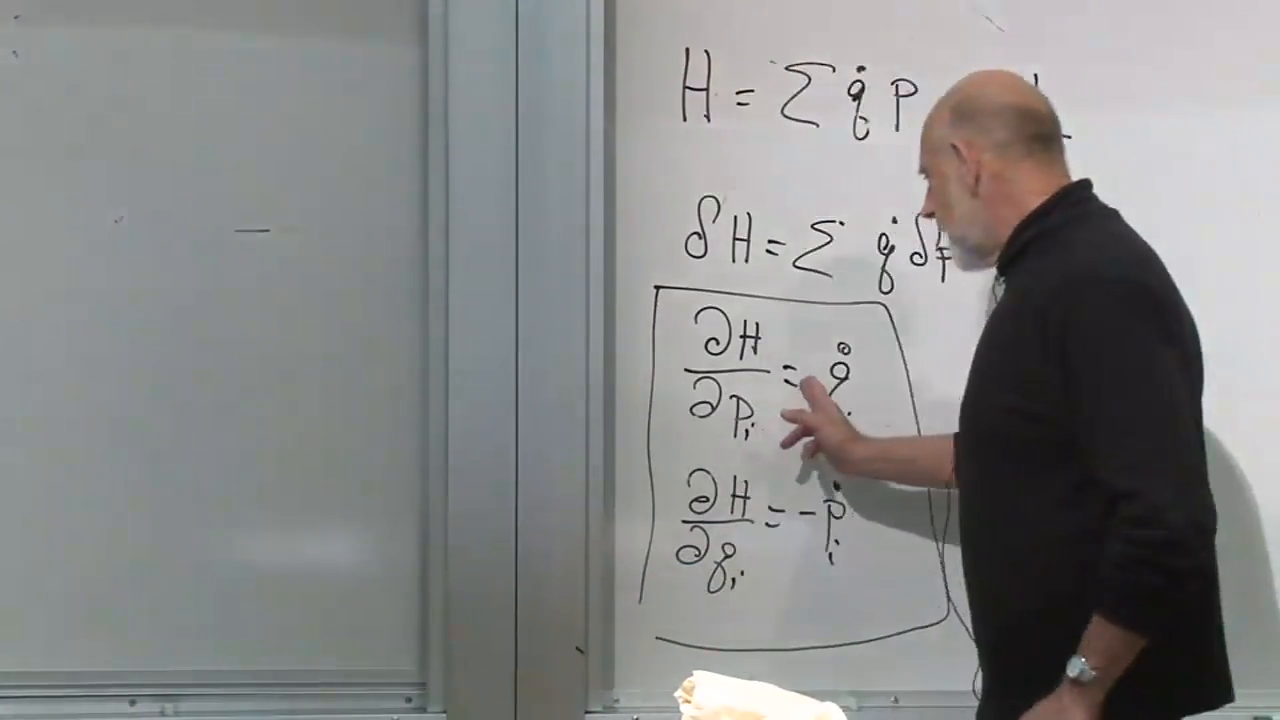
\includegraphics[width=0.78\textwidth]{lecture_06_figure_03.png}
  \caption{Définition de l’hamiltonien, sa variation et équations canoniques encadrées.}
  \lectureframe{01:22:18}
\end{figure}

Pour \(n\) coordonnées, ce sont \(2n\) équations du premier ordre. La formulation d’Euler--Lagrange fournit plutôt \(n\) équations du second ordre. La quantité de données initiales et le contenu physique sont identiques.

\section{Le mouvement de l’oscillateur comme rotation rigide}

En appliquant l’équation ~\eqref{eq:l6-hamilton-equations} à l’équation ~\eqref{eq:l6-oscillator-hamiltonian}, on obtient
\begin{equation}
  \dot q=\omega p,
  \qquad
  \dot p=-\omega q.
  \label{eq:l6-oscillator-first-order}
\end{equation}
En dérivant la première équation et en utilisant la seconde,
\begin{equation}
  \ddot q=\omega\dot p=-\omega^2q.
  \label{eq:l6-oscillator-second-order}
\end{equation}
Les deux équations du premier ordre sont donc exactement l’équation habituelle de l’oscillateur du second ordre, accompagnée de la définition du moment.

Dans l’espace des phases, le vecteur vitesse en \((q,p)\) est
\((\dot q,\dot p)=(\omega p,-\omega q)\), tangent au cercle d’énergie.
Tous les rayons tournent à la même vitesse angulaire \(\omega\). On peut imaginer le plan entier comme une hélice rigide ou comme un fluide fictif incompressible. Ses points circulent ; ils ne se contractent pas vers un puits et ne s’éloignent pas d’une source.

\begin{figure}[htbp]
  \centering
  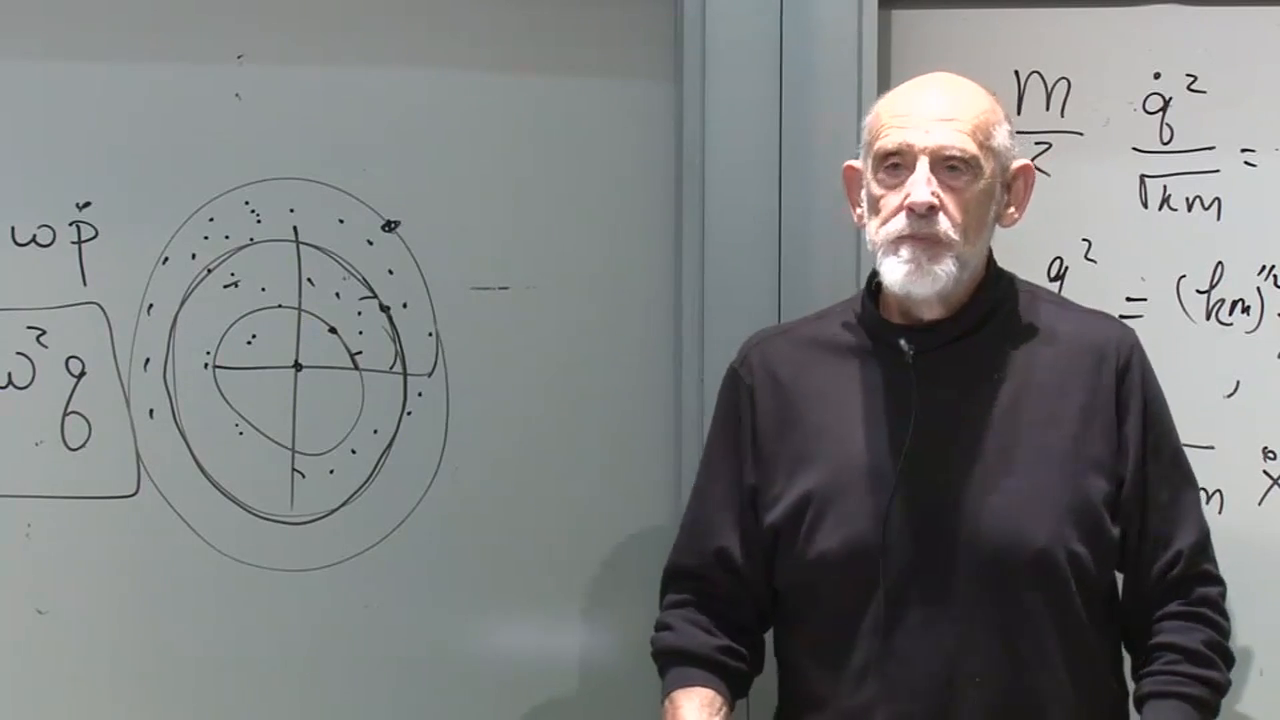
\includegraphics[width=0.86\textwidth]{lecture_06_figure_04.png}
  \caption{Nuage de points initiaux répartis sur des trajectoires emboîtées de l’espace des phases. L’évolution hamiltonienne déplace le nuage au lieu de le faire s’effondrer vers un état privilégié.}
  \lectureframe{01:39:27}
\end{figure}

\begin{figure}[htbp]
  \centering
  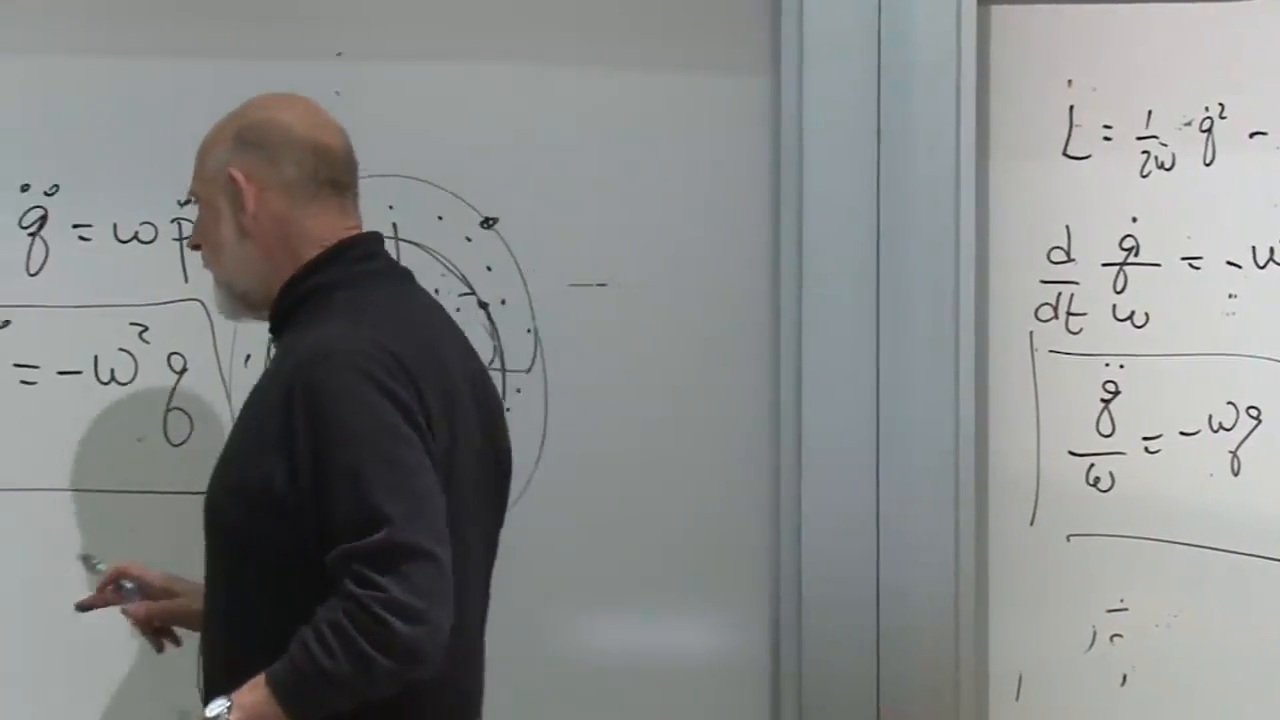
\includegraphics[width=0.90\textwidth]{lecture_06_figure_05.png}
  \caption{Portrait de phase de l’oscillateur, à côté de l’équation équivalente d’Euler--Lagrange
  \(\ddot q/\omega=-\omega q\).}
  \lectureframe{01:42:10}
\end{figure}

L’étape suivante consistera à transformer l’analogie du fluide en théorème : l’évolution hamiltonienne ne présente aucune convergence ni divergence locale. Ce résultat relie à nouveau la mécanique continue aux applications réversibles des états considérées au début du cours.

\section{Questions qui mettent en évidence le choix des coordonnées}

\begin{classroomqa}
  \audiencequestion{L’hypothèse selon laquelle on peut exprimer les vitesses en fonction de \(q\) et de \(p\) est-elle un théorème ou une propriété empirique des systèmes physiques ?
  \lecturetimestamp{01:29:08--01:29:45}}
  \lecturerresponse{Dans ce développement élémentaire, c’est une régularité empirique, qui trouve une motivation plus profonde en mécanique quantique. Plus précisément, la matrice jacobienne de l’équation ~\eqref{eq:l6-legendre-map} par rapport aux vitesses doit être non singulière. La mécanique moderne comprend aussi d’importants lagrangiens singuliers, notamment pour les systèmes contraints et de jauge, mais leur formulation hamiltonienne exige un traitement supplémentaire des contraintes.}
\end{classroomqa}

Une objection portant sur les unités explique pourquoi l’oscillateur a été écrit sous la forme inhabituelle de l’équation ~\eqref{eq:l6-rescaled-lagrangian}. Commençons plutôt par la coordonnée ordinaire \(x\) :
\begin{equation}
  L=\frac{m}{2}\dot x^2-\frac{k}{2}x^2,
  \qquad
  \omega=\sqrt{\frac{k}{m}}.
  \label{eq:l6-ordinary-oscillator}
\end{equation}
Choisissons
\begin{equation}
  q=(km)^{1/4}x.
  \label{eq:l6-oscillator-rescaling}
\end{equation}
On a alors \(q^2=\sqrt{km}\,x^2\) et
\(\dot q^2=\sqrt{km}\,\dot x^2\), ce qui transforme exactement l’équation ~\eqref{eq:l6-ordinary-oscillator} en l’équation ~\eqref{eq:l6-rescaled-lagrangian}. Le nouveau \(q\) est une coordonnée généralisée adaptée, et non une longueur ; son conjugué \(p\) n’est pas le moment mécanique ordinaire \(p_x=m\dot x\).

\begin{figure}[htbp]
  \centering
  \includegraphics[width=0.86\textwidth]{lecture_06_figure_15.png}
  \caption{Changement d’échelle dimensionnel de la coordonnée usuelle de l’oscillateur \(x\) vers la coordonnée adaptée \(q=(km)^{1/4}x\).}
  \lectureframe{01:36:10}
\end{figure}

\begin{classroomqa}
  \audiencequestion{Comment \(\omega p=\dot q\) peut-il être cohérent du point de vue dimensionnel, et pourquoi avoir choisi ces variables ?
  \lecturetimestamp{01:29:46--01:39:22}}
  \lecturerresponse{Le symbole \(q\) n’a pas nécessairement les dimensions d’une longueur, et son conjugué \(p\) n’a pas nécessairement les dimensions de \(m\dot x\). Le changement d’échelle de l’équation ~\eqref{eq:l6-oscillator-rescaling} préserve les dimensions du lagrangien et fait intervenir \(q\) et \(p\) de façon symétrique dans \(H\). Avec les variables d’origine,
  \[
    H=\frac{p_x^2}{2m}+\frac{kx^2}{2},
  \]
les courbes d’énergie constante dans le plan \((x,p_x)\) sont donc des ellipses. Dans le plan adapté \((q,p)\), ce sont des cercles. Le changement d’échelle a été choisi pour rendre cette symétrie visible.}
\end{classroomqa}

\begin{classroomqa}
  \audiencequestion{Comment des équations hamiltoniennes du premier ordre au nombre de \(2n\) peuvent-elles être équivalentes à des équations de Lagrange du second ordre au nombre de \(n\) ?
  \lecturetimestamp{01:39:24--01:42:30}}
  \lecturerresponse{Pour l’oscillateur, dérivons \(\dot q=\omega p\) et substituons \(\dot p=-\omega q\) ; on obtient le système \(\ddot q=-\omega^2q\). En partant directement du lagrangien, on trouve
  \[
    \frac{d}{dt}\left(\frac{\dot q}{\omega}\right)
      =-\omega q,
  \]
qui est la même équation du second ordre. On peut considérer qu’une équation de Hamilton définit le moment à partir de la vitesse, tandis que l’autre décrit l’évolution de ce moment.}
\end{classroomqa}

\section{Pourquoi l’espace des phases et l’énergie potentielle sont importants}

\begin{classroomqa}
  \audiencequestion{La puissance de la formulation hamiltonienne signifie-t-elle que l’espace des phases constitue une meilleure représentation géométrique que l’espace des configurations ?
  \lecturetimestamp{01:42:33--01:44:38}}
  \lecturerresponse{Ces deux espaces ont des fonctions différentes. L’espace des phases rend particulièrement visibles les cycles, les surfaces d’énergie constante et l’absence de convergence ou de divergence. Pour d’autres questions, l’espace des configurations peut être préférable. Si l’on insiste sur \(H\), c’est pour une raison plus profonde : cette quantité devient un objet central et plus intuitif en mécanique quantique, l’un des sujets modernes vers lesquels cette étude de la mécanique nous conduit.}
\end{classroomqa}

\begin{classroomqa}
  \audiencequestion{Faut-il considérer l’énergie potentielle comme l’intégrale de la force ?
  \lecturetimestamp{01:44:40--01:45:45}}
  \lecturerresponse{Pour les forces conservatives, cette affirmation est valable, à une constante près et avec le signe approprié. Il est plus utile de considérer le potentiel comme fondamental et d’en déduire la force généralisée :
  \[
    F_i=-\frac{\partial V}{\partial q_i}.
  \]
C’est précisément le terme qui apparaît dans \(\dot p_i=\partial L/\partial q_i\) lorsque \(L=T-V\) et que l’énergie cinétique ne dépend pas explicitement de \(q_i\).}
\end{classroomqa}

\begin{classroomqa}
  \audiencequestion{Quels problèmes de pointe cette voie vers la physique moderne est-elle censée éclairer ?
  \lecturetimestamp{01:45:46--01:47:47}}
  \lecturerresponse{Cette voie mène à la gravitation quantique et à la cosmologie ; à la physique des particules élémentaires, notamment au secteur de Higgs et aux neutrinos ; à la relativité ; à la théorie des cordes ; et à la théorie quantique des champs. Le problème théorique de fond reste de réunir ces éléments dans une structure cohérente, en particulier la mécanique quantique avec la gravitation, et la cosmologie avec la physique des particules. Il s’agissait d’un état des lieux des questions de pointe tel qu’il se présentait en 2011, et non de prétendre que leur solution était déjà connue.}
\end{classroomqa}

Les deux exemples avec contraintes et l’oscillateur s’inscrivent maintenant dans un même tableau. Les coordonnées généralisées éliminent les forces superflues. La symétrie sélectionne les moments canoniques conservés. La transformation de Legendre échange les vitesses contre les moments, et les équations de Hamilton décrivent la dynamique comme un flot dans l’espace des phases. Pour l’oscillateur, ce flot est une rotation rigide ; dans un système général, sa géométrie donnera un sens continu précis au mouvement réversible.
\chapter{Théorème de Liouville et flot hamiltonien}

\lectureoverview{Les équations de Hamilton ne se contentent pas de reformuler les équations du mouvement. Elles définissent un champ de vitesses dans l’espace des phases dont la divergence est nulle. Cette simple compensation constitue le théorème de Liouville : l’évolution hamiltonienne préserve le volume dans l’espace des phases. Nous allons y parvenir en suivant l’ordre qui en fait apparaître le sens---d’abord la conservation de l’énergie, puis les surfaces d’énergie constante, ensuite un fluide de conditions initiales possibles, et enfin le contraste entre un flot qui préserve le volume et un puits dissipatif. Ce même langage mène naturellement aux crochets de Poisson.}

\section{Pourquoi une autre formulation de la mécanique ?}

Le théorème que nous cherchons est l’équivalent classique continu des diagrammes d’états réversibles présentés au début du cours. Dans une loi discrète réversible, chaque état possède une flèche entrante et une flèche sortante. Le présent suffit à déterminer à la fois l’état suivant et l’état précédent. Une loi défectueuse envoie de nombreux états vers un même puits : l’avenir peut être déterminé, mais le passé n’est plus récupérable.

Le théorème de Liouville décrit ce qu’il advient de cette distinction lorsque l’ensemble des états est un espace des phases continu. L’expression qui remplace « une flèche entrante et une flèche sortante » est \emph{autant de flot entrant que de flot sortant}. Mais, avant de pouvoir lui donner un sens mathématique, nous devons reconstruire le flot à partir des équations de Hamilton.

Il y a là une énigme historique. Hamilton, Jacobi, Lagrange et Poisson ont élaboré des formulations complexes et remarquables de la mécanique classique sans connaître la théorie quantique, dans laquelle ces formulations allaient devenir indispensables. Newton avait un objectif concret : le mouvement des planètes. Lagrange et Hamilton avaient eux aussi des problèmes physiques à résoudre, mais ils ont exploré des analogies et des structures qui dépassaient largement le cadre d’une orbite particulière. L’action stationnaire en mécanique rappelait les principes du temps minimal en optique ; le mouvement des rayons et celui des particules pouvaient être exprimés dans des formes mathématiques parallèles. Ils simplifiaient, réorganisaient et unifiaient les équations parce que les structures elles-mêmes semblaient renfermer de la physique.

Nous savons aujourd’hui que cette intuition s’est révélée extraordinairement féconde. Sur le plan logique, de nombreux aspects de la mécanique classique peuvent se comprendre comme des limites de la mécanique quantique. Historiquement, l’ordre a été inverse : les structures classiques ont été découvertes en premier, et leur portée plus profonde n’est apparue que bien plus tard. Une plaisanterie provocatrice attribuée à Feynman faisait ressortir ce point en opposant les mathématiques poursuivies pour elles-mêmes à une physique contrainte par un partenaire extérieur : le monde physique. Cette plaisanterie n’est pas un argument, mais la distinction est utile : la beauté formelle compte ici parce que la nature fait sans cesse appel à ces structures formelles.

\begin{classroomqa}
  \audiencequestion{Newton avait-il la conception moderne de l’énergie cinétique, et
  d’où vient la notion d’énergie ?
  \lecturetimestamp{00:04:24--00:05:50}}
  \lecturerresponse{La mécanique de Newton s’organisait autour de la force et du mouvement,
  et non autour d’un principe général de conservation de l’énergie déjà abouti. La priorité historique exacte
  n’est pas tranchée dans la discussion. La \emph{vis viva} de Leibniz,
  \(\sum_i m_i v_i^2\), en fut un précurseur important et vaut deux fois l’énergie cinétique
  moderne. Les travaux ultérieurs sur la chaleur ont placé au premier plan sa conversion en travail mécanique.
  Les premières théories du calorique traitaient la chaleur comme une substance conservée ; l’idée moderne de formes
  d’énergie interchangeables ne s’est donc imposée que progressivement.}
\end{classroomqa}

\section{Équations de Hamilton et conservation de l’énergie}

Considérons un système doté de \(n\) paires canoniques,
\begin{equation}
  (q_i,p_i),\qquad i=1,\ldots,n.
  \label{eq:l7-canonical-pairs}
\end{equation}
À chaque coordonnée correspond une quantité de mouvement, et à chaque quantité de mouvement une coordonnée. La loi du mouvement est regroupée dans une seule fonction,
\begin{equation}
  H=H(q_1,\ldots,q_n,p_1,\ldots,p_n,t),
  \label{eq:l7-hamiltonian}
\end{equation}
et les équations de Hamilton s’écrivent
\begin{equation}
  \boxed{
  \dot q_i=\frac{\partial H}{\partial p_i},
  \qquad
  \dot p_i=-\frac{\partial H}{\partial q_i}.}
  \label{eq:l7-hamilton-equations}
\end{equation}
Le signe fait partie de la structure canonique. L’équation en \(q\) comporte le signe plus ; celle en \(p\) comporte le signe moins.

\begin{figure}[htbp]
  \centering
  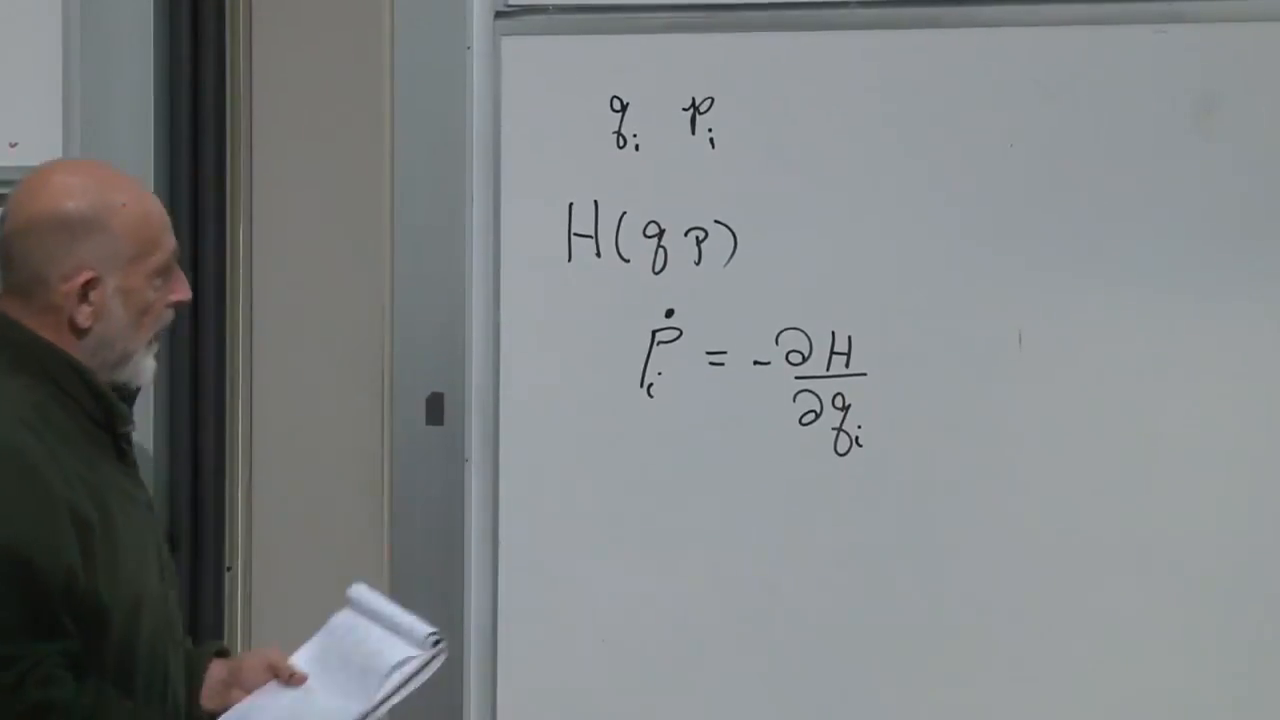
\includegraphics[width=0.82\textwidth]{lecture_07_figure_02.png}
  \caption{Les variables canoniques, la fonction \(H(q,p)\) et l’équation de Hamilton portant sur la quantité de mouvement, au début du récapitulatif.}
  \lectureframe{00:07:29}
\end{figure}

Bien que les équations soient organisées en paires indicées, la dynamique ne se sépare pas nécessairement paire par paire. Le Hamiltonien peut coupler tous les \(q_i\) et les \(p_i\) ; ainsi,
\(\dot p_1\), par exemple, peut dépendre de l’état du système tout entier.

\begin{classroomqa}
  \audiencequestion{La présentation est-elle maintenant axiomatique ? Quelle relation entre
  \(p\) et \(q\) a-t-on supposée ?
  \lecturetimestamp{00:17:08--00:18:18}}
  \lecturerresponse{Les équations de Hamilton définissent la théorie formelle dès lors que
  \(H(q,p)\) et les paires canoniques sont spécifiés. Il n’existe pas d’hypothèse supplémentaire
  universelle \(p=m\dot q\). Cette relation vaut pour une particule cartésienne ordinaire à énergie cinétique quadratique,
  mais d’autres coordonnées et d’autres Hamiltoniens donnent d’autres relations entre quantité de mouvement--et vitesse. Les équations elles-mêmes fournissent la relation par
  \(\dot q_i=\partial H/\partial p_i\). La question de savoir si un Hamiltonien proposé est réalisé dans la nature
  est une question physique distincte.}
\end{classroomqa}

Nous pouvons maintenant retrouver la conservation de l’énergie en un seul raisonnement. Le long d’une trajectoire, la dérivée totale de \(H\) vaut
\begin{equation}
  \frac{dH}{dt}
  =
  \sum_i\left(
    \frac{\partial H}{\partial q_i}\dot q_i
    +\frac{\partial H}{\partial p_i}\dot p_i
  \right)
  +\frac{\partial H}{\partial t}.
  \label{eq:l7-total-h-derivative}
\end{equation}
Le dernier terme représente la dépendance explicite en temps à \(q\) et \(p\) fixés, par exemple lorsqu’un paramètre imposé de l’extérieur varie. En substituant l’équation~\eqref{eq:l7-hamilton-equations},
\begin{align}
  \frac{dH}{dt}
  &=
  \sum_i\left[
    \frac{\partial H}{\partial q_i}
    \frac{\partial H}{\partial p_i}
    -\frac{\partial H}{\partial p_i}
    \frac{\partial H}{\partial q_i}
  \right]
  +\frac{\partial H}{\partial t}\\
  &=\frac{\partial H}{\partial t}.
  \label{eq:l7-h-energy-rate}
\end{align}
Chaque terme de la somme s’annule avec son correspondant. Par conséquent,
\begin{equation}
  \frac{\partial H}{\partial t}=0
  \quad\Longrightarrow\quad
  \frac{dH}{dt}=0.
  \label{eq:l7-energy-conservation}
\end{equation}
Pour un système fermé invariant par translation dans le temps, le Hamiltonien est conservé et correspond à l’énergie.

\begin{classroomqa}
  \audiencequestion{Que se passe-t-il si le Hamiltonien dépend explicitement du temps ? \lecturetimestamp{00:10:32--00:12:33}}
  \lecturerresponse{L’équation~\eqref{eq:l7-h-energy-rate} reste alors valable, mais l’énergie du sous-système
  n’est pas nécessairement constante. Une dépendance explicite en temps représente généralement un dispositif extérieur omis, qui échange de l’énergie avec le système. Si l’on inclut ce dispositif comme partie dynamique d’un système fermé plus vaste, le Hamiltonien global peut à nouveau être indépendant du temps et son énergie totale conservée.}
\end{classroomqa}

\section{L’énergie comme géométrie dans l’espace des phases}

Supposons maintenant que \(H\) ne dépende pas explicitement du temps. La condition initiale fixe une valeur \(E\), et le point représentatif dans l’espace des phases reste sur
\begin{equation}
  H(q,p)=E.
  \label{eq:l7-energy-surface}
\end{equation}
L’espace des phases a \(2n\) dimensions. Aux points réguliers, une équation entre ses coordonnées définit une hypersurface de dimension \((2n-1)\). Des valeurs différentes de \(E\) donnent des hypersurfaces différentes. Elles ne sont pas nécessairement fermées ou compactes ; la conservation de l’énergie signifie seulement qu’une trajectoire qui commence sur l’une d’elles ne la quitte jamais.

Pour l’oscillateur harmonique adapté du cours précédent,
\begin{equation}
  H=\frac{\omega}{2}(p^2+q^2).
  \label{eq:l7-oscillator-hamiltonian}
\end{equation}
Ainsi, chaque ensemble d’énergie constante est un cercle,
\begin{equation}
  p^2+q^2=\frac{2E}{\omega}.
  \label{eq:l7-oscillator-circle}
\end{equation}

\begin{figure}[htbp]
  \centering
  \includegraphics[width=0.84\textwidth]{lecture_07_figure_04.png}
  \caption{Schéma de l’espace des phases de dimension \(2n\) et Hamiltonien de l’oscillateur harmonique utilisés pour introduire les surfaces d’énergie constante.}
  \lectureframe{00:15:20}
\end{figure}

Les équations du mouvement,
\begin{equation}
  \dot q=\omega p,\qquad \dot p=-\omega q,
  \label{eq:l7-oscillator-flow}
\end{equation}
font tourner le point dans le sens horaire autour de son cercle. L’équation de l’énergie indique quelle courbe contient le mouvement ; les équations de Hamilton en donnent la direction et la vitesse le long de cette courbe.

\begin{figure}[htbp]
  \centering
  \begin{tikzpicture}[scale=0.95]
    \draw[->] (-2.7,0) -- (2.7,0) node[right] {\(q\)};
    \draw[->] (0,-2.7) -- (0,2.7) node[above] {\(p\)};
    \draw[thick] (0,0) circle (0.8);
    \draw[thick] (0,0) circle (1.5);
    \draw[thick] (0,0) circle (2.2);
    \draw[->,very thick] (0,2.2) arc[start angle=90,end angle=40,radius=2.2];
    \draw[->,very thick] (1.5,0) arc[start angle=0,end angle=-50,radius=1.5];
    \draw[->,very thick] (0,-0.8) arc[start angle=-90,end angle=-140,radius=0.8];
  \end{tikzpicture}
  \caption{L’énergie constante détermine les cercles ; les équations de l’oscillateur déterminent le champ tangent orienté dans le sens horaire.}
\end{figure}

\begin{classroomqa}
  \audiencequestion{Les deux équations de Hamilton et \(H=E\) sont-elles plusieurs formes d’une même équation ?
  \lecturetimestamp{00:15:53--00:17:06}}
  \lecturerresponse{Non. Les équations de Hamilton sont les deux lois du mouvement du premier ordre pour une paire canonique. Elles impliquent que \(dH/dt=0\), d’où découle \(H=E\). La valeur de \(E\) est déterminée par la condition initiale.
  L’équation \(H=E\) identifie une surface ; à elle seule, elle ne spécifie pas la vitesse le long de cette surface.}
\end{classroomqa}

\section{D’un état unique à un flot d’états}

Au lieu de suivre une seule condition initiale, parsemons l’espace des phases de toutes les conditions initiales possibles, puis lançons l’horloge. Chaque point représente un état possible complet, et chaque état évolue selon les équations de Hamilton. On peut imaginer cet ensemble comme une poussière ou un fluide fictif. Rien de matériel n’est versé dans l’espace des phases ; cette image du fluide permet de visualiser simultanément toutes les trajectoires.

Le champ de vitesses dans l’espace des phases est
\begin{equation}
  \mathbf V(q,p,t)
  =
  (\dot q_1,\ldots,\dot q_n,\dot p_1,\ldots,\dot p_n).
  \label{eq:l7-phase-velocity}
\end{equation}
Pour une seule paire canonique, nous écrivons
\begin{equation}
  V_q=\dot q=\frac{\partial H}{\partial p},
  \qquad
  V_p=\dot p=-\frac{\partial H}{\partial q}.
  \label{eq:l7-phase-components}
\end{equation}
En chaque point, le Hamiltonien attribue un vecteur qui indique au point représentatif où aller ensuite. Si \(H\) est indépendant du temps, le champ de vecteurs est stationnaire : lorsqu’on revient au même point de l’espace des phases, on retrouve la même vitesse. Si \(H\) dépend du temps, le champ lui-même varie au cours du temps, mais il reste défini à chaque instant.

\begin{figure}[htbp]
  \centering
  \includegraphics[width=0.84\textwidth]{lecture_07_figure_05.png}
  \caption{Le champ de vitesses de l’oscillateur harmonique. Les vecteurs sont tangents aux cercles et leur longueur diminue à mesure que l’on se rapproche de l’origine.}
  \lectureframe{00:24:50}
\end{figure}

Dans le cas de l’oscillateur harmonique, chaque rayon tourne à la vitesse angulaire \(\omega\). Les points proches de l’origine ont une vitesse linéaire plus faible, car ils parcourent un cercle plus petit pendant la même période. Toute la poussière tourne donc comme un carrousel rigide.

\begin{classroomqa}
  \audiencequestion{Une rotation rigide signifie-t-elle que toutes les trajectoires de l’oscillateur ont la même période ? \lecturetimestamp{00:21:10--00:21:42}}
  \lecturerresponse{Oui. L’indépendance par rapport à l’amplitude est la propriété caractéristique de l’oscillateur harmonique. Chaque cercle est parcouru avec la même pulsation \(\omega\), même si la norme de la vitesse dans l’espace des phases est plus faible sur un cercle plus petit.}
\end{classroomqa}

\begin{classroomqa}
  \audiencequestion{La vitesse dans l’espace des phases est-elle la même en tout point ?
  \lecturetimestamp{00:24:29--00:25:37}}
  \lecturerresponse{Non. Sa direction comme sa norme varient généralement avec la position. Pour l’oscillateur, le vecteur est tangent au cercle local et sa norme vaut \(\omega\sqrt{p^2+q^2}\). Un champ de vecteurs signifie qu’un vecteur est attribué à chaque point, et non qu’un même vecteur identique est reproduit partout.}
\end{classroomqa}

\begin{classroomqa}
  \audiencequestion{Que sont exactement les particules et la densité de ce fluide fictif ? \lecturetimestamp{00:56:03--00:58:40}}
  \lecturerresponse{Chaque point représente un état complet du système mécanique tout entier. Ce n’est pas une particule physique. Cinq particules se déplaçant dans une dimension spatiale requièrent cinq positions et cinq quantités de mouvement, donc un espace des phases à dix dimensions ; en trois dimensions, il en faut trente. La poussière représente un ensemble d’états possibles alternatifs. Si l’image du fluide vous gêne, considérez simplement une région de conditions initiales, faites évoluer chacun de ses points, puis comparez son volume dans l’espace des phases avant et après l’évolution.}
\end{classroomqa}

\section{Compression et divergence}

Pour savoir si ce fluide fictif perd du volume, commençons en une dimension. Des points sur une droite se déplacent avec la vitesse \(v(x)\). Deux points voisins séparés par \(\delta x\) présentent une différence de vitesse égale à
\begin{equation}
  \delta v \simeq \frac{dv}{dx}\,\delta x.
  \label{eq:l7-one-dimensional-strain}
\end{equation}
Si \(dv/dx>0\), le point situé devant se déplace plus vite et l’intervalle s’étire. Si \(dv/dx<0\), il se comprime. Un flot stationnaire incompressible à une dimension vérifie donc
\begin{equation}
  \frac{dv}{dx}=0.
  \label{eq:l7-one-dimensional-incompressible}
\end{equation}

\begin{figure}[htbp]
  \centering
  \includegraphics[width=0.84\textwidth]{lecture_07_figure_06.png}
  \caption{Construction en une dimension menant à \(dv/dx\) comme taux local d’étirement ou de compression.}
  \lectureframe{00:30:20}
\end{figure}

Deux points de vue équivalents sont possibles. Nous pouvons suivre un intervalle matériel et demander si sa longueur change. Ou bien nous pouvons maintenir un petit intervalle fixe et demander si la quantité qui y entre par unité de temps est égale à celle qui en sort. Le premier point de vue suit le fluide ; le second le voit passer.

En dimension supérieure, une région peut s’étirer le long d’un axe et se comprimer le long d’un autre sans que son volume total change. Pour un champ de vitesses \(\mathbf V=(V_x,V_y,V_z)\), le taux local pertinent est la divergence,
\begin{equation}
  \nabla\cdot\mathbf V
  =
  \frac{\partial V_x}{\partial x}
  +\frac{\partial V_y}{\partial y}
  +\frac{\partial V_z}{\partial z}.
  \label{eq:l7-spatial-divergence}
\end{equation}
Une divergence positive correspond à une expansion locale, une divergence négative à une contraction locale, et l’incompressibilité à
\begin{equation}
  \nabla\cdot\mathbf V=0.
  \label{eq:l7-zero-divergence}
\end{equation}
L’égalité des flux entrant et sortant à travers une petite boîte fixe exprime localement la même chose que la conservation du volume d’une petite boîte en mouvement.

\begin{figure}[htbp]
  \centering
  \includegraphics[width=0.86\textwidth]{lecture_07_figure_07.png}
  \caption{Boîte bidimensionnelle, composantes du flot et somme des dérivées par rapport aux coordonnées correspondantes qui définit la divergence.}
  \lectureframe{00:35:30}
\end{figure}

\begin{classroomqa}
  \audiencequestion{Parlons-nous d’un fluide dans l’espace ordinaire ou d’un flot dans l’espace des phases ? \lecturetimestamp{00:34:27--00:34:40}}
  \lecturerresponse{L’argument sur la divergence est d’abord un argument général sur les fluides. Nous l’appliquerons à l’espace des phases, de dimension paire, dont les directions de coordonnées sont les \(q_i\) et les \(p_i\), et dont les composantes de vitesse sont les \(\dot q_i\) et les \(\dot p_i\).}
\end{classroomqa}

Revenons maintenant aux applications discrètes entre états. Dans un cycle réversible, chaque nœud possède une flèche entrante et une flèche sortante, et un ensemble choisi d’états conserve le même nombre d’éléments au cours de son évolution. Dans un puits, de nombreuses flèches entrent et trop peu en sortent ; plusieurs possibilités deviennent indiscernables.

\begin{figure}[htbp]
  \centering
  \includegraphics[width=0.80\textwidth]{lecture_07_figure_08.png}
  \caption{Le puits discret qui relie la divergence au critère des lois réversibles présenté dans la première leçon.}
  \lectureframe{00:40:15}
\end{figure}

La question continue est maintenant précise : le flot hamiltonien a-t-il une divergence nulle, de sorte qu’une petite région d’états discernables ne soit jamais réduite à un volume plus petit dans l’espace des phases ?

\section{Théorème de Liouville}

\begin{theorem}[Liouville's theorem]Pour un système hamiltonien régulier, le champ canonique de vitesses dans l’espace des phases est de divergence nulle :
\begin{equation}
  \sum_i\left(
    \frac{\partial\dot q_i}{\partial q_i}
    +\frac{\partial\dot p_i}{\partial p_i}
  \right)=0.
  \label{eq:l7-liouville-divergence}
\end{equation}
De façon équivalente, l’évolution hamiltonienne préserve l’élément de volume canonique dans l’espace des phases
\(dq_1\cdots dq_n\,dp_1\cdots dp_n\).
\end{theorem}

\begin{classroomqa}
  \audiencequestion{Les composantes notées \(V\) sont-elles simplement les dérivées temporelles de \(p\) et de \(q\) ? \lecturetimestamp{00:42:20--00:43:22}}
  \lecturerresponse{Oui. Pour une paire,
  \(V_q=\dot q\) et \(V_p=\dot p\). En réunissant toutes ces dérivées, on obtient le vecteur vitesse du flot dans l’espace des phases tout entier.}
\end{classroomqa}

Pour une paire canonique, les équations de Hamilton donnent
\begin{equation}
  V_p=-\frac{\partial H}{\partial q},
  \qquad
  V_q=\frac{\partial H}{\partial p}.
  \label{eq:l7-liouville-components}
\end{equation}
La divergence vaut donc
\begin{align}
  \frac{\partial V_p}{\partial p}
  +\frac{\partial V_q}{\partial q}
  &=
  -\frac{\partial}{\partial p}
    \left(\frac{\partial H}{\partial q}\right)
  +\frac{\partial}{\partial q}
    \left(\frac{\partial H}{\partial p}\right)\\
  &=
  -\frac{\partial^2H}{\partial p\,\partial q}
  +\frac{\partial^2H}{\partial q\,\partial p}
  =0.
  \label{eq:l7-liouville-proof}
\end{align}

\begin{figure}[htbp]
  \centering
  \includegraphics[width=0.86\textwidth]{lecture_07_figure_09.png}
  \caption{Rectangle de différences finies utilisé pour expliquer pourquoi les dérivées partielles mixtes de fonctions régulières commutent.}
  \lectureframe{00:47:30}
\end{figure}

L’égalité des dérivées partielles mixtes se voit en considérant quatre points voisins \(A,B,C,D\) aux sommets d’un petit rectangle dans le plan \(q\)-\(p\). Calculer une différence selon \(q\), puis une différence selon \(p\), donne, à un facteur égal au produit des deux petits côtés près,
\begin{equation}
  F(B)+F(D)-F(A)-F(C).
  \label{eq:l7-finite-difference-combination}
\end{equation}
Prendre les différences dans l’ordre inverse donne la même combinaison. À la limite d’un rectangle infiniment petit, on obtient
\(\partial_p\partial_qF=\partial_q\partial_pF\), à condition que les dérivées requises soient continues.

\begin{figure}[htbp]
  \centering
  \includegraphics[width=0.88\textwidth]{lecture_07_figure_10.png}
  \caption{La divergence canonique, une fois les équations de Hamilton ramenées à deux dérivées mixtes de signes opposés.}
  \lectureframe{00:50:20}
\end{figure}

Pour de nombreux degrés de liberté, la même compensation se produit pour chaque paire canonique :
\begin{align}
  \sum_i\left(
    \frac{\partial\dot p_i}{\partial p_i}
    +\frac{\partial\dot q_i}{\partial q_i}
  \right)
  &=
  \sum_i\left(
    -\frac{\partial^2H}{\partial p_i\,\partial q_i}
    +\frac{\partial^2H}{\partial q_i\,\partial p_i}
  \right)\\
  &=0.
  \label{eq:l7-many-pair-proof}
\end{align}
L’étirement dans une direction canonique est compensé par la compression dans la direction qui lui est conjuguée. Cette compensation paire par paire est une structure plus forte qu’une annulation fortuite entre des axes sans lien.

\begin{classroomqa}
  \audiencequestion{La somme porte-t-elle implicitement sur toutes les paires canoniques ?
  \lecturetimestamp{00:52:00--00:52:36}}
  \lecturerresponse{Oui. L’équation~\eqref{eq:l7-many-pair-proof} est sommée sur \(i\), et les deux dérivées mixtes s’annulent séparément pour chaque paire \(q_i,p_i\).}
\end{classroomqa}

\begin{classroomqa}
  \audiencequestion{La divergence affichée semble écrite en coordonnées cartésiennes. Le théorème reste-t-il valable après un changement de coordonnées ?
  \lecturetimestamp{00:52:50--00:53:22,\allowbreak\ 00:58:18--00:58:40}}
  \lecturerresponse{L’énoncé naturel se formule en coordonnées canoniques et avec l’élément de volume canonique
  \(dq_1\cdots dq_n\,dp_1\cdots dp_n\). Une transformation canonique, ou symplectique, change simultanément les coordonnées et les quantités de mouvement, tout en préservant ce volume. En coordonnées non canoniques arbitraires, la mesure de volume doit inclure un facteur jacobien ; le produit naïf des accroissements des coordonnées n’est pas nécessairement invariant.}
\end{classroomqa}

\begin{classroomqa}
  \audiencequestion{Le théorème de Liouville exige-t-il un Hamiltonien indépendant du temps ? \lecturetimestamp{00:53:43--00:55:51}}
  \lecturerresponse{Non. La conservation de l’énergie exigeait que \(\partial H/\partial t=0\), mais, dans la démonstration de la divergence, les dérivées sont prises uniquement par rapport à \(q_i\) et \(p_i\) à un instant fixé. Les dérivées mixtes s’annulent toujours pour \(H(q,p,t)\). Un Hamiltonien dépendant du temps engendre donc un flot canonique dépendant du temps, mais qui préserve le volume à chaque instant.}
\end{classroomqa}

\section{Ce que signifie, et ne signifie pas, la conservation du volume}

Prenons une petite région \(R_0\) de conditions initiales et faisons évoluer chacun de ses points pendant une durée \(t\). Le théorème de Liouville affirme que
\begin{equation}
  \operatorname{Vol}(R_t)=\operatorname{Vol}(R_0).
  \label{eq:l7-volume-preservation}
\end{equation}
La région peut se déplacer, tourner, subir un cisaillement et s’étirer en un long filament. C’est son volume, et non sa forme, qui est préservé. Dans une évolution hamiltonienne régulière de durée finie, des points distincts de l’espace des phases ne peuvent pas fusionner.

Pour des durées finies, un flot hamiltonien régulier définit une application inversible, dont l’inverse régulier s’obtient en faisant évoluer le système à rebours. Cela explique aussi l’affirmation faite en cours selon laquelle une masse connexe ne peut pas se pincer au point de se scinder en morceaux disjoints : le flot déforme continûment la région et en préserve la topologie, même si un col extrêmement fin peut donner l’impression, à résolution finie, que deux lobes sont séparés.

\begin{figure}[htbp]
  \centering
  \includegraphics[width=0.86\textwidth]{lecture_07_figure_12.png}
  \caption{Déformations possibles d’une région de l’espace des phases. Un flot hamiltonien régulier peut créer un col fin, mais pas une véritable scission en morceaux évoluant indépendamment en un temps fini.}
  \lectureframe{01:04:55}
\end{figure}

\begin{classroomqa}
  \audiencequestion{Une région de l’espace des phases peut-elle se pincer puis se scinder en deux morceaux ? \lecturetimestamp{01:04:10--01:05:49}}
  \lecturerresponse{Pas sous l’effet d’un flot hamiltonien régulier et déterministe pendant un temps fini. Au point de pincement hypothétique, il y a toujours un seul point de l’espace des phases et un seul vecteur vitesse qui lui est attribué, et non deux directions incompatibles. La région peut développer un filament de connexion très long et très étroit, mais l’évolution reste bijective et ne le déchire pas.}
\end{classroomqa}

\begin{classroomqa}
  \audiencequestion{Deux lobes très éloignés d’une masse étirée sont-ils physiquement reliés ou intriqués quantiquement ?
  \lecturetimestamp{01:08:01--01:09:16}}
  \lecturerresponse{Aucune connexion physique de ce type n’est impliquée. La masse représente un ensemble de conditions initiales possibles, et non un objet matériel unique. Dire qu’il s’agit d’une seule région indique que ces états proviennent du même ensemble initial ; cela ne dit rien sur d’éventuelles forces ou intrications quantiques entre eux.}
\end{classroomqa}

\begin{classroomqa}
  \audiencequestion{Que se passe-t-il près de la position d’équilibre instable verticale d’un pendule rigide ? Les trajectoires dans le sens horaire et dans le sens antihoraire se chevauchent-elles ?
  \lecturetimestamp{01:07:07--01:07:47}}
  \lecturerresponse{Des conditions initiales voisines peuvent diverger vers des trajectoires très différentes, produisant les filaments fins décrits plus haut. Elles ne deviennent pas le même point de l’espace des phases : le signe du déplacement infinitésimal ou de la quantité de mouvement distingue les deux côtés. L’état parfaitement équilibré suit son propre mouvement, déterminé de façon unique : dans le modèle idéal, il reste à l’équilibre.}
\end{classroomqa}

\subsection{Expansion dans l’espace des positions et contraction dans l’espace des quantités de mouvement}

Si une transformation canonique dilate un intervalle de positions d’un facteur \(a\), l’échelle de la quantité de mouvement conjuguée se contracte du facteur réciproque :
\begin{equation}
  q\longrightarrow aq,
  \qquad
  p\longrightarrow \frac{p}{a},
  \qquad
  dq\,dp\longrightarrow dq\,dp.
  \label{eq:l7-canonical-scaling}
\end{equation}
Voilà le contenu précis, dans l’espace des phases, qui sous-tend l’exemple de la détente d’un gaz. Lors d’une détente adiabatique, la région accessible dans l’espace ordinaire s’agrandit, tandis que les quantités de mouvement typiques diminuent et que le gaz se refroidit. La relation thermodynamique détaillée dépend de la dimension, du protocole de détente et des interactions ; le théorème de Liouville impose la contrainte sur le volume, mais ne donne pas tous les coefficients thermodynamiques.

\begin{classroomqa}
  \audiencequestion{Le même raisonnement s’applique-t-il à l’expansion de l’Univers, même si elle est soudaine ? \lecturetimestamp{00:53:23--00:56:00}}
  \lecturerresponse{Le théorème de Liouville s’applique dès lors que la dynamique complète est hamiltonienne, y compris lorsque les variables canoniques dépendent explicitement du temps. Une expansion selon les directions de position doit s’accompagner de la contraction correspondante selon les directions des quantités de mouvement canoniques. Toutefois, le facteur d’échelle cosmologique, une détente contrôlée d’un gaz et l’explosion libre d’un nuage ne correspondent pas au même processus physique. Une corrélation de type Hubble entre la distance et la vitesse d’éloignement peut apparaître parce que les objets les plus rapides parcourent une plus grande distance, tandis que le refroidissement adiabatique concerne la contraction de la distribution locale des quantités de mouvement. Dans chaque cas, le théorème contraint l’application complète dans l’espace des phases.}
\end{classroomqa}

\begin{classroomqa}
  \audiencequestion{À quoi sert concrètement le théorème de Liouville ?
  \lecturetimestamp{01:06:16--01:07:04}}
  \lecturerresponse{Il joue un rôle central en mécanique statistique. Il détermine l’évolution des ensembles d’états microscopiques et sous-tend la relation entre le volume dans l’espace des phases et l’entropie. La détente et le refroidissement d’un gaz en fournissent un exemple immédiat ; par la suite, le théorème devient un outil fondamental pour raisonner sur l’équilibre et le hors-équilibre.}
\end{classroomqa}

\section{Un flot qui déforme fortement les formes}

L’oscillateur harmonique préserve à la fois l’aire et la forme, car son flot est une rotation rigide. C’est un cas exceptionnel. Pour distinguer conservation du volume et rigidité, considérons
\begin{equation}
  H=\lambda pq,
  \label{eq:l7-pq-hamiltonian}
\end{equation}
où \(\lambda\) a la dimension de l’inverse d’un temps. Dans le cours, on pose
\(\lambda=1\) ; le conserver permet d’expliciter les dimensions.

\begin{figure}[htbp]
  \centering
  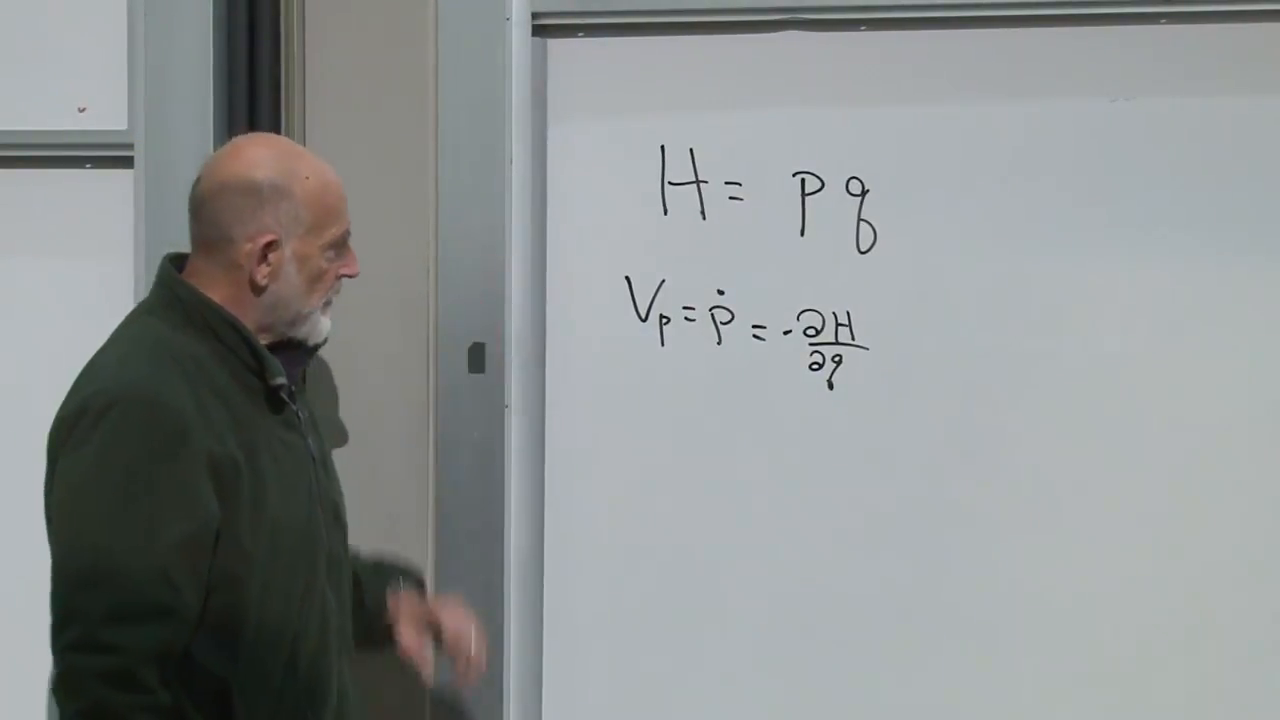
\includegraphics[width=0.82\textwidth]{lecture_07_figure_03.png}
  \caption{Début de l’exemple \(H=pq\) et première composante de la vitesse dans l’espace des phases.}
  \lectureframe{01:00:11}
\end{figure}

Les équations de Hamilton sont
\begin{equation}
  \dot p=-\lambda p,
  \qquad
  \dot q=\lambda q,
  \label{eq:l7-pq-flow}
\end{equation}
et leurs solutions sont
\begin{equation}
  p(t)=p_0e^{-\lambda t},
  \qquad
  q(t)=q_0e^{\lambda t}.
  \label{eq:l7-pq-solutions}
\end{equation}
Un carré est comprimé exponentiellement selon \(p\) et étiré du même facteur selon \(q\) :
\begin{equation}
  \Delta p(t)\Delta q(t)
  =
  \Delta p(0)\Delta q(0).
  \label{eq:l7-pq-area}
\end{equation}
Sa divergence confirme localement le résultat,
\begin{equation}
  \frac{\partial\dot p}{\partial p}
  +\frac{\partial\dot q}{\partial q}
  =-\lambda+\lambda=0.
  \label{eq:l7-pq-divergence}
\end{equation}

\begin{figure}[htbp]
  \centering
  \includegraphics[width=0.86\textwidth]{lecture_07_figure_11.png}
  \caption{Une région compacte étirée en une longue bande mince, tandis que l’aire est préservée par le flot \(H=pq\).}
  \lectureframe{01:02:10}
\end{figure}

\begin{classroomqa}
  \audiencequestion{Puisque \(pq\) a la dimension d’une action, le théorème de Liouville exprime-t-il la conservation de l’action ? \lecturetimestamp{01:03:00--01:04:09}}
  \lecturerresponse{Non. Le théorème exprime la conservation du volume dans l’espace des phases. Pour une paire canonique, \(dq\,dp\) a la dimension d’une action, ce qui annonce la mécanique quantique, où les cellules de l’espace des phases se mesurent en unités déterminées par \(\hbar\). Mais le produit \(pq\) n’est pas en soi la fonctionnelle d’action de Hamilton, et il ne représente pas automatiquement un moment cinétique simplement parce que les dimensions coïncident.}
\end{classroomqa}

Cet exemple montre aussi que les angles ne sont pas nécessairement préservés. Une croix à angle droit, dont les composantes sont inégales, subit un cisaillement dans son aspect métrique lors de la mise à l’échelle décrite par l’équation~\eqref{eq:l7-pq-solutions}, alors que l’aire reste inchangée. Le théorème de Liouville porte sur l’aire ou le volume, et non sur la rigidité au sens de la géométrie euclidienne ordinaire.

\section{L’amortissement crée un puits}

Pour voir ce que le théorème exclut, considérons l’équation réduite d’un oscillateur amorti,
\begin{equation}
  m\ddot x=-kx-c\dot x,
  \qquad c>0.
  \label{eq:l7-damped-newton}
\end{equation}
Posons \(p=m\dot x\). Alors,
\begin{equation}
  \dot x=\frac{p}{m},
  \qquad
  \dot p=-kx-\frac{c}{m}p.
  \label{eq:l7-damped-first-order}
\end{equation}
Sans amortissement, le point représentatif dans l’espace des phases décrit des cercles autour de l’origine. Avec l’amortissement, l’énergie est transférée aux degrés de liberté microscopiques du milieu environnant, et la trajectoire spirale vers l’intérieur.

\begin{figure}[htbp]
  \centering
  \includegraphics[width=0.84\textwidth]{lecture_07_figure_13.png}
  \caption{Équation de l’oscillateur amorti et spirale convergeant vers l’origine dans le plan \(x\)-\(p\).}
  \lectureframe{01:13:30}
\end{figure}

La divergence de ce flot réduit à deux dimensions vaut
\begin{equation}
  \frac{\partial\dot x}{\partial x}
  +\frac{\partial\dot p}{\partial p}
  =
  0-\frac{c}{m}<0.
  \label{eq:l7-damped-divergence}
\end{equation}
Toute région de taille finie se contracte. L’origine est un puits, l’analogue continu de l’application entre états où plusieurs flèches convergent vers un même état.

\begin{figure}[htbp]
  \centering
  \includegraphics[width=0.88\textwidth]{lecture_07_figure_14.png}
  \caption{Composantes de la vitesse dans l’espace des phases de l’oscillateur amorti, utilisées pour obtenir la divergence négative \(-c/m\).}
  \lectureframe{01:16:05}
\end{figure}

Cela ne signifie pas que la mécanique microscopique viole le théorème de Liouville. Les deux variables \(x,p\) laissent de côté l’énorme nombre de degrés de liberté de l’environnement qui reçoivent l’énergie de l’oscillateur. Le système élargi, formé de l’oscillateur et de son environnement, peut être hamiltonien et préserver le volume, même si sa description réduite \(x,p\) implique une contraction.

\begin{classroomqa}
  \audiencequestion{L’oscillateur amorti est-il toujours décrit par l’équation de Newton, même s’il n’est pas hamiltonien dans cet espace des phases réduit ?
  \lecturetimestamp{01:20:09--01:21:12}}
  \lecturerresponse{Oui. La loi \(F=ma\) peut inclure une force de frottement déterminée empiriquement. La description élémentaire fondée sur \(L=T-V\) et la formulation hamiltonienne s’appliquent directement aux forces conservatives ; des lagrangiens plus généraux permettent aussi de traiter certaines forces dépendant de la vitesse. Un terme de frottement markovien pour un système isolé décrit par le couple \(x,p\) relève toutefois d’une dynamique dissipative réduite, et non d’un système hamiltonien canonique fermé.}
\end{classroomqa}

\begin{classroomqa}
  \audiencequestion{Si l’on peut intégrer les équations de l’oscillateur amorti à rebours avec une précision infinie, l’information est-elle vraiment perdue ?
  \lecturetimestamp{01:25:16--01:27:17}}
  \lecturerresponse{Pour tout temps fini, l’équation différentielle idéale admet encore une application inverse : on peut donc remonter le temps à partir de données exactes. L’énoncé précis est que les cellules finies de l’espace des phases se contractent exponentiellement. Pour retrouver leur passé, il faut alors une précision qui augmente exponentiellement ; à temps infini, toutes les trajectoires convergent vers le puits. C’est l’analogue classique continu le plus proche de l’image discrète de la perte de possibilités, et non l’affirmation que deux solutions exactes à temps fini deviennent littéralement une seule.}
\end{classroomqa}

\begin{classroomqa}
  \audiencequestion{Un champ vectoriel peut-il avoir une divergence nulle sans être issu d’un hamiltonien ? \lecturetimestamp{01:18:21--01:22:34}}
  \lecturerresponse{Certainement. La formulation hamiltonienne suffit à assurer une divergence nulle, mais elle n’est pas nécessaire. Un champ de vitesse incompressible quelconque peut avoir une divergence nulle sans être un champ hamiltonien canonique sur ce même espace. Le champ de vitesse d’un fluide incompressible en trois dimensions en est l’exemple classique : trois coordonnées ne peuvent pas, à elles seules, former des paires canoniques. La mécanique complète des fluides peut admettre des formulations hamiltoniennes plus élaborées, en dimension infinie, mais cela ne renverse pas l’implication à sens unique énoncée ici.}
\end{classroomqa}

\section{D’autres distinctions mises en lumière par les questions}

\begin{classroomqa}
  \audiencequestion{Quel est le lien entre le mouvement sur une surface d’énergie constante et la préservation du volume de tout l’espace des phases ?
  \lecturetimestamp{01:28:47--01:30:41}}
  \lecturerresponse{Ce sont des conséquences indépendantes de la structure hamiltonienne. Si \(H\) ne dépend pas explicitement du temps, chaque trajectoire reste sur sa propre surface d’énergie. Une portion finie peut traverser plusieurs de ces surfaces ; le théorème de Liouville affirme que le volume de cette portion entière est préservé. Dans le cas de l’oscillateur harmonique, la portion conserve aussi sa forme, car le flot est une rotation rigide. La portion \(H=pq\) ne conserve que son aire, et non sa forme.}
\end{classroomqa}

\begin{classroomqa}
  \audiencequestion{Quelle place le travail mécanique occupe-t-il dans la formulation hamiltonienne ? \lecturetimestamp{01:30:44--01:32:57}}
  \lecturerresponse{Le travail décrit un transfert d’énergie à travers la frontière choisie d’un système. Un agent extérieur peut soulever un poids ou modifier un paramètre et ainsi changer l’énergie du sous-système ; l’agent perd alors l’énergie qu’il fournit. Si les deux parties sont incluses dans un même modèle fermé, l’accent revient à la conservation de l’énergie totale et aux échanges entre sous-systèmes.}
\end{classroomqa}

\begin{classroomqa}
  \audiencequestion{La préservation du volume implique-t-elle aussi celle de la topologie et des angles ? \lecturetimestamp{01:33:00--01:33:37}}
  \lecturerresponse{Un flot hamiltonien régulier à temps fini préserve la topologie, car il s’agit d’une déformation continue inversible. En général, il ne préserve ni les angles euclidiens ni la forme. La rotation rigide de l’oscillateur les préserve, mais l’étirement dans le cas \(H=pq\) montre pourquoi ce cas est particulier.}
\end{classroomqa}

\begin{classroomqa}
  \audiencequestion{La transformation de Legendre a-t-elle été omise parce qu’elle n’a aucune signification physique ? \lecturetimestamp{01:33:43--01:34:48}}
  \lecturerresponse{Non. C’est la transformation utile qui remplace la description en termes de vitesse par celle en termes de quantité de mouvement et qui produit \(H=\sum_i p_i\dot q_i-L\) lorsque l’application est régulière. Cette construction a déjà été utilisée à plusieurs reprises, même si son nom formel n’a pas été souligné ; la théorie générale détaillée n’est tout simplement pas nécessaire pour le théorème étudié ici.}
\end{classroomqa}

\section{Crochets de Poisson : une nouvelle condensation}

Les dernières minutes reviennent au thème historique. Au XIXe siècle, la mécanique a cherché à plusieurs reprises des structures concises reliant des systèmes apparemment différents --- la mécanique et l’optique géométrique, les particules et les rayons, les trajectoires classiques et les descriptions ondulatoires. Les crochets de Poisson constituent une autre structure de ce type, qui prend une importance particulière en mécanique quantique.

Soit \(F(q,p)\) une fonction quelconque de l’espace des phases. Il peut s’agir d’une coordonnée, d’une quantité de mouvement, du produit \(qp\) ou du moment cinétique. Au cours du mouvement,
\begin{equation}
  \frac{dF}{dt}
  =
  \sum_i\left(
    \frac{\partial F}{\partial q_i}\dot q_i
    +\frac{\partial F}{\partial p_i}\dot p_i
  \right).
  \label{eq:l7-f-time-derivative}
\end{equation}
Substituons les équations de Hamilton :
\begin{equation}
  \frac{dF}{dt}
  =
  \sum_i\left(
    \frac{\partial F}{\partial q_i}
    \frac{\partial H}{\partial p_i}
    -
    \frac{\partial F}{\partial p_i}
    \frac{\partial H}{\partial q_i}
  \right).
  \label{eq:l7-f-hamiltonian-derivative}
\end{equation}

\begin{figure}[htbp]
  \centering
  \includegraphics[width=0.88\textwidth]{lecture_07_figure_15.png}
  \caption{Règle de dérivation en chaîne pour la dérivée temporelle d’une fonction générale de l’espace des phases \(F(q,p)\).}
  \lectureframe{01:42:40}
\end{figure}

La combinaison antisymétrique qui revient ici mérite un nom. Pour deux fonctions quelconques \(F\) et \(G\), définissons leur crochet de Poisson par
\begin{equation}
  \boxed{
  \{F,G\}
  =
  \sum_i\left(
    \frac{\partial F}{\partial q_i}
    \frac{\partial G}{\partial p_i}
    -
    \frac{\partial F}{\partial p_i}
    \frac{\partial G}{\partial q_i}
  \right).}
  \label{eq:l7-poisson-bracket}
\end{equation}

\begin{figure}[htbp]
  \centering
  \includegraphics[width=0.86\textwidth]{lecture_07_figure_16.png}
  \caption{La combinaison de dérivées de deux fonctions, élevée au rang de crochet de Poisson.}
  \lectureframe{01:44:15}
\end{figure}

L’équation~\eqref{eq:l7-f-hamiltonian-derivative} devient
\begin{equation}
  \boxed{\frac{dF}{dt}=\{F,H\}.}
  \label{eq:l7-hamiltonian-poisson-evolution}
\end{equation}
Si \(F\) dépend aussi explicitement du temps, on ajoute \(\partial F/\partial t\). En prenant \(F=q_i\) ou \(F=p_i\), on retrouve les deux équations de Hamilton ; l’équation~\eqref{eq:l7-hamiltonian-poisson-evolution} constitue donc une formulation compacte de la dynamique complète.

On peut toujours condenser artificiellement la notation---on pourrait mettre au carré plusieurs équations, les additionner et appeler le résultat une seule équation. Cela masquerait la structure au lieu de la révéler. Le crochet de Poisson est utile pour la raison inverse : son algèbre organise l’évolution temporelle, les quantités conservées et les symétries. L’étape suivante consiste à développer cette algèbre, puis à l’appliquer au moment cinétique, dont la structure sera centrale en mécanique classique comme en théorie quantique.

\section{Le sens continu de la réversibilité}

Nous pouvons maintenant exposer toute la chaîne d’idées, sans la raccourcir. Les équations de Hamilton conservent \(H\) lorsque l’hamiltonien ne dépend pas explicitement du temps ; les trajectoires individuelles restent donc sur des hypersurfaces d’énergie constante. Ces mêmes équations attribuent une vitesse à chaque point de l’espace des phases. La divergence de ce champ de vitesse est nulle, car les dérivées partielles mixtes s’annulent deux à deux. Par conséquent, une région entière d’états possibles conserve son volume canonique.

C’est la version continue du principe « une flèche entrante, une flèche sortante ». La forme peut changer, les angles peuvent changer et des trajectoires voisines peuvent s’écarter considérablement. Dans une formulation hamiltonienne fermée et régulière, ce qui ne peut pas se produire, c’est la compression d’un ensemble fini de possibilités en un volume plus petit de l’espace des phases. Le flot \(H=pq\) montre qu’il est possible de s’étirer ; l’oscillateur amorti réduit montre le puits qui apparaît dès que les conditions hamiltoniennes ne sont plus satisfaites. Les crochets de Poisson condensent alors la même dynamique en affirmant que l’hamiltonien engendre toute dérivée temporelle.

\chapter{Crochets de Poisson, générateurs et moment cinétique}

\lectureoverview{Le crochet de Poisson est bien plus qu’une manière compacte de réécrire les équations de Hamilton. C’est une opération algébrique qui engendre des transformations. Le crochet avec le Hamiltonien engendre l’évolution temporelle ; le crochet avec la quantité de mouvement engendre les translations ; le crochet avec le moment cinétique engendre les rotations. Dans ce langage, symétrie et conservation deviennent deux lectures d’un même crochet nul. Nous développerons cette idée à partir de l’oscillateur harmonique, puis nous utiliserons l’algèbre du moment cinétique pour obtenir la précession gyroscopique sans introduire les angles d’Euler.}

\section{Fonction le long d’une trajectoire hamiltonienne}

Soit
\[
  F=F(q_1,\ldots,q_n,p_1,\ldots,p_n)
\]
une fonction suffisamment différentiable sur l’espace des phases. On peut la considérer de deux façons. Premièrement, elle associe un nombre à chaque point de l’espace des phases. Deuxièmement, une fois choisie une trajectoire hamiltonienne, elle devient une fonction du temps, puisque le point \((q(t),p(t))\) se déplace. Le long de cette trajectoire,
\begin{equation}
  \frac{dF}{dt}
  =
  \sum_i\left(
    \frac{\partial F}{\partial q_i}\dot q_i
    +\frac{\partial F}{\partial p_i}\dot p_i
  \right).
  \label{eq:l8-chain-rule}
\end{equation}
Les équations de Hamilton,
\begin{equation}
  \dot q_i=\frac{\partial H}{\partial p_i},
  \qquad
  \dot p_i=-\frac{\partial H}{\partial q_i},
  \label{eq:l8-hamilton-equations}
\end{equation}
conduisent à
\begin{equation}
  \frac{dF}{dt}
  =
  \sum_i\left(
    \frac{\partial F}{\partial q_i}
    \frac{\partial H}{\partial p_i}
    -
    \frac{\partial F}{\partial p_i}
    \frac{\partial H}{\partial q_i}
  \right).
  \label{eq:l8-fdot-expanded}
\end{equation}
La combinaison du membre de droite intervient dans toute la mécanique classique, même lorsque aucun de ses deux arguments n’est le Hamiltonien. Cela motive la définition
\begin{equation}
  \boxed{
  \{F,G\}
  =
  \sum_i\left(
    \frac{\partial F}{\partial q_i}
    \frac{\partial G}{\partial p_i}
    -
    \frac{\partial F}{\partial p_i}
    \frac{\partial G}{\partial q_i}
  \right).}
  \label{eq:l8-poisson-definition}
\end{equation}
L’équation~\eqref{eq:l8-fdot-expanded} s’écrit donc
\begin{equation}
  \boxed{\dot F=\{F,H\}.}
  \label{eq:l8-time-generator}
\end{equation}

\begin{classroomqa}
  \audiencequestion{Si l’on remplace le second argument \(H\) par une fonction arbitraire
  \(G\), le crochet donne-t-il toujours la dérivée temporelle de \(F\) ?
  \lecturetimestamp{00:05:45--00:06:15}}
  \lecturerresponse{Non. L’auditoire relève un point important au moment où la notation est généralisée. L’équation~\eqref{eq:l8-poisson-definition} définit \(\{F,G\}\) pour deux fonctions quelconques de l’espace des phases, mais
  \(\dot F=\{F,G\}\) n’est valable que lorsque \(G\) est le Hamiltonien. Une fonction générale \(G\) engendrera une transformation infinitésimale différente.}
\end{classroomqa}

Il est utile d’écrire une petite variation du temps sous la forme
\begin{equation}
  \delta_t F=\epsilon\,\{F,H\}.
  \label{eq:l8-small-time-step}
\end{equation}
Cette forme annonce la suite. L’évolution temporelle est un élément d’une famille plus vaste de transformations engendrées par des crochets de Poisson.

\section{L’algèbre des crochets}

Le crochet peut maintenant servir de calcul à part entière. Ses règles découlent de la différentiation ordinaire :
\begin{align}
  \{A,B\}&=-\{B,A\}, \label{eq:l8-antisymmetry}\\
  \{A+B,C\}&=\{A,C\}+\{B,C\}, \label{eq:l8-additivity}\\
  \{\lambda A,B\}&=\lambda\{A,B\},
    \quad \lambda\ \text{constant}, \label{eq:l8-scalar-rule}\\
  \{AB,C\}&=A\{B,C\}+\{A,C\}B. \label{eq:l8-leibniz}
\end{align}
Ces quatre lignes expriment respectivement l’antisymétrie, l’additivité, la linéarité par rapport à la multiplication par une constante et la règle de Leibniz.
Les fonctions classiques sur l’espace des phases se multiplient de façon commutative ; l’ordre des facteurs ordinaires \(A\) et \(B\) dans la dernière ligne est donc sans importance. Ce ne sera plus vrai pour les opérateurs en mécanique quantique. L’antisymétrie implique aussi
\begin{equation}
  \{A,A\}=0.
  \label{eq:l8-self-bracket}
\end{equation}

Pour les coordonnées canoniques, les crochets élémentaires sont
\begin{equation}
  \boxed{
  \{q_i,q_j\}=0,\qquad
  \{p_i,p_j\}=0,\qquad
  \{q_i,p_j\}=\delta_{ij}.}
  \label{eq:l8-canonical-brackets}
\end{equation}
Toute fonction dépendant uniquement de \(q_i\) a un crochet nul avec toute autre fonction dépendant uniquement de \(q_i\) ; la même propriété vaut pour les fonctions dépendant uniquement de \(p_i\). Un crochet non nul exige qu’une coordonnée canonique rencontre sa quantité de mouvement conjuguée. Le symbole de Kronecker dans l’équation~\eqref{eq:l8-canonical-brackets} indique que seuls les indices correspondants se combinent.

\subsection{L’oscillateur harmonique comme cas d’essai}

Considérons
\begin{equation}
  H=\frac{p^2}{2m}+\frac{kq^2}{2}.
  \label{eq:l8-oscillator-hamiltonian}
\end{equation}
Nous n’utilisons maintenant délibérément que les règles des crochets et l’équation~\eqref{eq:l8-time-generator}. D’abord,
\begin{align}
  \dot q
  &=\{q,H\}\\
  &=\frac{1}{2m}\{q,p^2\}\\
  &=\frac{1}{2m}\left(p\{q,p\}+\{q,p\}p\right)\\
  &=\frac{p}{m}.
  \label{eq:l8-qdot-oscillator}
\end{align}
Le terme de potentiel disparaît parce que \(\{q,q^2\}=0\). De même,
\begin{align}
  \dot p
  &=\{p,H\}\\
  &=\frac{k}{2}\{p,q^2\}\\
  &=\frac{k}{2}\left(q\{p,q\}+\{p,q\}q\right)\\
  &=-kq.
  \label{eq:l8-pdot-oscillator}
\end{align}
Le signe moins vient précisément de l’antisymétrie
\(\{p,q\}=-\{q,p\}=-1\). En combinant les deux équations du premier ordre, on obtient
\begin{equation}
  m\ddot q=-kq.
  \label{eq:l8-hooke-equation}
\end{equation}

\begin{figure}[htbp]
  \centering
  
\includegraphics[width=0.82\textwidth]{lecture_08_figure_01.png}
  \caption{Le Hamiltonien de l’oscillateur et les deux calculs de crochets qui donnent \(\dot q=p/m\) et \(\dot p=-kq\).}
  \lectureframe{00:23:20}
\end{figure}

Pendant le calcul, la classe cherche un verbe signifiant
\emph{prendre un crochet de Poisson} et opte provisoirement pour
\emph{poissonner}. Cette plaisanterie marque un véritable changement de point de vue : une fois l’algèbre connue, on peut l’utiliser directement au lieu de redériver chaque résultat à partir de la définition.

\begin{classroomqa}
  \audiencequestion{Cette structure mathématique est-elle un groupe ou une algèbre ?
  Possède-t-elle des inverses ? \lecturetimestamp{00:23:48--00:24:16}}
  \lecturerresponse{Ce n’est pas un groupe : l’opération de crochet ne fournit ni l’élément neutre ni les inverses requis. Les fonctions sur l’espace des phases forment une algèbre de Poisson : elles sont munies de l’addition et de la multiplication commutatives ordinaires, ainsi que d’un crochet antisymétrique qui satisfait à la règle de Leibniz. Une identité supplémentaire, l’identité de Jacobi, complète la définition abstraite usuelle, mais elle n’est pas développée dans ce cours.}
\end{classroomqa}

\begin{classroomqa}
  \audiencequestion{Quel est le lien entre les crochets de Poisson et les commutateurs quantiques ? \lecturetimestamp{00:24:18--00:25:00}}
  \lecturerresponse{Le cours n’en donne qu’un aperçu. Lors du passage à la mécanique quantique, le crochet classique est remplacé, schématiquement, par
  \[
    \{A,B\}_{\mathrm{PB}}
    \longleftrightarrow
    \frac{1}{i\hbar}[\widehat A,\widehat B].
  \]
Cette correspondance appelle des réserves concernant l’ordre des opérateurs et la quantification ; elle n’est pas utilisée ici comme un théorème.}
\end{classroomqa}

Pour l’oscillateur, le crochet n’a fait que retrouver les équations de Hamilton. Son véritable intérêt apparaît lorsque le générateur est une quantité conservée autre que \(H\).

\section{Retrouver le moment cinétique à partir de la symétrie de rotation}

Rappelons la forme infinitésimale de la construction de Noether utilisée plus tôt dans le cours. Si une symétrie continue modifie les coordonnées selon
\begin{equation}
  \delta q_i=\epsilon F_i(q),
  \label{eq:l8-noether-variation}
\end{equation}
alors, dans le cadre considéré ici, la quantité conservée est
\begin{equation}
  G=\sum_i p_iF_i(q).
  \label{eq:l8-noether-charge}
\end{equation}
On peut omettre le facteur global \(\epsilon\) : multiplier une quantité conservée par un nombre fixe ne change pas la loi de conservation.

Prenons une particule et effectuons une rotation infinitésimale autour de l’axe \(z\). Avec l’orientation utilisée dans le cours,
\begin{equation}
  \delta x=-\epsilon y,\qquad
  \delta y=\epsilon x,\qquad
  \delta z=0.
  \label{eq:l8-z-rotation}
\end{equation}
L’équation~\eqref{eq:l8-noether-charge} donne
\begin{equation}
  L_z=-p_xy+p_yx=xp_y-yp_x.
  \label{eq:l8-lz}
\end{equation}
En permutant cycliquement \(x\), \(y\) et \(z\),
\begin{equation}
  \boxed{\begin{aligned}
    L_x&=yp_z-zp_y,\\
    L_y&=zp_x-xp_z,\\
    L_z&=xp_y-yp_x.
  \end{aligned}}
  \label{eq:l8-angular-components}
\end{equation}
Ce sont les composantes de
\begin{equation}
  \boldsymbol L=\boldsymbol r\times\boldsymbol p.
  \label{eq:l8-cross-product}
\end{equation}

\begin{figure}[htbp]
  \centering
  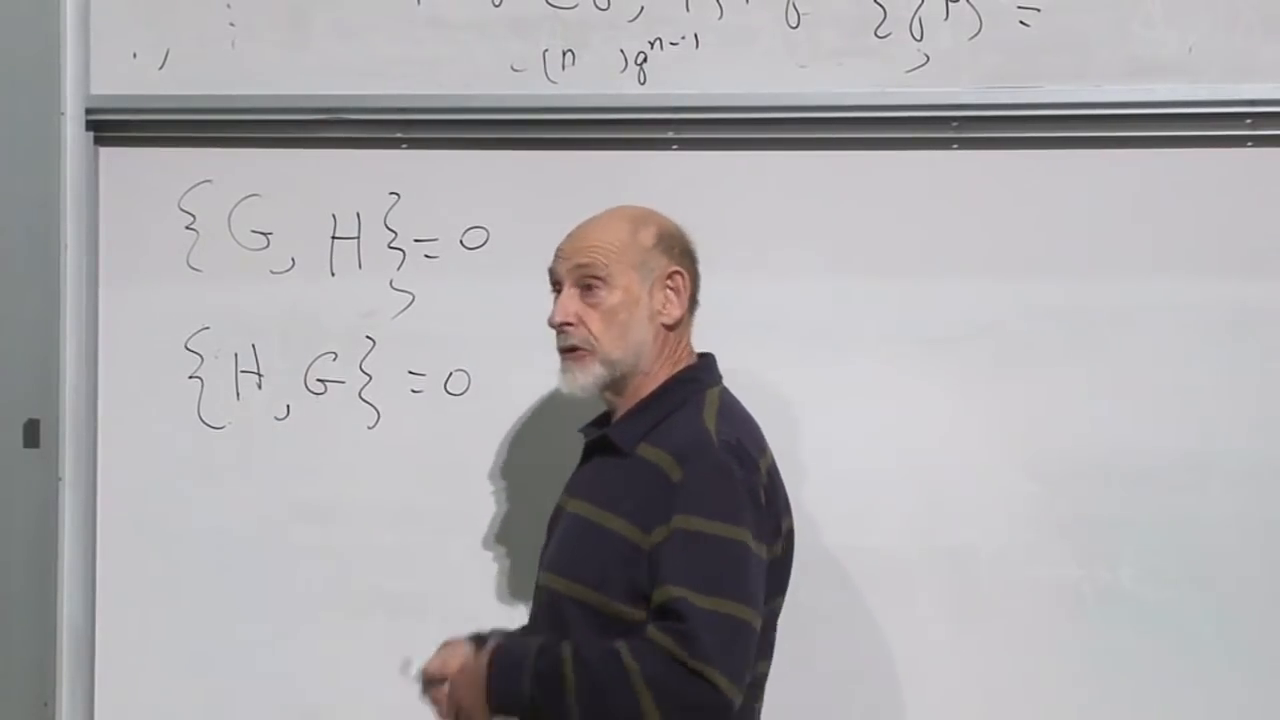
\includegraphics[width=0.82\textwidth]{lecture_08_figure_02.png}
  \caption{Les trois composantes cartésiennes du moment cinétique et leur forme compacte en produit vectoriel.}
  \lectureframe{00:34:00}
\end{figure}

Une rotation autour d’un vecteur unitaire arbitraire \(\boldsymbol n\) est engendrée par
\begin{equation}
  L_{\boldsymbol n}=\boldsymbol n\cdot\boldsymbol L.
  \label{eq:l8-arbitrary-axis}
\end{equation}
Pour un système isolé invariant par rotation, les trois composantes sont conservées. Si seules les rotations autour d’un axe restent des symétries, seule la composante selon cet axe est nécessairement conservée.

\section{Le moment cinétique engendre les rotations}

Au lieu de résoudre tout de suite un problème de dynamique de rotation, examinons ce que \(L_z\) donne sous l’action du crochet. En utilisant
l’équation~\eqref{eq:l8-lz},
\begin{align}
  \{x,L_z\}
  &=\{x,xp_y-yp_x\}
   =-y\{x,p_x\}
   =-y,\\
  \{y,L_z\}
  &=\{y,xp_y-yp_x\}
   =x\{y,p_y\}
   =x,\\
  \{z,L_z\}&=0.
  \label{eq:l8-position-rotation-brackets}
\end{align}
Ce sont exactement les coefficients de l’équation~\eqref{eq:l8-z-rotation}.

\begin{figure}[htbp]
  \centering
  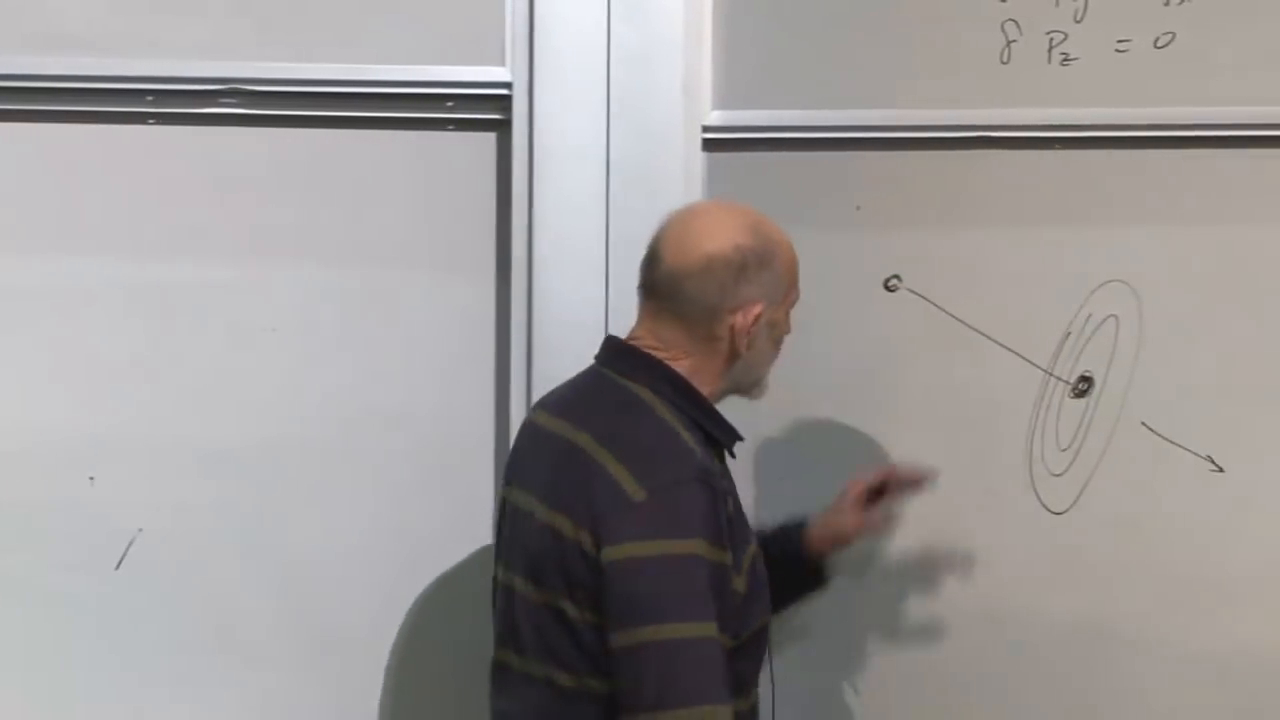
\includegraphics[width=0.82\textwidth]{lecture_08_figure_03.png}
  \caption{Crochets des coordonnées avec \(L_z\) : le crochet reproduit la rotation infinitésimale de \((x,y,z)\).}
  \lectureframe{00:38:41}
\end{figure}

La quantité de mouvement est elle aussi un vecteur, et le même calcul donne
\begin{equation}
  \begin{aligned}
    \{p_x,L_z\}&=-p_y,\\
    \{p_y,L_z\}&=p_x,\\
    \{p_z,L_z\}&=0.
  \end{aligned}
  \label{eq:l8-momentum-rotation-brackets}
\end{equation}

\begin{figure}[htbp]
  \centering
  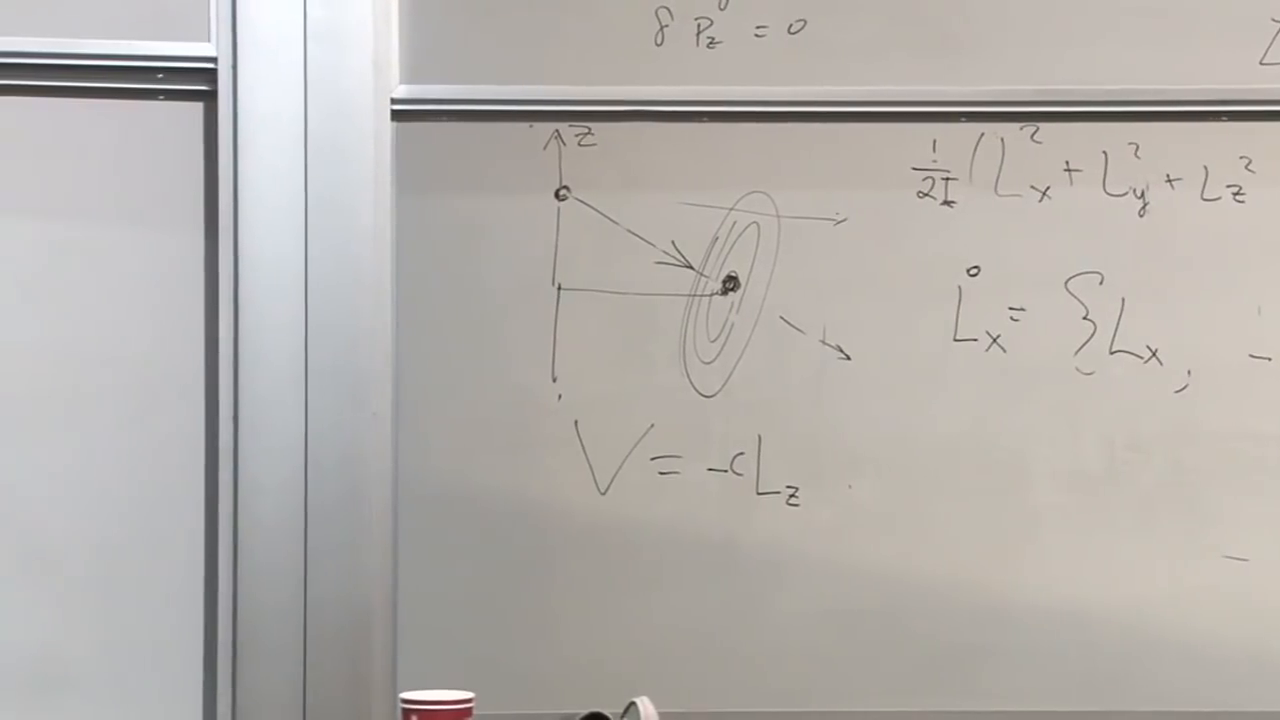
\includegraphics[width=0.82\textwidth]{lecture_08_figure_04.png}
  \caption{La position et la quantité de mouvement suivent le même schéma vectoriel sous la rotation engendrée par \(L_z\).}
  \lectureframe{00:42:08}
\end{figure}

La relation hamiltonienne générale s’écrit donc
\begin{equation}
  \boxed{\delta_G A=\epsilon\{A,G\}.}
  \label{eq:l8-generator-rule}
\end{equation}
Toute fonction de l’espace des phases \(G\) définit une telle transformation canonique infinitésimale. Si \(G=L_z\), c’est une rotation. Si \(G=H\), c’est un petit pas dans le temps.

\begin{classroomqa}
  \audiencequestion{Le cours parle parfois de faire tourner le système et parfois de faire tourner les coordonnées. Quelle convention utilise-t-on dans les équations avec les crochets ? \lecturetimestamp{00:28:22--00:29:35}}
  \lecturerresponse{L’équation~\eqref{eq:l8-z-rotation} fixe la convention : il s’agit de la rotation active infinitésimale
  \((x,y)\mapsto(x-\epsilon y,y+\epsilon x)\). Une rotation passive des axes donne le signe opposé. Une fois la convention fixée, les formules avec les crochets ne présentent aucune ambiguïté.}
\end{classroomqa}

\section{La quantité de mouvement engendre les translations}

Une translation suivant une coordonnée s’écrit
\begin{equation}
  \delta q=\epsilon.
  \label{eq:l8-q-translation}
\end{equation}
Ici, \(F(q)=1\) dans l’équation~\eqref{eq:l8-noether-variation}, donc la quantité conservée correspondante est \(p\). La propriété de générateur prédit
\begin{equation}
  \{f(q),p\}=\frac{df}{dq}.
  \label{eq:l8-translation-derivative}
\end{equation}
Le cours démontre d’abord ce résultat pour les puissances, par récurrence. Le cas de base est
\(\{q,p\}=1\). Supposons que
\begin{equation}
  \{q^{n-1},p\}=(n-1)q^{n-2}.
  \label{eq:l8-induction-hypothesis}
\end{equation}
La règle du produit donne alors
\begin{align}
  \{q^n,p\}
  &=\{q\,q^{n-1},p\}\\
  &=q\{q^{n-1},p\}+\{q,p\}q^{n-1}\\
  &=(n-1)q^{n-1}+q^{n-1}\\
  &=nq^{n-1}.
  \label{eq:l8-power-translation}
\end{align}
La linéarité étend le résultat aux polynômes et aux développements en séries entières convergentes. Plus directement, la définition du crochet donne l’équation~\eqref{eq:l8-translation-derivative} pour toute fonction différentiable \(f(q)\) :
\begin{equation}
  \{f(q),p\}
  =
  \frac{\partial f}{\partial q}
  \frac{\partial p}{\partial p}
  =f'(q).
\end{equation}

\begin{figure}[htbp]
  \centering
  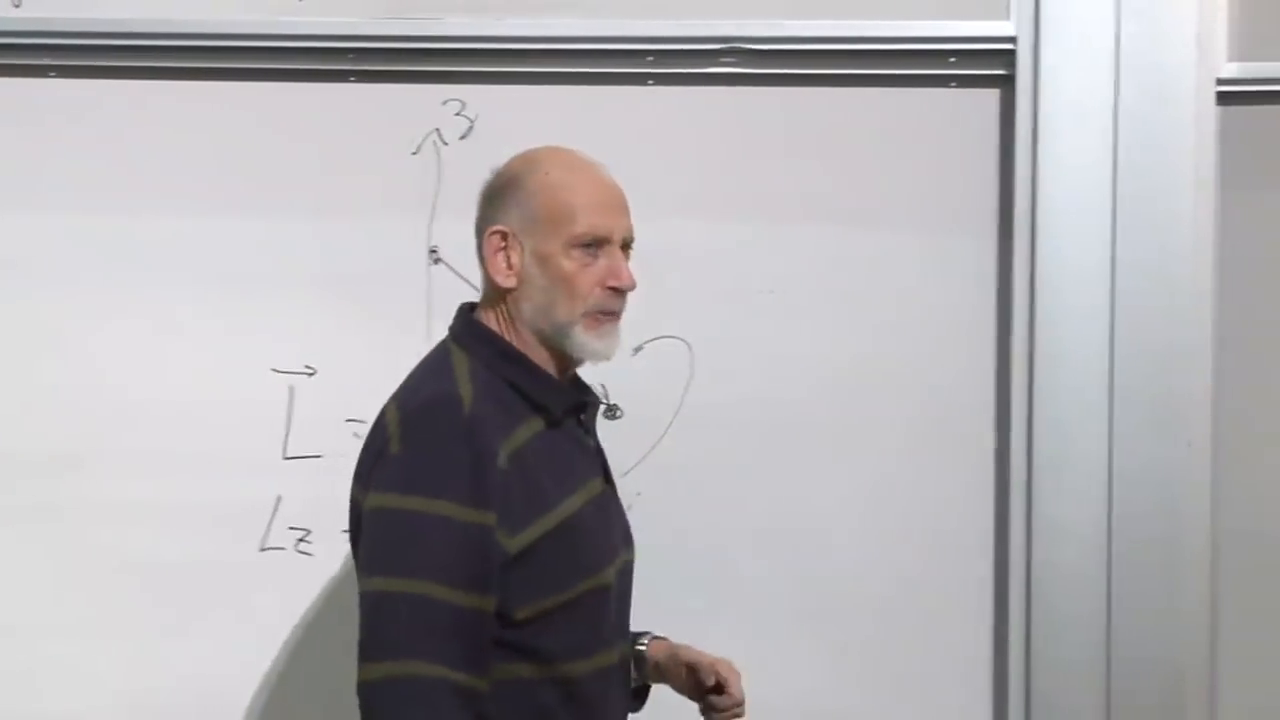
\includegraphics[width=0.82\textwidth]{lecture_08_figure_05.png}
  \caption{Le résultat sur les translations après la démonstration par récurrence : \(\{F(q),p\}=dF/dq\).}
  \lectureframe{00:53:18}
\end{figure}

Nous avons maintenant vu trois manifestations d’une même idée :
\begin{center}
  \begin{tabular}{@{}>{\raggedright\arraybackslash}p{0.37\textwidth}
                      >{\raggedright\arraybackslash}p{0.55\textwidth}@{}}
    \toprule
    Générateur et transformation & Action infinitésimale\\
    \midrule
    \(H\), translation temporelle & \(\delta_tA=\epsilon\{A,H\}\)\\
    \(p_i\), translation spatiale & \(\delta A=\epsilon\{A,p_i\}\)\\
    \(L_i\), rotation & \(\delta A=\epsilon\{A,L_i\}\)\\
    \bottomrule
  \end{tabular}
\end{center}
La quantité conservée associée à une symétrie continue est aussi le générateur de cette symétrie.

\section{Un crochet, deux interprétations}

Soit \(G(q,p)\) un générateur proposé. S’il est conservé et ne dépend pas explicitement du temps, alors
\begin{equation}
  \dot G=\{G,H\}=0.
  \label{eq:l8-g-conserved}
\end{equation}
Par antisymétrie,
\begin{equation}
  \{H,G\}=0.
  \label{eq:l8-h-invariant}
\end{equation}
Les équations sont mathématiquement équivalentes, mais leurs interprétations physiques diffèrent :
\begin{itemize}
  \item \(\{G,H\}=0\) signifie que \(G\) ne varie pas au cours de l’évolution temporelle engendrée par \(H\).
  \item \(\{H,G\}=0\) signifie que \(H\) ne varie pas sous la transformation engendrée par \(G\).
\end{itemize}
La première est une loi de conservation ; la seconde, une symétrie du Hamiltonien. Le lien de Noether se trouve condensé dans un zéro.

\begin{figure}[htbp]
  \centering
  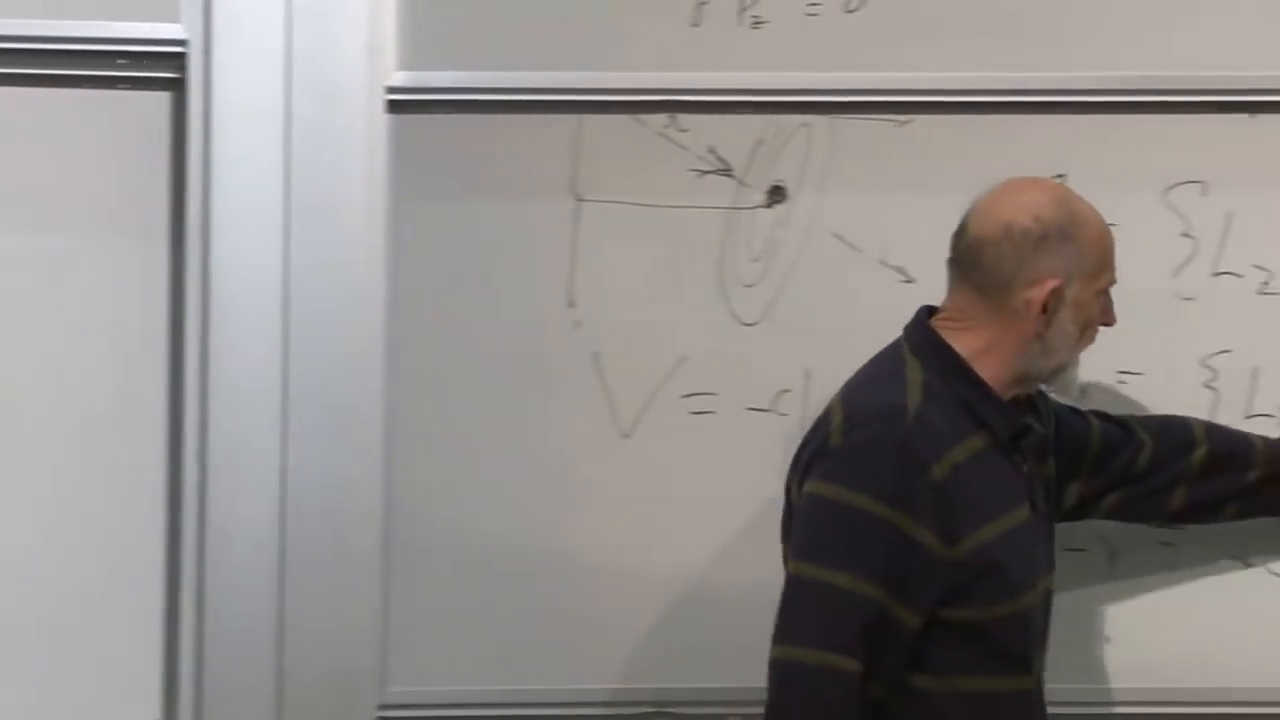
\includegraphics[width=0.82\textwidth]{lecture_08_figure_06.png}
  \caption{Les deux ordres d’un même crochet nul : conservation de \(G\) et invariance de \(H\) sous la transformation engendrée par \(G\).}
  \lectureframe{01:03:05}
\end{figure}

\begin{classroomqa}
  \audiencequestion{Si l’on connaît une quantité conservée, peut-on toujours retrouver la symétrie associée ? \lecturetimestamp{01:01:42--01:02:15}}
  \lecturerresponse{Dans ce cadre hamiltonien, oui : prenons le crochet de chaque variable de l’espace des phases avec \(G\). L’ensemble \(\delta_GA=\epsilon\{A,G\}\) indique comment les variables se transforment. Par exemple, les crochets avec \(L_z\) révèlent une rotation, même si cette interprétation n’était pas connue au départ. Des subtilités globales et liées aux frontières peuvent intervenir dans des cadres plus avancés, mais c’est l’énoncé infinitésimal local qui est utilisé ici.}
\end{classroomqa}

\begin{classroomqa}
  \audiencequestion{Ces équations avec les crochets nous indiquent-elles le mouvement physique à l’origine de la loi de conservation ?
  \lecturetimestamp{00:56:01--00:58:13}}
  \lecturerresponse{Non. Elles identifient la transformation de symétrie, et non la trajectoire réelle. La conservation de \(L_z\) indique une symétrie de rotation ; elle ne signifie pas que la particule décrit un cercle. L’évolution temporelle réelle est engendrée par \(H\). Un crochet avec un autre générateur décrit une autre direction de transformation dans l’espace des phases.}
\end{classroomqa}

\begin{classroomqa}
  \audiencequestion{Existe-t-il un énoncé général sur les transformations qui ne suppose pas déjà la conservation ? \lecturetimestamp{01:02:40--01:04:45}}
  \lecturerresponse{Oui. L’équation~\eqref{eq:l8-generator-rule} définit une transformation infinitésimale pour toute fonction \(G\), qu’elle soit conservée ou non. Elle ne devient une symétrie que lorsque le Hamiltonien est invariant : \(\{H,G\}=0\). Lue dans l’ordre inverse, la même condition indique alors que \(G\) est conservé.}
\end{classroomqa}

\section{L’algèbre du moment cinétique}

Le calcul qui suit nous évite d’entraîner les coordonnées de la particule dans chaque problème de rotation. Commençons par
\[
  L_x=yp_z-zp_y,\qquad
  L_z=xp_y-yp_x.
\]
Dans \(\{L_x,L_z\}\), la plupart des termes croisés s’annulent parce que leurs indices ne forment pas des paires canoniques. Les contractions restantes donnent
\begin{align}
  \{L_x,L_z\}
  &=\{yp_z-zp_y,xp_y-yp_x\}\\
  &=xp_z-zp_x\\
  &=-L_y.
  \label{eq:l8-lx-lz}
\end{align}
Inverser l’ordre supprime le signe moins. La permutation cyclique des coordonnées donne
\begin{equation}
  \boxed{\begin{aligned}
    \{L_x,L_y\}&=L_z,\\
    \{L_y,L_z\}&=L_x,\\
    \{L_z,L_x\}&=L_y.
  \end{aligned}}
  \label{eq:l8-angular-algebra}
\end{equation}
En notation indicielle,
\begin{equation}
  \{L_i,L_j\}=\varepsilon_{ijk}L_k.
  \label{eq:l8-angular-algebra-index}
\end{equation}

\begin{figure}[htbp]
  \centering
  \includegraphics[width=0.82\textwidth]{lecture_08_figure_07.png}
  \caption{L’algèbre cyclique des crochets de Poisson des trois composantes du moment cinétique.}
  \lectureframe{01:10:52}
\end{figure}

On aurait aussi pu prévoir le résultat. Puisque \(\boldsymbol L\) est un vecteur, le crochet de sa composante selon \(x\) avec \(L_z\) doit donner la variation infinitésimale de cette composante sous une rotation autour de \(z\), soit \(-L_y\). Le calcul explicite confirme cet argument géométrique. Ces équations sont aussi les précurseurs classiques des relations de commutation quantiques du moment cinétique.

\section{Un gyroscope à rotation rapide}

À titre d’application, considérons un gyroscope : un volant d’inertie en rotation rapide, dont le centre se trouve à une distance fixe \(R\) d’un pivot. Soit \(\boldsymbol r\) le vecteur allant du pivot au centre du volant. Celui-ci tourne si rapidement autour de son axe que son moment cinétique dominant reste aligné avec cette direction. Dans l’approximation utilisée dans le cours,
\begin{equation}
  \boldsymbol L=\ell\,\boldsymbol r,
  \qquad
  L_z=\ell z,
  \label{eq:l8-L-parallel-r}
\end{equation}
où \(\ell=L/R\) est considéré comme constant. On néglige d’abord les moments cinétiques plus faibles associés à la nutation ou au mouvement de l’axe.

\begin{figure}[htbp]
  \centering
  \begin{tikzpicture}[scale=0.95,>=Latex]
    \coordinate (P) at (0,3.2);
    \coordinate (C) at (3.7,1.55);
    \draw[->] (0,-0.2) -- (0,4.35) node[above] {\(z\)};
    \fill (P) circle (1.7pt) node[left] {pivot};
    \draw[very thick,->] (P) -- (C)
      node[midway,above right] {\(\boldsymbol r\parallel\boldsymbol L\)};
    \fill (C) circle (1.7pt);
    \draw[dashed] (P) -- (0,1.55);
    \draw[dashed] (0,1.55) -- (C);
    \node[left] at (0,1.55) {\(z\)};
    \begin{scope}[shift={(C)},rotate=-24]
      \draw[very thick] (0,0) ellipse (0.65 and 1.35);
      \draw[thick] (0,0) ellipse (0.42 and 0.9);
    \end{scope}
    \draw[->,thick] (2.15,2.85)
      arc[start angle=140,end angle=35,radius=1.65];
  \end{tikzpicture}
  \caption{Approximation du gyroscope à rotation rapide. La distance entre le pivot et le centre est fixe, et le moment cinétique dominant dû à la rotation reste aligné avec l’axe et \(\boldsymbol r\).}
\end{figure}

\begin{figure}[htbp]
  \centering
  \includegraphics[width=0.82\textwidth]{lecture_08_figure_08.png}
  \caption{Schéma au tableau du volant d’inertie, avec \(H_{\rm rot}=L^2/(2I)\), et annulation qui démontre la conservation de \(\boldsymbol L\) en l’absence de couple.}
  \lectureframe{01:18:54}
\end{figure}

\subsection{Sans gravité : pourquoi chaque composante reste constante}

Pour le rotor axialement symétrique simplifié,
\begin{equation}
  H_{\mathrm{rot}}
  =\frac{1}{2I}
  \left(L_x^2+L_y^2+L_z^2\right)
  =\frac{L^2}{2I}.
  \label{eq:l8-rotational-hamiltonian}
\end{equation}
Le coefficient est \(1/(2I)\), et non \(I/2\) ; cette erreur est commise puis corrigée au tableau. En utilisant l’équation~\eqref{eq:l8-angular-algebra},
\begin{align}
  \dot L_x
  &=\{L_x,H_{\mathrm{rot}}\}\\
  &=\frac{1}{2I}\left(
    2L_y\{L_x,L_y\}
    +2L_z\{L_x,L_z\}
  \right)\\
  &=\frac{1}{I}\left(L_yL_z-L_zL_y\right)=0.
  \label{eq:l8-free-lx}
\end{align}
Par permutation cyclique,
\begin{equation}
  \dot L_x=\dot L_y=\dot L_z=0.
  \label{eq:l8-free-angular-momentum}
\end{equation}
Le scalaire \(L^2\) a un crochet nul avec chaque composante \(L_i\) ; dans le langage de cette algèbre, c’est un invariant de Casimir. Ainsi, en l’absence de couple, le gyroscope conserve à la fois la norme et la direction de son moment cinétique.

\begin{classroomqa}
  \audiencequestion{Le moment d’inertie n’est-il qu’un nombre ici ?
  \lecturetimestamp{01:14:23--01:15:05}}
  \lecturerresponse{Pour ce modèle réduit, oui. Il encode la distribution de masse du volant autour de son axe de rotation. Un solide général possède un tenseur d’inertie et un Hamiltonien de rotation
  \(\sum_i L_i^2/(2I_i)\) dans ses axes principaux. Le cours choisit le rotor symétrique à rotation rapide, plus simple, car l’objectif est de présenter la méthode des crochets de Poisson plutôt que de développer la dynamique complète d’un solide.}
\end{classroomqa}

\subsection{Gravité et signe du potentiel}

Prenons la coordonnée verticale \(z\) orientée vers le haut et plaçons le pivot à l’origine. L’énergie potentielle gravitationnelle du centre du volant est
\begin{equation}
  V=Mgz.
  \label{eq:l8-mgz}
\end{equation}
Puisque \(L_z=\ell z\),
\begin{equation}
  V=cL_z,
  \qquad
  c=\frac{Mg}{\ell}=\frac{MgR}{L}.
  \label{eq:l8-potential-lz}
\end{equation}
Ici, \(c>0\) lorsque \(\boldsymbol L\) est choisi parallèle à \(\boldsymbol r\). Si le volant tourne en sens opposé, la relation signée entre \(\boldsymbol L\) et \(\boldsymbol r\) s’inverse, ainsi que la fréquence de précession correspondante avec son signe.

\begin{figure}[htbp]
  \centering
  \includegraphics[width=0.82\textwidth]{lecture_08_figure_09.png}
  \caption{Géométrie à longueur fixe à l’origine de \(\boldsymbol L=\ell\boldsymbol r\) et de \(L_z=\ell z\).}
  \lectureframe{01:25:38}
\end{figure}

\begin{figure}[htbp]
  \centering
  \includegraphics[width=0.82\textwidth]{lecture_08_figure_10.png}
  \caption{Une étape intermédiaire du tableau montre \(V=-cL_z\). Le signe est corrigé plus tard, une fois \(z\) fixé vers le haut : avec \(\boldsymbol L=\ell\boldsymbol r\) et \(\ell>0\), le résultat cohérent est \(V=+cL_z\).}
  \lectureframe{01:22:43}
\end{figure}

\begin{classroomqa}
  \audiencequestion{Pourquoi peut-on remplacer la hauteur par une composante du moment cinétique ? La ligne oblique représente-t-elle un axe ou un vecteur position ?
  \lecturetimestamp{01:22:20--01:25:43}}
  \lecturerresponse{Il vaut mieux désigner la ligne oblique par \(\boldsymbol r\), le vecteur allant du pivot fixe au centre du volant. Un axe physique peut lui être parallèle, mais la relation utilisée dans le calcul est l’approximation de rotation rapide
  \(\boldsymbol L=\ell\boldsymbol r\). Leurs composantes selon \(z\) sont donc proportionnelles. Au fil de la discussion, les étiquettes changent plusieurs fois avant que cette distinction soit établie.}
\end{classroomqa}

\begin{classroomqa}
  \audiencequestion{Quelles hypothèses permettent de considérer \(\ell\) comme constant, et que se passe-t-il si le centre du volant peut glisser radialement ?
  \lecturetimestamp{01:25:43--01:26:38,\allowbreak\ 01:34:22--01:35:00}}
  \lecturerresponse{On suppose que la rotation dominante est beaucoup plus importante que le moment cinétique associé au mouvement lent, et que la distance entre le pivot et le centre est fixe. La norme du moment cinétique de rotation varie alors peu et \(\boldsymbol L\) tourne avec \(\boldsymbol r\). Si le centre pouvait glisser radialement, \(z\) ne serait plus proportionnel à \(L_z\) selon un coefficient constant unique ; le Hamiltonien réduit \(V=cL_z\) ne décrirait donc plus le mouvement.}
\end{classroomqa}

\begin{classroomqa}
  \audiencequestion{Pourquoi le tableau montre-t-il d’abord un signe moins, puis un signe plus ? Le sens de rotation compte-t-il ?
  \lecturetimestamp{01:27:13--01:28:15,\allowbreak\ 01:33:09--01:33:21}}
  \lecturerresponse{Le signe initial résulte d’une erreur faite au tableau et d’une convention d’axe qui n’était pas encore fixée. Une fois \(z\) défini vers le haut, \(V=Mgz\) augmente avec la hauteur. Si \(\boldsymbol L=\ell\boldsymbol r\) avec \(\ell>0\), on obtient \(V=+cL_z\). Inverser le sens de rotation inverse la proportionnalité signée et le sens de la précession, mais ne rétablit pas un choix de signe arbitraire.}
\end{classroomqa}

\subsection{La précession en trois équations courtes}

Le Hamiltonien réduit complet est
\begin{equation}
  H=
  \frac{1}{2I}\left(L_x^2+L_y^2+L_z^2\right)+cL_z.
  \label{eq:l8-full-gyro-hamiltonian}
\end{equation}
Nous avons déjà montré que \(L^2\) a un crochet nul avec chaque \(L_i\). Seul le terme linéaire contribue :
\begin{align}
  \dot L_z&=\{L_z,H\}=0,\\
  \dot L_x&=\{L_x,H\}=c\{L_x,L_z\}=-cL_y,\\
  \dot L_y&=\{L_y,H\}=c\{L_y,L_z\}=cL_x.
  \label{eq:l8-precession-equations}
\end{align}

\begin{figure}[htbp]
  \centering
  \includegraphics[width=0.82\textwidth]{lecture_08_figure_11.png}
  \caption{Les équations finales pour les composantes : \(L_z\) reste constant, tandis que \(L_x\) et \(L_y\) tournent l’un en l’autre.}
  \lectureframe{01:30:35}
\end{figure}

La composante verticale et la norme de la composante horizontale sont constantes :
\begin{equation}
  \frac{d}{dt}(L_x^2+L_y^2)
  =2L_x(-cL_y)+2L_y(cL_x)=0.
\end{equation}
En combinant les composantes horizontales,
\begin{equation}
  L_+=L_x+iL_y,
  \qquad
  \dot L_+=icL_+,
\end{equation}
on obtient
\begin{equation}
  L_+(t)=L_+(0)e^{ict}.
  \label{eq:l8-precession-solution}
\end{equation}
Le vecteur moment cinétique précesse donc autour de l’axe vertical à la vitesse angulaire \(|c|=MgR/L\). Son inclinaison reste constante dans ce mouvement régulier idéalisé.

\begin{classroomqa}
  \audiencequestion{Le terme d’énergie de rotation a-t-il été négligé dans l’écriture des équations de précession ?
  \lecturetimestamp{01:35:01--01:35:49}}
  \lecturerresponse{Non. Il fait partie du Hamiltonien complet, comme dans l’équation~\eqref{eq:l8-full-gyro-hamiltonian}. Il ne contribue tout simplement pas à \(\dot L_i\), car \(\{L_i,L^2\}=0\), annulation déjà démontrée dans le calcul sans couple. La question de l’étudiant explicite cette étape implicite.}
\end{classroomqa}

\begin{classroomqa}
  \audiencequestion{La précession uniforme est-elle un équilibre ? Que se passe-t-il après une petite impulsion ? \lecturetimestamp{01:32:38--01:33:08}}
  \lecturerresponse{Il vaut mieux parler d’un mouvement régulier ou stationnaire que d’un équilibre statique. Une petite impulsion ajoute en général une nutation, c’est-à-dire une oscillation de l’angle d’inclinaison. Pour un volant en rotation très rapide, cette oscillation est faible, ce qui explique pourquoi le traitement réduit ne retient qu’une précession presque uniforme.}
\end{classroomqa}

\begin{classroomqa}
  \audiencequestion{La précession exige-t-elle un support ou un axe réel ?
  \lecturetimestamp{01:31:49--01:32:38,\allowbreak\ 01:33:49--01:35:00}}
  \lecturerresponse{Ce modèle mécanique suppose que la distance entre le pivot et le centre est fixe ; une contrainte doit donc assurer le support. Le résultat algébrique plus général est le suivant : chaque fois qu’un terme du Hamiltonien est linéaire en une composante du moment cinétique, la même algèbre des crochets produit une précession. La source microscopique du moment cinétique n’a pas besoin d’être une véritable roue montée sur un axe.}
\end{classroomqa}

\begin{classroomqa}
  \audiencequestion{Est-ce la même précession que celle du spin de l’électron ou du noyau dans un champ magnétique, ou que celle de l’orbite d’une planète ?
  \lecturetimestamp{01:35:50--01:37:00}}
  \lecturerresponse{Un moment magnétique couplé à un champ magnétique possède un Hamiltonien linéaire en une composante du spin et obéit donc à la même algèbre du moment cinétique. La précession du spin nucléaire est au fondement de la résonance magnétique nucléaire. La précession du périhélie d’une orbite planétaire est un phénomène différent qui partage par hasard le mot \emph{précession} ; le calcul n’est pas le même.}
\end{classroomqa}

\begin{classroomqa}
  \audiencequestion{Le gyroscope monté latéralement est-il essentiellement le même objet qu’une toupie ? \lecturetimestamp{01:37:02--01:37:23}}
  \lecturerresponse{Oui. La distinction relève surtout du vocabulaire géométrique : lorsque l’axe de rotation s’étend latéralement depuis son support, on parle généralement de gyroscope ; lorsqu’il est presque vertical, on parle de toupie. La structure du moment cinétique et du couple est la même.}
\end{classroomqa}

\section{Ce que le calcul a permis d’établir}

Nous n’avons introduit aucun angle d’Euler ni suivi les coordonnées de chaque élément de la roue. Une fois que
\[
  \{L_i,L_j\}=\varepsilon_{ijk}L_k
\]
était connue, les équations des variables qui nous intéressent en ont découlé directement. C’est là la démonstration de puissance visée. L’oscillateur a montré que les crochets de Poisson peuvent reproduire une dynamique familière. Le moment cinétique a montré qu’ils permettent bien davantage :
\begin{itemize}
  \item une quantité conservée engendre la symétrie infinitésimale qui lui est associée ;
  \item la conservation de \(G\) et l’invariance de \(H\) sont les deux interprétations de \(\{G,H\}=0\) ;
  \item l’algèbre des observables peut se refermer sur elle-même, ce qui permet de résoudre la dynamique sans revenir aux coordonnées microscopiques ;
  \item un Hamiltonien linéaire en une composante du moment cinétique produit une précession autour de cet axe.
\end{itemize}
Le cours s’arrête avant les équations d’Euler complètes d’un solide général. Sa conclusion, plus limitée, est déjà complète : les bons générateurs et leur algèbre de Poisson mettent en évidence à la fois la symétrie et le mouvement avec une remarquable économie.

\chapter{Forces magnétiques, potentiels vecteurs et principe de l’action}

\lectureoverview{Les forces électrostatiques suivent le schéma conservatif familier, mais les forces magnétiques dépendent de la vitesse. Pour les intégrer à la mécanique lagrangienne, nous développons d’abord les outils de calcul vectoriel nécessaires, utilisons le caractère sans source du champ magnétique pour introduire un potentiel vecteur, examinons sa liberté de jauge, puis construisons le terme magnétique de l’action.}

\section{Une nouvelle sorte de force}

La discussion précédente du moment cinétique, des gyroscopes et des crochets de Poisson a réuni plusieurs thèmes. En particulier, un corps chargé en rotation dans un champ magnétique précesse à peu près comme un gyroscope. Nous passons maintenant de cette analogie au mouvement d’une particule chargée isolée.

Les forces électrostatiques ne nécessitent aucune nouvelle mécanique. Si \(U(\mathbf x)\) est une énergie potentielle, alors
\begin{equation}
  \mathbf F=-\nabla U(\mathbf x),
\end{equation}
et le raisonnement habituel donne la conservation de la somme des énergies cinétique et potentielle. Pour une particule de charge \(e\) dans un potentiel électrostatique \(V(\mathbf x)\),
\begin{equation}
  U(\mathbf x)=eV(\mathbf x),
  \qquad
  \mathbf F_{\mathrm{el}}=-e\nabla V.
\end{equation}
Les forces magnétiques ont une forme différente. Elles dépendent de la vitesse de la particule et ne peuvent donc pas être introduites simplement en ajoutant une autre énergie potentielle ordinaire. Elles découlent néanmoins d’un principe de l’action et admettent une description lagrangienne comme hamiltonienne. Pour parvenir à cette description, un bref détour essentiel par le calcul vectoriel s’impose.

\section{Champs et opérations locales}

\subsection{Ce qu’un champ représente}

Un champ associe une grandeur physique à chaque point de l’espace et, en général, à chaque instant. La température et la pression sont des champs scalaires. La vitesse du vent est un champ vectoriel. Les champs électrique et magnétique sont des champs vectoriels. D’autres théories comportent des champs scalaires même à l’échelle microscopique, tandis que la gravitation est décrite par un champ tensoriel. Pour la présente discussion, nous omettons toute dépendance temporelle et écrivons les champs comme des fonctions de \(\mathbf x\).

Le caractère local est au cœur de la notion de champ. Imaginons qu’une certaine région soit cachée dans un sac. Pour mesurer le champ électrique dans cette région, plaçons-y une petite charge test et observons son accélération. La force est déterminée par le champ à l’endroit où se trouve la charge, sans qu’il soit nécessaire de consulter séparément toutes les sources lointaines. Le même raisonnement vaut pour un champ magnétique et une charge test en mouvement. Le potentiel vecteur nous obligera plus tard à nuancer cette image simple, mais c’est le bon point de départ.

\subsection{L’opérateur dérivation}

Les dérivées transforment des champs en d’autres champs. Regroupons les trois dérivées spatiales dans
\begin{equation}
  \nabla
  =
  \left(
    \frac{\partial}{\partial x},
    \frac{\partial}{\partial y},
    \frac{\partial}{\partial z}
  \right).
\end{equation}
Ce symbole se lit \emph{del} ou \emph{nabla}. Sa forme de triangle renversé est facile à retenir, mais sa véritable importance tient au fait qu’il se comporte formellement comme un vecteur dont les composantes sont des opérateurs différentiels.

Il s’agit de l’espace physique ordinaire à trois dimensions, et non de l’espace des phases ni d’un espace de configurations à plusieurs particules. De plus, \(\nabla\) n’est pas un champ vectoriel qui puisse exister isolément. Il doit agir sur quelque chose. Si \(T(\mathbf x)\) est un champ scalaire de température, alors
\begin{equation}
  \nabla T
  =
  \left(
    \frac{\partial T}{\partial x},
    \frac{\partial T}{\partial y},
    \frac{\partial T}{\partial z}
  \right)
\end{equation}
est son gradient, qui est un véritable champ vectoriel.

\begin{figure}[htbp]
\centering
\includegraphics[width=0.82\textwidth]{lecture_09_figure_01.png}
\caption{Au tableau, \(\nabla\) est introduit comme vecteur d’opérateurs de dérivation spatiale, puis appliqué à un champ scalaire \(T(\mathbf x)\).}
\lectureframe{00:11:30}
\end{figure}

Un scalaire n’est pas simplement une grandeur écrite avec une seule composante. C’est une grandeur dont la valeur ne dépend pas de l’orientation des axes de coordonnées. La température en est l’exemple classique. Étant donné un champ vectoriel \(\mathbf E\), l’expression locale \(\mathbf E\cdot\mathbf E\) est également un scalaire. En revanche, construire un potentiel par intégration d’un champ est une opération non locale : elle fait intervenir les valeurs le long d’un chemin.

\subsection{Divergence}

Pour un champ vectoriel \(\mathbf A=(A_x,A_y,A_z)\), le scalaire
\begin{equation}
  \nabla\cdot\mathbf A
  =
  \frac{\partial A_x}{\partial x}
  +\frac{\partial A_y}{\partial y}
  +\frac{\partial A_z}{\partial z}
\end{equation}
est sa divergence. En langage des fluides, une divergence positive mesure une tendance locale à s’écouler vers l’extérieur, tandis qu’une divergence négative mesure une tendance à converger vers l’intérieur. Une source de fluide produit une divergence positive ; un puits, une divergence négative. Cette image est qualitative, mais elle rendra manifeste l’absence de sources du champ magnétique.

\section{Produits vectoriels, symboles epsilon et rotationnel}

\subsection{Le produit vectoriel en composantes}

Pour deux vecteurs \(\mathbf V\) et \(\mathbf A\), une composante de leur produit vectoriel est
\begin{equation}
  (\mathbf V\times\mathbf A)_x
  =
  V_yA_z-V_zA_y.
\end{equation}
Les deux autres s’obtiennent par permutation cyclique de \(x\to y\to z\to x\). Il est utile de remplacer \(x,y,z\) par les indices \(1,2,3\). Le symbole de Kronecker est défini par
\begin{equation}
  \delta_{ij}
  =
  \begin{cases}
    1,&i=j,\\
    0,&i\ne j,
  \end{cases}
\end{equation}
et le symbole de Levi--Civita par
\begin{equation}
  \epsilon_{123}=\epsilon_{231}=\epsilon_{312}=1,
  \qquad
  \epsilon_{132}=\epsilon_{321}=\epsilon_{213}=-1,
\end{equation}
avec \(\epsilon_{ijk}=0\) dès que deux indices quelconques coïncident. Un ordre cyclique autour d’une horloge à trois heures donne les signes positifs ; l’ordre inverse donne les signes négatifs. L’échange de deux indices quelconques inverse le signe : \(\epsilon_{ijk}\) est donc complètement antisymétrique.

Nous utilisons aussi la convention de sommation : tout indice répété dans un terme est sommé de \(1\) à \(3\). Les trois équations du produit vectoriel s’écrivent alors
\begin{equation}
  (\mathbf V\times\mathbf A)_i
  =
  \epsilon_{ijk}V_jA_k.
\end{equation}
Par exemple, en posant \(i=1\), seuls \((j,k)=(2,3)\) et \((3,2)\) subsistent :
\begin{equation}
  (\mathbf V\times\mathbf A)_1
  =
  \epsilon_{123}V_2A_3
  +\epsilon_{132}V_3A_2
  =
  V_2A_3-V_3A_2.
\end{equation}
Cette notation compacte contient donc exactement la règle usuelle de calcul des composantes.

\subsection{Un vecteur déguisé en matrice antisymétrique}

Il existe une deuxième représentation :
\begin{equation}
  V_iA_j-V_jA_i
  =
  \epsilon_{ijk}(\mathbf V\times\mathbf A)_k.
\end{equation}
Le membre de gauche porte deux indices et est antisymétrique sous \(i\leftrightarrow j\). Sa représentation matricielle a la forme
\begin{equation}
  M_{ij}
  =
  \begin{pmatrix}
    0&M_{12}&M_{13}\\
    -M_{12}&0&M_{23}\\
    -M_{13}&-M_{23}&0
  \end{pmatrix}.
\end{equation}
Les éléments diagonaux sont nuls, et le triangle inférieur est déterminé par le triangle supérieur. Il y a donc trois composantes indépendantes.

\begin{figure}[htbp]
\centering
\includegraphics[width=0.82\textwidth]{lecture_09_figure_02.png}
\caption{Une composante du produit vectoriel et le tableau antisymétrique schématique \(3\times3\), qui sert à dénombrer ses éléments indépendants. Les marques dans les cases sont des moyens mnémotechniques, pas des symboles supplémentaires.}
\lectureframe{00:34:20}
\end{figure}

\begin{classroomqa}
\audiencequestion{Le produit vectoriel, ou son identification à un autre vecteur, a-t-il un sens au-delà de trois dimensions ?}
\lecturerresponse{L’objet antisymétrique à deux indices a un sens en toute dimension, mais son identification à un vecteur est propre à trois dimensions. Un vecteur tridimensionnel a trois composantes, et une matrice antisymétrique \(3\times3\) a trois composantes indépendantes. En quatre dimensions, les nombres correspondants sont quatre et six, puisque \(4(4-1)/2=6\). L’objet antisymétrique existe toujours et s’interprète naturellement comme une 2-forme, mais ce n’est pas un autre vecteur à quatre composantes.}
\end{classroomqa}

\subsection{Rotationnel}

En remplaçant \(\mathbf V\) par \(\nabla\), on définit le rotationnel :
\begin{equation}
  (\nabla\times\mathbf A)_i
  =
  \epsilon_{ijk}\frac{\partial A_k}{\partial x_j}.
\end{equation}
Dans les composantes usuelles,
\begin{align}
  (\nabla\times\mathbf A)_x
  &=
  \frac{\partial A_z}{\partial y}
  -\frac{\partial A_y}{\partial z},\\
  (\nabla\times\mathbf A)_y
  &=
  \frac{\partial A_x}{\partial z}
  -\frac{\partial A_z}{\partial x},\\
  (\nabla\times\mathbf A)_z
  &=
  \frac{\partial A_y}{\partial x}
  -\frac{\partial A_x}{\partial y}.
\end{align}
La divergence mesure la dispersion locale, tandis que le rotationnel mesure la circulation locale. Un fluide en rotation autour d’un axe a un rotationnel non nul suivant cet axe. L’image est particulièrement parlante pour les champs de vitesse, bien que la définition s’applique à tout champ vectoriel.

\section{Deux identités structurelles}

Deux propriétés fourniront presque tout le travail mathématique :
\begin{equation}
  \nabla\cdot(\nabla\times\mathbf A)=0,
  \qquad
  \nabla\times(\nabla s)=0.
\end{equation}
La première découle du fait que les dérivées secondes sont symétriques, alors que \(\epsilon_{ijk}\) est antisymétrique :
\begin{equation}
  \nabla\cdot(\nabla\times\mathbf A)
  =
  \epsilon_{ijk}\partial_i\partial_j A_k
  =0.
\end{equation}
La seconde découle de l’égalité des dérivées partielles mixtes :
\begin{equation}
  \bigl[\nabla\times(\nabla s)\bigr]_i
  =
  \epsilon_{ijk}\partial_j\partial_k s
  =0.
\end{equation}

\begin{figure}[htbp]
\centering
\includegraphics[width=0.80\textwidth]{lecture_09_figure_03.png}
\caption{Première identité au tableau : la divergence de tout rotationnel est nulle.}
\lectureframe{00:38:26}
\end{figure}

Ce sont les implications faciles, qui se prêtent bien au devoir ou au petit quiz annoncé pour le cours. Les réciproques demandent davantage de précautions. Localement, ou globalement sur un domaine convenablement simplement connexe ou contractile,
\begin{align}
  \nabla\cdot\mathbf F=0
  &\quad\Longrightarrow\quad
  \mathbf F=\nabla\times\mathbf A,\\
  \nabla\times\mathbf F=0
  &\quad\Longrightarrow\quad
  \mathbf F=\nabla s.
\end{align}
Sans cette précision sur le domaine, des trous et d’autres propriétés topologiques globales peuvent faire obstacle à ces conclusions. Le cours utilise la forme locale, qui est exactement celle dont nous avons besoin par la suite.

\section{Pourquoi le champ magnétique est un rotationnel}

\subsection{Absence de sources magnétiques observées}

Un champ magnétique \(\mathbf B\) est défini opérationnellement par son effet sur les particules chargées et les courants. En électromagnétisme ordinaire, en l’absence de monopôles magnétiques,
\begin{equation}
  \nabla\cdot\mathbf B=0.
\end{equation}
Cela diffère du champ électrique, dont la divergence est proportionnelle à la densité de charge électrique. Les charges électriques sont des sources et des puits du flux électrique. Aucune source ni aucun puits isolé de flux magnétique n’a été observé.

La présence de monopôles magnétiques modifierait cette équation. Les théories unifiées des champs donnent souvent des raisons théoriques de s’attendre à l’existence de tels objets ; s’ils existent, ils sont peut-être trop massifs pour être produits dans les expériences actuellement possibles. La théorie présentée ici suppose donc une densité de charge magnétique nulle.

\begin{classroomqa}
\audiencequestion{Qu’est-ce qu’un monopôle magnétique ? Les aimants ordinaires ont déjà un pôle nord et un pôle sud.}
\lecturerresponse{Un monopôle isolé serait une véritable source ou un véritable puits de champ magnétique, analogue à une charge électrique. Un aimant droit ordinaire est différent. Les lignes de champ qui émergent près de son pôle nord se courbent dans l’espace et reviennent par le pôle sud, puis se poursuivent à l’intérieur de l’aimant. Ce qui ressemble à l’extérieur à une source et à un puits est relié, comme un fluide qui circule dans une canalisation cachée. Il n’y a aucune création ni destruction nette de flux magnétique.}
\end{classroomqa}

\begin{figure}[htbp]
\centering
\includegraphics[width=0.76\textwidth]{lecture_09_figure_04.png}
\caption{Le tableau oppose les sources apparentes nord et sud, tout en reliant leurs lignes de champ à travers l’aimant, pour souligner que le flux magnétique n’y commence ni ne s’y termine.}
\lectureframe{00:44:56}
\end{figure}

Puisque \(\mathbf B\) est de divergence nulle, le théorème réciproque permet d’écrire, au moins localement,
\begin{equation}
  \boxed{\mathbf B=\nabla\times\mathbf A}.
\end{equation}
Le champ \(\mathbf A\) est le potentiel vecteur. À première vue, il peut sembler inutile de redécrire ainsi le champ mesurable \(\mathbf B\). Son utilité ne deviendra claire que lorsque nous construirons l’action.

\subsection{Le potentiel vecteur n’est pas unique}

Si \(\mathbf A\) est un potentiel vecteur, alors
\begin{equation}
  \mathbf A'=\mathbf A+\nabla s
\end{equation}
en est un autre, car
\begin{equation}
  \nabla\times\mathbf A'
  =
  \nabla\times\mathbf A+\nabla\times(\nabla s)
  =
  \mathbf B.
\end{equation}
Cette transformation est une \emph{transformation de jauge}. Le champ magnétique est invariant de jauge.

\begin{figure}[htbp]
\centering
\includegraphics[width=0.80\textwidth]{lecture_09_figure_05.png}
\caption{La relation de définition \(\mathbf B=\nabla\times\mathbf A\) et le décalage de jauge \(\mathbf A'=\mathbf A+\nabla s\) figurent ensemble au tableau.}
\lectureframe{01:03:01}
\end{figure}

La prononciation est \emph{gauge}, et non \emph{gouache} ni \emph{gouge}--, distinction que le cours impose avec une sévérité feinte. Le mot est d’origine historique. Il est apparu lors d’une première tentative pour relier cette liberté à la comparaison d’étalons de longueur en différents lieux ; cette interprétation initiale n’a pas résisté, mais le nom est resté.

\begin{classroomqa}
\audiencequestion{Dans cette discussion, une transformation de jauge désigne-t-elle précisément \(\mathbf A\mapsto\mathbf A+\nabla s\) ?}
\lecturerresponse{Oui. C’est la transformation électromagnétique complète considérée ici. Les transformations de jauge en théorie de Yang--Mills et dans d’autres théories des champs généralisent la même idée, mais l’électromagnétisme ne nécessite que l’ajout du gradient d’un scalaire.}
\end{classroomqa}

La non-unicité précise aussi ce qui est directement mesurable. Dans une petite région, une particule chargée réagit au \(\mathbf B\) local, et tous les potentiels vecteurs reliés par une transformation de jauge prédisent la même force en ce lieu. Aucune expérience locale de ce type classique ne permet d’attribuer une valeur unique à \(\mathbf A\).

\begin{classroomqa}
\audiencequestion{L’ajout d’un gradient décrit-il entièrement la non-unicité ?}
\lecturerresponse{Localement, sur un domaine simple, oui. Si \(\nabla\times\mathbf A'=\nabla\times\mathbf A\), alors \(\nabla\times(\mathbf A'-\mathbf A)=0\), et la différence est donc un gradient. Globalement, un domaine multiplement connexe peut présenter des subtilités supplémentaires. L’ajout d’un vecteur constant est déjà inclus, puisqu’un vecteur constant est le gradient d’une fonction scalaire linéaire. Ajouter une constante à \(s\) ne change rien, car son gradient s’annule.}
\end{classroomqa}

\begin{classroomqa}
\audiencequestion{Si la liberté de jauge a une raison physique profonde, quelle est-elle ?}
\lecturerresponse{Le cours remet à plus tard cette interprétation plus profonde. La première étape utile consiste à exploiter cette liberté et à voir comment elle intervient dans l’action. Une fois le formalisme familier, il devient plus facile de comprendre pourquoi les descriptions de jauge sont indispensables.}
\end{classroomqa}

\section{Un champ magnétique, plusieurs potentiels}

Considérons l’exemple le plus simple possible,
\begin{equation}
  \mathbf B=b\,\hat{\mathbf z},
  \qquad
  B_x=B_y=0,
  \qquad
  B_z=b,
\end{equation}
où \(b\) est constant. Un potentiel vecteur possible est
\begin{equation}
  \mathbf A^{(1)}=(0,bx,0).
\end{equation}
En effet,
\begin{equation}
  (\nabla\times\mathbf A^{(1)})_z
  =
  \frac{\partial A_y^{(1)}}{\partial x}
  -\frac{\partial A_x^{(1)}}{\partial y}
  =b,
\end{equation}
et les autres composantes du rotationnel s’annulent.

Ce choix semble privilégier la direction \(y\), alors que le champ physique est invariant par rotation dans le plan \(x\)-\(y\). Un deuxième choix rend l’arbitraire manifeste :
\begin{equation}
  \mathbf A^{(2)}=(-by,0,0).
\end{equation}
Il donne
\begin{equation}
  (\nabla\times\mathbf A^{(2)})_z
  =
  0-\frac{\partial(-by)}{\partial y}
  =b.
\end{equation}
La différence entre les deux potentiels est
\begin{equation}
  \mathbf A^{(2)}-\mathbf A^{(1)}
  =
  (-by,-bx,0)
  =
  \nabla(-bxy).
\end{equation}
Ils sont donc équivalents de jauge. Le choix invariant par rotation,
\begin{equation}
  \mathbf A^{(\mathrm{sym})}
  =
  \frac12\,\mathbf B\times\mathbf r
  =
  \left(-\frac{by}{2},\frac{bx}{2},0\right),
\end{equation}
est un autre élément de la même famille.

\begin{figure}[htbp]
\centering
\includegraphics[width=0.80\textwidth]{lecture_09_figure_06.png}
\caption{Deux parties du tableau présentent les choix \(A_y=bx\) et \(A_x=-by\), qui produisent tous deux le même champ uniforme \(B_z=b\).}
\lectureframe{01:07:20}
\end{figure}

\begin{classroomqa}
\audiencequestion{Est-ce la même ambiguïté que celle qui consiste à disposer différemment les bobines parcourues par un courant pour produire un champ ?}
\lecturerresponse{Non. Des dispositions différentes des courants sont des sources physiques différentes et peuvent produire des champs différents ailleurs, même si elles donnent le même champ dans une région. La liberté de jauge subsiste même après que le champ magnétique a été spécifié partout : un même \(\mathbf B\) physique admet encore de nombreux potentiels vecteurs.}
\end{classroomqa}

\begin{classroomqa}
\audiencequestion{Peut-on se représenter l’ajout d’un gradient comme un étirement ou une compression sans torsion supplémentaire ?}
\lecturerresponse{C’est une intuition géométrique utile. Le rotationnel détecte la composante de torsion locale, et un gradient pur a un rotationnel nul. Cette propriété s’exprime exactement par \(\nabla\times\nabla s=0\).}
\end{classroomqa}

\begin{classroomqa}
\audiencequestion{Existe-t-il une relation fixe entre la direction de \(\mathbf A\) et celle de \(\mathbf B\) ?}
\lecturerresponse{Il n’existe aucune relation indépendante de la jauge. Dans les exemples ci-dessus, on a \(A_z=0\), mais on pourrait ajouter une constante \(A_z\) sans modifier aucune dérivée. Alors \(\mathbf A\) ne serait plus perpendiculaire à \(\mathbf B\). Dans cette discussion classique, seul le rotationnel possède un contenu physique invariant.}
\end{classroomqa}

Il existe un analogue plus limité en électrostatique. Puisque \(\mathbf E=-\nabla V\), remplacer \(V\) par \(V+C\) ne modifie pas \(\mathbf E\). Le terme \emph{potentiel vecteur} a été choisi en partie par analogie avec cette liberté du potentiel scalaire ordinaire : on peut modifier le potentiel d’une manière qui laisse le champ physique inchangé.

\section{La force de Lorentz}

Nous pouvons maintenant énoncer la loi de force que le principe de l’action doit reproduire. Avec les conventions utilisées ici,
\begin{equation}
  \boxed{
  \mathbf F
  =
  e\left(
    \mathbf E+\frac{\mathbf v}{c}\times\mathbf B
  \right)
  =
  -e\nabla V+\frac{e}{c}\mathbf v\times\mathbf B
  }.
\end{equation}
Le symbole \(e\) désigne la charge électrique de la particule, \(\mathbf v=\dot{\mathbf x}\) sa vitesse et \(V\) le potentiel scalaire. La notation ne doit pas nous inciter à confondre \(V\) et \(\mathbf v\). En unités SI, \(V\) se mesure en volts et \(e\) en coulombs ; le facteur \(1/c\) affiché relève du système d’unités utilisé dans le cours. Le point structurel est indépendant des unités.

\begin{figure}[htbp]
\centering
\includegraphics[width=0.82\textwidth]{lecture_09_figure_07.png}
\caption{Les contributions électrique et magnétique à la force de Lorentz sont présentées ensemble. La contribution magnétique est proportionnelle à \(\mathbf v\times\mathbf B\).}
\lectureframe{00:58:54}
\end{figure}

Le terme électrique est conservatif et déjà familier. Le terme magnétique est nouveau. Il s’annule pour une particule immobile et est perpendiculaire à \(\mathbf v\) comme à \(\mathbf B\). Par conséquent,
\begin{equation}
  \mathbf v\cdot\mathbf F_{\mathrm{mag}}
  =
  \frac{e}{c}\mathbf v\cdot(\mathbf v\times\mathbf B)
  =0.
\end{equation}
Un champ magnétique statique dévie la trajectoire, mais n’effectue aucun travail sur la particule. Il en va autrement du frottement visqueux, qui est dirigé à l’opposé de la vitesse et dissipe l’énergie cinétique.

Le facteur \(v/c\) indique aussi pourquoi, pour des échelles de champ comparables dans ces conventions, les effets magnétiques sont souvent plus faibles que les effets électriques lorsque les particules se déplacent lentement. Les électrons étant suffisamment légers pour atteindre de grandes vitesses, leur déviation magnétique reste facile à observer.

Historiquement, les forces exercées sur les fils parcourus par un courant ont été connues avant que la force sur une charge isolée soit mise en évidence. Lorentz a compris que la force sur le fil pouvait s’expliquer en attribuant le terme dépendant de la vitesse à chaque charge en mouvement. L’expression complète, qui réunit les contributions électrique et magnétique, est aujourd’hui appelée loi de force de Lorentz, bien que, dans la présente discussion, la partie nouvelle soit la contribution magnétique.

\begin{classroomqa}
\audiencequestion{L’expression complète a-t-elle un symbole particulier, ou seule la contribution magnétique est-elle la force de Lorentz ?}
\lecturerresponse{L’expression complète est simplement la force \(\mathbf F=m\mathbf a\), couramment appelée force de Lorentz. Le terme magnétique est celui qui, historiquement, est le plus directement associé à Lorentz. Les champs électrique et magnétique sont profondément liés par la relativité, mais cette unification n’est pas nécessaire pour le problème de mécanique qui nous occupe.}
\end{classroomqa}

\subsection{L’analogie avec la force de Coriolis}

Nous avons déjà rencontré le produit vectoriel d’une vitesse par un vecteur fixe. Dans un référentiel en rotation de vitesse angulaire \(\boldsymbol\omega\), la force de Coriolis s’écrit
\begin{equation}
  \mathbf F_{\mathrm{Cor}}
  =
  2m\,\mathbf v\times\boldsymbol\omega.
\end{equation}
Elle a la même forme algébrique que la force magnétique :
\begin{equation}
  2m\boldsymbol\omega
  \quad\longleftrightarrow\quad
  \frac{e}{c}\mathbf B.
\end{equation}
Un champ magnétique uniforme perpendiculaire à un plan dévie donc les trajectoires des particules chargées d’une manière très semblable à celle dont un référentiel en rotation dévie les corps en mouvement.

\begin{figure}[htbp]
\centering
\includegraphics[width=0.82\textwidth]{lecture_09_figure_08.png}
\caption{La force de Lorentz reste à gauche, tandis que le tableau lui associe la forme correspondante de la force de Coriolis \(2m\,\mathbf v\times\boldsymbol\omega\).}
\lectureframe{01:02:08}
\end{figure}

\begin{classroomqa}
\audiencequestion{La force de Coriolis est dite fictive. Est-elle moins réelle que la force magnétique parce qu’elle dépend de la vitesse ?}
\lecturerresponse{La dépendance à la vitesse n’est pas en cause. Une personne sur une plateforme en rotation peut tenir un objet en mouvement et ressentir la force de Coriolis. On la dit fictive parce qu’elle disparaît dans un référentiel inertiel, tandis que le référentiel en rotation est précisément défini par la présence de tels termes d’inertie. Le mot \emph{réel} est souvent moins utile qu’une indication du référentiel et de l’équation utilisés.}
\end{classroomqa}

On peut pousser l’analogie au moyen d’une petite expérience de pensée. Sur une plateforme en rotation, un champ électrostatique convenable peut compenser le terme centrifuge pour une particule donnée, tandis qu’un champ magnétique uniforme convenable peut compenser la force de Coriolis. Cette compensation ne fonctionne que pour un rapport charge/masse donné : les forces électrique et magnétique sont proportionnelles à \(e\), tandis que les forces d’inertie sont proportionnelles à \(m\). Une configuration de champ réglée pour les électrons ne compenserait pas les mêmes termes pour des particules ayant un rapport \(e/m\) différent.

\section{Construire l’action d’une particule chargée}

\subsection{Action stationnaire à extrémités fixes}

Nous posons maintenant la question centrale : peut-on déduire la force de Lorentz d’un principe de l’action ? Oui, mais le potentiel vecteur est indispensable. Un lagrangien construit localement à partir de la particule et de \(\mathbf B\) seuls ne produit pas la force magnétique requise. Plutôt que de démontrer cette impossibilité, construisons directement l’action qui convient.

Pour une trajectoire \(\mathbf x(t)\), écrivons
\begin{equation}
  S[\mathbf x]
  =
  \int_{t_i}^{t_f}L(\mathbf x,\dot{\mathbf x},t)\,dt.
\end{equation}
Le cours utilise la même lettre manuscrite pour l’action et le potentiel vecteur ; nous noterons l’action \(S\) et le potentiel vecteur \(\mathbf A\). Le chemin physique rend \(S\) stationnaire sous les variations qui maintiennent fixes ses deux extrémités. L’expression traditionnelle \emph{action minimale} est commode, bien que « action stationnaire » soit plus exact, car l’extremum n’est pas nécessairement un minimum.

Le fait que les extrémités soient fixes est important. On peut imaginer que les bouts de la trajectoire sont cloués au tableau tandis que l’intérieur oscille. Il s’agit d’une trajectoire de mécanique ordinaire, et non d’un objet de théorie des cordes ; l’image de la corde sert uniquement à visualiser la variation.

\subsection{Quels termes peuvent figurer dans le lagrangien ?}

Lorsque tous les champs sont nuls, le lagrangien est l’énergie cinétique,
\begin{equation}
  L_0=\frac{m}{2}\dot{\mathbf x}^{\,2}.
\end{equation}
Le terme électrostatique est également classique :
\begin{equation}
  L_{\mathrm{el}}=-eV(\mathbf x).
\end{equation}
Plusieurs indices doivent guider le choix du terme magnétique :
\begin{enumerate}
  \item il doit être proportionnel à la charge \(e\) ;
  \item il doit contenir le facteur \(1/c\) dans les unités du cours ;
  \item il doit faire intervenir la vitesse ;
  \item il doit être un scalaire par rotation.
\end{enumerate}

L’essai tentant \(\mathbf B\cdot\dot{\mathbf x}\) est un scalaire et contient une vitesse, mais il donne une équation du mouvement erronée. Le terme correct fait intervenir le potentiel vecteur :
\begin{equation}
  L_{\mathrm{mag}}
  =
  \frac{e}{c}\mathbf A(\mathbf x)\cdot\dot{\mathbf x}
  =
  \frac{e}{c}A_i(\mathbf x)\dot x_i.
\end{equation}
Le lagrangien électromagnétique complet, indépendant du temps, est donc
\begin{equation}
  \boxed{
  L
  =
  \frac{m}{2}\dot{\mathbf x}^{\,2}
  +\frac{e}{c}\mathbf A(\mathbf x)\cdot\dot{\mathbf x}
  -eV(\mathbf x)
  }.
\end{equation}
Le cours 10 appliquera les équations d’Euler--Lagrange et montrera explicitement que cette expression produit la force de Lorentz.

\begin{figure}[htbp]
\centering
\includegraphics[width=0.82\textwidth]{lecture_09_figure_09.png}
\caption{Le lagrangien est achevé au tableau : un terme cinétique libre auquel s’ajoute \((e/c)A_i\dot x_i\).}
\lectureframe{01:26:36}
\end{figure}

\section{Les transformations de jauge ne modifient que les extrémités}

La contribution magnétique à l’action est
\begin{equation}
  S_{\mathrm{mag}}
  =
  \frac{e}{c}
  \int_{t_i}^{t_f}A_i(\mathbf x)\dot x_i\,dt.
\end{equation}
Puisque \(\dot x_i\,dt=dx_i\), il s’agit d’une intégrale curviligne le long du chemin de la particule \(\gamma\) :
\begin{equation}
  S_{\mathrm{mag}}
  =
  \frac{e}{c}\int_\gamma A_i\,dx_i
  =
  \frac{e}{c}\int_\gamma\mathbf A\cdot d\mathbf x.
\end{equation}
Découpons le chemin en petits segments, prenons la composante de \(\mathbf A\) suivant chaque segment, multiplions-la par la longueur de celui-ci et additionnons les résultats. Telle est la signification géométrique de l’intégrale.

Effectuons maintenant la transformation de jauge
\begin{equation}
  A_i\longmapsto A_i+\partial_i s.
\end{equation}
L’action varie de
\begin{align}
  \Delta S
  &=
  \frac{e}{c}\int_\gamma \partial_i s\,dx_i\\
  &=
  \frac{e}{c}\int_\gamma ds\\
  &=
  \frac{e}{c}
  \left[
    s(\mathbf x_f)-s(\mathbf x_i)
  \right].
\end{align}
Chaque segment infinitésimal contribue par la valeur de \(s\) à une extrémité moins sa valeur à l’autre. En faisant la somme, toutes les contributions intérieures s’annulent en cascade, ne laissant que les deux extrémités.

\begin{figure}[htbp]
\centering
\includegraphics[width=0.82\textwidth]{lecture_09_figure_10.png}
\caption{L’intégrale curviligne, sa décomposition en petits segments du chemin et le résultat aux extrémités \(s(\mathbf x_f)-s(\mathbf x_i)\).}
\lectureframe{01:32:31}
\end{figure}

\begin{classroomqa}
\audiencequestion{Si l’action varie sous une transformation de jauge, pourquoi la trajectoire ne change-t-elle pas ?}
\lecturerresponse{Le principe de l’action compare des chemins ayant les mêmes points initial et final. La quantité ajoutée ne dépend que de ces extrémités ; elle a donc la même valeur pour tous les chemins comparés. Sa variation est nulle. La valeur numérique de l’action n’est pas strictement invariante, mais les équations d’Euler--Lagrange et la trajectoire physique sont invariantes de jauge.}
\end{classroomqa}

Cette distinction constitue le principal résultat conceptuel du cours :
\begin{equation}
  \begin{aligned}
    S&\ \hbox{may shift by an endpoint term},\\
    \delta S&\ \hbox{and the equations of motion do not}.
  \end{aligned}
\end{equation}
La liberté de jauge est donc compatible avec le principe de l’action. Le potentiel vecteur peut figurer dans le lagrangien même si le champ magnétique ne sélectionne aucun \(\mathbf A\) de manière unique.

\section{La suite du raisonnement}

Le présent cours a réuni les outils et construit l’action, mais s’arrête délibérément avant de faire varier cette action. Les étapes suivantes sont maintenant fixées :
\begin{enumerate}
  \item appliquer les équations d’Euler--Lagrange et retrouver
  \(\mathbf F_{\mathrm{mag}}=(e/c)\mathbf v\times\mathbf B\);
  \item calculer la quantité de mouvement canonique, qui différera de \(m\mathbf v\);
  \item construire le hamiltonien ;
  \item identifier les lois de conservation ;
  \item résoudre le mouvement d’une particule chargée dans un champ magnétique uniforme.
\end{enumerate}

Le chemin qui mène à ces résultats explique pourquoi le potentiel vecteur a été introduit. Le champ magnétique est le rotationnel mesurable localement, mais le potentiel vecteur est l’objet qui se couple naturellement au chemin d’une particule. Les transformations de jauge ne modifient ce couplage qu’aux extrémités fixes, laissant la mécanique inchangée.
\chapter{Invariance de jauge et mouvement des particules chargées}

\lectureoverview{Le champ magnétique est à divergence nulle ; il peut donc être représenté par un potentiel vecteur. Cette représentation n’est pas unique, mais c’est précisément ce qui permet d’introduire les forces magnétiques dans le principe de moindre action. Nous déduisons la force de Lorentz, distinguons la quantité de mouvement canonique de la quantité de mouvement mécanique, construisons le Hamiltonien et utilisons deux jauges différentes pour résoudre le mouvement dans un champ magnétique uniforme. Pour conclure, nous situons cette mécanique particulaire dans les domaines plus vastes de la théorie de Maxwell, des monopôles magnétiques et de la dynamique dans l’espace des phases.}

\section{Dernière étape du cours de mécanique}

Le cours commence par une petite surprise dans le calendrier. Le programme consiste à terminer l’étude des particules chargées dans des champs magnétiques, peut-être à ajouter les champs électriques, puis à décider ce qui restera pour une prochaine séance. Le public fait remarquer qu’il s’agit déjà du dixième cours. Dans ce cas, l’objectif est plus précis : achever le problème magnétique et s’en servir pour conclure l’étude de la structure formelle de la mécanique classique.

Commençons par un bref rappel. Un champ magnétique est un champ vectoriel,
\begin{equation}
  \mathbf B=\mathbf B(\mathbf x),
  \qquad
  B_i(\mathbf x)=(B_x,B_y,B_z),
\end{equation}
doté d’une norme et d’une direction en chaque point. Dans ce cours, on suppose que les champs électrique et magnétique extérieurs sont statiques. Cette restriction vise à clarifier la présentation ; elle ne signifie pas que les champs électromagnétiques doivent toujours être indépendants du temps.

Il y a aussi une contrainte :
\begin{equation}
  \nabla\cdot\mathbf B=0.
\end{equation}
Dans l’analogie avec un fluide, cela signifie qu’il n’y a ni extrémité de conduite d’où le flux magnétique s’écoulerait, ni évacuation où il disparaîtrait. En électrodynamique classique usuelle, il n’existe ni source ni puits magnétique. L’expérience n’a pas établi l’existence d’un monopôle magnétique élémentaire, même si le cours laisse à plusieurs reprises ouverte la possibilité qu’une théorie plus complète en contienne un.

\begin{figure}[htbp]
\centering
\includegraphics[width=0.78\textwidth]{lecture_10_figure_02.png}
\caption{Les composantes du champ, la condition d’absence de sources \(\nabla\cdot\mathbf B=0\) et la représentation par un potentiel vecteur sont présentées ensemble au début du cours.}
\lectureframe{00:04:56}
\end{figure}

Plutôt que de vérifier la divergence chaque fois qu’on propose un champ, on peut satisfaire automatiquement cette contrainte. Écrivons
\begin{equation}
  \boxed{\mathbf B=\nabla\times\mathbf A}.
\end{equation}
L’identité
\begin{equation}
  \nabla\cdot(\nabla\times\mathbf A)=0
\end{equation}
effectue alors le calcul à notre place. Le nouveau champ \(\mathbf A\) est le potentiel vecteur.

\section{Le prix d’une contrainte automatique}

L’introduction de \(\mathbf A\) résout un problème et en crée un autre : ce potentiel n’est pas unique. Pour toute fonction scalaire \(S(\mathbf x)\),
\begin{equation}
  \mathbf A'=\mathbf A+\nabla S
\end{equation}
a le même rotationnel, puisque
\begin{equation}
  \nabla\times(\nabla S)=0.
\end{equation}
Ainsi, \(\mathbf A\) et \(\mathbf A'\) décrivent le même champ magnétique. Sur un domaine suffisamment simple, c’est toute l’ambiguïté locale : si deux potentiels vecteurs ont le même rotationnel, leur différence est localement un gradient. La topologie globale peut nécessiter plusieurs cartes ou entraîner d’autres subtilités, mais rien de cela n’est nécessaire pour les champs étudiés ici.

Un représentant particulier est appelé une \emph{jauge}, et le passage d’un représentant à un autre est une \emph{transformation de jauge}. Le champ \(\mathbf B\) ne change pas : il est invariant de jauge. Le principe de travail est que les prédictions physiques observables ne doivent pas dépendre du représentant choisi. Nous avons élargi la description en introduisant \(\mathbf A\), puis éliminé cette redondance descriptive en exigeant des prédictions invariantes de jauge.

\subsection{Trois jauges pour un même champ uniforme}

Le cours passe aussitôt à un exemple concret. Choisissons les coordonnées de sorte qu’un champ magnétique uniforme soit dirigé selon l’axe \(z\) :
\begin{equation}
  \mathbf B=B\hat{\mathbf z},
  \qquad
  B_x=B_y=0,
  \qquad
  B_z=B,
\end{equation}
où \(B\) est une constante. Un premier potentiel vecteur est
\begin{equation}
  \mathbf A^{(1)}=(0,Bx,0).
\end{equation}
En effet,
\begin{equation}
  (\nabla\times\mathbf A^{(1)})_z
  =
  \frac{\partial A_y^{(1)}}{\partial x}
  -
  \frac{\partial A_x^{(1)}}{\partial y}
  =B.
\end{equation}
Un deuxième choix est
\begin{equation}
  \mathbf A^{(2)}=(-By,0,0),
\end{equation}
pour lequel
\begin{equation}
  (\nabla\times\mathbf A^{(2)})_z
  =
  0-\frac{\partial(-By)}{\partial y}
  =B.
\end{equation}

Pour passer de l’un à l’autre, prenons
\begin{equation}
  S=Cxy,
  \qquad
  \nabla S=(Cy,Cx,0).
\end{equation}
À partir de \(\mathbf A^{(1)}\), les composantes transformées sont
\begin{equation}
  A_x'=Cy,
  \qquad
  A_y'=(B+C)x,
  \qquad
  A_z'=0.
\end{equation}
Le choix \(C=-B\) donne \(\mathbf A^{(2)}\). Le choix \(C=-B/2\) donne la jauge symétrique,
\begin{equation}
  \mathbf A^{(\mathrm{sym})}
  =
  \left(-\frac{B}{2}y,\frac{B}{2}x,0\right)
  =
  \frac12\,\mathbf B\times\mathbf r.
\end{equation}
Ces trois potentiels ont le même rotationnel. Nous reviendrons délibérément aux deux premiers, car chacun rend manifeste une symétrie de translation différente.

\begin{classroomqa}
\audiencequestion{Le potentiel vecteur peut-il avoir la même symétrie que le champ magnétique uniforme ?}
\lecturerresponse{Il ne peut pas être spatialement constant comme le champ magnétique, car un potentiel vecteur constant a un rotationnel nul. Une jauge unique ne peut pas non plus rendre manifeste chacune des symétries de translation d’un champ uniforme non nul. La jauge symétrique rend manifeste les rotations autour de l’axe \(z\). La leçon précise n’est donc pas que toutes les symétries doivent être absentes de \(\mathbf A\), mais que le potentiel n’a pas besoin d’afficher simultanément toutes les symétries du champ physique.}
\end{classroomqa}

La famille \(S=Cxy\) n’est qu’un exemple. Plus généralement, on peut imposer des conditions de jauge utiles, par exemple faire s’annuler une composante de \(\mathbf A\) dans une région appropriée. Le terme \emph{jauge} vient historiquement d’une tentative infructueuse d’interpréter cette liberté comme un changement local d’unités. Cette interprétation a été abandonnée, mais le nom est resté.

\begin{classroomqa}
\audiencequestion{Une transformation de jauge consiste-t-elle toujours à ajouter le gradient d’un scalaire ?}
\lecturerresponse{C’est la transformation utilisée ici pour un potentiel vecteur électromagnétique statique. D’autres théories de jauge font appel à des transformations plus élaborées et, en gravitation, un changement de coordonnées est souvent décrit comme un changement de jauge, car la géométrie physique ne peut dépendre des étiquettes de coordonnées. Dans ce chapitre, toutefois, une transformation de jauge désigne \(\mathbf A\mapsto\mathbf A+\nabla S\).}
\end{classroomqa}

\begin{classroomqa}
\audiencequestion{Une jauge peut-elle être plus avantageuse qu’une autre pour les calculs ?}
\lecturerresponse{Très souvent. Une symétrie ou une loi de conservation peut être manifeste dans une jauge et cachée dans une autre. Ce n’est pas une simple possibilité abstraite : plus loin dans ce cours, une jauge rendra \(y\) cyclique, tandis qu’une autre rendra \(x\) cyclique. Les deux calculs décrivent la même trajectoire.}
\end{classroomqa}

\begin{classroomqa}
\audiencequestion{Cette ambiguïté est-elle liée au choix d’espaces propres ou à la recherche de valeurs propres ?}
\lecturerresponse{Il n’y a ici aucun lien direct nécessaire. Ces deux sujets impliquent de faire des choix mathématiques utiles, mais un changement de base propre et une transformation de jauge électromagnétique sont des structures différentes.}
\end{classroomqa}

\section{Le lagrangien magnétique}

Revenons maintenant à la mécanique. L’objet étudié est le lagrangien d’une particule ponctuelle en mouvement dans un champ magnétique donné, et non encore le lagrangien du champ électromagnétique lui-même. Avec le système d’unités utilisé dans ce cours,
\begin{equation}
  L
  =
  \frac{m}{2}
  \left(\dot x^2+\dot y^2+\dot z^2\right)
  +
  \frac{e}{c}
  \left(
    A_x\dot x+A_y\dot y+A_z\dot z
  \right).
\end{equation}
En notation vectorielle,
\begin{equation}
  \boxed{
  L=\frac12 m\mathbf v^2+\frac{e}{c}\mathbf A(\mathbf x)\cdot\mathbf v
  }.
\end{equation}
Le coefficient \(e\) est la charge de la particule. Le facteur explicite \(c\) dépend du système d’unités ; le contenu structurel est le couplage dépendant de la vitesse \(\mathbf A\cdot\mathbf v\).

\begin{figure}[htbp]
\centering
\includegraphics[width=0.86\textwidth]{lecture_10_figure_03.png}
\caption{Le lagrangien de la particule dans un champ magnétique est écrit composante par composante, afin de faire apparaître les trois couplages à la vitesse.}
\lectureframe{00:25:29}
\end{figure}

Au départ, ce terme est proposé plutôt que déduit. On nous invite à l’essayer et à examiner les équations qu’il produit. On pourrait aussi essayer un terme construit directement à partir de \(\mathbf B\), mais il produirait des dérivées de \(\mathbf B\), et non la force de Lorentz. Le potentiel vecteur est la grandeur locale qui se couple correctement à la trajectoire.

\subsection{Pourquoi un changement de jauge ne modifie pas la trajectoire}

Avant de varier l’action, examinons l’effet d’une transformation de jauge sur celle-ci. Pour des points de départ et d’arrivée fixés dans l’espace-temps,
\begin{equation}
  \mathcal S[\mathbf x]
  =
  \int_{t_i}^{t_f}L\,dt.
\end{equation}
Sous la transformation \(\mathbf A\mapsto\mathbf A+\nabla S\), sa variation est
\begin{align}
  \Delta\mathcal S
  &=
  \frac{e}{c}
  \int_{t_i}^{t_f}
  \nabla S(\mathbf x)\cdot\dot{\mathbf x}\,dt\\
  &=
  \frac{e}{c}
  \int_{t_i}^{t_f}\frac{dS(\mathbf x(t))}{dt}\,dt\\
  &=
  \frac{e}{c}
  \left[
    S(\mathbf x_f)-S(\mathbf x_i)
  \right].
\end{align}
La valeur numérique de l’action change donc. Mais le terme ajouté ne dépend que des extrémités fixées, et non de l’intérieur de la trajectoire que l’on fait varier. Sa variation est nulle et il ne peut pas modifier la trajectoire stationnaire.

\begin{classroomqa}
\audiencequestion{Que signifie l’invariance de jauge des équations ?}
\lecturerresponse{Après le calcul d’Euler--Lagrange, \(\mathbf A\) ne doit intervenir que dans des combinaisons de rotationnels que l’on reconnaît comme les composantes de \(\mathbf B\). Le potentiel lui-même peut changer et l’action peut subir un décalage de bord, mais la trajectoire physique et la loi de force doivent rester inchangées.}
\end{classroomqa}

\section{Deux notions de quantité de mouvement}

Les équations d’Euler--Lagrange peuvent s’écrire
\begin{equation}
  \dot p_i=\frac{\partial L}{\partial x_i},
  \qquad
  p_i=\frac{\partial L}{\partial\dot x_i}.
\end{equation}
Il faut alors distinguer deux quantités de mouvement. La quantité de mouvement mécanique usuelle est
\begin{equation}
  \boldsymbol{\pi}=m\mathbf v.
\end{equation}
La quantité de mouvement canonique est définie à partir du lagrangien :
\begin{equation}
  p_i
  =
  m\dot x_i+\frac{e}{c}A_i.
\end{equation}
Ainsi,
\begin{equation}
  \boxed{
  \boldsymbol{\pi}
  =
  \mathbf p-\frac{e}{c}\mathbf A
  =
  m\mathbf v
  }.
\end{equation}
Pour une particule libre, ou soumise à un potentiel ordinaire dépendant de la position, les quantités de mouvement canonique et mécanique coïncident. L’interaction magnétique dépend de la vitesse : elles ne coïncident donc plus.

\begin{figure}[htbp]
\centering
\includegraphics[width=0.78\textwidth]{lecture_10_figure_04.png}
\caption{Le tableau distingue la définition canonique \(p_i=\partial L/\partial\dot x_i\) de \(m\dot x_i\) et commence à la dériver le long de la trajectoire.}
\lectureframe{00:37:33}
\end{figure}

Cette distinction n’est pas une simple question de terminologie. La quantité de mouvement canonique intervient dans les équations de Hamilton, les crochets de Poisson et la loi de conservation associée à une coordonnée cyclique. La quantité de mouvement mécanique est le produit directement mesurable de la masse par la vitesse.

\begin{classroomqa}
\audiencequestion{Le terme \((e/c)\mathbf A\cdot\mathbf v\) représente-t-il une énergie cinétique ou une énergie potentielle, et comment savoir s’il faut l’ajouter ou le soustraire ?}
\lecturerresponse{Ce n’est ni une énergie cinétique ordinaire ni un potentiel ordinaire dépendant de la position. C’est une interaction dépendant de la vitesse. À ce stade, son signe fait partie du couplage proposé ; changer ce signe revient à inverser le signe de la charge ou de \(\mathbf A\). Le critère décisif est la loi de force qui en découle.}
\end{classroomqa}

\section{Du calcul à la force de Lorentz}

Le cours détaille lentement le calcul d’une composante. Pour \(p_x\),
\begin{equation}
  p_x=m\dot x+\frac{e}{c}A_x(\mathbf x).
\end{equation}
Même si le champ extérieur est statique, \(A_x(\mathbf x(t))\) varie avec le mouvement de la particule. Sa dérivée totale par rapport au temps est
\begin{equation}
  \frac{dA_x}{dt}
  =
  \frac{\partial A_x}{\partial x}\dot x
  +
  \frac{\partial A_x}{\partial y}\dot y
  +
  \frac{\partial A_x}{\partial z}\dot z.
\end{equation}
Par conséquent,
\begin{equation}
  \dot p_x
  =
  m\ddot x
  +
  \frac{e}{c}
  \left(
    \partial_xA_x\,\dot x
    +
    \partial_yA_x\,\dot y
    +
    \partial_zA_x\,\dot z
  \right).
\end{equation}
Le membre de droite de l’équation d’Euler--Lagrange est
\begin{equation}
  \frac{\partial L}{\partial x}
  =
  \frac{e}{c}
  \left(
    \partial_xA_x\,\dot x
    +
    \partial_xA_y\,\dot y
    +
    \partial_xA_z\,\dot z
  \right).
\end{equation}
Les termes \(\partial_xA_x\,\dot x\) s’annulent. En regroupant les termes restants selon les composantes de la vitesse, on obtient
\begin{align}
  m\ddot x
  &=
  \frac{e}{c}
  \left[
    \left(\partial_xA_y-\partial_yA_x\right)\dot y
    +
    \left(\partial_xA_z-\partial_zA_x\right)\dot z
  \right].
\end{align}

\begin{figure}[htbp]
\centering
\includegraphics[width=0.80\textwidth]{lecture_10_figure_05.png}
\caption{Calcul achevé pour la composante \(x\) : les dérivées du potentiel vecteur se sont regroupées en combinaisons de rotationnels.}
\lectureframe{00:46:41}
\end{figure}

En utilisant
\begin{align}
  B_y&=\partial_zA_x-\partial_xA_z,\\
  B_z&=\partial_xA_y-\partial_yA_x,
\end{align}
on obtient
\begin{equation}
  m a_x
  =
  \frac{e}{c}
  \left(B_zv_y-B_yv_z\right)
  =
  \frac{e}{c}
  (\mathbf v\times\mathbf B)_x.
\end{equation}
Le même calcul pour \(y\) et \(z\) donne
\begin{equation}
  \boxed{
  m\mathbf a=\frac{e}{c}\,\mathbf v\times\mathbf B
  }.
\end{equation}
C’est la loi de force de Lorentz magnétique. Le cours appelle l’équation complète l’équation de Newton--Lorentz : Newton fournit \(m\mathbf a\), et Lorentz, la force magnétique.

Le résultat satisfait aux trois critères posés avant le calcul. Le nouveau terme produit une force non nulle. La force est invariante de jauge, car seul \(\nabla\times\mathbf A=\mathbf B\) subsiste. Enfin, le potentiel vecteur, malgré la redondance qu’il introduit, permet de formuler la force magnétique à partir d’un principe variationnel. Remplacer \(\mathbf A\) par \(\mathbf B\) dans le terme d’interaction conduirait à des combinaisons faisant intervenir le rotationnel de \(\mathbf B\) et ne reproduirait pas cette loi.

\section{Le Hamiltonien et le sens de l’énergie}

La question suivante est de savoir si ce système admet aussi une description hamiltonienne. Commençons par
\begin{align}
  p_x&=m\dot x+\frac{e}{c}A_x,\\
  p_y&=m\dot y+\frac{e}{c}A_y,\\
  p_z&=m\dot z+\frac{e}{c}A_z.
\end{align}
Ces relations peuvent être inversées :
\begin{align}
  \dot x&=\frac{1}{m}\left(p_x-\frac{e}{c}A_x\right),\\
  \dot y&=\frac{1}{m}\left(p_y-\frac{e}{c}A_y\right),\\
  \dot z&=\frac{1}{m}\left(p_z-\frac{e}{c}A_z\right).
\end{align}
La transformation de Legendre est
\begin{equation}
  H=\sum_i p_i\dot x_i-L.
\end{equation}
Après substitution et simplification, on obtient
\begin{equation}
  \boxed{
  H(\mathbf x,\mathbf p)
  =
  \frac{1}{2m}
  \left(
    \mathbf p-\frac{e}{c}\mathbf A(\mathbf x)
  \right)^2
  }.
\end{equation}

\begin{figure}[htbp]
\centering
\includegraphics[width=0.86\textwidth]{lecture_10_figure_06.png}
\caption{La construction du Hamiltonien achevée, les trois quantités de mouvement canoniques figurent à gauche et les carrés avec couplage minimal à droite.}
\lectureframe{00:53:05}
\end{figure}

Écrit en variables canoniques, ce Hamiltonien diffère de celui de la particule libre. Exprimé en fonction de la vitesse physique, toutefois,
\begin{equation}
  H=\frac{\boldsymbol{\pi}^{\,2}}{2m}
  =\frac12m\mathbf v^2.
\end{equation}
Il n’y a aucune contradiction. La même énergie numérique est représentée par une fonction différente de \((\mathbf x,\mathbf p)\) ; les équations de Hamilton sont donc différentes, bien que l’énergie soit toujours égale à l’énergie cinétique ordinaire.

Le champ étant statique, \(H\) se conserve. La vitesse est donc constante. La force de Lorentz le montre directement :
\begin{equation}
  \frac{d}{dt}\left(\frac12mv^2\right)
  =
  m\mathbf v\cdot\mathbf a
  =
  \frac{e}{c}\,
  \mathbf v\cdot(\mathbf v\times\mathbf B)
  =0.
\end{equation}
Un champ magnétique modifie la direction du mouvement, mais pas la norme de la vitesse. Il courbe la trajectoire sans effectuer de travail.

\section{Résoudre le problème du champ uniforme par un changement de jauge}

Après la pause, reprenons le champ uniforme
\begin{equation}
  \mathbf B=B\hat{\mathbf z}.
\end{equation}
Le but n’est pas seulement de résoudre une trajectoire bien connue, mais de montrer pourquoi le choix d’une jauge peut rendre presque immédiat un calcul fondé sur une symétrie.

\subsection{Première jauge : les coordonnées y et z sont cycliques}

Prenons
\begin{equation}
  A_x=A_z=0,
  \qquad
  A_y=Bx.
\end{equation}
Alors
\begin{equation}
  L
  =
  \frac{m}{2}
  \left(\dot x^2+\dot y^2+\dot z^2\right)
  +
  \frac{eB}{c}x\dot y.
\end{equation}
Les coordonnées \(y\) et \(z\) n’apparaissent pas explicitement. Elles sont cycliques, et leurs quantités de mouvement canoniques se conservent. Pour \(z\),
\begin{equation}
  p_z=m\dot z,
  \qquad
  \dot p_z=0,
\end{equation}
d’où
\begin{equation}
  a_z=0.
\end{equation}
La particule se déplace uniformément le long du champ.

Pour \(y\),
\begin{equation}
  p_y=m\dot y+\frac{eB}{c}x,
  \qquad
  \dot p_y=0.
\end{equation}
Par conséquent,
\begin{equation}
  m a_y+\frac{eB}{c}v_x=0,
  \qquad
  \boxed{m a_y=-\frac{eB}{c}v_x}.
\end{equation}

\begin{figure}[htbp]
\centering
\includegraphics[width=0.84\textwidth]{lecture_10_figure_07.png}
\caption{Dans la jauge \(A_y=Bx\), le tableau consigne les quantités de mouvement conservées \(p_z\) et \(p_y\), ainsi que la composante \(y\) de la force de Lorentz qui en résulte.}
\lectureframe{01:03:50}
\end{figure}

\subsection{Deuxième jauge : la coordonnée x est cyclique}

Passons maintenant à
\begin{equation}
  A_x=-By,
  \qquad
  A_y=A_z=0.
\end{equation}
Le lagrangien devient
\begin{equation}
  L
  =
  \frac{m}{2}
  \left(\dot x^2+\dot y^2+\dot z^2\right)
  -
  \frac{eB}{c}y\dot x.
\end{equation}
Cette fois, \(x\) est cyclique :
\begin{equation}
  p_x=m\dot x-\frac{eB}{c}y,
  \qquad
  \dot p_x=0.
\end{equation}
On a donc
\begin{equation}
  \boxed{m a_x=\frac{eB}{c}v_y}.
\end{equation}
Avec le résultat obtenu dans la première jauge et \(a_z=0\), cela donne exactement
\begin{equation}
  m\mathbf a=\frac{e}{c}\mathbf v\times B\hat{\mathbf z}.
\end{equation}

\begin{figure}[htbp]
\centering
\includegraphics[width=0.84\textwidth]{lecture_10_figure_08.png}
\caption{Après le changement de jauge, les deux composantes transverses de la force de Lorentz apparaissent. Chacune a été obtenue comme loi de conservation d’une quantité de mouvement canonique dans une jauge différente.}
\lectureframe{01:08:05}
\end{figure}

La symétrie de translation physique était présente tout au long du calcul. Le choix de jauge a seulement changé la partie de cette symétrie qui apparaissait explicitement comme une coordonnée cyclique ordinaire. C’est pourquoi la quantité de mouvement canonique peut se conserver sous une jauge et prendre une autre forme sous une autre, tandis que l’accélération mesurable reste la même.

\begin{classroomqa}
\audiencequestion{Les composantes de la quantité de mouvement canonique sont-elles invariantes de jauge ? Sont-elles directement physiques ?}
\lecturerresponse{Non. Sous la transformation \(\mathbf A\mapsto\mathbf A+\nabla S\), la quantité de mouvement canonique varie de \((e/c)\nabla S\). La quantité de mouvement mécanique \(m\mathbf v=\mathbf p-(e/c)\mathbf A\) est invariante de jauge et directement liée à la vitesse de la particule. La quantité de mouvement canonique reste néanmoins indispensable, car c’est la variable utilisée dans les équations de Hamilton et les crochets de Poisson.}
\end{classroomqa}

\section{La trajectoire dans un champ magnétique uniforme}

Le travail formel est terminé ; examinons maintenant le mouvement. Supposons d’abord que \(v_z=0\), de sorte que la particule reste dans le plan \(xy\). L’accélération est perpendiculaire à la vitesse et sa norme est constante :
\begin{equation}
  |\mathbf a|
  =
  \frac{|e|}{mc}vB.
\end{equation}
Une particule qui se déplace à vitesse constante avec une accélération de norme constante, toujours perpendiculaire à sa vitesse, décrit un cercle.

Si \(r\) désigne le rayon, l’accélération centripète vaut \(v^2/r\). En égalant les normes, on obtient
\begin{equation}
  m\frac{v^2}{r}
  =
  \frac{|e|}{c}vB,
\end{equation}
et donc
\begin{equation}
  \boxed{
  r=\frac{mcv}{|e|B}
  }.
\end{equation}
Le cours écrit d’abord l’expression sans \(c\), constate qu’elle ne correspond pas à la convention choisie pour la force de Lorentz, puis rétablit ce facteur. Le signe de \(eB\) détermine le sens de rotation ; le rayon, lui, est positif.

\begin{figure}[htbp]
\centering
\includegraphics[width=0.84\textwidth]{lecture_10_figure_09.png}
\caption{Trajectoire circulaire, vitesse tangentielle et relation donnant le rayon, une fois le facteur \(c\) manquant rétabli.}
\lectureframe{01:16:50}
\end{figure}

Le champ fixe la relation entre la vitesse et le rayon, mais pas le centre du cercle. Celui-ci peut se trouver n’importe où dans le plan transverse. Une vitesse transverse plus grande donne une orbite plus grande ; une charge ou un champ magnétique plus grand donne une orbite plus serrée.

Si \(v_z\neq0\), le mouvement transverse reste circulaire tandis que \(z\) progresse uniformément. La combinaison de ces deux mouvements forme une hélice autour de la direction du champ magnétique.\editorialnote{Le cours établit séparément les deux éléments : \(a_z=0\) et le mouvement circulaire transverse. Leur combinaison donne la trajectoire hélicoïdale annoncée.}

\section{D’où vient le couplage ?}

Le calcul de la trajectoire amène le public à revenir au point de départ. Le terme \((e/c)\mathbf A\cdot\mathbf v\) était-il simplement connu d’avance ? Pour répondre honnêtement, plusieurs points de départ cohérents sont possibles.

\begin{classroomqa}
\audiencequestion{Connaissions-nous simplement le lagrangien magnétique et l’avons-nous écrit ?}
\lecturerresponse{Dans cette présentation, oui : on écrit le couplage linéaire en vitesse et on l’étudie. À partir de ce terme, on découvre l’invariance de jauge, puis on constate que les combinaisons de rotationnels qui apparaissent dans les équations se comportent comme un champ magnétique. On peut aussi partir de la force de Lorentz observée et chercher une action, ou commencer par exiger l’invariance de jauge, comme on le fait aujourd’hui. Historiquement, ces éléments ont été découverts dans un ordre moins direct.}
\end{classroomqa}

Il existe aussi un critère utile pour déterminer si un lagrangien proposé permet la construction hamiltonienne usuelle. Les équations
\begin{equation}
  p_i=\frac{\partial L}{\partial\dot x_i}
\end{equation}
doivent pouvoir être inversées par rapport aux vitesses, au moins pour le système régulier considéré ici. Plus précisément, la hessienne par rapport aux vitesses
\begin{equation}
  \frac{\partial^2L}
       {\partial\dot x_i\,\partial\dot x_j}
\end{equation}
doit être non singulière. Pour cette particule, elle vaut simplement \(m\delta_{ij}\) ; la transformation de Legendre est donc sans ambiguïté.

\begin{classroomqa}
\audiencequestion{À quelles conditions un lagrangien proposé est-il légitime ?}
\lecturerresponse{Pour la mécanique usuelle que nous développons ici, il doit conduire à des équations du mouvement sans ambiguïté et permettre de définir un Hamiltonien unique après avoir exprimé les vitesses en fonction des quantités de mouvement. Il existe des lagrangiens singuliers en théorie des champs de jauge, mais le traitement de leurs contraintes nécessite des outils qui dépassent le cadre de ce cours.}
\end{classroomqa}

\begin{classroomqa}
\audiencequestion{La symétrie de jauge donne-t-elle elle-même une quantité conservée ?}
\lecturerresponse{Pas dans le seul problème d’une particule placée dans un champ extérieur prescrit. Pour discuter correctement de la loi de conservation correspondante, il faut inclure le champ électromagnétique parmi les variables dynamiques. Dans la théorie complète des champs, l’invariance de jauge est liée à la conservation de la charge, mais cela nécessite l’action du champ et les équations de Maxwell.}
\end{classroomqa}

\section{Champs extérieurs prescrits et dynamique de Maxwell}

Jusqu’ici, rien ne décrit l’évolution du champ électromagnétique. Celui-ci a été fourni comme champ extérieur fixe, et la seule question était : étant donnés \(\mathbf E\) et \(\mathbf B\), comment la particule se déplace-t-elle ?

\begin{classroomqa}
\audiencequestion{Quel est le lien avec les équations de Maxwell ?}
\lecturerresponse{Pour déduire les équations de Maxwell, il faut ajouter l’action propre du champ électromagnétique et faire varier le champ en même temps que la trajectoire de la particule. Le couplage \((e/c)\int\mathbf A\cdot d\mathbf x\) est une partie de l’action complète. Le terme de champ n’influe pas sur la variation relative à la particule lorsque le champ extérieur est maintenu fixe, mais il est essentiel lorsque le champ devient lui-même dynamique.}
\end{classroomqa}

En mécanique classique, on pourrait ignorer le formalisme de l’action et simplement postuler
\begin{equation}
  m\mathbf a=\frac{e}{c}\mathbf v\times\mathbf B.
\end{equation}
Pour décrire le mouvement d’une particule test, cette équation différentielle est parfaitement pertinente. Mais les structures lagrangienne et hamiltonienne deviennent indispensables en mécanique quantique, où le potentiel vecteur intervient directement.

\section{Monopôles et représentation par un solénoïde mince}

Que se passerait-il si
\begin{equation}
  \nabla\cdot\mathbf B\neq0?
\end{equation}
Alors \(\mathbf B\) ne peut pas être représenté partout par un potentiel vecteur lisse unique, puisque la divergence de tout rotationnel est nulle. La construction globale simple utilisée dans ce chapitre échoue.

Le cours illustre le problème en imaginant un aimant barre ou un solénoïde extrêmement long et très mince. Près d’une extrémité, si l’autre est repoussée arbitrairement loin, le champ extérieur ressemble à celui d’un seul pôle magnétique. Le flux de retour n’a pas disparu : il est confiné à l’intérieur du tube mince. Si l’on idéalisait le tube au point de le rendre inobservable, il jouerait le rôle du fil attaché à un monopôle apparent.

\begin{figure}[htbp]
\centering
\includegraphics[width=0.84\textwidth]{lecture_10_figure_10.png}
\caption{Schéma au tableau du solénoïde mince : les lignes de champ s’écartent d’un pôle apparent tandis que le flux de retour reste confiné dans un tube étroit.}
\lectureframe{01:27:35}
\end{figure}

Dans l’électromagnétisme classique ordinaire, confiner un flux fixe dans une section qui tend vers zéro fait croître la norme du champ et l’énergie du champ. Le cours recourt à des réponses délibérément extravagantes sur l’énergie infinie pour souligner qu’un monopôle réaliste nécessiterait une nouvelle physique, et ne serait pas simplement un solénoïde ordinaire rendu de plus en plus mince. En théorie quantique, un tube de flux convenablement quantifié peut devenir inobservable à l’extérieur de son cœur ; c’est l’idée qui sous-tend la construction du fil de Dirac, même si une théorie complète des monopôles dépasse le cadre de ce cours.

\begin{classroomqa}
\audiencequestion{Une particule ponctuelle peut-elle avoir un moment magnétique ? Est-ce un monopôle ?}
\lecturerresponse{Non. Un moment magnétique est un dipôle : il présente deux pôles de caractères opposés et égaux. Un monopôle porterait une charge magnétique nette. Découper un aimant ordinaire ne permet pas d’isoler ses pôles ; chaque morceau acquiert ses propres extrémités nord et sud.}
\end{classroomqa}

\begin{classroomqa}
\audiencequestion{La difficulté à séparer les deux extrémités est-elle analogue au confinement des quarks ?}
\lecturerresponse{L’analogie est utile. Séparer des quarks confinés ne produit pas de quark isolé dans les observations ordinaires ; le champ qui les relie engendre de nouveaux objets liés. Les mécanismes ne sont pas identifiés ici, mais l’image d’extrémités reliées par une structure de flux inévitable est semblable.}
\end{classroomqa}

La conclusion du cours reste prudente. Les monopôles magnétiques ne font pas partie de la théorie classique ordinaire utilisée dans cette dérivation, mais de nombreuses théories des hautes énergies en contiennent. S’ils existent comme particules élémentaires, on s’attend à ce qu’ils impliquent des échelles d’énergie très supérieures à celles étudiées dans ce cours de mécanique.

\section{L’autre algèbre de Hamilton et le sujet laissé en suspens}

Une dernière question du public porte sur les quaternions de Hamilton. Ils sont historiquement distincts de la mécanique hamiltonienne. Hamilton cherchait une algèbre qui jouerait, pour les rotations dans l’espace à trois dimensions, un rôle analogue à celui des nombres complexes pour les rotations dans le plan. Le résultat repose sur trois unités imaginaires \(i,j,k\), telles que
\begin{equation}
  i^2=j^2=k^2=ijk=-1,
\end{equation}
et, par exemple,
\begin{equation}
  ij=k,
  \qquad
  ji=-k.
\end{equation}
Les quaternions unitaires fournissent une représentation efficace des rotations dans l’espace à trois dimensions. En mécanique quantique, cette même structure algébrique peut être représentée par des matrices de Pauli, avec des facteurs appropriés de l’unité imaginaire usuelle. Le lien est réel, mais il n’est pas à l’origine de la quantité de mouvement canonique ni du Hamiltonien développés dans ce cours.

Le dernier sujet demandé est le chaos. Il ne reste plus de temps pour le développer. Le cours s’achève en revenant aux outils déjà construits : la dynamique est un mouvement le long de trajectoires dans l’espace des phases, et ce langage constitue le point de départ de l’étude des comportements réguliers et chaotiques. La structure formelle de la mécanique classique est désormais assez complète pour que le public poursuive cette étude.
\end{document}